\documentclass[12pt]{"report"}
\setlength{\parindent}{0pt}
\linespread{1.5}
\usepackage[margin=1.5in]{geometry}
\usepackage{graphicx}
\graphicspath{ {../Figures/} }
\usepackage{titlesec}
\newcommand{\sectionbreak}{\clearpage}
\usepackage{sidecap}
\usepackage[singlelinecheck=false, labelfont=bf]{caption}
\usepackage{verbatim}
\usepackage{setspace}
\newcommand{\mycaption}[2]{\caption[#1]{\textbf{#1.} #2}}
\usepackage{chngcntr}
\counterwithin{figure}{section}
\usepackage{hyperref}
\usepackage{amsmath}
\usepackage{comment}
\usepackage{mhchem}
\usepackage{cleveref}
\usepackage{caption}
\captionsetup{font=footnotesize}
\usepackage{csvsimple}
\usepackage[backend=bibtex,style=authoryear, natbib=true]{biblatex} %
\usepackage{textgreek}
\addbibresource{bibliography.bib}


\begin{document}

\begin{titlepage}
\centering
{\huge Title\\}
\end{titlepage}


\pagebreak

\begin{Large}
\textbf{Abstract}\\
\end{Large}


\pagebreak

\begin{Large}
\textbf{Impact statement}\\
\end{Large}


\pagebreak

\begin{Large}
\textbf{Acknowledgements}\\
\end{Large}


\tableofcontents
\listoffigures
\listoftables


%%%%%%%%%%%%%%%%%%%%%%%%%%%%%%%%%%%%%%%%%%%%%%%%%%%%%%%%%%
\clearpage
\chapter{Introduction}

\clearpage
\section{Spatial patterning in biological systems}

\clearpage
\section{Cell polarity}
\subsection{The Min system}
\subsection{CDC-42 polarity in yeast}
\subsection{PAR polarity}

A final example of cell polarity is PAR polarity. Best studied in the developing \textit{C. elegans} embryo, PAR polarity plays an essential role in development by regulating a series of asymmetric cell divisions. PAR proteins form patterns on the cell membrane which direct asymmetric localisation of the spindle and asymmetric distribution of fate determinants. The resulting cell division is asymmetric, leading to two cells that differ in size and fate.\\

The PAR network is a highly conserved network of proteins that drives polarity in a range of cell types across the animal kingdom (\cite{Goldstein2007}). PAR polarity plays a number of essential roles throughout development, including asymmetric cell division, cell fate specification, regulation of tissue architecture and cell motility. Key to this process is the formation of asymmetric PAR protein patterns at the cortex of cells. PAR polarity is distinct from the two other examples described so far as it relies on two distinct groups of proteins, referred to as anterior and posterior PARs (aPARs and pPARs) that show distinct and complementary cortical patterns. Rather than self-amplification, in which one protein (or group of proteins) directly feeds back onto its own local enrichment, the dominant patterning mechanism in PAR polarity is one of mutual antagonism, whereby proteins within the two subgroups negatively regulate each-other’s localisation \parencite{Goehring2011b}. \\

A classic model system for studies of the PAR network is the \textit{C. elegans} zygote. PAR proteins were first found to be important for this process in a screen of mutants that disrupt asymmetric zygote divisions (Kemphues and others… Tabuse, Watts). Work in the following decades has gone to characterize the PAR proteins as a diverse and highly conserved set of scaffold proteins, adaptors and enzymes, some which play essential roles in the self-organisation of PAR polarity \parencite{Lang2017}. Key to this process is cross-phosphorylation of the two subgroups, driven by kinases within each group, which negatively regulates membrane association and keeps the domains separate (refs).\\

Once PAR polarity is set up, enzymes within each group direct a set of downstream processes, leading to asymmetric segregation of cell fate determinants \citep{Cuenca2003, Daniels2010, Griffin2011, Wu2018} and asymmetric placement of the cleavage plane \parencite{Bouvrais2018}. The net result is an asymmetric cell division, with daughter cells differing in both size and fate. This process repeats in subsequent cell divisions, playing an essential role in early patterning of the embryo (fig x). \\

INSERT FIGURE \\

As well as the C elegans embryo, PAR protein homologies display asymmetric localization in many different organisms and cell types, where they play a number of essential roles. <MORE NEEDED HERE, e.g. neuroblasts. Mechanisms may differ, such as unipolar polarity without an opposing domain in some cases>.\\


\clearpage
\section{Maintenance of cell polarity by bistable reaction-diffusion systems}
\subsection{Bistable reaction kinetics}
\subsection{Single species polarity models}
\subsection{The mutual antagonism model}

\clearpage
\section{A molecular basis for ultrasensitivity}
\subsection{Ultrasensitivity in protein phosphorylation reactions}
\subsection{Ultrasensitivity through cooperative membrane binding}

\clearpage
\section{PAR polarity in C elegans zygotes}

Intro to section

\begin{figure}[!h]
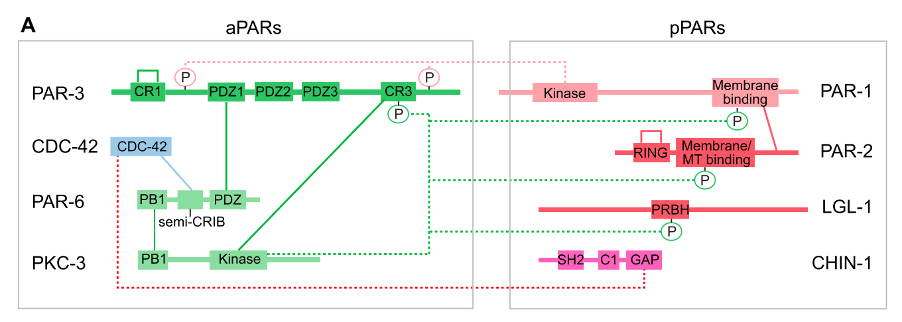
\includegraphics[scale=0.9]{par_proteins_schematic}
\setlength{\abovecaptionskip}{20pt}
\centering
\mycaption{Title}{Caption}
\label{fig:par_proteins_schematic}
\end{figure}


\subsection{Mechanisms of PAR cortical association}

TRANSITION TO SECTION. PAR proteins associate with the cortex in a number of ways. Some PARs display direct and intrinsic cortical localisation activity (PAR-3, PAR-2, CDC-42, CHIN-1, LGL-1). Whilst originally thought to interact with the cytoskeleton, these PARs are now known to localise to the cortex by interacting with the plasma membrane through a combination of electrostatics and specific phospholipid interactions. Other PARs lack intrinsic cortical localisation activity (PAR-6), relying instead on other PARs to act as scaffolds and adaptors, or fall somewhere in between with a mix of direct and scaffold-mediated membrane binding (PAR-1, PKC-3). In this section I will overview some of the key mechanisms.\\


\textit{Association with lipids}\\

% make distinction between lipid interactions and charge based early on

PAR-3, associates with the membrane via its PDZ2 domain \parencite{Li2010a}. <MORE, any research on PDZ2 domains, what is this binding to?>.  The C-terminal portion also plays a role in promoting strong membrane association, although the function of this region isn’t understood (?, I think more is known about it in other species) (Li 2010b). \\

% PKC-3: can bind directly

The membrane localisation of CDC-42 is largely due to a c-terminal geranylgeranyl moiety (REF). MORE HERE. The protein additionally contains a conserved cluster of positively charged residues directly preceding the geranylgeranyl moiety, including a di-arginine motif which promotes specificity for PIP2 containing membranes \parencite{Johnson2012}.\\

Cortical localisation of PAR-2 in vivo depends on a central unstructured region of the protein rich in basic amino acids \parencite{Hao2006}. Full-length PAR-2 displays an ability to bind to an array of positively charged phospholipids in vitro, suggesting an electrostatics-based interaction rather than specific interaction with any one phospholipid \parencite{Motegi2011}. Given this promiscuous nature, its apparent specificity for the plasma membrane in vivo is poorly understood, but may be a consequence of the increased charge associated with this membrane compared to other membranes (REF).\\

PAR-1 contains a C-terminal KA domain, a common membrane association domain, which can bind to membranes and (similarly to PAR-2) interact non-specifically with anionic phospholipids \parencite{Moravcevic2010}. This domain has been shown to be both necessary and sufficient for cortical localisation in vivo \parencite{Motegi2011}.\\

Cortical association of LGL-1 relies on a region towards the C-terminus of the protein, which is rich in positively charged amino acids and can directly bind to negatively charged membranes \parencite{Visco2016}. Independent of overall membrane charge, affinity is strongest for membranes enriched in diphosphoinositides (Visco, NEED TO CHECK), which are most abundant in the inner leaflet of the plasma membrane. Upon membrane binding, the membrane binding domain folds into an alpha-helix, creating a positively charged patch of basic amino acids. Mutations at some, but not all, of these basic amino acids, lowers affinity for diphosphoinositides, suggesting that this folded domain is important for membrane binding specificity. \\


\textit{Interaction with scaffolds}\\

Other PARs lack intrinsic cortical localisation activity, relying instead on other PARs to act as scaffolds and adaptors. PAR-6 and PKC-3 are stable binding partners, interacting via PB1 domains at the N-terminus of each protein (\cite{Hirano2005}), and in normal circumstances are dependent on each other for stable cortical association (refs: Hung, Tabuse). Proper cortical association of this complex relies on interactions with both PAR-3 and CDC-42. PAR-6 interacts with CDC-42 via its semi-CRIB domain, which is a requirement for proper cortical association (\cite{Aceto2006}). It can also interact with the PDZ1 domain of PAR-3 via its own PDZ domain (Li 2010a). However, this interaction doesn't appear to play an essential role in vivo, as mutations to this domain which disrupt the interaction in vitro have no effect on PAR-6 localisation. PKC-3 engages with PAR-3 via its kinase domain. Two sites flanking the phosphosite direct binding to the CR3 domain of PAR-3 \citep{Soriano2016}). Upstream of the phosphosite is an FxR site, a conserved motif found in PKC-3 substrates which provides an anchor point for PKC-3. Downstream is a hook motif which engages pockets within the PKC-3 kinase domain and disrupts an N-lobe required for catalytic activity, keeping PKC-3 in an inactive state.\\

In zygotes, PAR-6/PKC-3 accumulate at the membrane in two distinct pools: a punctate PAR-3 dependent pool, and a diffuse CDC-42 dependent pool \citep{Aceto2006, Beers2006}. The punctate pool represents PAR-6/PKC-3 directly associated with PAR-3 \citep{Dickinson2017}, whereas the diffuse pool represents PAR-6/PKC-3 bound to CDC-42. PAR-3 is usually essential for any PAR-6/PKC-3 localisation, suggesting that the PAR-3 associated state is a prerequisite for assembly into the CDC-42 associated state. Interestingly, however, inhibition of PKC-3 kinase activity allows the complex to bypass this requirement and interact with CDC42 directly in the absence of PAR-3 \citep{Rodriguez2017}. This implies a model where the complex is first recruited into a PAR-3 associated complex <via what interactions?>, PKC-3 is then inactivated by PAR-3 <need details on this: see Soriano>, which permits transfer to a CDC-42 associated state, in which the inhibition of PKC-3 is relieved.\\

Whilst PAR-1 displays some intrinsic lipid binding activity, it’s cortical localisation is largely mediated by interaction with PAR-2. Again, this interaction is via the KA domain of PAR-2, which interacts with an unknown region of PAR-2 \citep{Motegi2011}. This reaction leads to local recruitment of PAR-1 by PAR-2, and cortical localisation in regions of PAR-2 enrichment.\\


\textit{Self-association and clustering}\\

For some PAR proteins, a key determinant for stable association is the ability to self-associate into oligomers, in some cases forming large clusters. PAR-3 contains a CR1 domain at the N-terminus, an oligomerisation domain which assembles into helical filaments in vitro (Feng, Zhang). Oligomerisation of the protein via this domain is essential for stable membrane association in vivo \citep{Dickinson2017} (others: Li 2010, Benton, Feng, Mizuno), although CR1 domain mutants can display transient cortical association (REF). <Comment on this>. Clustering is negatively regulated by PLK-1 phosphorylation, which conveys cell cycle dependence on PAR-3 cortical association. <MORE, REFS, Dickinson>\\

Whilst little is known about the mechanisms of CHIN-1 cortical association, it has also been observed to localise in discrete puncta \citep{Kumfer2010}. These punca only appears during late maintenance phase. It's therefore plausible that, similar to PAR-3, self-association might be under regulatory control.\\

PAR-2 has also been suggested to self-associate and form clusters on the cortex \citep{Arata2016}. <leave main discussion until later>\\


\subsection{Maintenance of polarity by mutual antagonism}

Polarity occurs when the cortical localisation of the PARs is biased, such that the aPARs accumulate on the membrane on one side of the cell, and pPARs on the other. A key component of this is mutual antagonism, whereby proteins within each of the two groups are able to negatively regulate the cortical association of proteins in the other group. There are a number of pathways that contribute to this.\\

\textit{PKC-3 pathway}\\ 

Antagonism from aPARs to pPARs is driven exclusively by PKC-3. <FxR, see Soriano>. Phosphorylation adds negative charge to the proteins, which repels them from the membrane. MORE HERE\\

In the case of PAR-1 and LGL-1, phosphorylation is at a single site within the membrane association domain \citep{Hoege2010, Motegi2011}. Phosphorylation of these sites is necessary and sufficient to exclude these proteins from the membrane. PAR-2 is more complex, with seven predicted phosphorylation sites \citep{Hao2006}, although these have yet to be verified biochemically. Some of these are within the membrane association domain, and likely regulate membrane association in an analogous way to PAR-1 and LGL-1. Phosphorylation by PKC-3 has been shown to disrupt binding of PAR-2 to phospholipids in vitro, which is thought to represent reduced electrostatic attraction via the addition of negatively charged phosphate groups to the protein \citep{Motegi2011}. Some of the predicted phosphorylation sites are outside the membrane association region and may play regulatory or gatekeeping roles. Mutation of all seven sites prevents phosphorylation in vivo, leading to uniform PAR-2 \citep{Hao2006}). Whilst individual mutant analysis hasn't been performed on all of these sites independently, \textcite{Motegi2011} show that mutation of just one of these sites (S241A) significantly reduces phosphorylation in vitro and achieves the same phenotype as the 7S/E mutant in vivo, indicating that this site may play a key role as a gatekeeper. Phosphomimetic mutation of all seven sites weakens, but doesn't completely eliminate membrane association, indicating that there may additional sites on the protein, or that these mutations fail to completely mimic phosphorylation (what’s the charge of E compared to a phosphate?). \\

CHIN-1 doesn’t have an FxR site (check), but is also excluded from the anterior by PKC-3 \citep{Sailer2015}. This is thought to involve direct inhibition of CHIN-1 clustering at the cortex by PKC-3, however the mechanistic basis of this is poorly understood.\\

\textit{PAR-1 pathway} \\

PAR-1 can phosphorylate PAR-3, which it does primarily at a single serine (S950) towards the C-terminus of the protein \citep{Motegi2011}. <REGULATES CLUSTERING> In a wild-type background, depletion of PAR-1, or mutation of the phosphosite on PAR-3, causes PAR-3 to associate with the posterior cortex, although this association is still relatively weak \citep{Sailer2015}. It is unclear why some degree of asymmetry is maintained in these conditions, although this may be a remnant of earlier transport by cortical flows and relatively stable cortical association which prevents lateral diffusion and cortical-cytoplasmic exchange that would redistribute the protein. If cortical flows are inhibited, PAR-1 loss prevents aPARs from polarising at all \citep{Motegi2011}.\\

\textit{LGL-1 pathway}\\

LGL-1 has been proposed to antagonise aPARs by forming a complex with PAR-6/PKC-3, the whole of which dissociates from the cortex after LGL-1 is phosphorylated by PKC-3 \citep{Hoege2010}. LGL-1 loss has no observable effects in zygotes in otherwise wild type systems, indicating that this is usually of minor importance, but can enhance phenotypes in PAR-2 mutants \citep{Beatty2010}. Furthermore, LGL-1 overexpression is able to compensate for absence of PAR-2 \citep{Hoege2010}, indicating that this pathway can be sufficient to take over the roles of the PAR-2/PAR-1 pathway.\\

\textit{CHIN-1 pathway}\\

CHIN-1, a GAP for CDC-42 appears on the posterior cortex late in the cell cycle and restricts CDC-42 activity to the anterior \citep{Kumfer2010} \citep{Beatty2013, Sailer2015}. CHIN-1 loss results in uniform CDC-42 activity, but this doesn't lead to uniform PAR-6/PKC-3 localisation (Sailer, others), indicating that active CDC-42 isn’t sufficient to recruit PAR-6/PKC-3. When combined with a PAR-1 mutant, however, which leads to a small amount of PAR-3 binding in the posterior, PAR-6/PKC-3 is now recruited to a high level in the posterior. This implies that PAR-3 gates association with CDC-42. PAR-3 asymmetry is required to restrict this gating to the anterior, and CDC-42 asymmetry is required to restrict the binding partner of PAR-6/PKC-3 to the anterior, although either one of these behaviours is sufficient to enforce a degree of asymmetry.\\


\subsection{Establishment of polarity}

As previously mentioned, PAR polarity doesn't occur spontaneously, requiring a trigger so that polarity happens at the correct time and with the correct orientation. Prior to the establishment of asymmetry, aPARs are uniformly enriched on the cortex, and exclude pPARs through antagonistic interactions. Polarity is then triggered by signals from the MTOC which forms near the site of sperm entry, via two redundant pathways:\\

\textit{Anterior-directed cortical flows}\\

A first mechanism involves a local inhibition of RhoA activity in the posterior of the cell, which downregulates actomyosin contractility. This sets up a spatial gradient of contractility, which leads to anterior-directed cortical flows. The aPARs PAR-3, PAR-6 and PKC-3 are advected by these flows, which causes them to segregate to the anterior. <more here on local RhoA inhibition, par-3 clustering>\\

The resulting depletion of PKC-3 concentration in the posterior relieves antagonism of pPARs, allowing them to bind in the posterior and form a nascent domain. This domain is then amplified via a series of antagonistic feedback reactions, which are described in another section. This mechanism of advective triggering followed by self-organisation is sufficient to capture the core features and dynamics of polarity in computer models of the PAR network \citep{Goehring2011a}.\\

Further work has shown that the PAR proteins themselves are able to feed back onto the actomyosin cortex, amplifying contractility asymmetries as polarity progresses \citep{Gross2018} <More here>.\\

Whilst primarily important during establishment phase, continued regulation of cortical flow by the PAR proteins also plays a role in preventing the breakdown of polarity during maintenance phase. In par-2 mutants, whilst anterior-directed cortical flow proceeds as normal during polarity establishment (Gross CHECK), these are followed by aberrant posterior-directed cortical flows at maintenance phase, leading to significant spread of aPARs back towards the posterior (ref). The precise mechanistic reasons for this misregulation in PAR-2 mutants is unclear, but it suggests that signalling from PAR-2 plays some role in preventing rearwards cortical flows at maintenance phase.  PAR-2 loss leads to higher cortical myosin accumulation independently of PAR-6/PKC-3 presence \citep{Munro2004, Beatty2013}, suggesting that this isn't an indirect effect via PKC-3 signalling. Backwards flows can be prevented by mutation of MRCK-1, <details on this protein>.\\

LGL-1 can also regulate maintenance phase flows in a similar way. Dual loss of PAR-2 and LGL-1 leads to stronger rearwards flow \citep{Beatty2010}, and overexpression of LGL-1 is able to rescue rearwards flow in PAR-2 mutants \citep{Hoege2010}. However, unlike PAR-2, LGL-1 has no effect on myosin accumulation in the absence of PAR-6, suggesting that this LGL-1 dependent effect may be indirect via aPARs and the known roles of PKC-3 in cytoskeleton control (i.e. LGL-1 loss weakens antagonism, leading to aPAR invasion, which redistributes flows).\\

\textit{The microtubule pathway}\\

In the absence of cortical flows, symmetry breaking still occurs, albeit later, indicating the existence of multiple symmetry breaking mechanisms. A second triggering mechanism involves an interaction between PAR-2 and microtubules emanating from the sperm-donated centrosome. In no-flow regimes, PAR-2 symmetry breaking occurs late, and correlates spatially and temporally with the site of MTOC-cortex contact \citep{Motegi2011}. Treatments that disrupt microtubules prevent symmetry breaking in these conditions.\\

Mechanistically, this is carried out by a direct interaction between PAR-2 and microtubules, which is thought to shield the phosphorylation sites on PAR-2, and has been shown to reduce phosphorylation by PKC-3 in vitro \citep{Motegi2011}. This creates a zone of local protection in the posterior of the cell, allowing PAR-2, and thus PAR-1 to load, kicking of self-organisation. Mutations at the microtubule binding interface on PAR-2 have a similar phenotype to nocodazole treatments.\\

\textit{Additional pathways}\\

Additional mechanisms may underlie triggering in some circumstances. <Evidence of still breaking symmetry when other cues are lost>. Microfabrication studies show that PAR-2 has a preference for curved membranes. This may lead to preferential binding of PAR-2 at the poles of cells, which has been suggested to act as a symmetry breaking cue in cases where normal symmetry breaking is misregulated \citep{Klinkert2019}. The mechanistic basis for this proposed curvature sensitivity is unclear.\\


\subsection{Downstream of the PAR proteins}

The primary role of the PAR proteins is to regulate an asymmetric cell division, whereby the P0 divides to give two cells differing in size and fate. This is carried out via two pathways:\\

\textit{Placement of the division plane}\\

Signalling from the PARs regulates the position of the mitotic spindle, which leads to a cell size asymmetry following cytokinesis. This is carried out predominantly by PKC-3, which phosphorylates <> LIN-5. This results in decreased microtubule pulling forces in the anterior, where PKC-3 is highest, leading to a shift in the position of the mitotic spindle towards the posterior. PAR-2 also has a direct effect on spindle pulling forces through an unknown mechanism, independently of aPARs, which may contribute to placement of the division plane (Rodrigues).\\


\textit{Segregation of fate determinants}\\

As well as differing in size, the two daughter cells differ in a number of cytoplasmic components which define cell fate during development, which is also set up by signalling from the PARs. Immediately downstream of the PARs is MEX-5, which is organised into a cytoplasmic gradient in response to asymmetry of PAR-1. PAR-1 phosphorylates MEX-5 \citep{Griffin2011}, which increases its mobility. Working against the action of a uniform phosphatase, PP2A, this leads to an asymmetry in MEX mobility, which leads to accumulation at the anterior where mobility is lowest. <Computer models, Griffin>. \\

This MEX gradient then sets up a P granule asymmetry by regulating growth and dissolution of phase-separated P-granule droplets \citep{Brangwynne2009}. These granules dominate in the posterior, so are inherited by the P1 cell after cell division. The granules contain fate determinants which are responsible for specifying germ-line fate in the P lineage.\\


\subsection{Resistance and substrate competition}

\subsection{Discussion}

\clearpage
\section{PAR-2: roles and mechanisms of action}
\subsection{Main functional roles of PAR-2}

To summarise some of the information in the previous sections, the main roles for PAR-2 are as follows:\\

\textbf{Recruitment of PAR-1}. This plays a key role in preventing PAR-3 from associating to the cortex in the posterior, although other mechanisms contribute to keeping PAR-3 in the anterior, which isn;t understood (refs). This acts redundantly with the CHIN-1 pathway to keep the kinase PKC-3 out of the posterior (Sailer, others), and LGL-1 may also contribute to this (Hoege, Beatty, others). \\

Interestingly, despite the role for PAR-1 in segregation of fate determinants, PAR-2 this appears dispensable for proper segregation of fate determinants in in the zygote. Whilst absent from the cortex in these zygotes lacking PAR-2, PAR-1 is still able to maintain a cytoplasmic concentration and activity gradient (mechanism?), meaning that MEX-5 and P-granule asymmetries are largely intact. Notably, however, localisation of fate determinants is impaired at later stages in the embryo in these conditions. Thus, a primary function of the PAR-1/PAR-2 interaction may be to ensure that PAR-1 is segregated and enriched through the germ line, so that downstream signalling can continue in, and be restricted to, the developing P-lineage. \\

\textbf{Protection of PKC-3 substrates}. PAR-2 has been demonstrated to protect both PAR-1 and itself from the antagonistic action of PKC-3 (Motegi, others). In the case of PAR-1, this involves direct shielding of the phosphorylation site on PAR-1 as well as competitive inhibition \citep{Ramanujam2018}. It’s plausible that a similar competitive inhibition mechanism may operate to protect other PKC-3 substrates, namely LGL-1 and CHIN-1, although this hasn't been formally tested. In the case of cortical PAR-2 being able to protect other PAR-2 molecules, the mechanism isn't clear. Competitive inhibition may contribute, and the RING domain of the protein has also been implicated in self-recognition, as described below. \\

\textbf{Restriction of cortical flows at maintenance phase}. PAR-2 appears to play a direct role in preventing rearwards flows at maintenance phase which would otherwise redistribute aPARs to the posterior. The mechanistic basis of this is not understood.\\

\textbf{Signalling to the mitotic spindle}. May contribute to placement of the division boundary, although the mechanism is unclear.\\


\subsection{Evidence and proposed roles for oligomerisation}

As previously mentioned, PAR-2 has been suggested to oligomerise, which may stabilise membrane association. This claim is based primarily on a study by \textcite{Arata2016}. By TIRF imaging, the authors were able to resolve distinct PAR-2 particles of varying size at the cortex, which showed a slight asymmetry towards larger oligomers at the posterior. Based on fluorescence intensity, the largest particles were estimated to be at least tetrameric. Membrane lifetime was found to vary across the cell according to oligomer size and local PKC-3 concentration, indicating that oligomerisation can increase, and phosphorylation decrease, stability of membrane binding. They also found an asymmetry in the membrane association rate, highest in the posterior of polarised cells, which they suggest could be due to direct recruitment of cytoplasmic PAR-2 into cortical oligomers.\\

This ability to self-associate is supported by in vitro pull-down studies, which show that tagged PAR-2 is able to pull down untagged PAR-2 \citep{Motegi2011, Arata2016}. These reports show that the amount pulled down is very small, indicating a weak, non-constitutive interaction. However, quantitative measurements of dimer affinity and oligomer size using biophysical methods have not been performed.\\

Taken together, \textcite{Arata2016} propose that an initial PKC-3 asymmetry leads to a PAR-2 oligomer size asymmetry, either as a direct effect of phosphorylation disrupting oligomerisation, or as a result of concentration-dependent oligomer growth/dissociation. Oligomer size asymmetry would in turn stabilise concentration asymmetries, through on and off rate effects, leading to a degree of positive feedback and polarity stabilisation.\\

Whilst the core-concepts of their model (namely concentration/phosphorylation dependent oligomerisation, oligomer-size dependent membrane stability, and self-recruitment) are attractive and intuitive, they have yet to be formalised by mechanistic computer models in the context of PAR-2 polarity. Furthermore, the mechanistic basis of the putative PAR-2 oligomerisation reaction remains elusive.\\


\subsection{Roles for the RING domain}

Studies of mutant PAR-2 alleles have demonstrated an important role for the N-terminal RING domain in establishing strong PAR-2 domains. Mutations to the putative zinc coordinating residues in the RING domain, designed to misfold the domain and render it non-functional, weaken the strength of PAR-2 cortical localisation \citep{Hao2006}. This is accompanied by faster cortical dynamics as revealed by FRAP, indicative of a shorter membrane lifetime \citep{Motegi2011}. Whilst these mutants can form posterior domains at establishment phase (albeit weakly concentrated), they are rapidly cleared by invading aPARs at maintenance phase \citep{Hao2006}.\\

The mechanistic basis of this mutant phenotype is poorly understood, and perhaps surprising given that the RING domain is distinct from the cortical localisation domain of the protein and shows no cortical binding activity in isolation \citep{Hao2006}. RING mutants show reduced membrane affinity even in the absence of aPARs, indicating that the phenotype is, at least partially, intrinsic to PAR-2, rather than through increased sensitivity to aPARs. It is also unlikely that reduced membrane association is entirely a secondary consequence of the unfolded domain in cysteine mutants, as truncation mutants lacking the domain show a qualitatively similar phenotype, although a quantitative comparison hasn’t been performed.\\

Studies on RING mutants also shed potential light on the mechanisms of PAR-2 protection. \textcite{Hao2006} showed that RING mutants are unable to be protected by endogenous PAR-2 in PAR-1 mutant conditions in which aPARs become uniform, suggesting that the RING may be required to react to endogenous PAR-2. Whilst unclear at the time of the study, more recent work showing that PAR-2 can oligomerise, as described above, along with a characteristic role of RING domains in oligomerisation, as described below, may shed potential light on this. However, this hypothesis is yet to be formally tested. Intriguingly, however, Motegi showed that in near identical experimental conditions RING mutant PAR-2 can (seemingly) be protected by endogenous PAR-2. The reason behind this discrepancy is unclear.\\


\subsection{Discussion}

%%%%%%%%%%%%%%%%%%%%%%%%%%%%%%%%%%%%%%%%%%%%%%%%%%%%%%%%%%
\clearpage
\chapter{A pipeline for quantification of membrane and cytoplasmic protein concentrations}

\textbf{Detailed contributions:}\\

\textbf{Manuscript details:}

\clearpage
\section{Introduction}

Intro to section, build on narrative from previous section

\clearpage
\section{Autofluorescence correction}

\textit{Note: this section has been adapted from \textcite{Rodrigues2022}, and describes work performed with Nelio Rodrigues.}

\subsection{Autofluorescence in \textit{C. elegans}}

One major barrier in quantitative experiments using \textit{C. elegans} is autofluorescence (AF), which is particularly prominent in channels excited with blue wavelengths which are commonly used to image green fluorophores. When using endogenously tagged proteins, which are often expressed at low levels, this contribution can often be a significant fraction of the total signal, and can therefore significantly obscure the true signal that one is interested in. This might pose particular problems for quantitative experiments, where the absolute signal levels may be important.\\

We can observe the significance of the problem in \textit{C. elegans} by imaging untagged control embryos. As shown in \cref{fig:saibr_n2_vs_lgl} (left panels), a significant amount of signal is collected in the regular GFP channel (488nm excitation, 535/50nm emission), which varies both spatially within the image, and between different images. By comparison, total signal in embryos endogenously tagged with LGL-1::GFP ( \cref{fig:saibr_n2_vs_lgl}, right panels) is also highly variable, and only marginally higher than N2s, suggesting that a significant fraction of the total signal observed in these cells is autofluorescence, and that much of the intra-embryo signal variation is likely due to variable autofluorescence. Despite being enriched at the posterior membrane, which is easily visible in cells with overexpressed LGL-1 (e.g. \cite{Hoege2010}), this is difficult to visualise here as a result of autofluorescence. Therefore, if we want to accurately visualise, and indeed quantify, protein levels and distributions, we need a method that can locally correct AF on a pixel-by-pixel basis.\\

\begin{SCfigure}
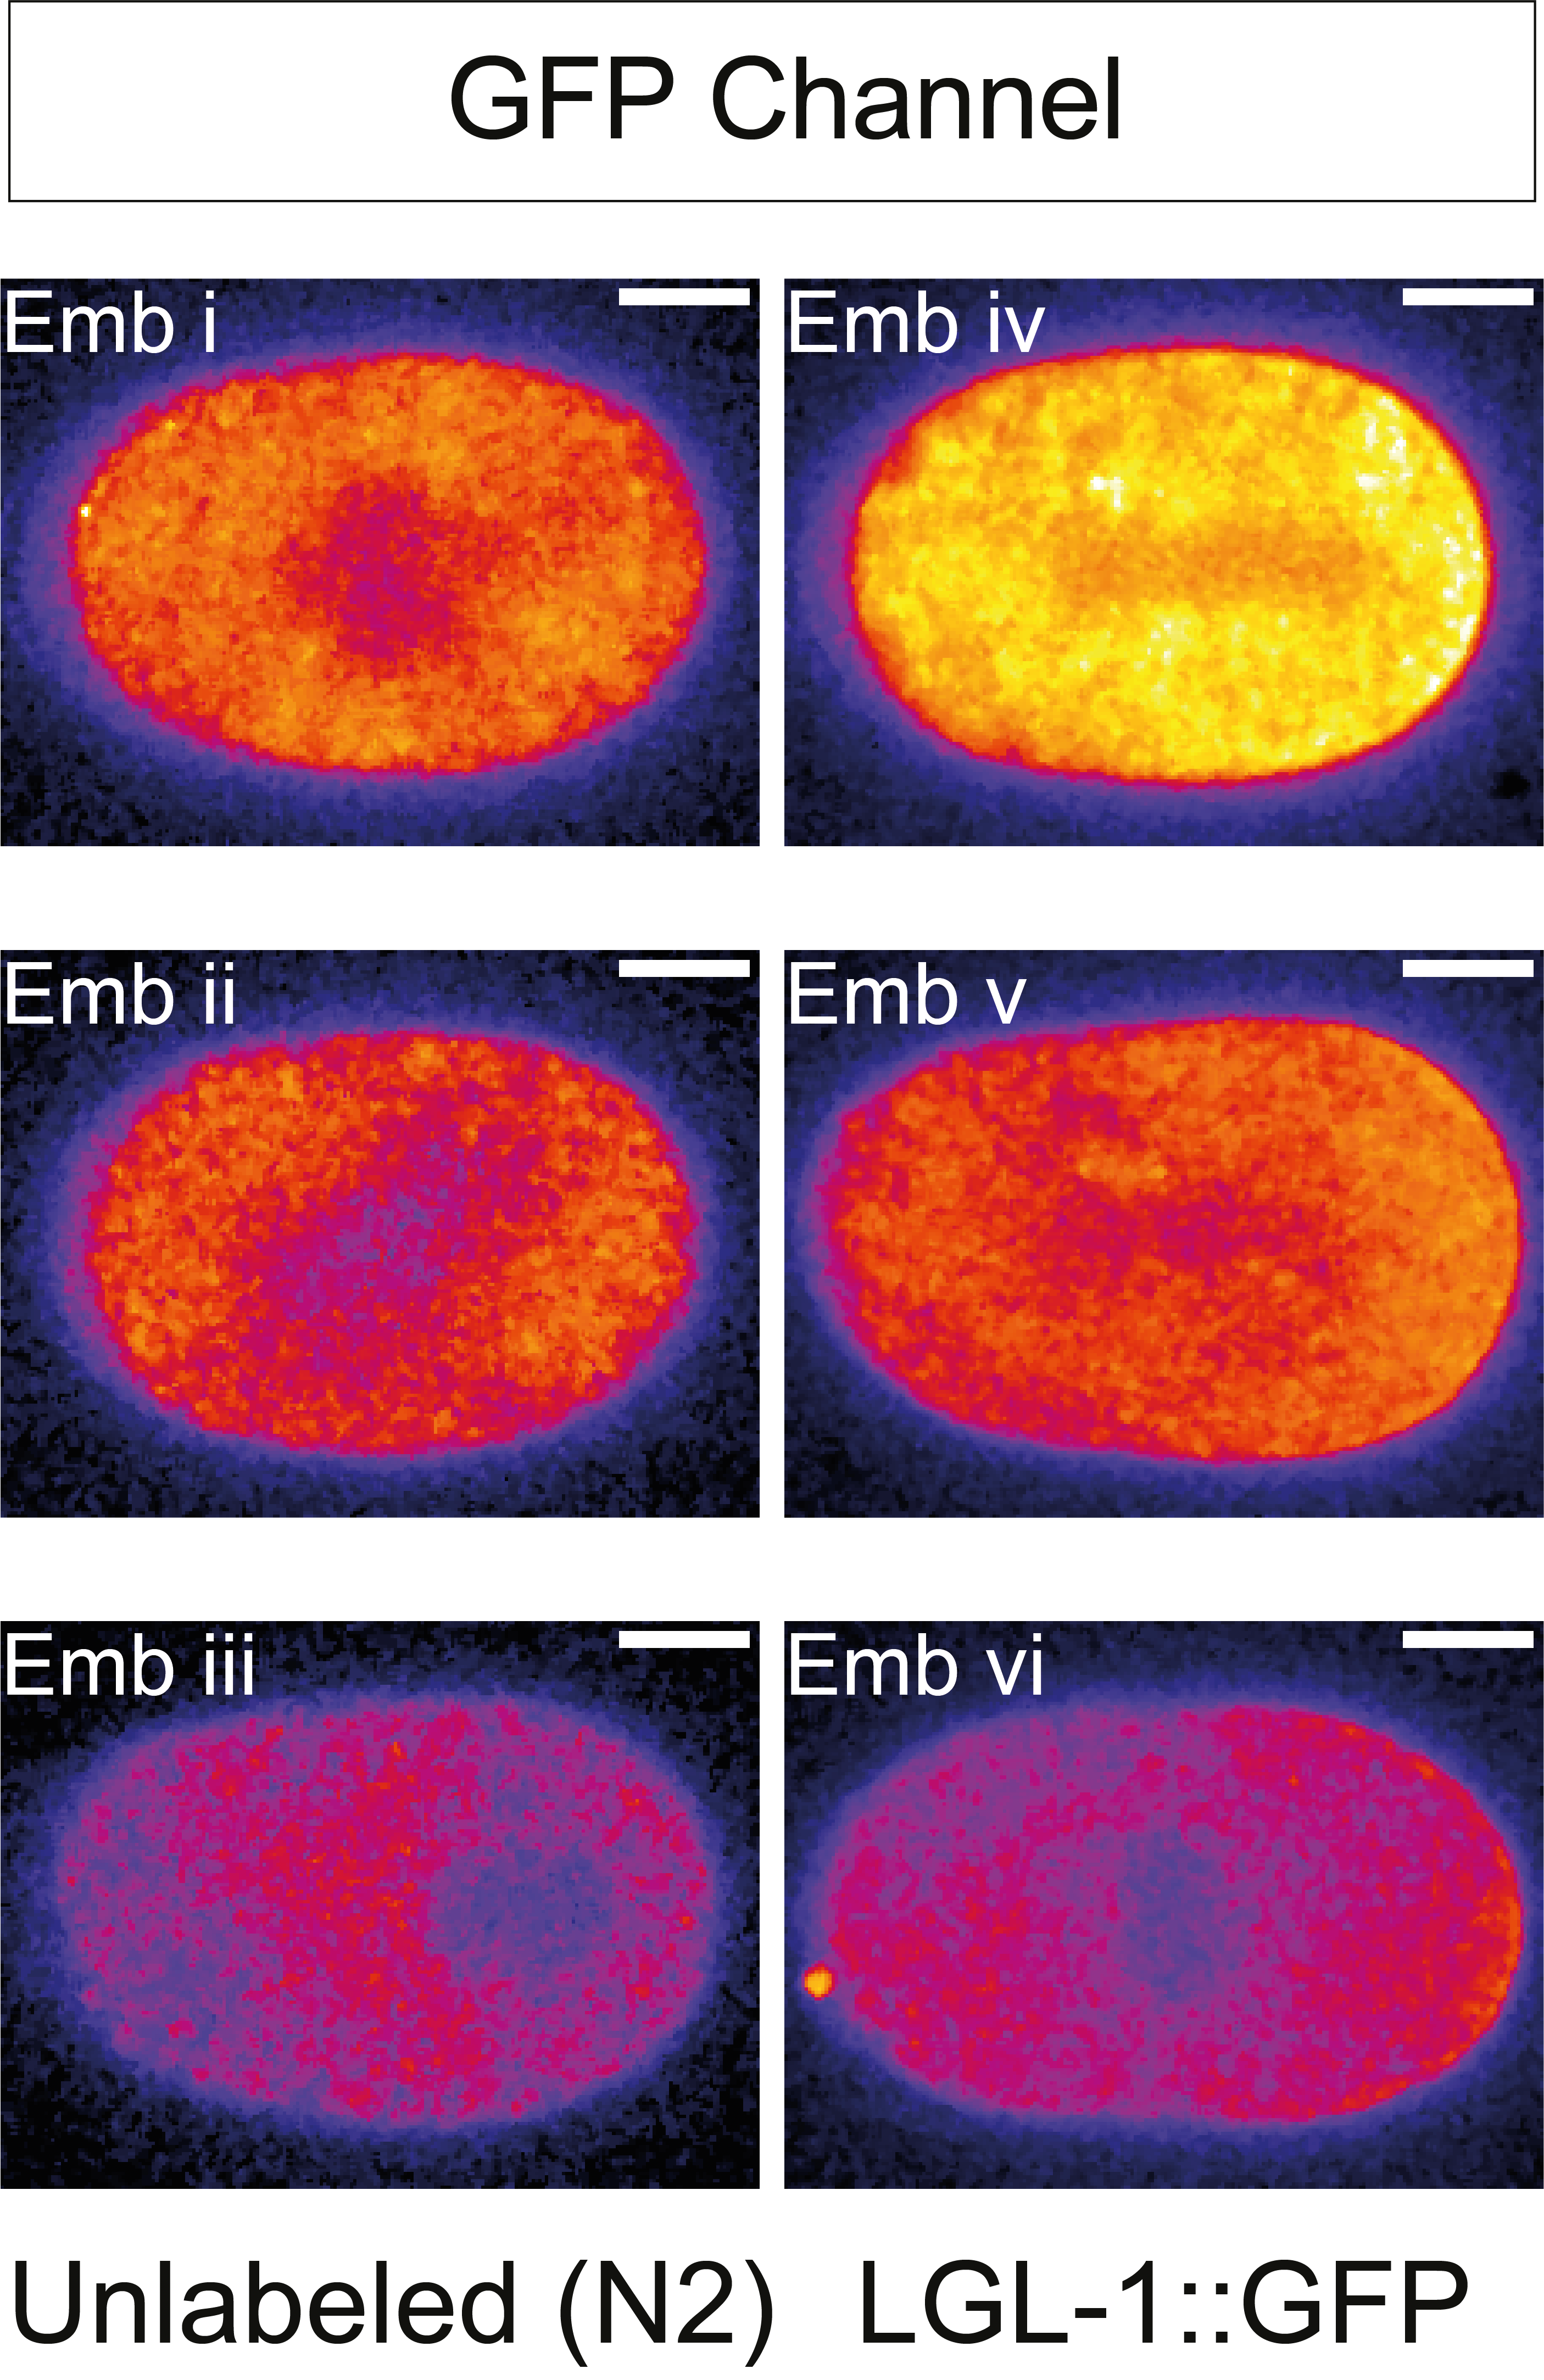
\includegraphics[scale=0.9]{saibr_n2_vs_lgl}
\mycaption{Autofluorescence is abundant and variable in images of \textit{C. elegans} zygotes}{GFP channel (488nm excitation, 535/50nm emission) images of unlabelled N2 and LGL-1::GFP embryos taken under identical imaging conditions. Pixel scaling is the same for each image. Fig. 1B from \textcite{Rodrigues2022}.}
\label{fig:saibr_n2_vs_lgl}
\end{SCfigure}

One approach that has been used to tackle autofluorescence in some systems is spectral imaging \citep{Billinton2001}. Typically used to separate overlapping fluorophore signals based on spectral characteristics, this approach can also be used to separate out autofluorescence by treating it much like a fluorophore with its own spectral characteristics. Whilst often effective, these techniques require specialised instruments and analysis tools and cannot be performed on standard confocal microscopes.\\

A simpler, related, approach has been proposed for some systems (e.g. \cite{Roederer1986}) which exploits the fact that autofluorescence can often be described as a single fluorescent component, with an emission spectrum much broader than GFP. If one can find an emission wavelength (usually red shifted) that is specific for autofluorescence, this can be used to infer the amount of autofluorescence in the sample, which can then be subtracted away from the regular fluorophore channel to give a clean readout of fluorophore signal. In comparison to full spectral imaging, this method can be carried out with standard light sources and emission filters, and therefore can be easily implemented into existing workflows.\\

Inspired by this approach, we aimed to implement, and assess the applicability of such a method for autofluorescence removal in images of \textit{C. elegans} embryos. In doing so, we have put together a robust and easily-implementable workflow which we’ve termed SAIBR: Spectral Autofluorescence Image correction by Regression.\\


\subsection{SAIBR: a simplified method for autofluorescence correction based on dual emission imaging}


At minimum, autofluorescence correction relies on the ability to find a reporter channel that is free of GFP signal, but rich in autofluorescence, such that this channel can be used as an independent readout of autofluorescence in the sample. Full spectral analysis performed by Nelio Rodrigues (not shown here), shows that a channel with a red shifted emission filter, such as those commonly used to image red fluorescent proteins, meets such a requirement.\\

Furthermore, by imaging untagged embryos with both the standard GFP channel and this red-shifted autofluorescence-reporter channel (488nm excitation, 630/75nm emission), which I will refer to as the AF channel, we find a strong linear correlation between pixel data from the two channels (\cref{fig:saibr_n2_correlation}). Whilst raw pixel values do not correlate well, as these are dominated by noise, we can get a strong correlation by first applying a Gaussian filter to suppress this noise (\cref{fig:saibr_n2_correlation}A). We found that this relationship is consistent between embryos (\cref{fig:saibr_n2_correlation}B, C). Furthermore, we found a near identical relationship when plotting the mean intensity values of individual embryos, suggesting that the same relationship can account for both intra- and inter-embryo AF variation. \\

\begin{figure}
\includegraphics[scale=0.95]{saibr_n2_correlation}
\centering
\mycaption{Autofluorescence is spatially correlated across emission channels}{
\textbf{(A)} Correlation of pixel values between the GFP channel and AF channel for an unlabelled N2 embryo, subject to Gaussian blur of indicated radius. Pixel values were taken from an ROI encompassing the entire embryo and a portion of the background. All pixels within this region were used for the regression, but for clarity only a random 10\% sample of pixels are shown.
\textbf{(B)} Comparison of inter-channel pixel correlation (Gaussian radius = 1) for three unlabelled N2 embryos, colour coded by embryo. Histograms of intensity values for GFP and AF channels shown for reference.
\textbf{(C)} Comparison of per-pixel correlation with data obtained from whole embryo means. (i) Lines indicate per-pixel regression for individual embryos as in (B). (ii) Overlay showing mean whole embryo fluorescence values (circles).
Fig. S2 and 1E-F from \textcite{Rodrigues2022}.
}
\label{fig:saibr_n2_correlation}
\end{figure}

Together, this implies that taking an AF channel image should be sufficient to accurately predict the level of autofluorescence in the GFP channel, and thus subtract it out. To quantify the necessary inter-channel conversion factors, I performed linear regression, using an ordinary least squares method, on Gaussian-filtered pixel values pooled from multiple untagged embryos. Then, to perform correction on images containing fluorophore, we just need to capture an AF channel image, alongside the GFP channel image, rescale the AF image according to the predefined conversion factors, and then subtract this inferred autofluorescence away from the GFP channel image pixel-by-pixel.\\


\subsection{Assessing SAIBR performance on images of PAR proteins}

To assess the effectiveness of SAIBR, and it’s utility in the analysis of PAR proteins, I applied it to a range of images of unlabelled and GFP-labelled embryos. As expected, applying SAIBR to images of unlabelled cells reduced fluorescence from across the cells to zero, with no visible structures remaining (\cref{fig:saibr_spatial_correction}A). This is a good validation of the method, and suggests that it can properly account for all of the autofluorescence in the cell. \\

In the case of LGL-1::GFP expressing embryos, where autofluorescence signal is dominant (\cref{fig:saibr_n2_vs_lgl}), SAIBR removes autofluorescence signal within the cell, and improves contrast at the posterior cortex, allowing us to better resolve plasma membrane enrichment \cref{fig:saibr_spatial_correction}B. Improvements are just as striking for PAR-3::GFP. In addition to improvements at the cortex, we see that SAIBR can suppress the local fluorescence minimum at the cell centre caused by lower AF at the pronuclei. For PAR-6::GFP the improvements are qualitatively less striking, as the ratio of fluorophore signal to autofluorescence is higher, but nonetheless AF removal has a quantitative impact.\\

\begin{figure}
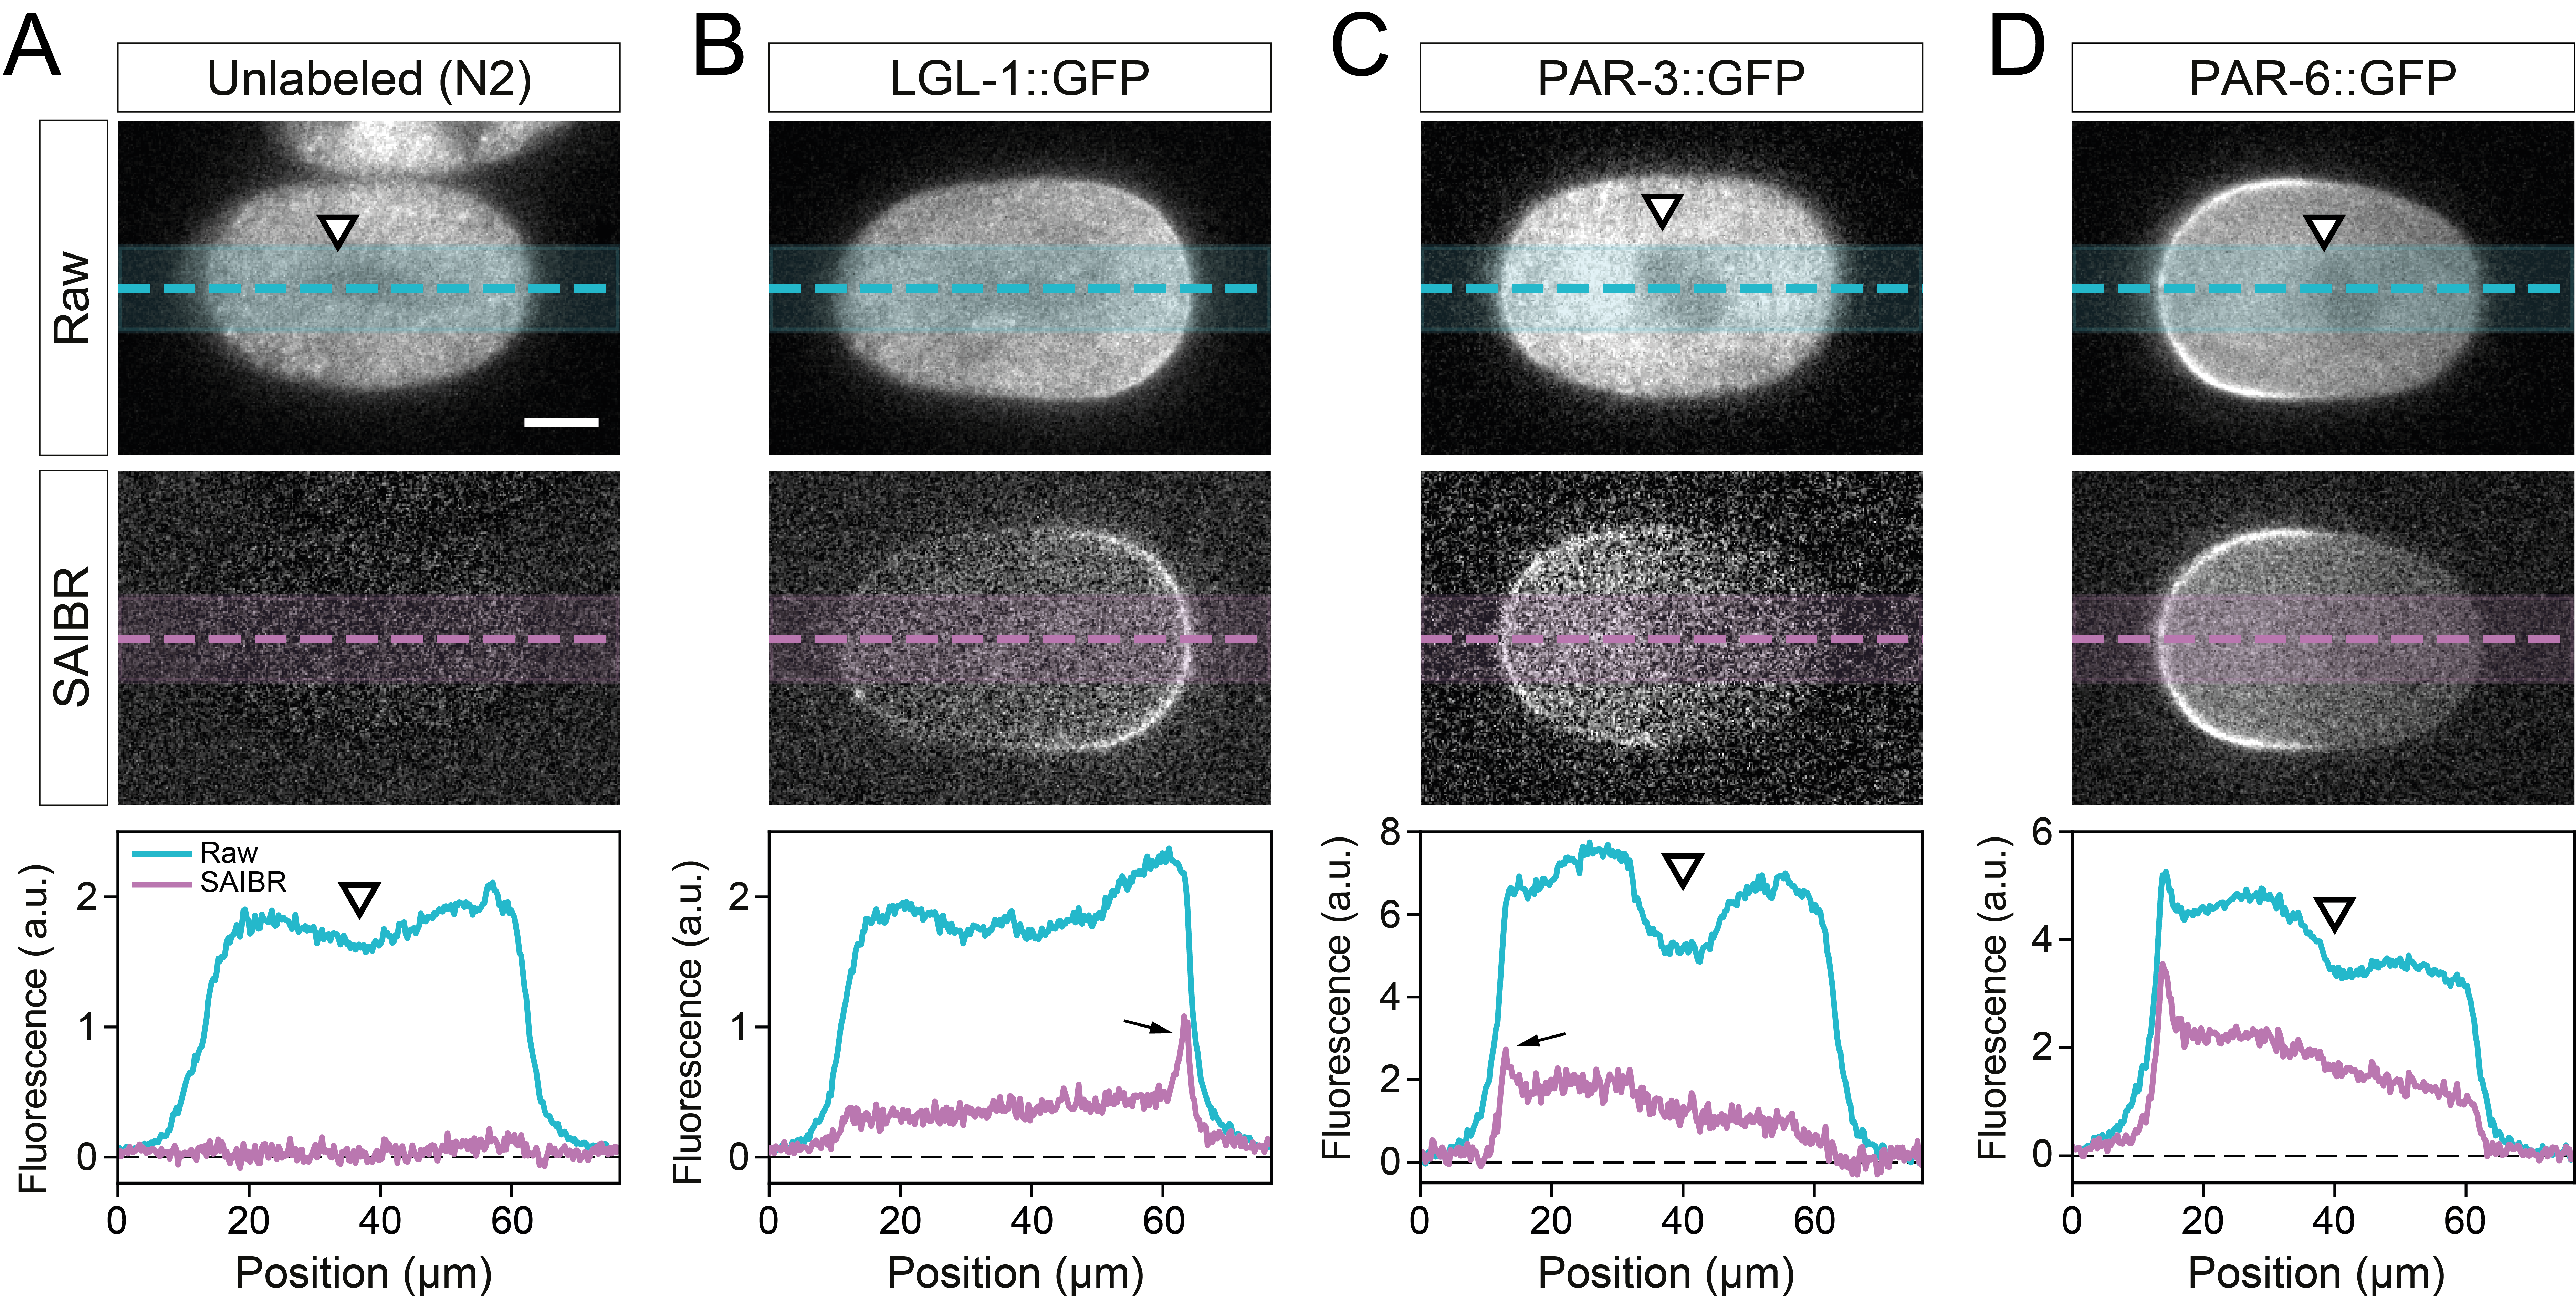
\includegraphics[scale=0.9]{saibr_spatial_correction}
\centering
\mycaption{Applying SAIBR to images of GFP-tagged PAR proteins}{
\textbf{(A) - (D)} Raw (top) and SAIBR-corrected (middle) midplane images of zygotes expressing the indicated GFP fusions. Bottom panels show associated linescans across the images. SAIBR reveals prominent membrane localisation for LGL-1 and PAR-3 (arrows) which is not obvious in uncorrected images. We also see a prominent signal dip in the pronuclear region of uncorrected images due to local exclusion of autofluorescence (arrowheads), which disappears in SAIBR corrected images.
Fig. 2A-D from \textcite{Rodrigues2022}.}
\label{fig:saibr_spatial_correction}
\end{figure}

As shown in \cref{fig:saibr_membrane_profiles}, SAIBR has a strong impact on the shape of intensity profiles taken across the cortex within each polarity domain, in all cases showing a clearer peak and suppression of signal at the internal portion of the curves. This has particular importance for quantitative studies as, as described in section \ref{section:memquant}, the shape of cross-cortex profiles are often used to quantitatively analyse membrane concentrations and/or membrane affinities. For example, a cross-cortex profile with a central peak that is much higher than the internal cytoplasmic plateau clearly implies that the protein is binding to the membrane with a high affinity. We can see from the SAIBR corrected profiles that, of the three proteins shown here, LGL-1 has the strongest membrane affinity (highest enrichment at the membrane compared to its cytoplasmic level), followed by PAR-6, followed by PAR-3. If we look at the profiles pre-correction, however, this isn't so clearly apparent. One might have had some success by simply subtracting an equivalent average profile taken from untagged N2s, but such a method would fail to account for the fact that much of variation between embryos is down to autofluorescence, and would therefore be unsuitable for studies where inter-embryo variation is important. In the case of LGL-1 this would also clearly result in negative values at the cytoplasmic portion of the curve for some embryos.\\

\begin{figure}
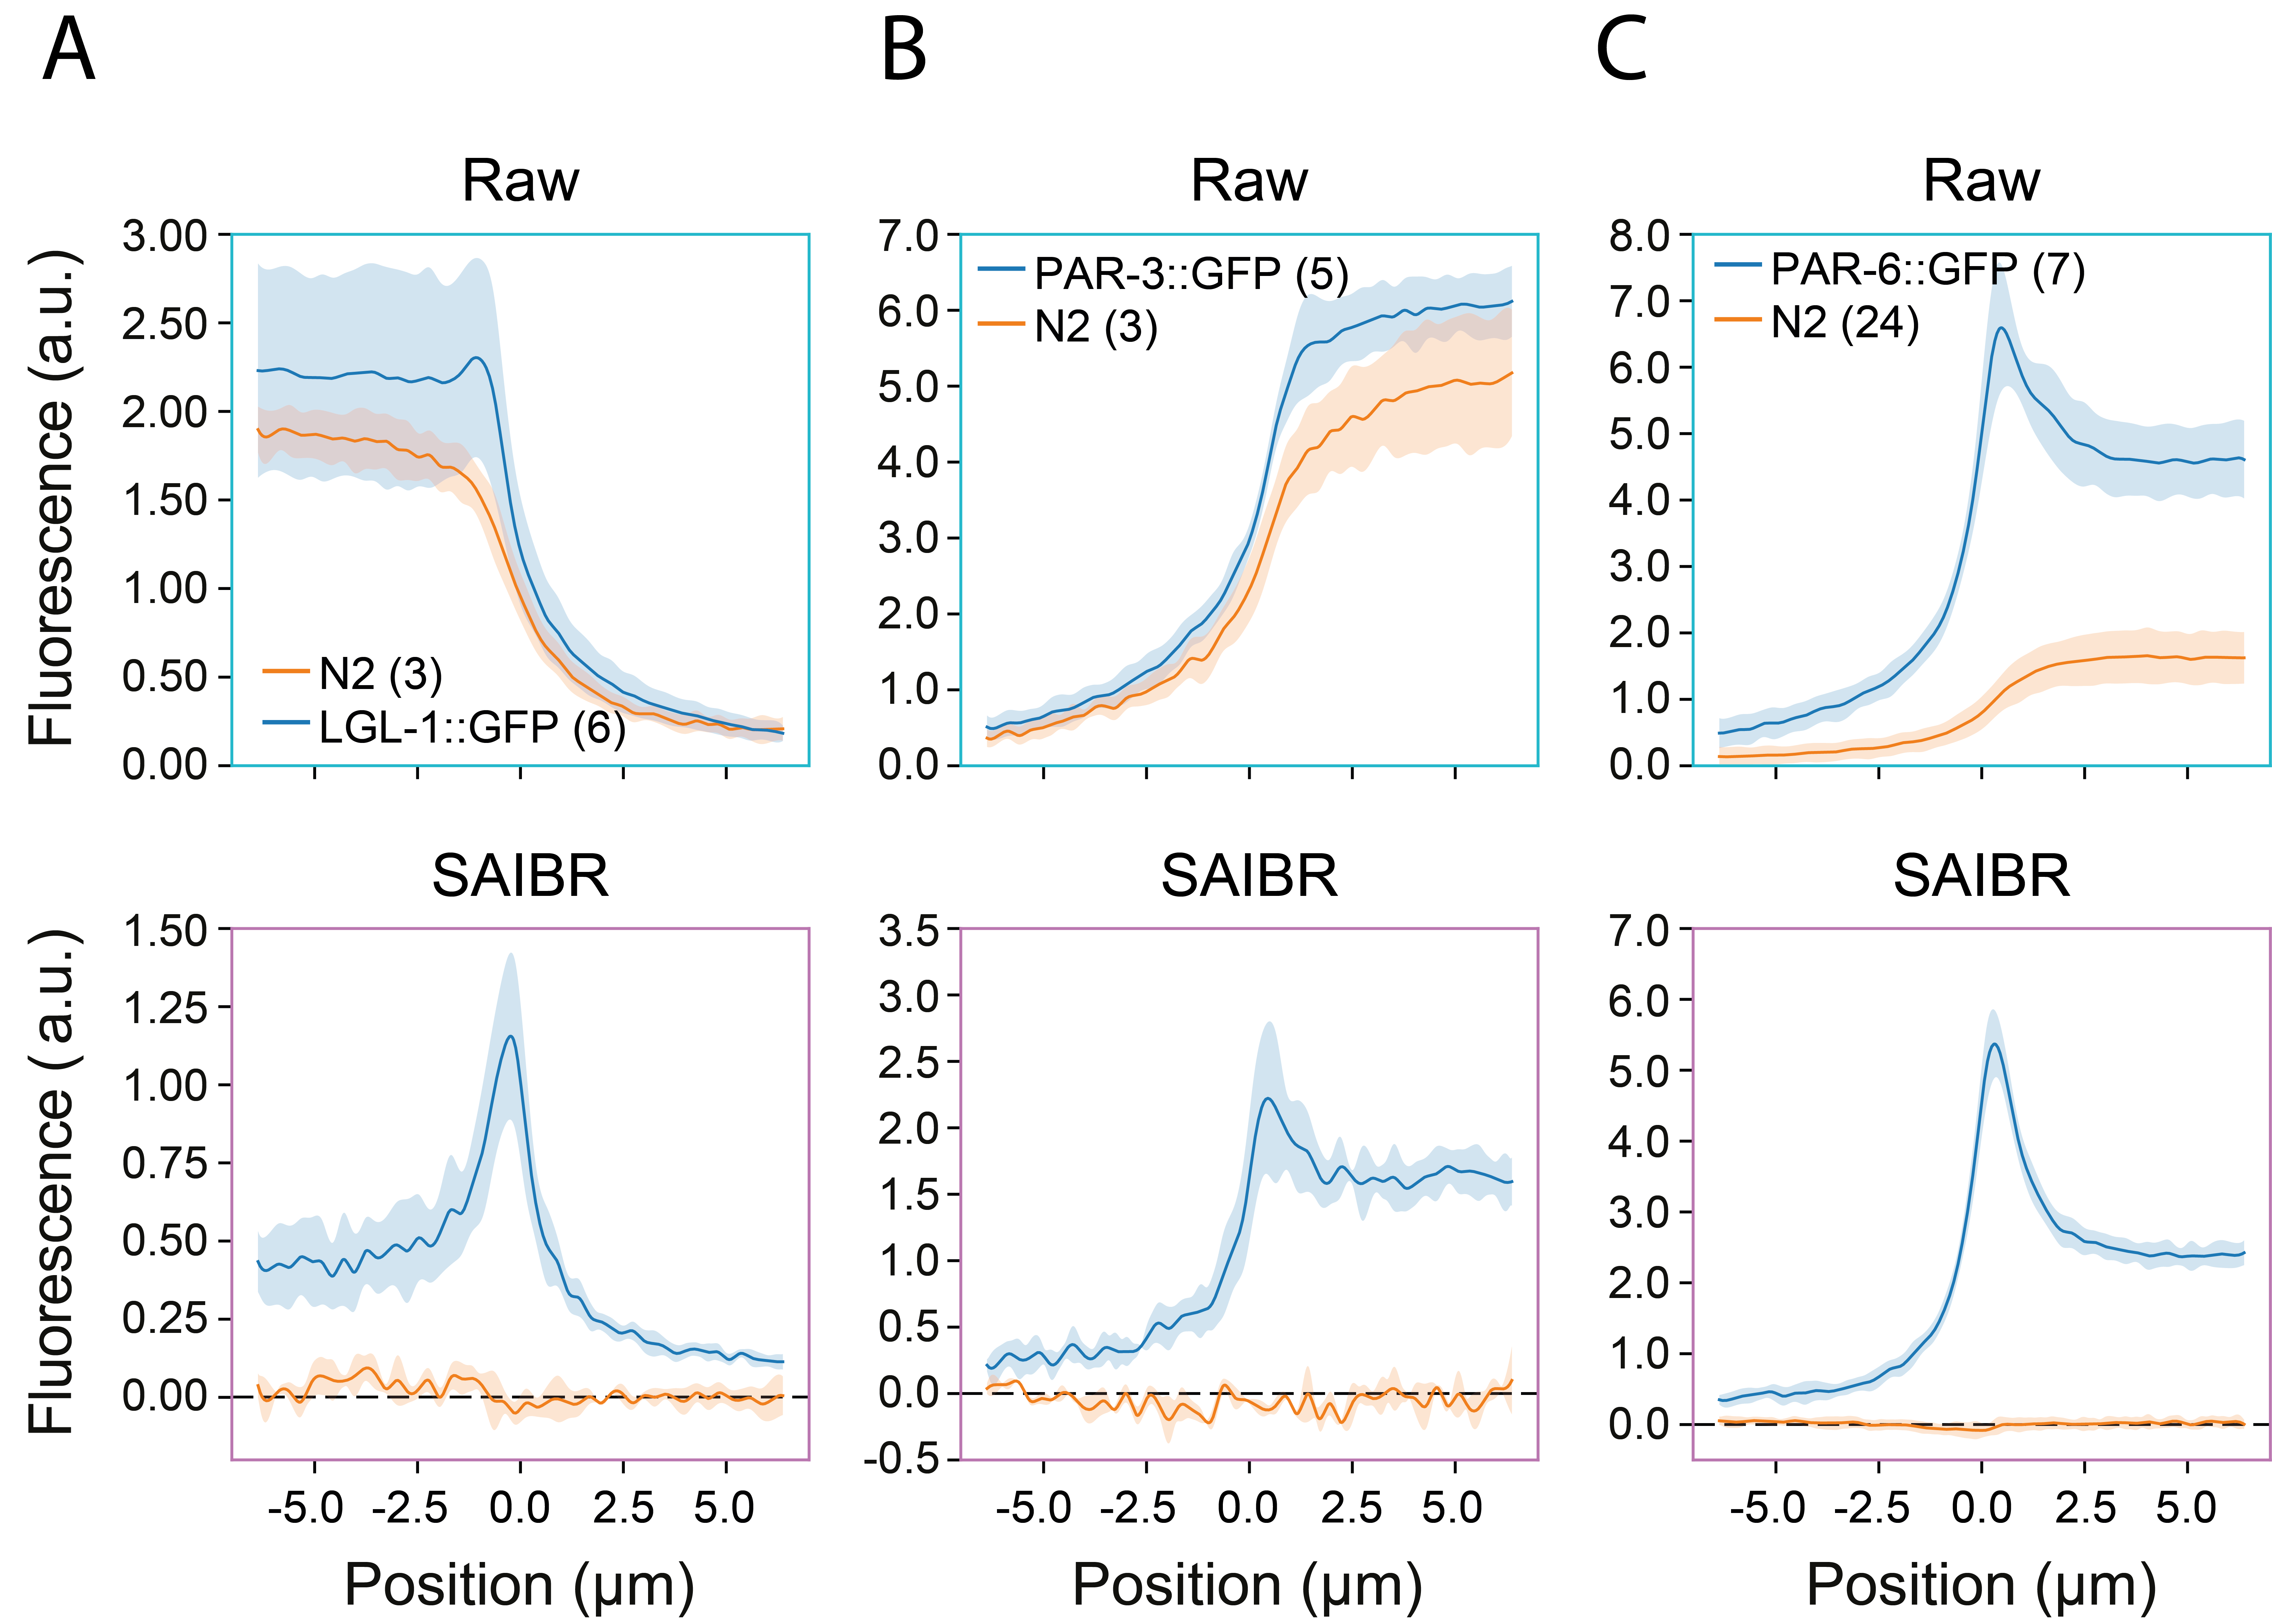
\includegraphics[scale=1]{saibr_membrane_profiles}
\centering
\mycaption{SAIBR improves detection of membrane signals}{
\textbf{(A) - (C)} Averaged membrane profiles taken from raw (top) and SAIBR-corrected (bottom) images for LGL-1::GFP (A), PAR-3::GFP(B) and PAR-6::GFP (C) shown relative to unlabelled N2 controls. Membrane position at x=0$\mu m$. Mean $\pm$ SD indicated.
Fig. 2E-G from \textcite{Rodrigues2022}.}
\label{fig:saibr_membrane_profiles}
\end{figure}

\subsection{Extending SAIBR to dual-labelled \textit{C. elegans} embryos}

As SAIBR relies on a red shifted emission channel, complications can arise in samples containing red fluorophore. As red fluorophores are usually weakly excited by blue lasers, they will contribute additional signal to the AF channel, which may lead to overestimation, and therefore oversubtraction, of autofluorescence if not accounted for. If RFP levels are low, this effect may be small and can be ignored. However, if RFP levels are high, this bleedthrough effect can be significant. This can be demonstrated by observing the inter-channel relationship in control embryos expressing mCh::MEX-5 (\cref{fig:saibr_3channel_correlation}A). We find that, when an RFP is present, this relationship deviates significantly from the typical relationship observed in N2s, in direct proportion to local signal in the RFP (561nm excitation, 630/75nm emission) channel (\cref{fig:saibr_3channel_correlation}A inset). As this relationship is linear, autofluorescence in the GFP channel can be described as a linear function of both the AF and the RFP channels. Plotting pixel data in three dimensions shows that the data can be successfully fit to a plane, by performing multiple linear regression (\cref{fig:saibr_3channel_correlation}B, C). \\


\begin{figure}
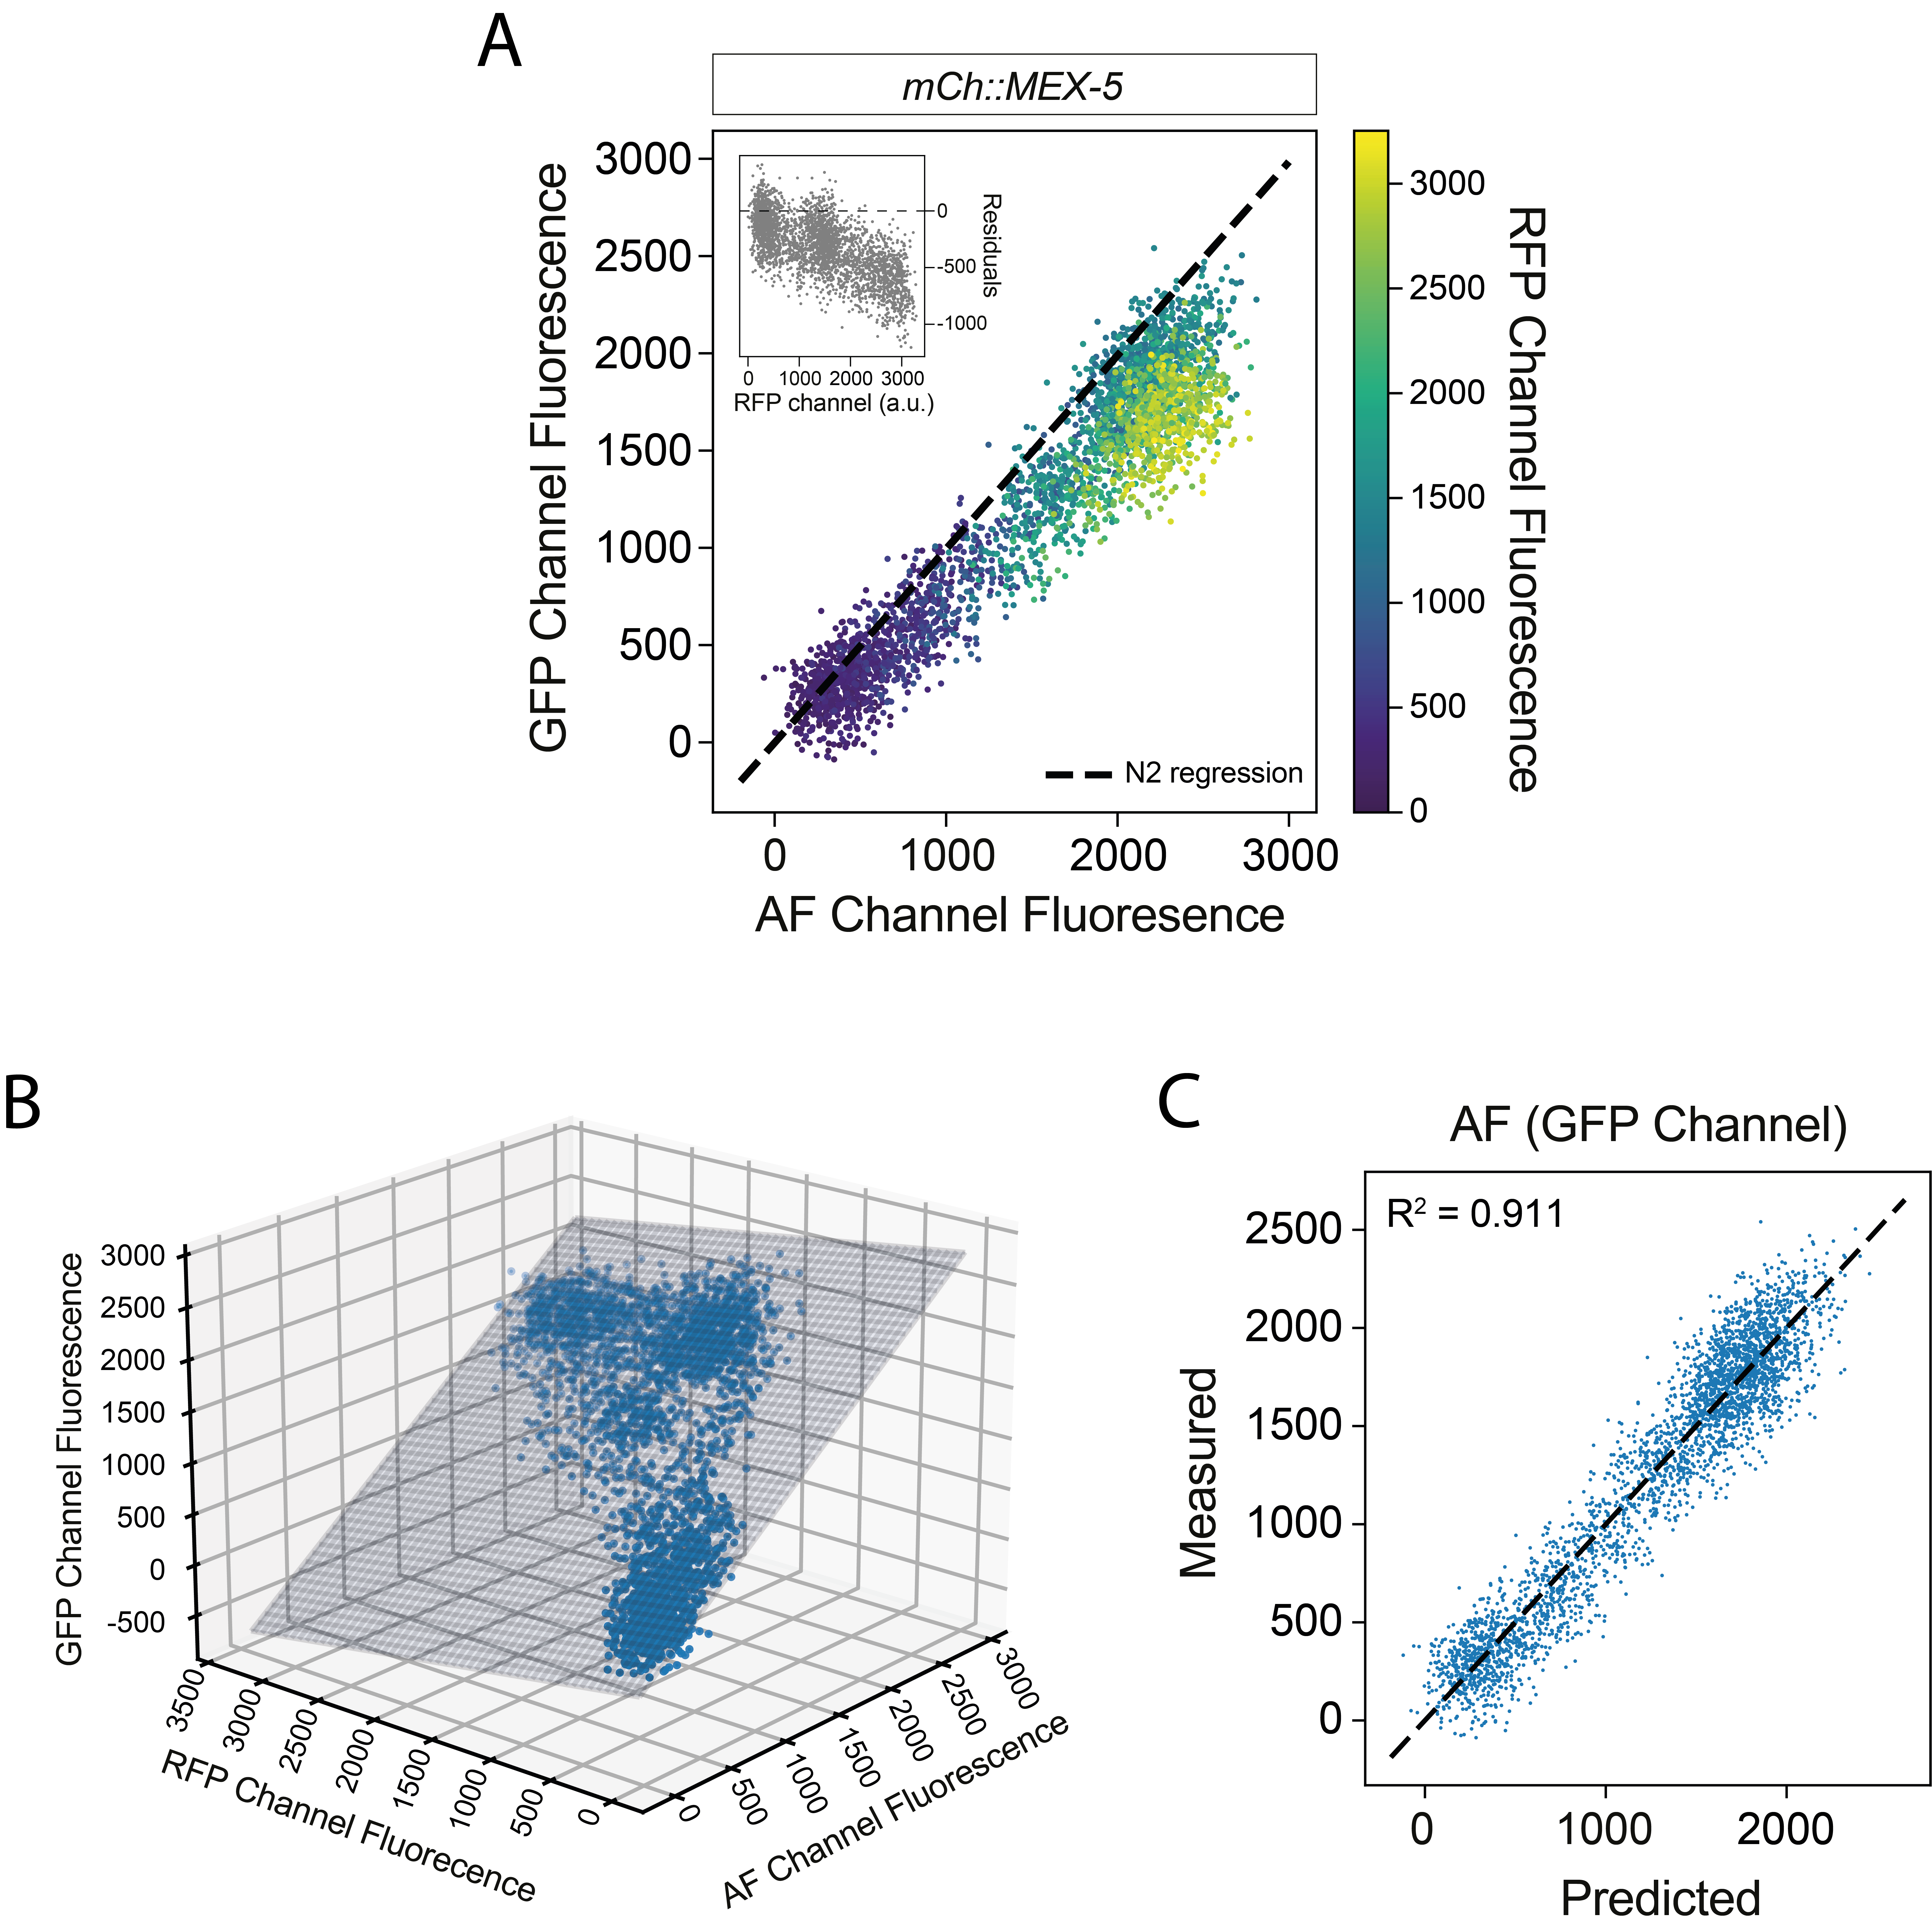
\includegraphics[scale=1]{saibr_3channel_correlation}
\centering
\mycaption{Pixel intensities correlate across three channels in samples containing red fluorophore.}{
\textbf{(A)} Gaussian-filtered (radius = 1) GFP channel vs AF channel pixel intensities for an mCh::MEX-5 expressing embryo, colour coded by RFP-channel fluorescence. Dashed line indicates the AF vs GFP correlation for untagged (N2) embryos. Inset shows residuals as a function of RFP channel signal. Pixels taken from an ROI encompassing the embryo and a region of the background, and 10\% of pixels are shown at random.
\textbf{(B)} Multiple regression fit of GFP-channel signal as a function of AF and RFP channel signal. The same embryo and sample of pixels as in (A) is shown.
\textbf{(C)} Predicted vs. measured GFP-channel signal based on the fit in (B). The same embryo and sample of pixels as in (A) and (B) is shown.
Fig. 4B-D from \textcite{Rodrigues2022}.
}
\label{fig:saibr_3channel_correlation}
\end{figure}

To perform correction on images containing red fluorophore, we just need to capture all three channels, calculate autofluorescence using the three-channel regression relationship obtained from the appropriate RFP-tagged single line, and then subtract this away from the GFP channel image. This is demonstrated in \cref{fig:saibr_3channel_correction}, for embryos expressing both PAR-6::GFP and mCh::MEX-5, or just mCh::MEX-5. Whereas 2-channel SAIBR results in oversubtraction of autofluorescence (particularly visible in the mCh::MEX-5 single line), this is eliminated when using 3-channel SAIBR.\\

\begin{SCfigure}
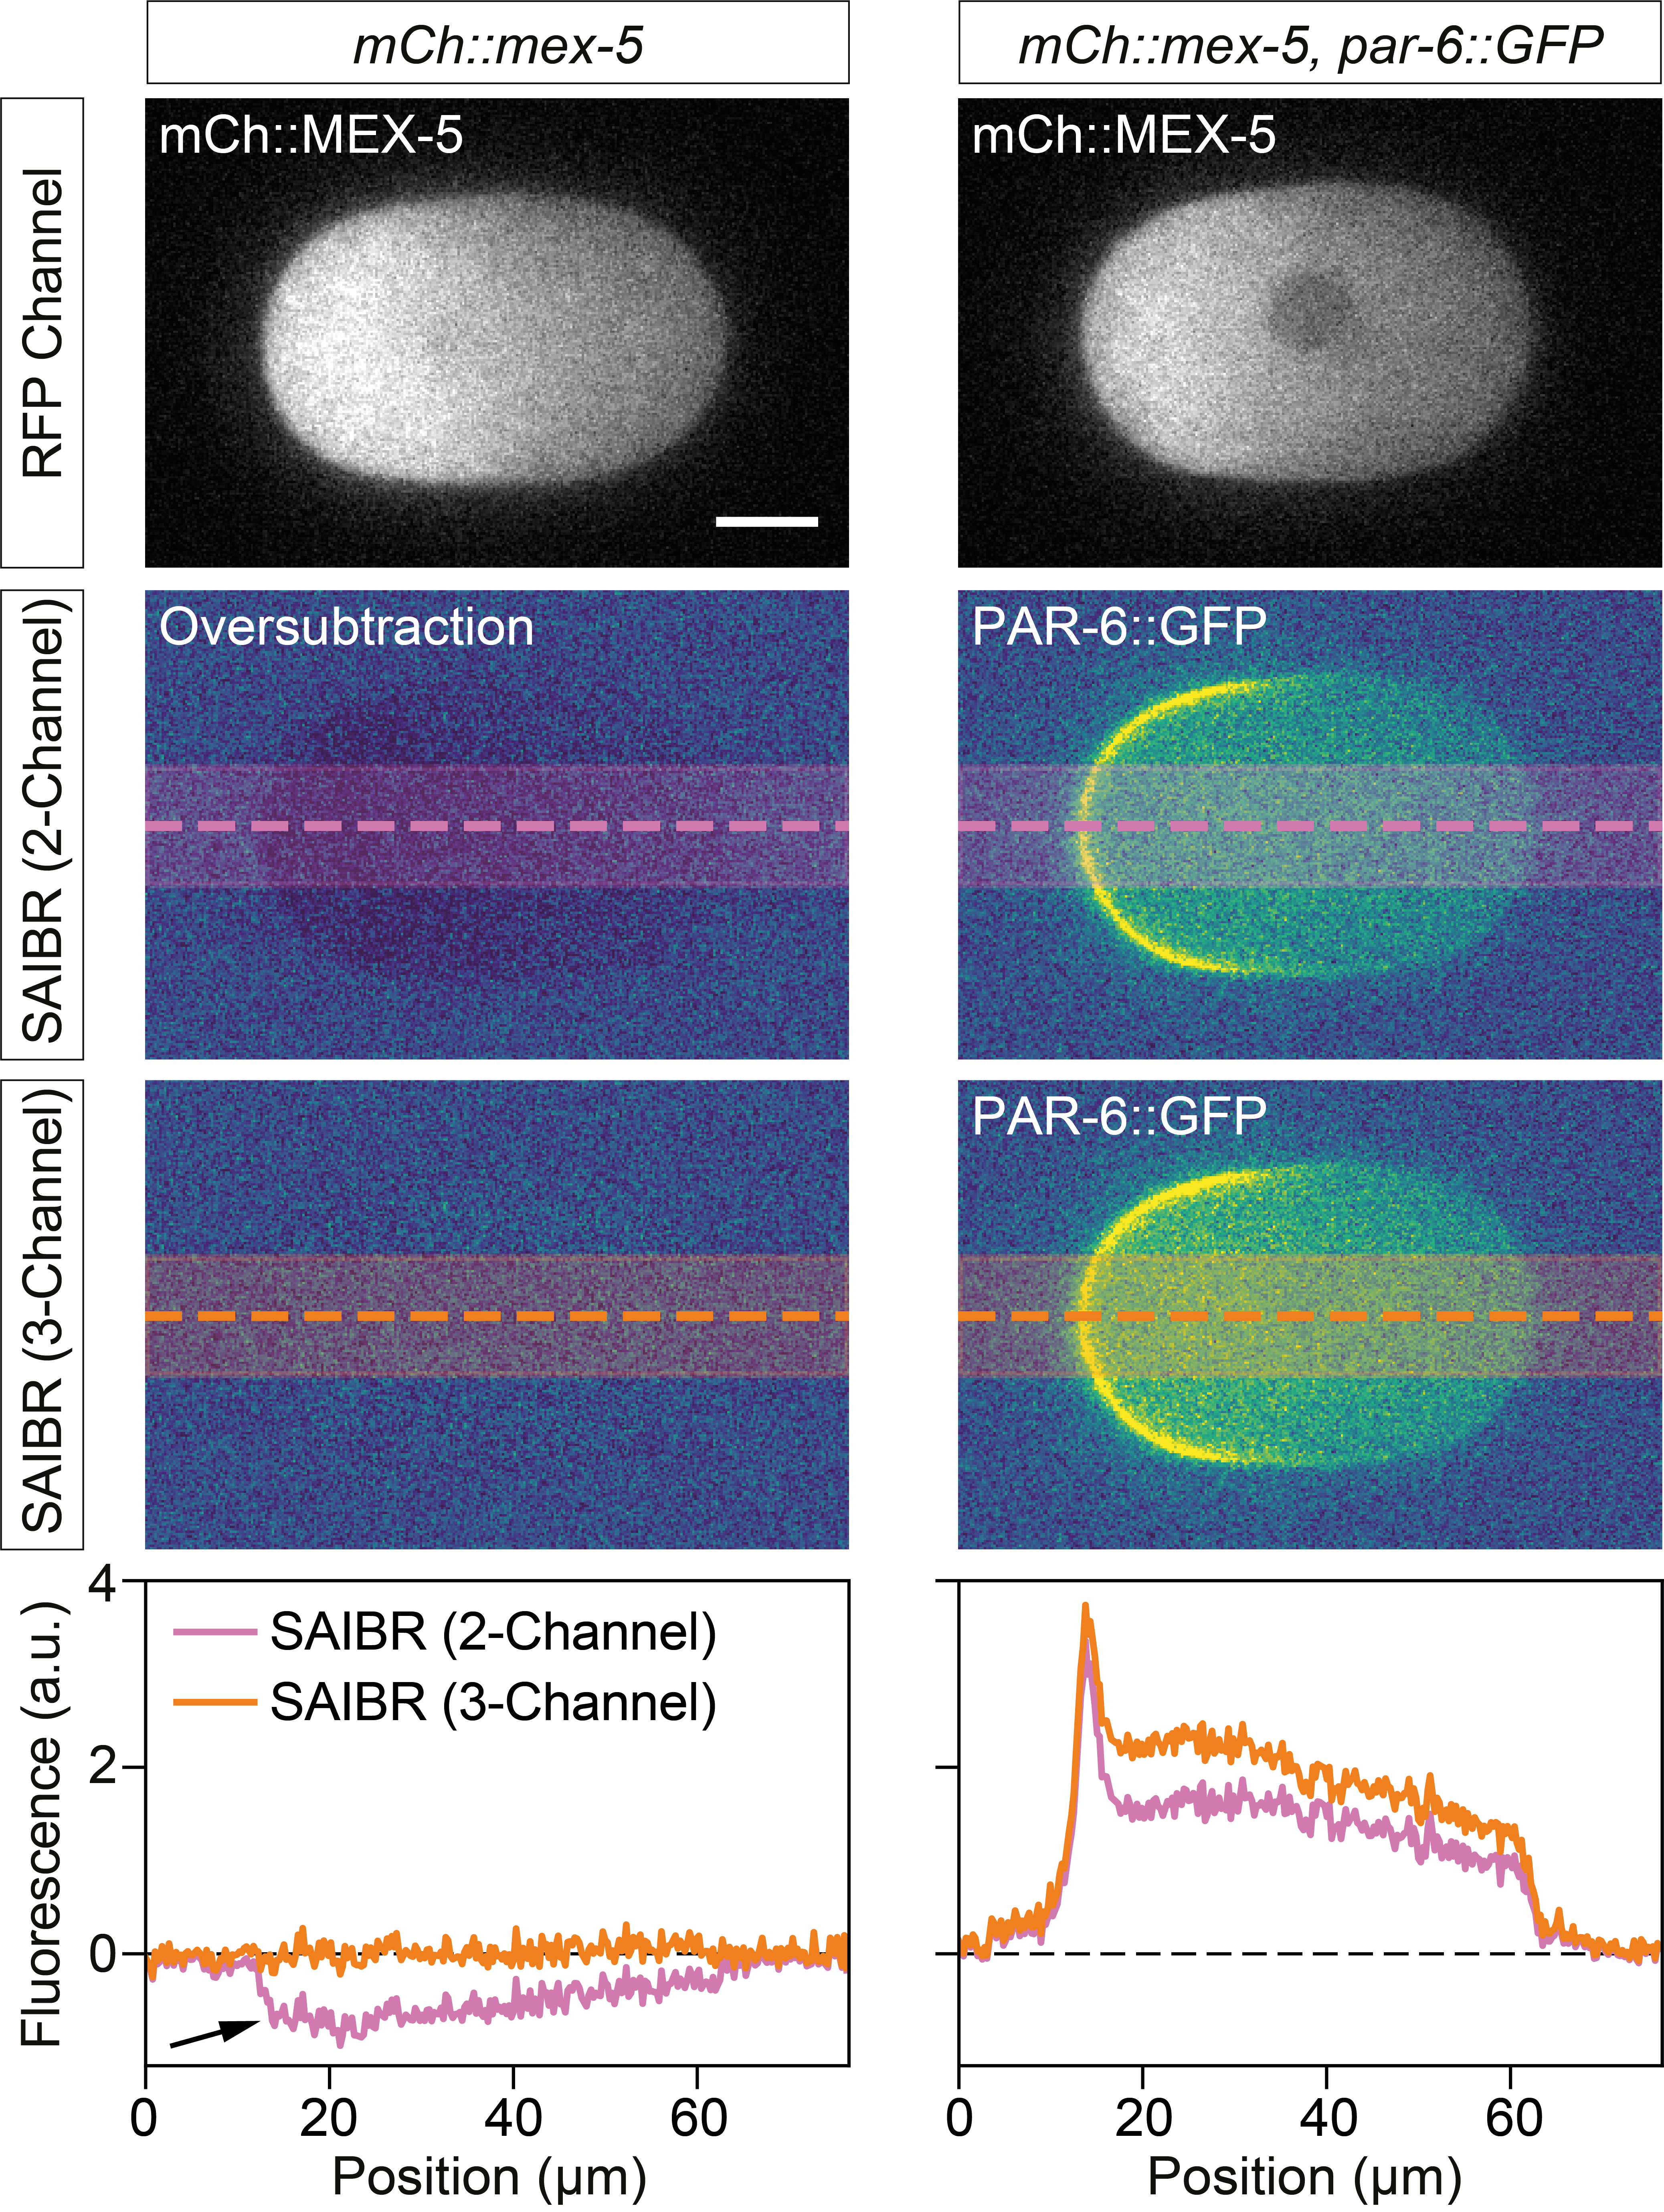
\includegraphics[scale=1]{saibr_3channel_correction}
\mycaption{3-channel SAIBR prevents oversubtraction in samples containing red fluorophore}{
RFP channel, 2-channel SAIBR and 3-channel SAIBR images for samples expressing mCh::MEX-5, along with associated linescans. 2-channel SAIBR results in oversubtraction which is clearly visible as negative values in the mCh::MEX-5 line (arrow) and reduced cytoplasmic signal in the two-colour line. 3-channel SAIBR, using the calibration procedure shown in \cref{fig:saibr_3channel_correlation}, prevents oversubtraction.
Fig. 4F from \textcite{Rodrigues2022}.}
\label{fig:saibr_3channel_correction}
\end{SCfigure}


\subsection{Discussion}

In summary, I have demonstrated that a simple protocol, which we’ve termed SAIBR, can be used to successfully remove autofluorescence in images of \textit{C. elegans} zygotes. The improvements are particularly striking for images of fusion proteins with low levels of expression, such as LGL-1::GFP, but even in cases where expression levels are higher, AF correction will prove important for quantitative analysis of membrane concentrations, as discussed in the next section. For the rest of this thesis, unless otherwise stated, green fluorophore images will be presented with autofluorescence removed by SAIBR.\\

The simplicity of the method means that it can be easily incorporated into existing workflows, and should be applicable to a variety of imaging platforms. In the full study \citep{Rodrigues2022}, we show that the method is equally successful on both spinning-disk confocal and wide-field instruments. \\

Whilst initially developed with \textit{C. elegans} embryos in mind, the method isn't specific to this system, and could be applied to a number of other model systems in which autofluorescence is a problem. In the full study, we show that the method works successfully in \textit{C. elegans} larvae, as well as other model organisms such as starfish and yeast. That said, the method isn’t guaranteed to perform well in all cases. If samples contain multiple, independently varying sources of autoflourescence, then SAIBR may face problems as a single autofluorescence reporter channel cannot account for this. However, much like how we can tackle red fluorophores, we have found that in some cases this can be solved simply by adding one extra reporter channel. Inevitably, though, such an approach may not be compatible with dual-colour imaging. \\

Whilst the analysis steps are relatively straightforward, implementing the computational workflow may still be a barrier to adoption for some. Therefore, to make the protocol accessible, I have put together a simple GUI-based FIJI plugin which can carry out all the necessary analysis in a few simple steps. This can be found here: \url{https://github.com/tsmbland/saibr_fiji_plugin}. \\

The method comes with a few tradeoffs, which will vary in significance depending on the particular study. One issue is that, as the method combines pixel noise from multiple images, corrected images can in some cases be quite noisy, particularly where weak imaging conditions are used. It also requires capturing two emission channels for each image, which doubles sample illumination times and potential phototoxicity, which may be an issue for long timelapses. Additionally, if samples display rapid motion, then the time lag between taking these two channels may lead to pixel mismatches, which could introduce artefacts. These last points could be fixed by using an imaging setup that allows for dual capture of multiple emission bands. However, for this particular study, these issues will not be of major significance. \\


\clearpage
\section{Extracting membrane and cytoplasmic signal components}
\label{section:memquant}

Transition to section

\subsection{An overview of existing methods}

A number of methods have been implemented aiming to quantify protein concentrations at the membrane and cytoplasm in \textit{C. elegans} embryos. A typical approach to quantify membrane concentrations is to find the region of the image representing the cortex (either by manual or computational segmentation) and take a coarse measure of pixel values within this region (\cref{fig:memquant_method_comparison}, \textit{Intensity based quantification}). Such an approach was used by \textcite{Goehring2011a}, who manually segmented the embryo cortex, computationally straightened a region around the circumference of the cell, and defined membrane concentrations as the sum of the highest intensity group of pixels at each cortical cross section. \textcite{Hubatsch2019a} used a similar approach, but replaced manual segmentation with an automated computational pipeline. Similarly, \textcite{Zhang2017} developed a computational protocol to segment images, and defined membrane concentrations around the cell as the average signal intensity within a region representing the cell cortex.\\

\begin{figure}
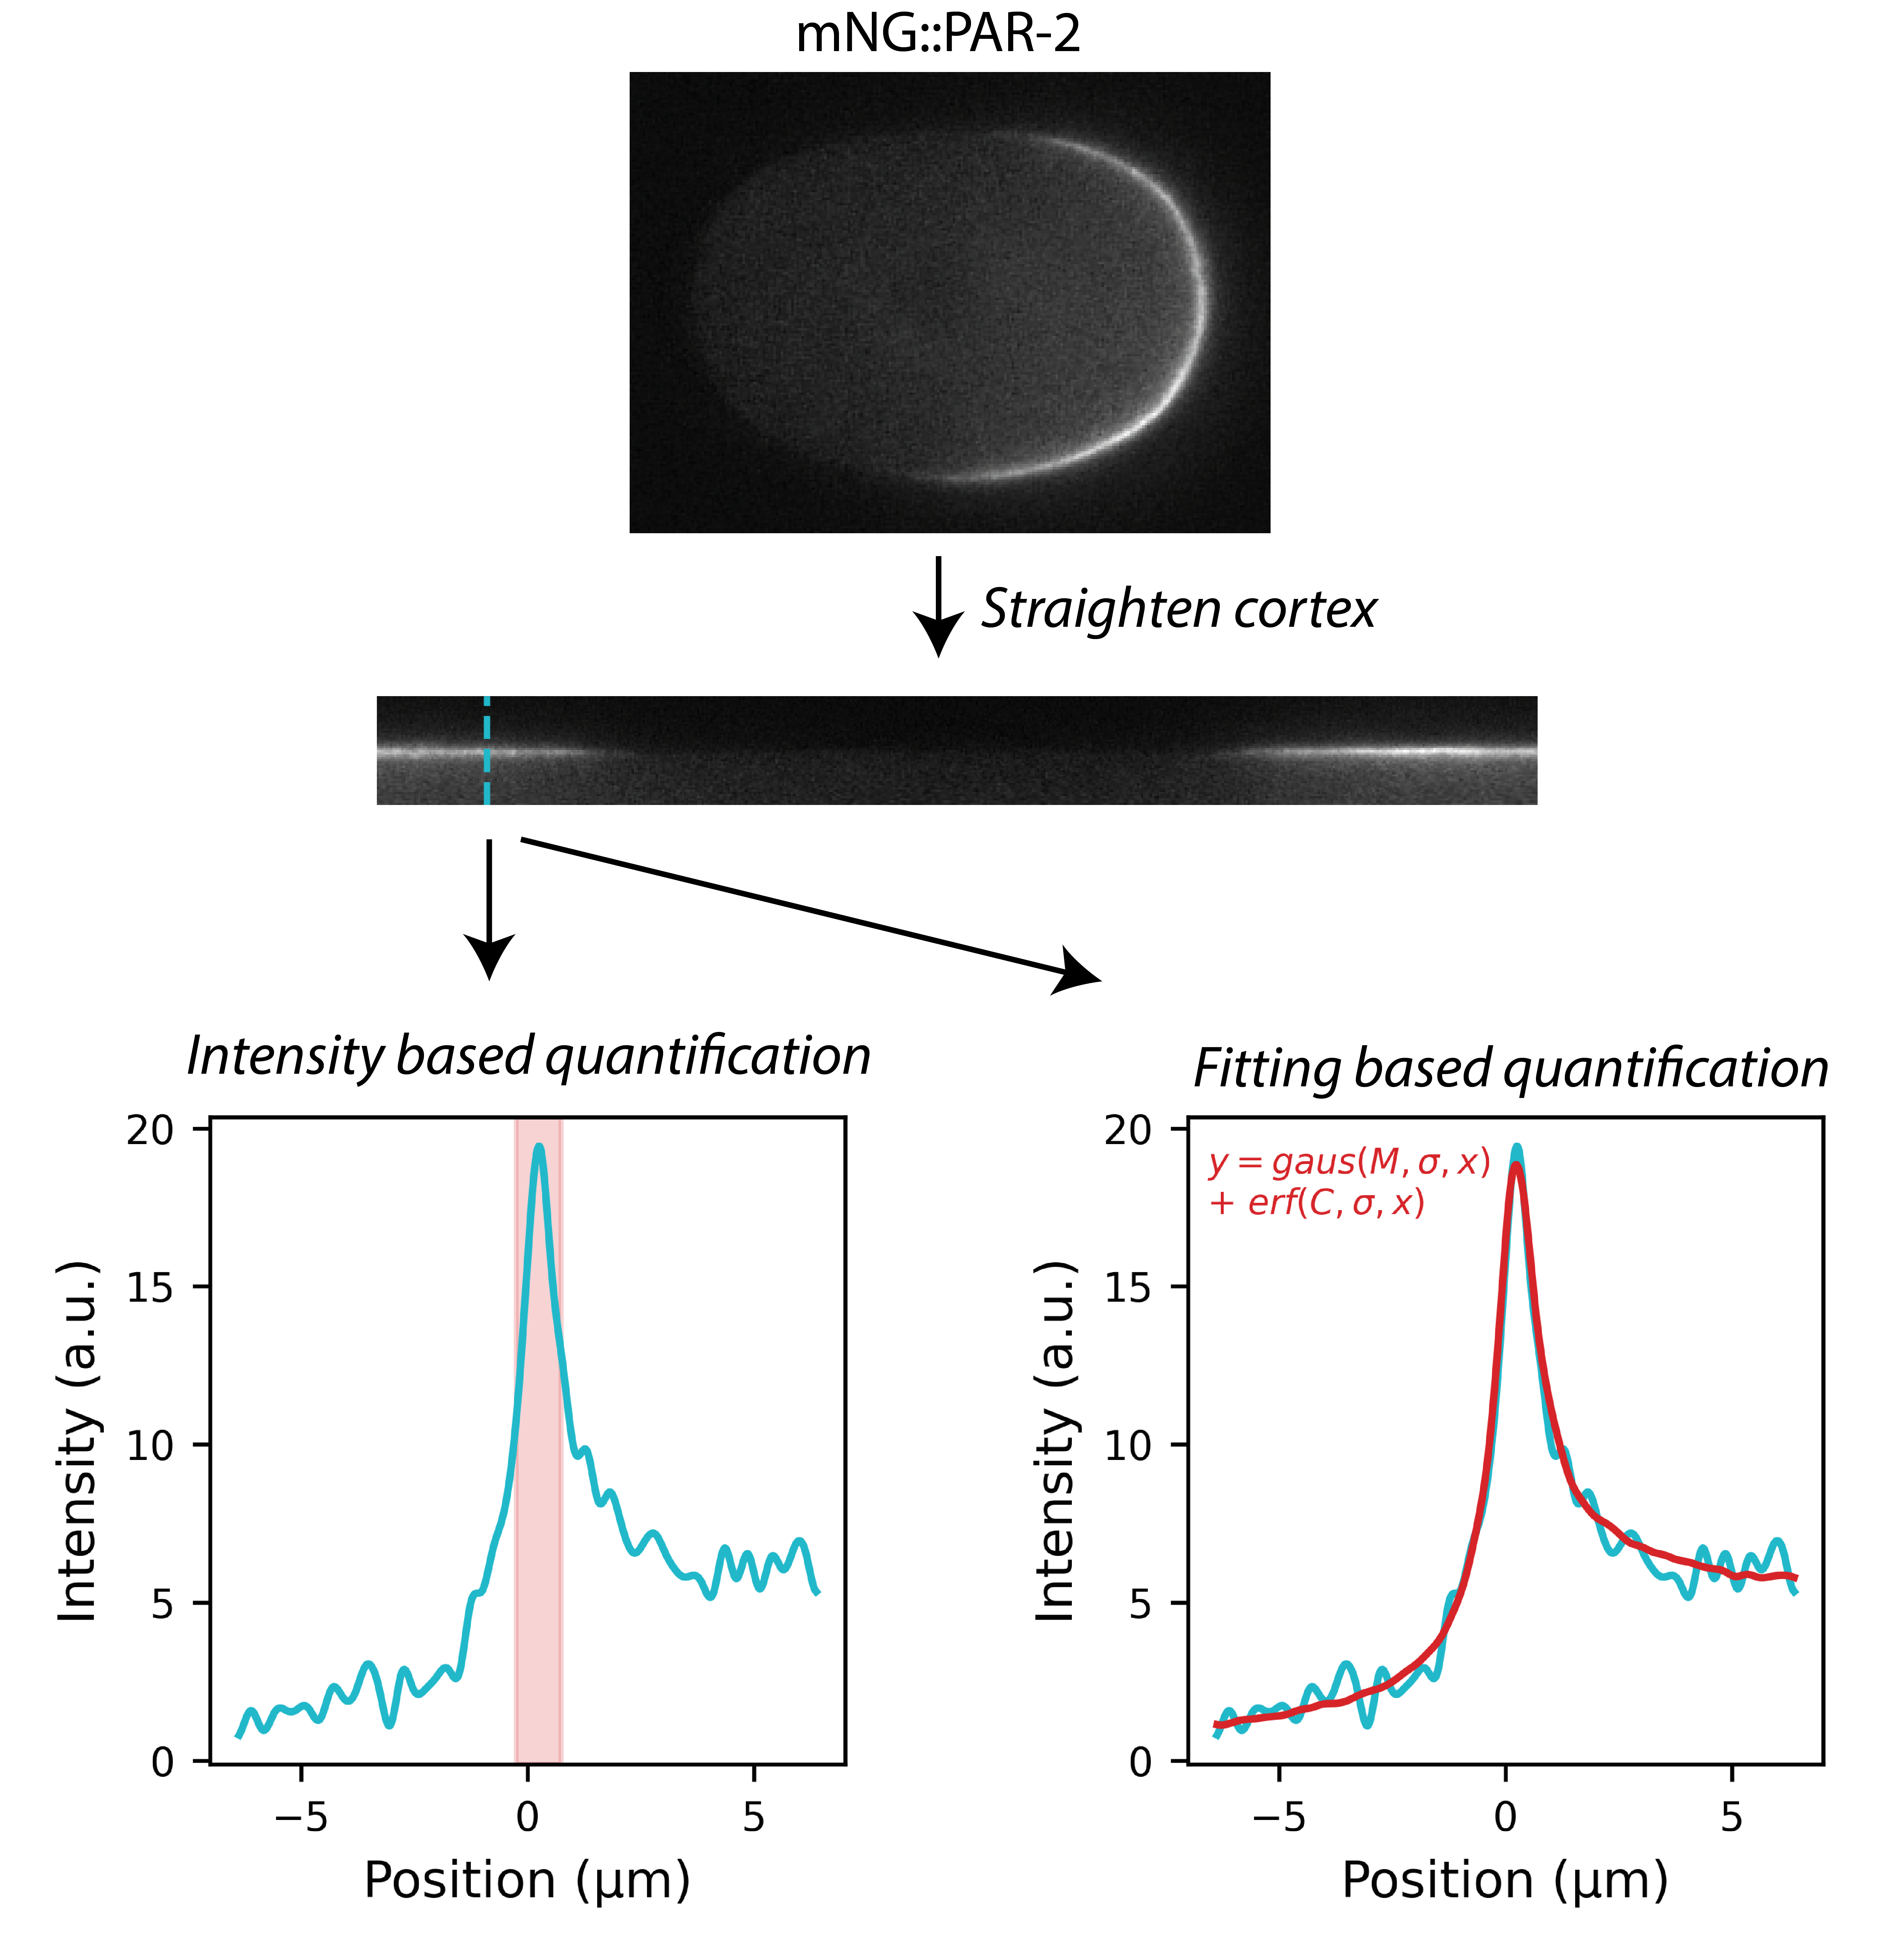
\includegraphics[scale=1]{memquant_method_comparison}
\centering
\mycaption{Approaches for quantifying membrane concentrations from midplane images}{Typical methods involve segmentation of embryos, either manually or computationally, followed by computational straightening, to simplify geometry, here shown for an image of mNG::PAR-2. Each position along the x-dimension of the straightened image represents a profile perpendicular to and centred on the membrane at that position. A number of approaches can be used to extract quantitative information from these profiles. Intensity-based methods use pixel values within a central region of the profile representing the membrane (red) as a measure of membrane concentrations. Fitting-based methods fit the shape of the whole profile to a model, and extract relevant parameters from the fitted model. This is shown here for a model based on \textcite{Gross2018}, which describes total signal as a sum of a Gaussian component representing membrane signal and an error-function component representing cytoplasmic signal. Each component is characterised by an amplitude ($M$ and $C$) and a shared width parameter ($\sigma$).
}
\label{fig:memquant_method_comparison}
\end{figure}

A main disadvantage of these methods is that, as the membrane is immediately apposed to the underlying cytoplasm, pixel values at the membrane will inevitable contain a contribution from cytoplasmic fluorophore signal (and, indeed, cytoplasmic autofluorescence if this isn't accounted for). This means that measurements of membrane concentrations will be sensitive to changes in cytoplasmic concentrations, and means that these methods fail to achieve an accurate zero (a positive signal will always register, even if there is nothing on the membrane). Typically, attempts are made to overcome this latter point by normalising concentrations and/or subtracting away a local or global estimate of the background signal, but this is often difficult and inaccurate.\\

More advanced methods have aimed to overcome this problem by building models to describe the expected shape of individual cross-cortex profiles, based on summed contributions of cytoplasmic and membrane signal. Membrane and cytoplasmic concentrations can then be extracted by fitting measured profiles to this model, and extracting the relevant parameters describing the amplitudes of the two signal components (\cref{fig:memquant_method_comparison}, \textit{Fitting based quantification}). Such an approach was used by \textcite{Gross2018}, who described the cross-cortex profile at each point around the circumference of the embryo as the sum of a Gaussian and an error-function contribution, representing the expected form of a point (membrane) or step-function (cytoplasm) convolved with a Gaussian-like point spread function in 1D. A similar approach was previously used in \textcite{Blanchoud2015} (although with a different description of cytoplasmic signal).\\

\subsection{Accounting for out-of-focus scatter}

Whilst these methods have been effectively deployed in various studies, and are good at capturing a proper zero baseline, their accuracy is inevitably limited by the accuracy of the underlying models. For many imaging set-ups, the assumption that cytoplasmic and membrane contributions can be described by such simple mathematical functions may in fact be far from the truth. This was demonstrated by for \textit{C. elegans} embryos by \textcite{Reich2019a}, who quantitatively analysed cross-cortex signal in cells containing only cytoplasmic signal, finding that (under imaging conditions similar to those used in this study) the shape of this profile deviates significantly from the expected error-function shape. I have also performed similar analysis here  (\cref{fig:memquant_cyt_profile}), in this case using a line expressing free NeonGreen which is not expected to bind to the membrane, and using SAIBR to remove any autofluorescence contributions. Here we can see the true shape of the cytoplasmic signal contribution, which varies little within embryos (\cref{fig:memquant_cyt_profile}C) and between embryos (\cref{fig:memquant_cyt_profile}D).\\

\begin{figure}
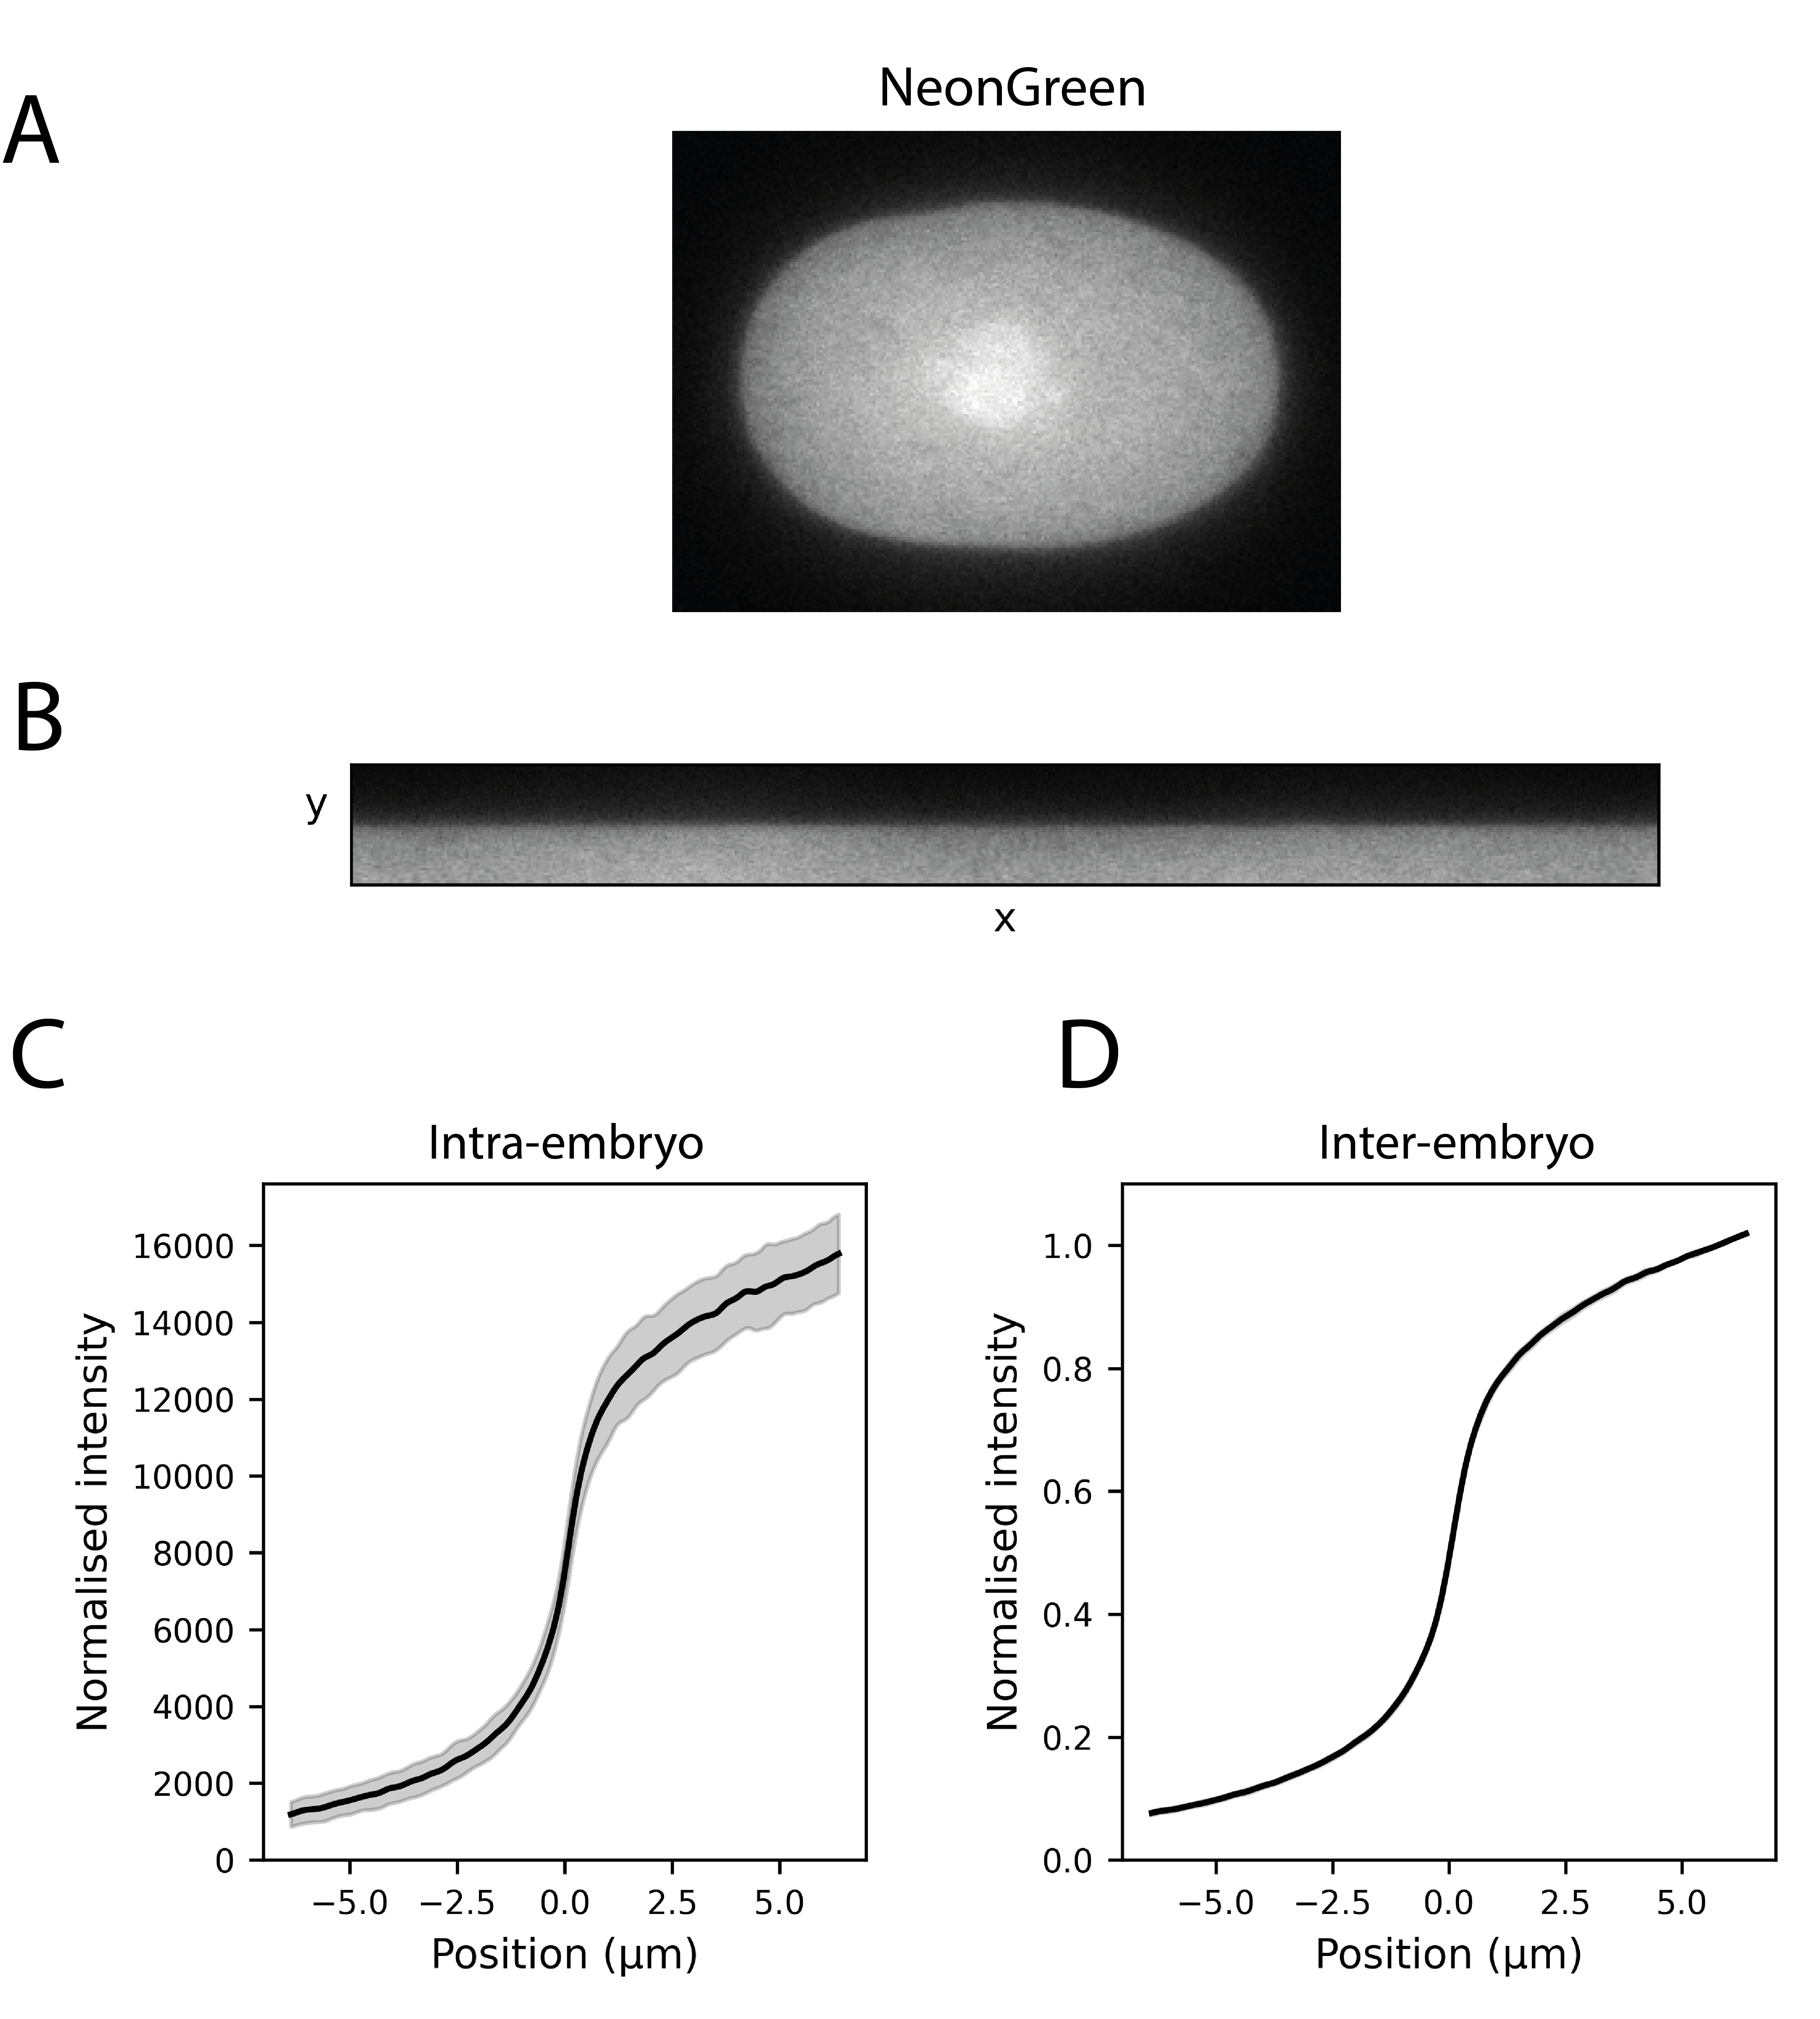
\includegraphics[scale=1]{memquant_cyt_profile}
\centering
\mycaption{Assessing the contribution of cytoplasmic protein to midplane signal}{
\textbf{(A)} Midplane image of an embryo expressing free NeonGreen.
\textbf{(B)} Straightened cortex of the image in (A).
\textbf{(C)} Straightened image in (B), averaged over the x dimension. Mean $\pm$ SD.
\textbf{(D)} Mean ($\pm$ SD) cross-cortex profile, averaged across multiple embryos.
}
\label{fig:memquant_cyt_profile}
\end{figure}

The main reason that this shape deviates from an error-function is likely due to scattering and diffraction of light from planes above and below the imaging plane, combined with a curved geometry in the z-dimension (\cref{fig:memquant_cyt_psf}). Scatter, which is a common issue in images of biological samples, causes a broadening of light in three dimensions as it passes through regions of heterogeneous refractive index. This occurs within the (xy) plane of an image, but is typically far more significant in the z-axis. Whilst confocal microscopes are designed to only capture light from a single plane, the whole sample is illuminated, so they will capture any emitted light from other planes that scatters into the focal plane. This means that pixel intensities within the focal plane will be affected not only by structures within that plane but also structures above and below.\\


\begin{figure}
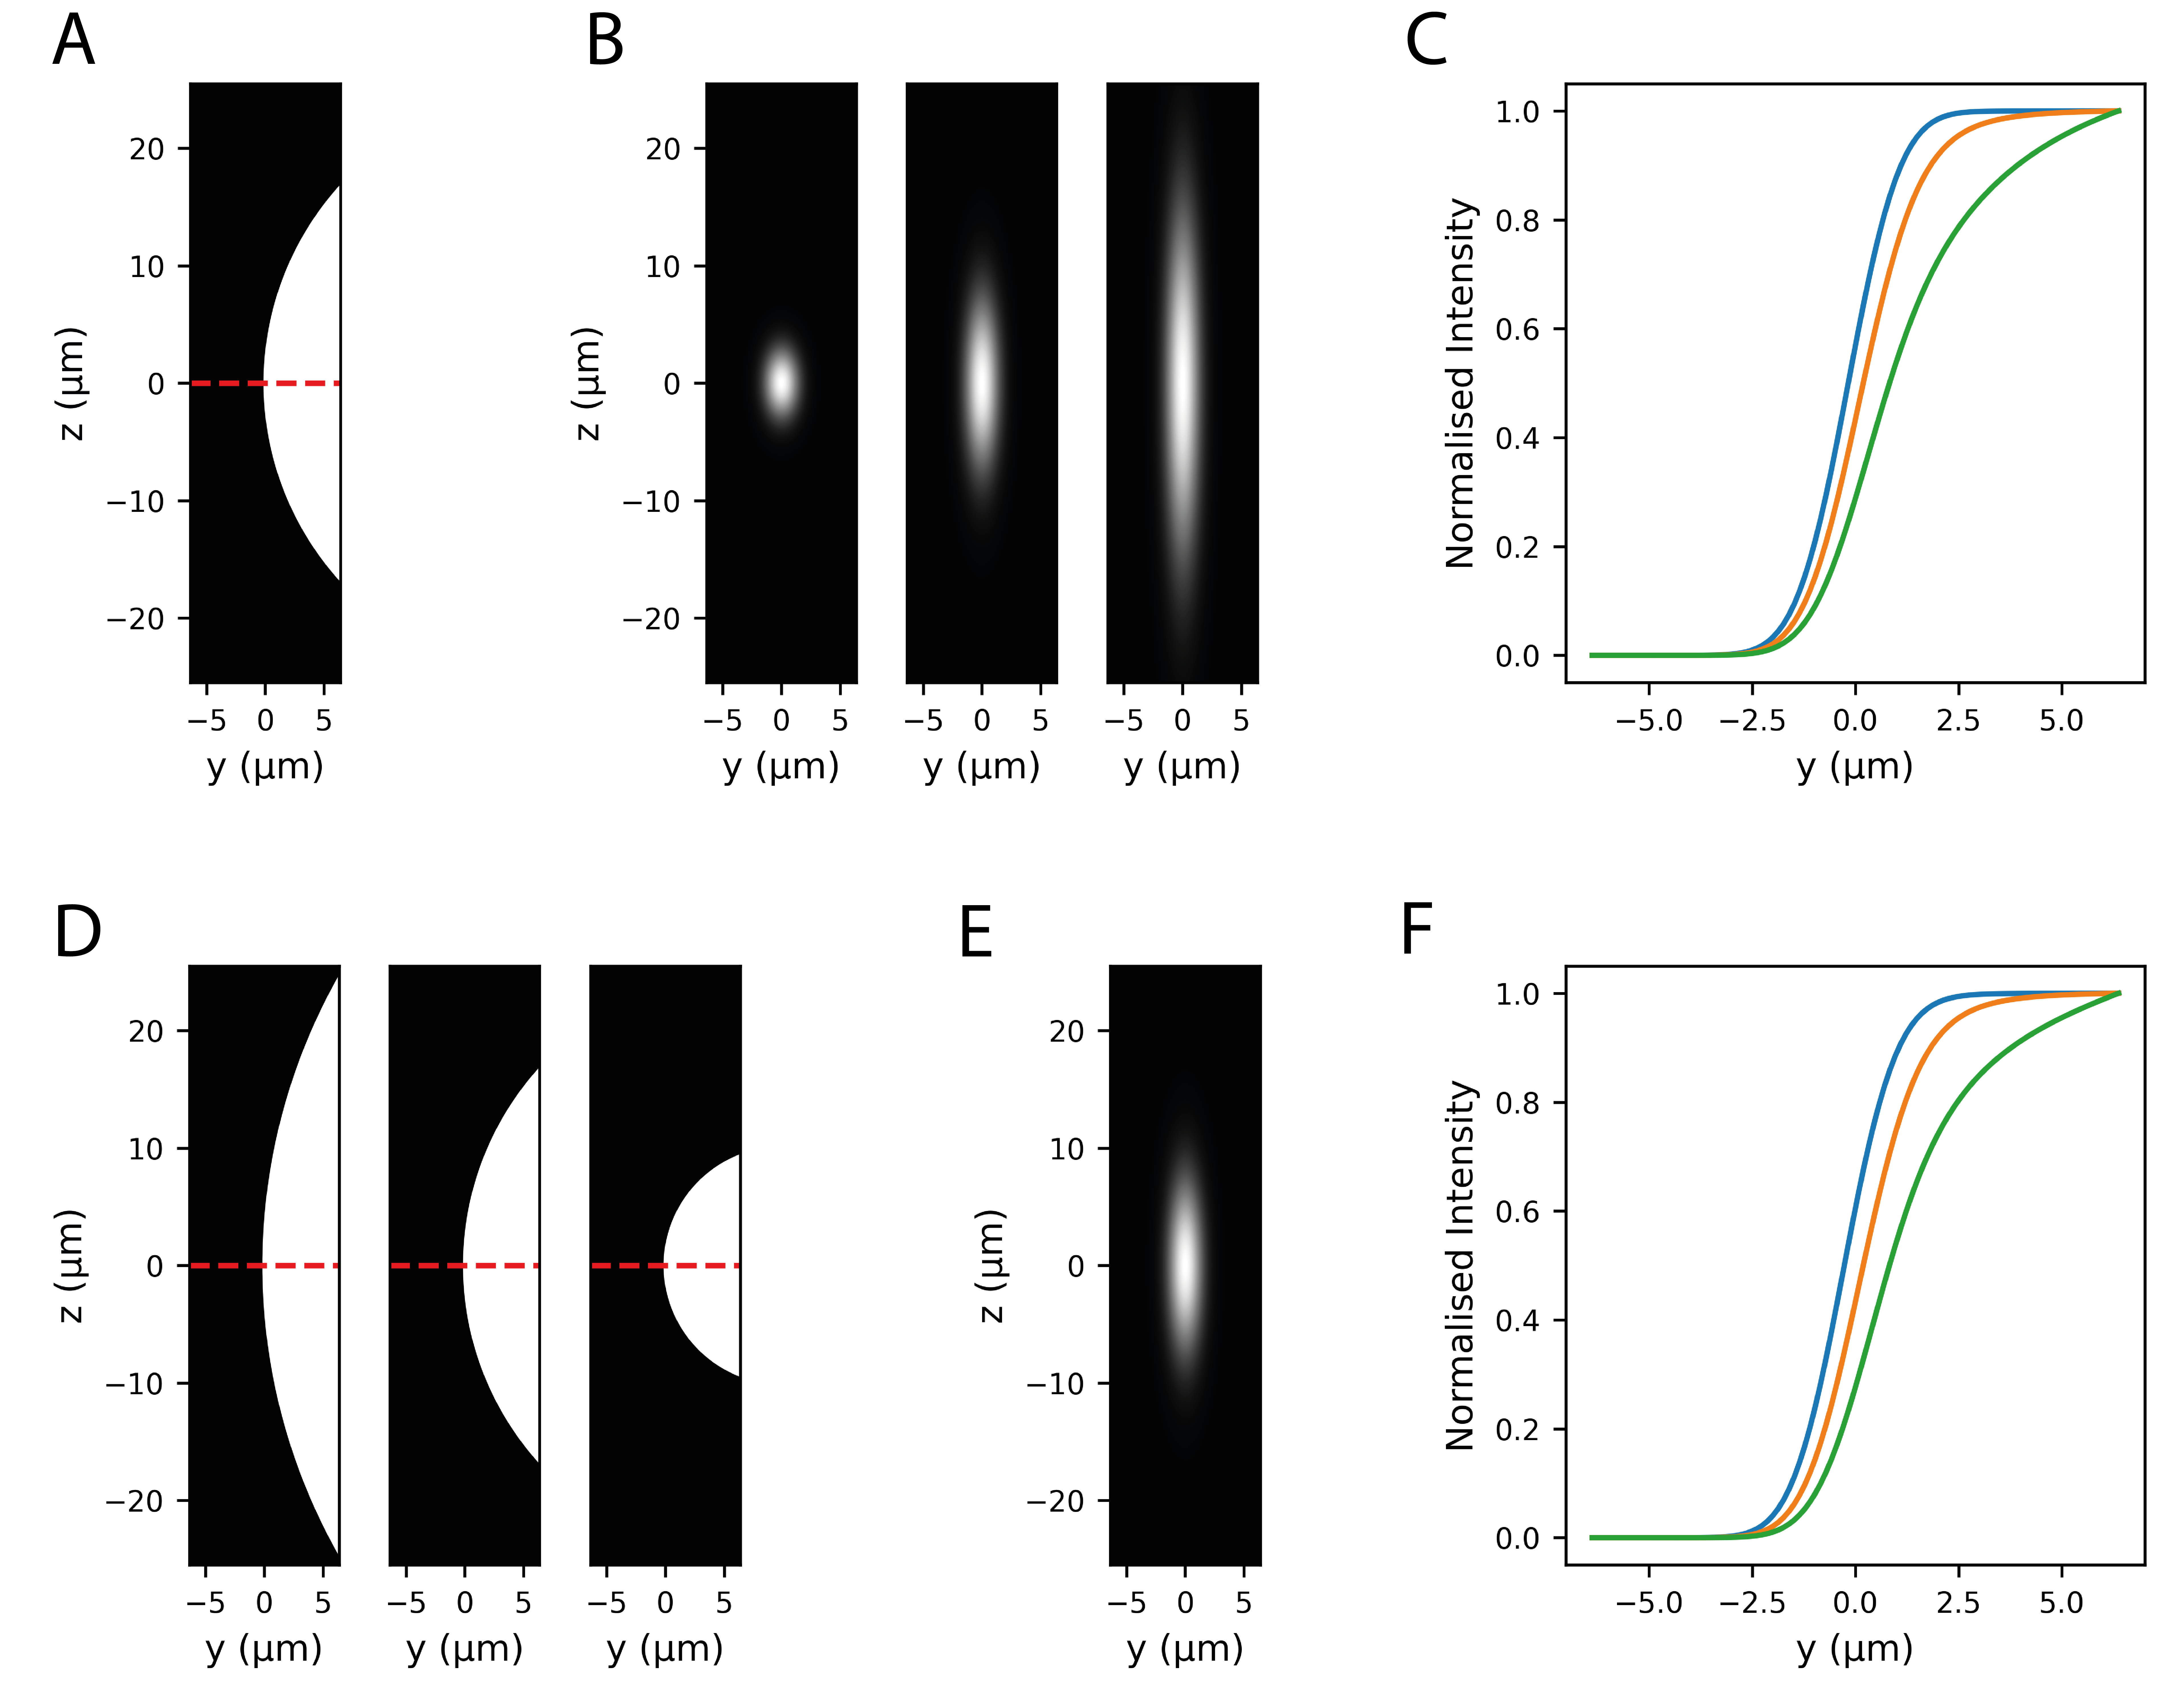
\includegraphics[scale=0.9]{memquant_cyt_psf}
\centering
\mycaption{Effects of sample geometry and the PSF on in-plane signal measurements in simulations of cytoplasm-like signal}{
\textbf{(A) - (C)} (C) shows simulated midplane signals derived from the geometry shown in (A) convolved with three different point spread functions (B).
\textbf{(D) - (F)} (F) shows simulated midplane signals derived from three geometries shown in (D) convolved with the point spread function shown in (E). Geometries are designed to resemble cytoplasmic protein at the edge of a curved cell. Red dashed lines in (A) and (D) indicate midplane. PSFs modelled as 2D Gaussians, which is not representative of real PSFs.
}
\label{fig:memquant_cyt_psf}
\end{figure}

It is likely that a similar problem also applies in the case of membrane protein (\cref{fig:memquant_mem_psf}). Specifically, this analysis shows that out of focus membrane signal might be expected to lead to a shape resembling an asymmetric Gaussian, with higher signal at the interior of the cell than the exterior. In fact, this phenomenon can be observed just by looking at images of polarised PAR proteins (e.g. \cref{fig:memquant_method_comparison} for PAR-2), where out-of-focus membrane signal can create the appearance of a cytoplasmic gradient. By comparison, two-photon images of PAR-2, which aim to eliminate out of focus excitation, show a completely flat cytoplasm \citep{Petrasek2008}, which is expected for most PAR proteins based on fast measured diffusion rates (PAR-3 and PAR-1 excepting). Whilst in some cases this out-of-focus bleedthrough may be of little concern, it might be particularly problematic if accurate cytoplasmic quantification is required, as this out of focus signal may be attributed to cytoplasmic protein. Without accurate cytoplasmic concentration, measures of membrane to cytoplasmic ratios, which are often used as a read-out of membrane affinity, may be wildly off. This will prove significant for much of the analysis in later chapters of this thesis.\\

\begin{figure}
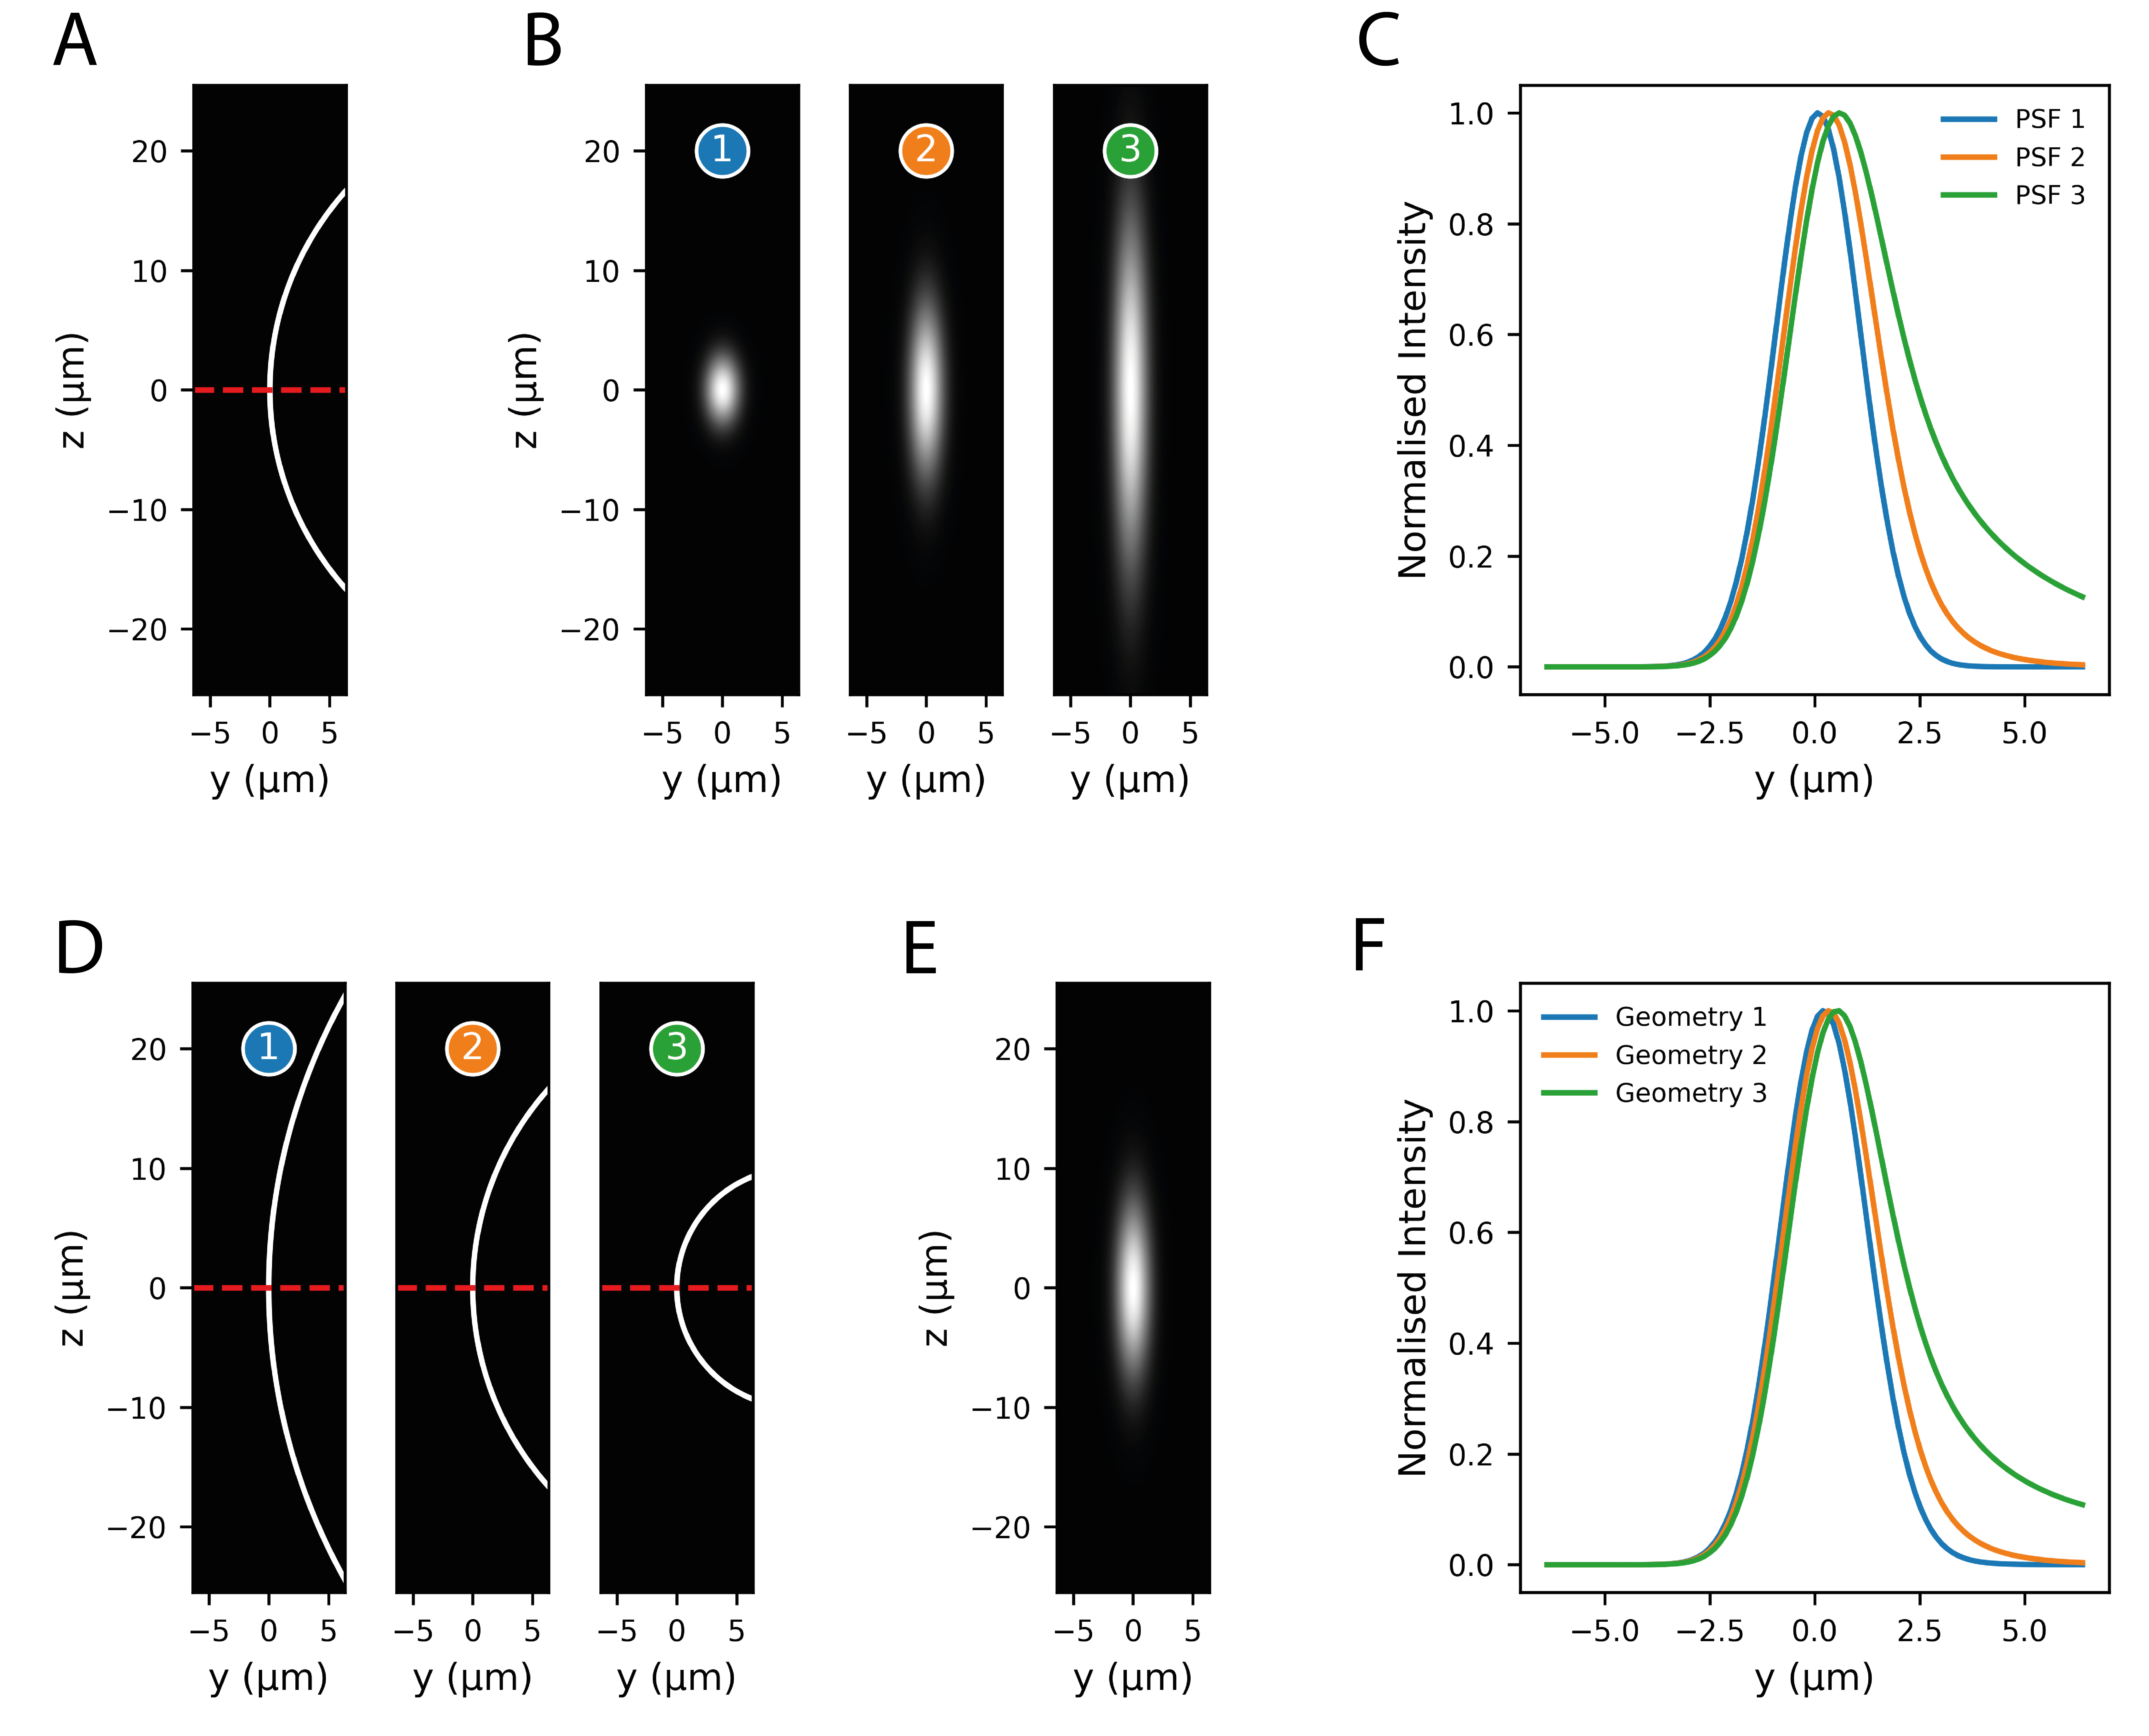
\includegraphics[scale=0.9]{memquant_mem_psf}
\centering
\mycaption{Effects of sample geometry and the PSF on in-plane signal measurements in simulations of membrane-like signal}{
\textbf{(A) - (C)} (C) shows simulated midplane signals derived from the geometry shown in (A) convolved with three different point spread functions (B).
\textbf{(D) - (F)} (F) shows simulated midplane signals derived from three geometries shown in (D) convolved with the point spread function shown in (E). Geometries are designed to resemble membrane protein at the edge of a curved cell. Red dashed lines in (A) and (D) indicate midplane. PSFs modelled as 2D Gaussians, which is not representative of real PSFs.
}
\label{fig:memquant_mem_psf}
\end{figure}

Thus, if we want to obtain accurate measures of cytoplasmic and membrane protein concentrations, we need a method that can account for out-of-focus scatter. One common approach to account for out-of-focus scatter is to take a z-stack across the whole sample and apply a deconvolution algorithm to the 3D stack to reassign all blurred/scattered light to an in-focus location \citep{Wallace2001}. These methods rely on prior knowledge of the point spread function (PSF) that applies to the particular sample and imaging set-up, which needs to be as accurate as possible, otherwise artefacts can arise. Theoretical methods exist to estimate an appropriate PSF given parameters such as the imaging modality, numerical aperture and emitted light wavelength. However, whilst these methods are good at describing blur within the imaging apparatus, scattering within the sample and at the sample-apparatus interface is difficult to model accurately. For this reason, it can be more effective to measure an empirical PSF by imaging the 3D light distribution from a single point source (e.g. a fluorescent bead) under similar sample prep conditions to the sample of interest. However, as PSFs are influenced by scatter within the sample itself, the accuracy of this method depends on how closely the sample environment can be replicated when imaging the beads, which is not trivial. \\

Furthermore, most deconvolution methods assume that the PSF is a constant function throughout the whole image, but in many cases this won't be the case. There may, for example, be refractive index gradients within the sample, which will alter the shape of the PSF depending on location within the sample. Additionally, if there is a mismatch between the refractive index of the immersion and mounting media, as is often unavoidable when imaging live biological samples, then the PSF will usually vary with depth as spherical aberrations will be introduced deeper into the sample. A PSF from a fluorescent bead located directly below the coverslip will not capture either of these phenomena.\\

In reality, given all of these confounding factors, an accurate description of the PSF that applies to a given sample of interest is often unachievable in practice. Whilst deconvolution with a suboptimal PSF may be sufficient for many qualitative applications, accurate quantitative measurements cannot be guaranteed. For this reason, I opted against using a PSF-based deconvolution approach to account for out-of-plane scattering.\\

Fortunately, in this particular case, matters are simplified by the fact that the geometries of protein distribution are usually highly consistent. Not only is the shape of embryos highly consistent, but PAR protein distributions within the embryo also tend to display rotational symmetry (at least during normal polarity development in P0), meaning that protein distributions in planes above and below the focal plane tend to be similar/identical to those seen at the focal plane (much like the simulations in \cref{fig:memquant_cyt_psf} and \cref{fig:memquant_mem_psf}). Optical properties are also not expected to change from sample to sample, or from location to location around the circumference of an embryo.\\

Together, these features imply that, in cases where protein is either entirely cytoplasmic or entirely membrane-bound, the normalised shape of the cross-cortex profile measured at the midplane should be some constant function, that shouldn't vary much between embryos or spatially around the circumference of an embryo. A change in local or global concentrations should amount to a rescaling of these profiles, but shouldn't change their normalised shape. Where there is a mix of cytoplasmic and membrane protein, the total measured cross-cortex profile will then be a sum of these two contributions. Therefore, if one has prior knowledge of the expected shape of the cross-cortex profile for cytoplasmic-only and membrane-only protein, then measured profiles can be fit as the sum of these two contributions, and membrane/cytoplasmic concentrations extracted as the amplitudes of the two signal components.\\

Therefore, a key step in the path to accurate quantification is the ability to measure appropriate reference profiles describing the contributions of cytoplasmic and membrane protein. As mentioned previously, cytoplasmic reference profiles can easily be obtained by analysing cells in which all protein is cytoplasmic (\cref{fig:memquant_cyt_profile}). \textcite{Reich2019a} (and \textcite{Reich2019}) used an approach half-way between the \textcite{Gross2018} method and the method that I am proposing, replacing the error-function description of cytoplasmic signal with a measured cytoplasmic reference profile. Thus, total signals were fit as the sum of a Gaussian profile and this reference profile, which resulted in a better ability of the model to fit the shape of measured profiles.\\

Whilst this move is a significant step in the right direction, the problem remains of how best to account for out of focus membrane light. This presents a challenge: whilst it is relatively easy to directly measure a cytoplasmic reference profile (you just need a reference image in which all signal is cytoplasmic), the same is not true for a membrane profile as it is difficult to find a reference case in which all protein is membrane bound. To extend the method to account for out-of-focus membrane protein, I attempted to find alternative methods to get an approximation of the membrane reference profile. An initial idea, which involved staining the exterior of the embryo eggshell with a fluorescent dye, proved technically challenging and not reproducible.\\

Instead, the problem becomes simplified when one considers that, even in cases where the membrane is polarised, the cytoplasmic pool of most PAR proteins should be uniform (although exceptions do exist in the case of PAR-1 and PAR-3, where true cytoplasmic gradients have been observed). Thus, straightened cortices can be modelled as a uniform cytoplasmic component, defined by a cytoplasmic reference profile ($R_c$) and a single, uniform, cytoplasmic concentration ($C$), plus a polarised membrane component, defined by a membrane reference profile ($R_m$) and a nonuniform membrane concentration profile ($M$), as shown in \cref{fig:memquant_model_schematic}. This is essentially a generalisation of the \textit{Fitting based quantification} method presented in \cref{fig:memquant_method_comparison}, but proposes the use of arbitrary membrane and cytoplasmic reference profiles rather than mathematical functions (e.g. Gaussian, error function), and has the restriction of a uniform cytoplasm.\\

\begin{figure}
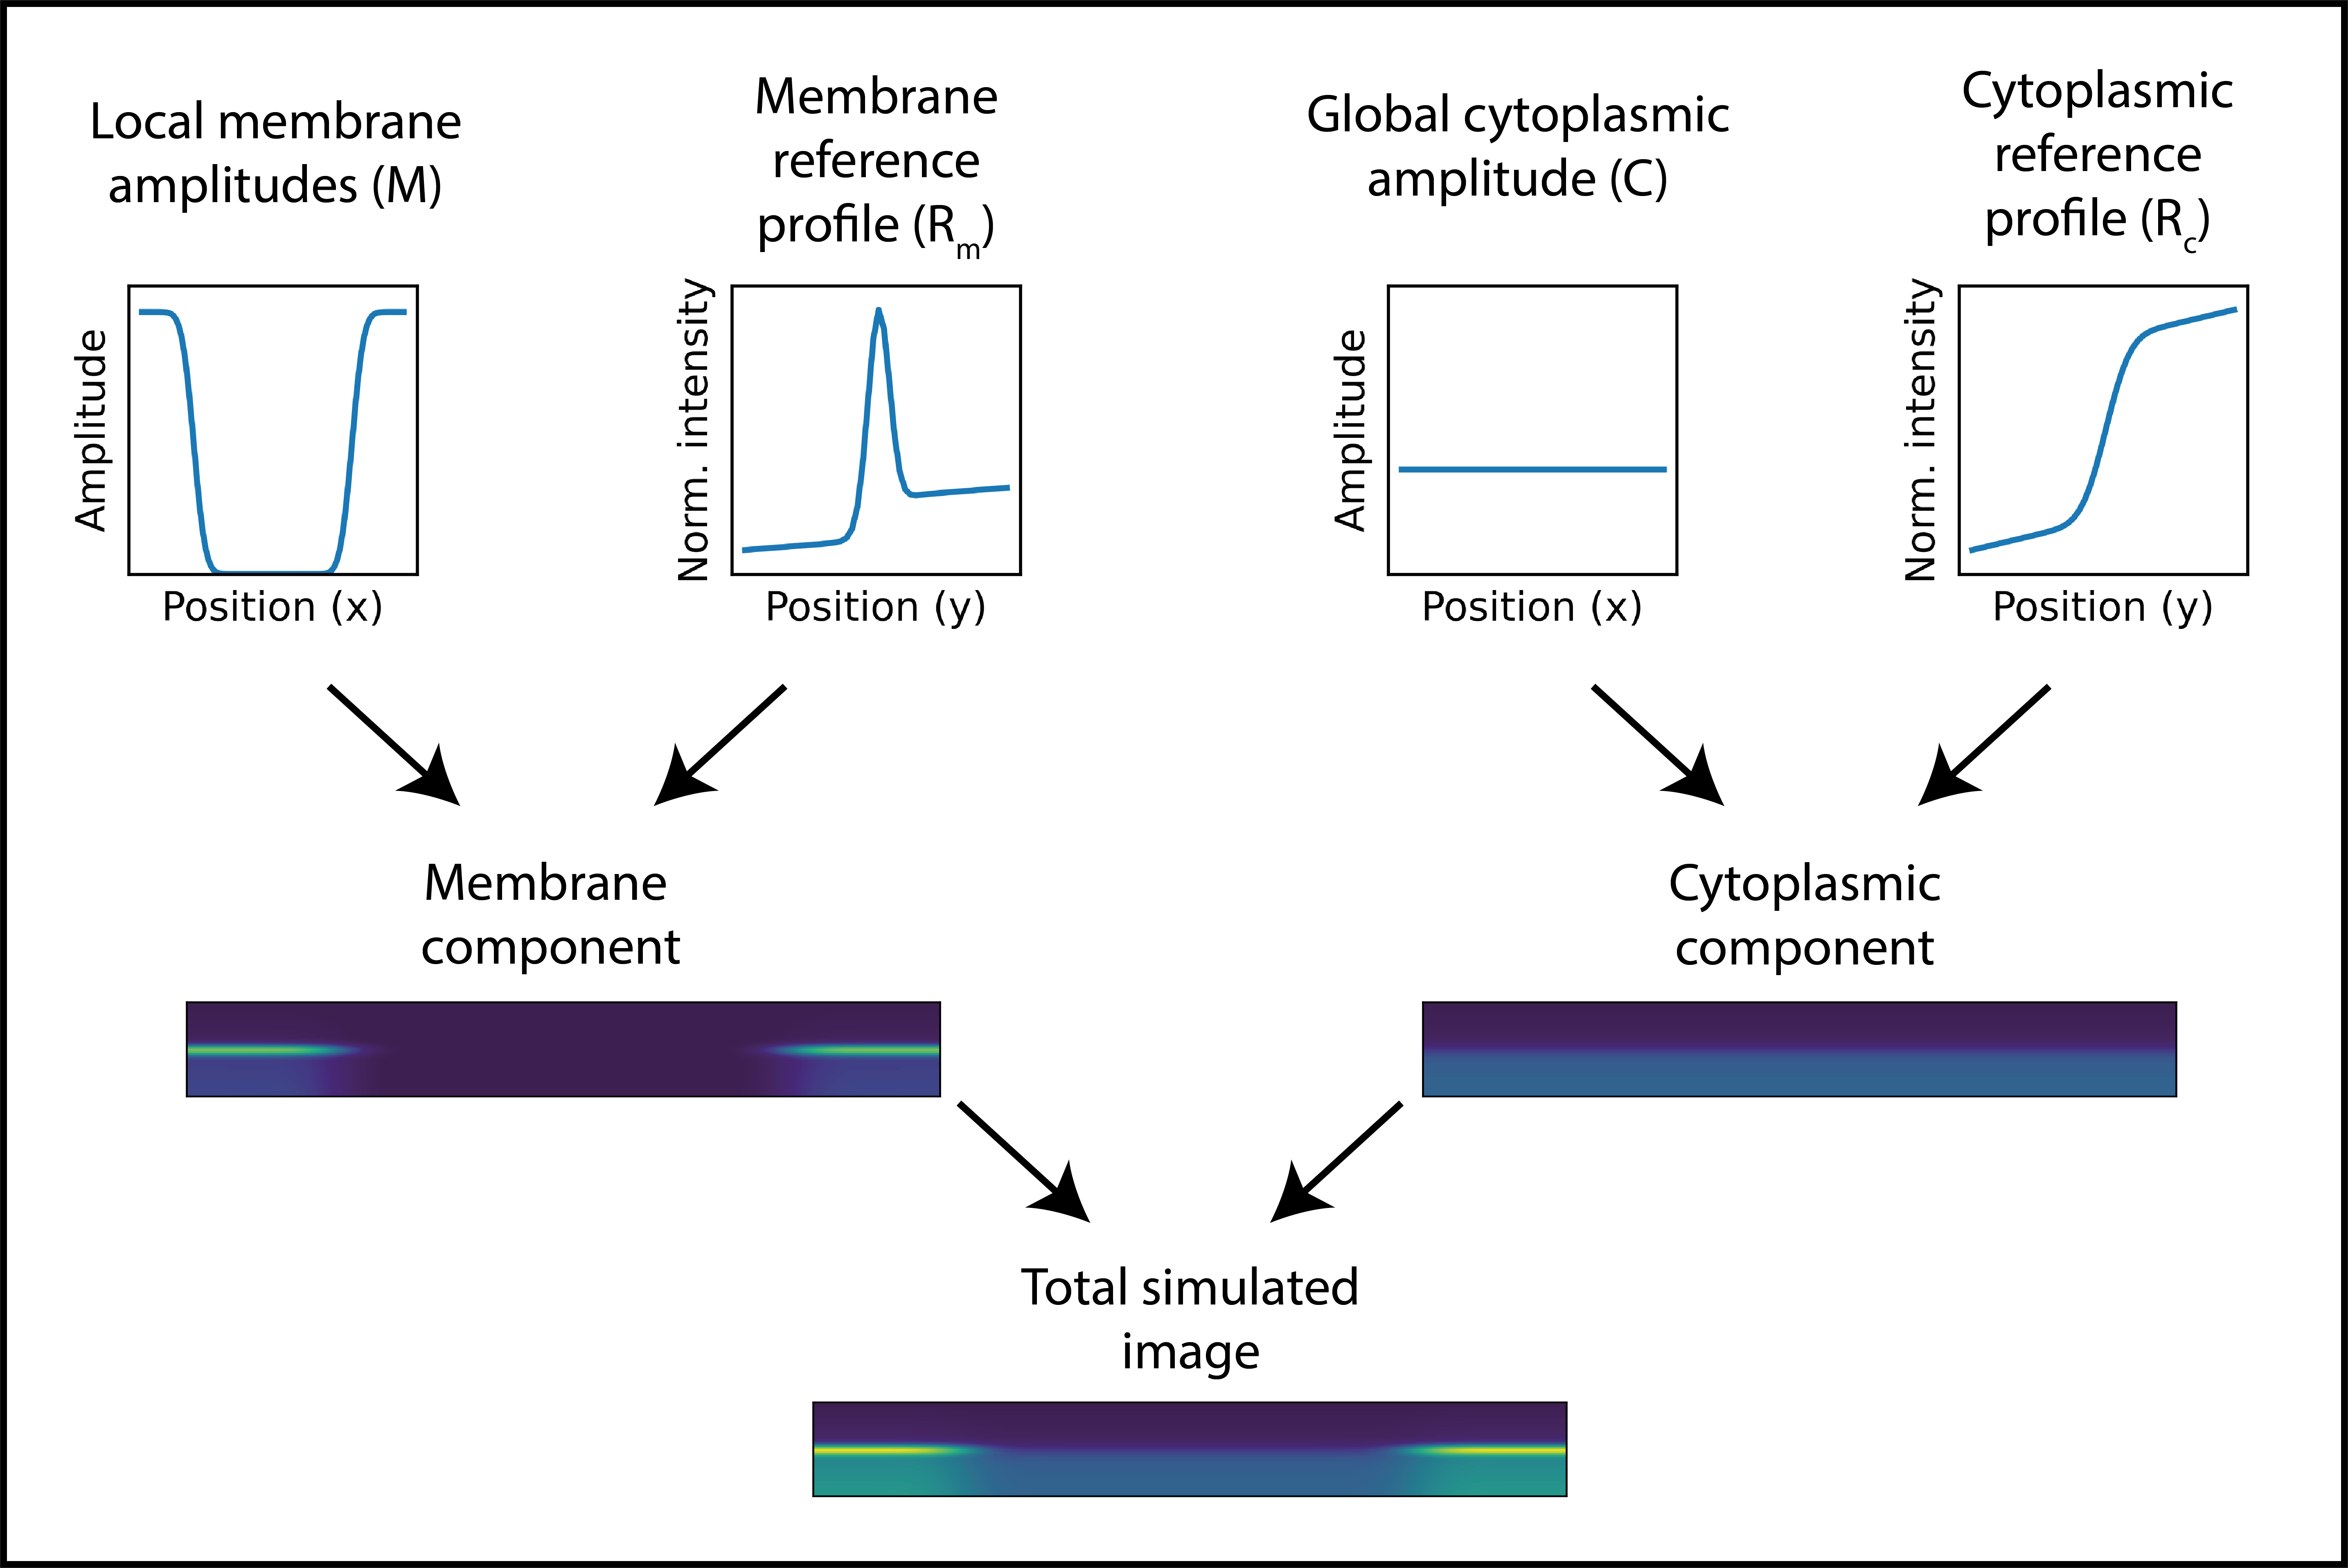
\includegraphics[scale=1.15]{memquant_model_schematic}
\centering
\mycaption{A model for simulating membrane and cytoplasmic fluorescence signal at the cortex}{
Simulated images of straightened cortices are described as the sum of membrane and cytoplasmic signal components. The membrane component is described as a 1D array of amplitudes ($M$), representing concentrations around the circumference of the embryo, convolved with a membrane reference profile ($R_m$). The cytoplasmic component is described as a single uniform amplitude ($C$) convolved with a cytoplasmic reference profile ($R_c$). Blur/scatter in the x dimension is ignored as adjacent positions are assumed to be similar.
}
\label{fig:memquant_model_schematic}
\end{figure}

$R_c$ can easily be predefined by imaging embryos in which all protein is cytoplasmic (\cref{fig:memquant_cyt_profile}). If we assume for now that $R_m$ is also predefined, then $M$ and $C$ for a given embryo can be determined by fitting a straightened image to the model presented in \cref{fig:memquant_model_schematic}. (At this point concentrations will be in arbitrary units, but I'll return to this point later). Whilst $R_m$ is in fact not predefined, given the constraints imposed by cytoplasmic uniformity, only a model with an appropriate $R_m$ will be able to create simulated images that closely match experimental images. (Imagine, for example a model with a Gaussian membrane reference profile, which would clearly fail to capture graded interior signal). Therefore, under conditions such as these, in which we have a uniform cytoplasmic component and a graded membrane component, $R_m$ need not be predefined, and can simply be fit to the data along with the concentration parameters. To perform this kind of optimisation, I have developed a gradient descent approach based on differentiable programming, which I describe below.\\


\subsection{A gradient descent protocol for image quantification}

Gradient descent is a popular optimisation strategy used for a number of machine learning applications. When optimising a model described by a series of parameters, the idea of gradient descent is to calculate the partial derivative of each parameter with respect to a loss term (e.g. mean squared error). A negative gradient for a certain parameter would imply that an increase in that parameter would decrease the loss term, whereas a positive gradient would imply the opposite. Therefore, to reduce loss, each input parameter can be adjusted in proportion to the negative of its partial derivative. Starting with a set of initial conditions, this procedure is iteratively repeated, adjusting parameters and calculating new gradients at each step, until the loss term reaches a minimum. \\

The utility of these methods has been greatly advanced in recent years by the development of differentiable programming tools. Commonly used for deep learning, although generalisable to other problems, these tools greatly speed up computation for complex optimisation procedures by automatically calculating gradients, rather than relying on numerical methods, using a process known as backpropagation. In addition, extensions to the basic gradient descent algorithm have proven effective at speeding up convergence and preventing entrapment in local minima \citep{Sun2019}. \\

In the case of this particular problem, the procedure is described in \cref{fig:memquant_forward_and_back_propagation}. Given a set of parameters ($M$, $C$, $R_m$, $R_c$), a forward propagation step simulates an image, and this is compared to the ground truth image to calculate a loss term. Backpropagation then calculates the gradient of each of the input parameters with respect to this loss term. At this point, we can adjust some or all of the input parameters according to these gradients. Repeating this cycle of forward and back propagation will then lead to a gradual optimisation of these parameters, until the loss function reaches a minimum. \\

\begin{figure}
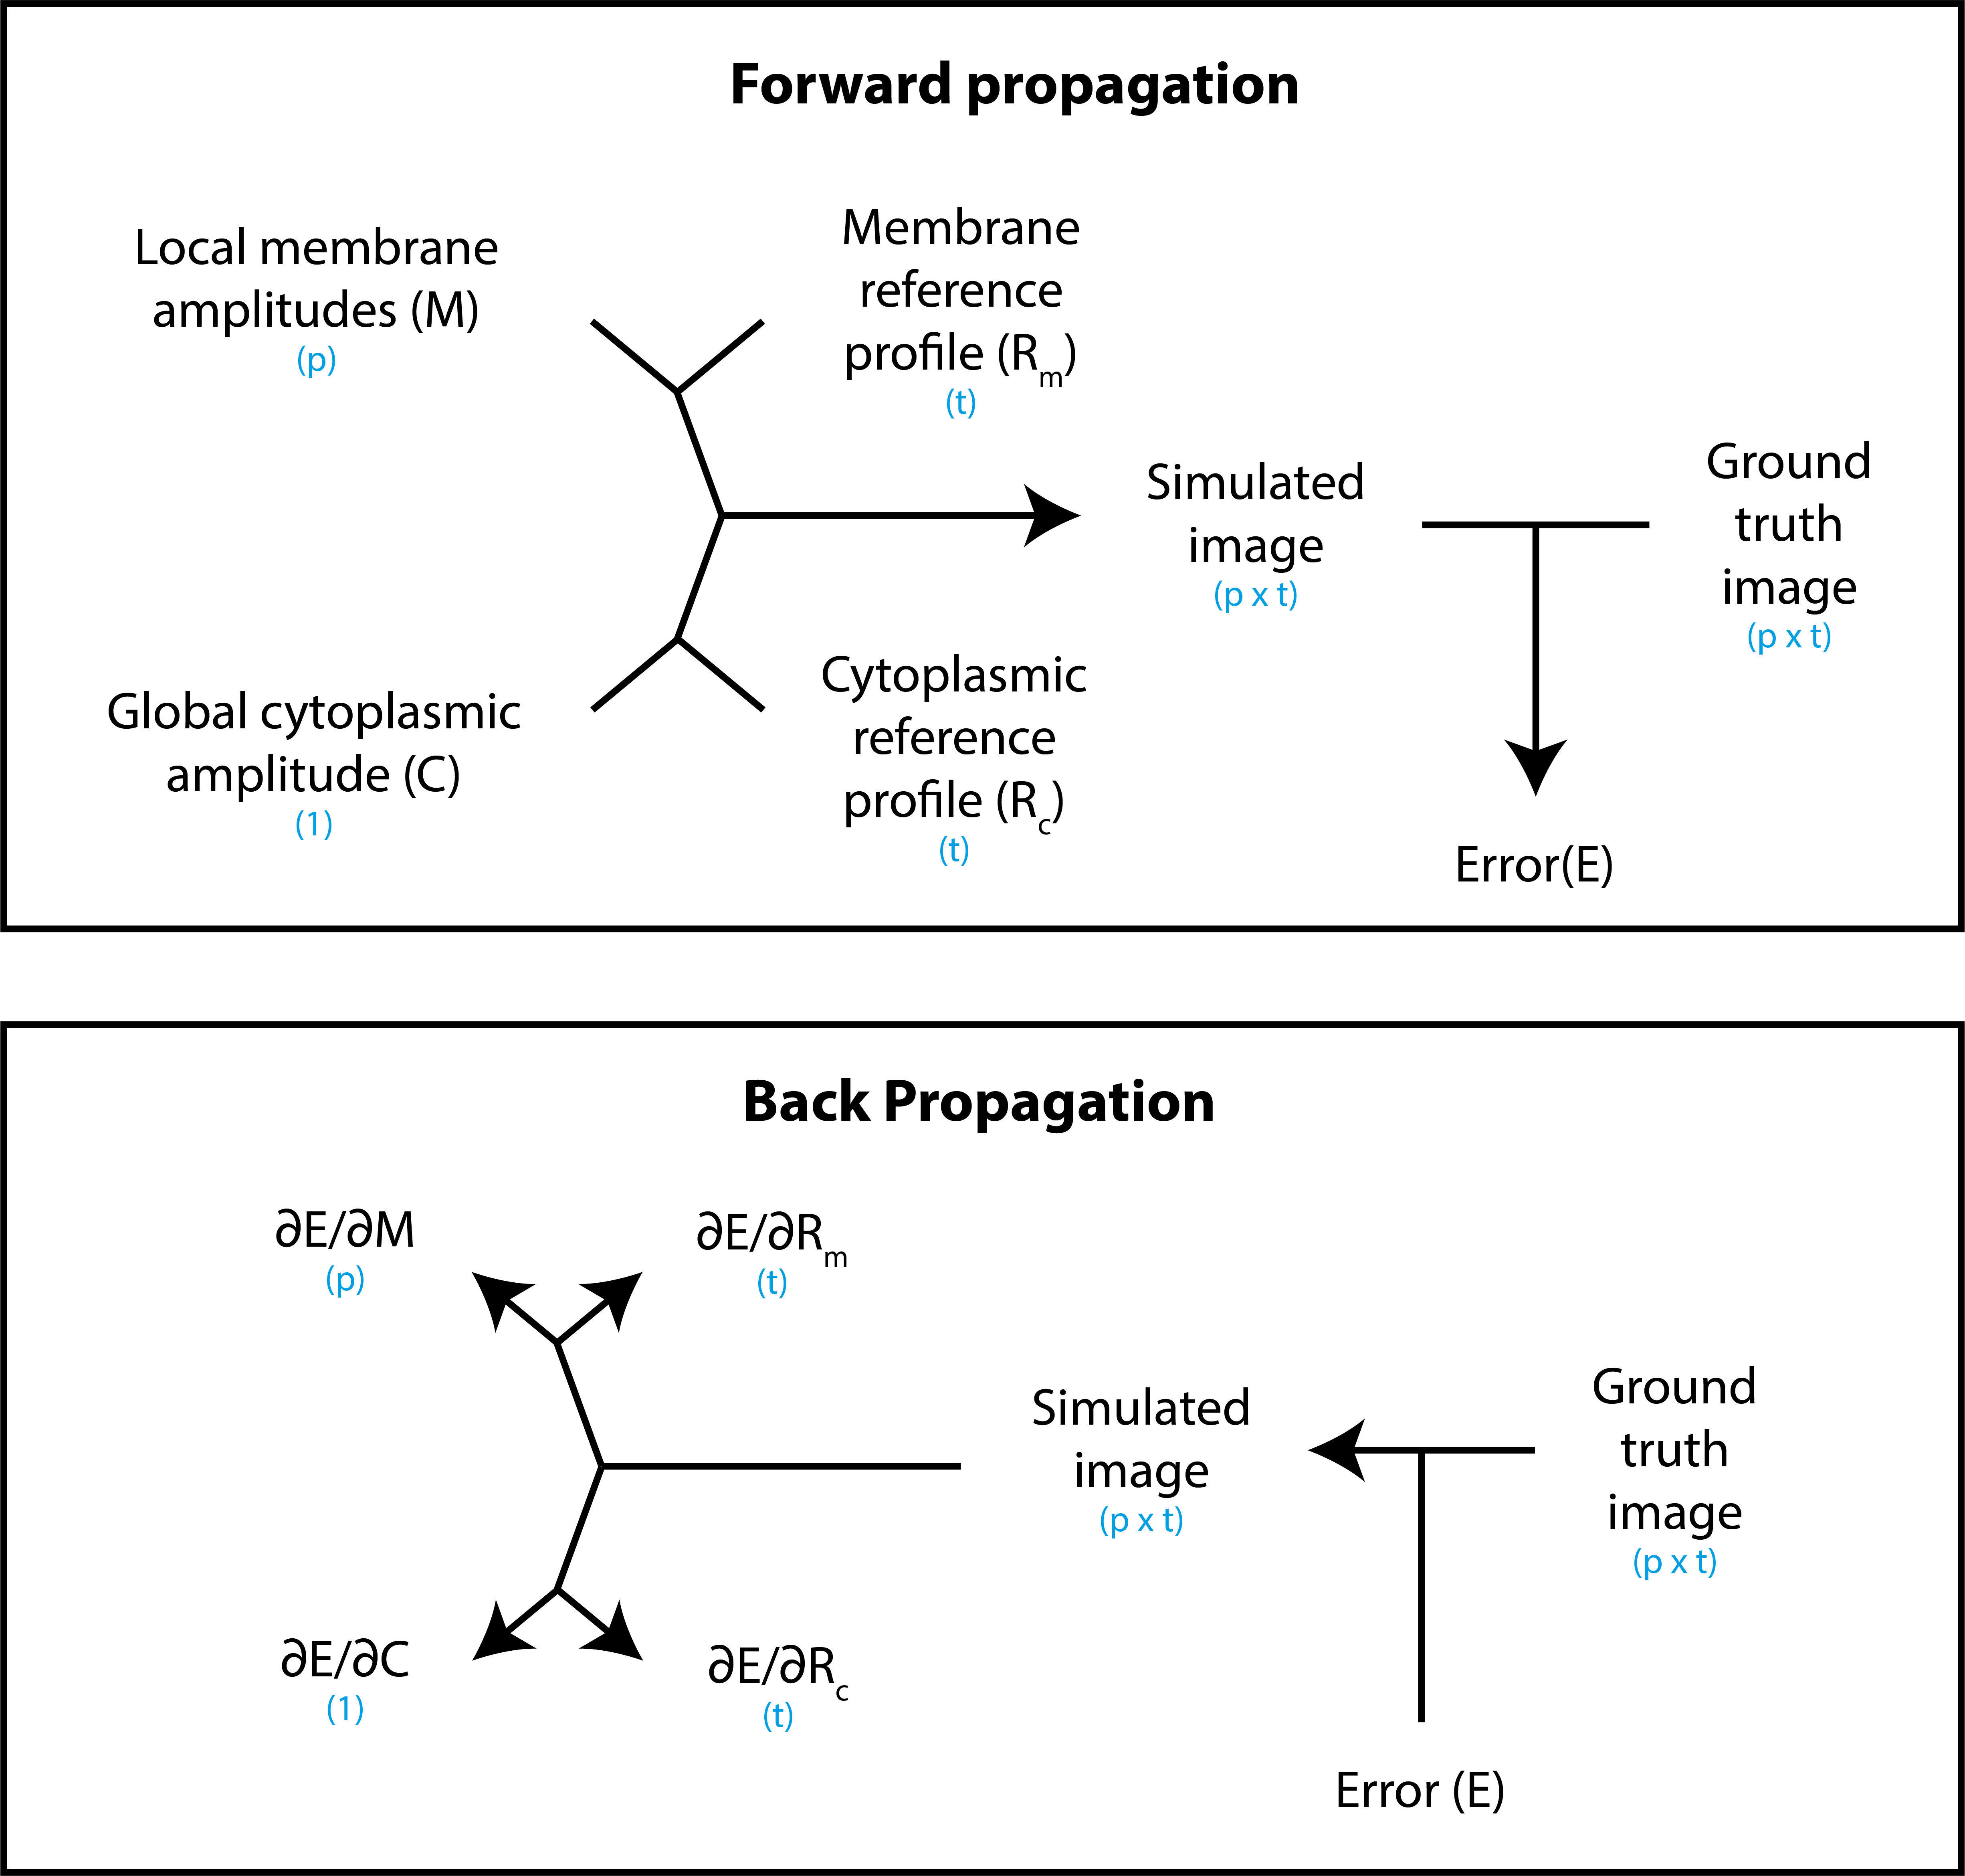
\includegraphics[scale=1.1]{memquant_forward_and_back_propagation}
\centering
\mycaption{Backpropagation gradient descent protocol for parameter optimisation}{Parameters are optimised by an iterative cycle of forward and back propagation. In the forward propagation step (top), an image is simulated given input parameters $M$, $C$, $R_m$, $R_c$, and compared to the ground truth image to calculate a loss term. In the back propagation step (bottom) gradients of the loss term with respect to each of the input parameters are calculated using the chain rule method. A subset of the input parameters can then be changed according to these gradients, which will depend on the procedure (e.g. \cref{fig:memquant_membg_training} vs \cref{fig:memquant_benchmarking_ph_rundown}). This process is repeated many times until optimisation reaches a plateau. Dimensions of the variables are shown in blue, where p represents the number of positions to fit around the cortex, and t represents the thickness of the straightened image.}
\label{fig:memquant_forward_and_back_propagation}
\end{figure}

To test this approach, I built a model using the differentiable programming package Tensorflow \citep{Abadi2016}, and first applied it to images of polarised PAR-2. The model was initiated with all concentrations ($M$ and $C$) equal to zero, and $R_m$ initiated as a Gaussian. For $R_c$ I used a measured profile (\cref{fig:memquant_cyt_profile}), and this was not adjusted during training (\cref{fig:memquant_membg_training}A). Using an Adam optimiser \citep{Kingma2015} with a learning rate of 0.01, all other parameters ($M$, $C$ and $R_m$) were then adjusted iteratively until a plateau was reached (250 steps), as shown in \cref{fig:memquant_membg_training}B. The final simulated image, composed of a uniform cytoplasmic component and a nonuniform membrane component, closely matches the ground truth image (\cref{fig:memquant_membg_training}C).\\


\begin{figure}
\includegraphics[scale=1]{memquant_membg_training}
\centering
\mycaption{Separation of membrane and cytoplasmic signal in an image of mNG::PAR-2}{
\textbf{(A)} Schematic demonstrating the optimisation procedure, highlighting the input parameters to be optimised in red.
\textbf{(B)} $R_m$, $M$ and $C$ throughout the training procedure for an mNG::PAR-2 expressing polarised embryo. $R_m$ was initiated as a Gaussian (radius = x) centred at zero, $M$ and $C$ initiated as zero.
\textbf{(C)} Final simulated image compared to the ground truth image. Right panel shows profiles at specified positions (solid = ground truth, dashed = simulated). Uniform cytoplasmic component shared between profiles indicated in gray.
}
\label{fig:memquant_membg_training}
\end{figure}

% more here on reproducibility.

\subsection{Segmentation}

In addition to the parameters already mentioned, the full model also includes a series of alignment parameters, which can also be trained by gradient descent, allowing the model to freely align to the data in the y direction. As a result, ground truth images do not need to be accurately segmented prior to optimisation, and rough manual ROIs are fine to use. This is particularly useful for timelapse movies, where, even if the embryo undergoes shape changes, only a single manual ROI needs to be provided. An additional outcome of alignment is that the offset parameters can be used to refine the original ROI, meaning that the method can serve as a tool for computational segmentation. Refined ROIs can then be used to re-straighten the cortex, and optimisation repeated (\cref{fig:memquant_segmentation}). Overall, this allows cortices to be segmented with subpixel accuracy with minimal manual input. In theory, the initial manual step could also be automated using deep learning methods to create a fully automated pipeline \citep{Minaee2021}.\\

\begin{figure}
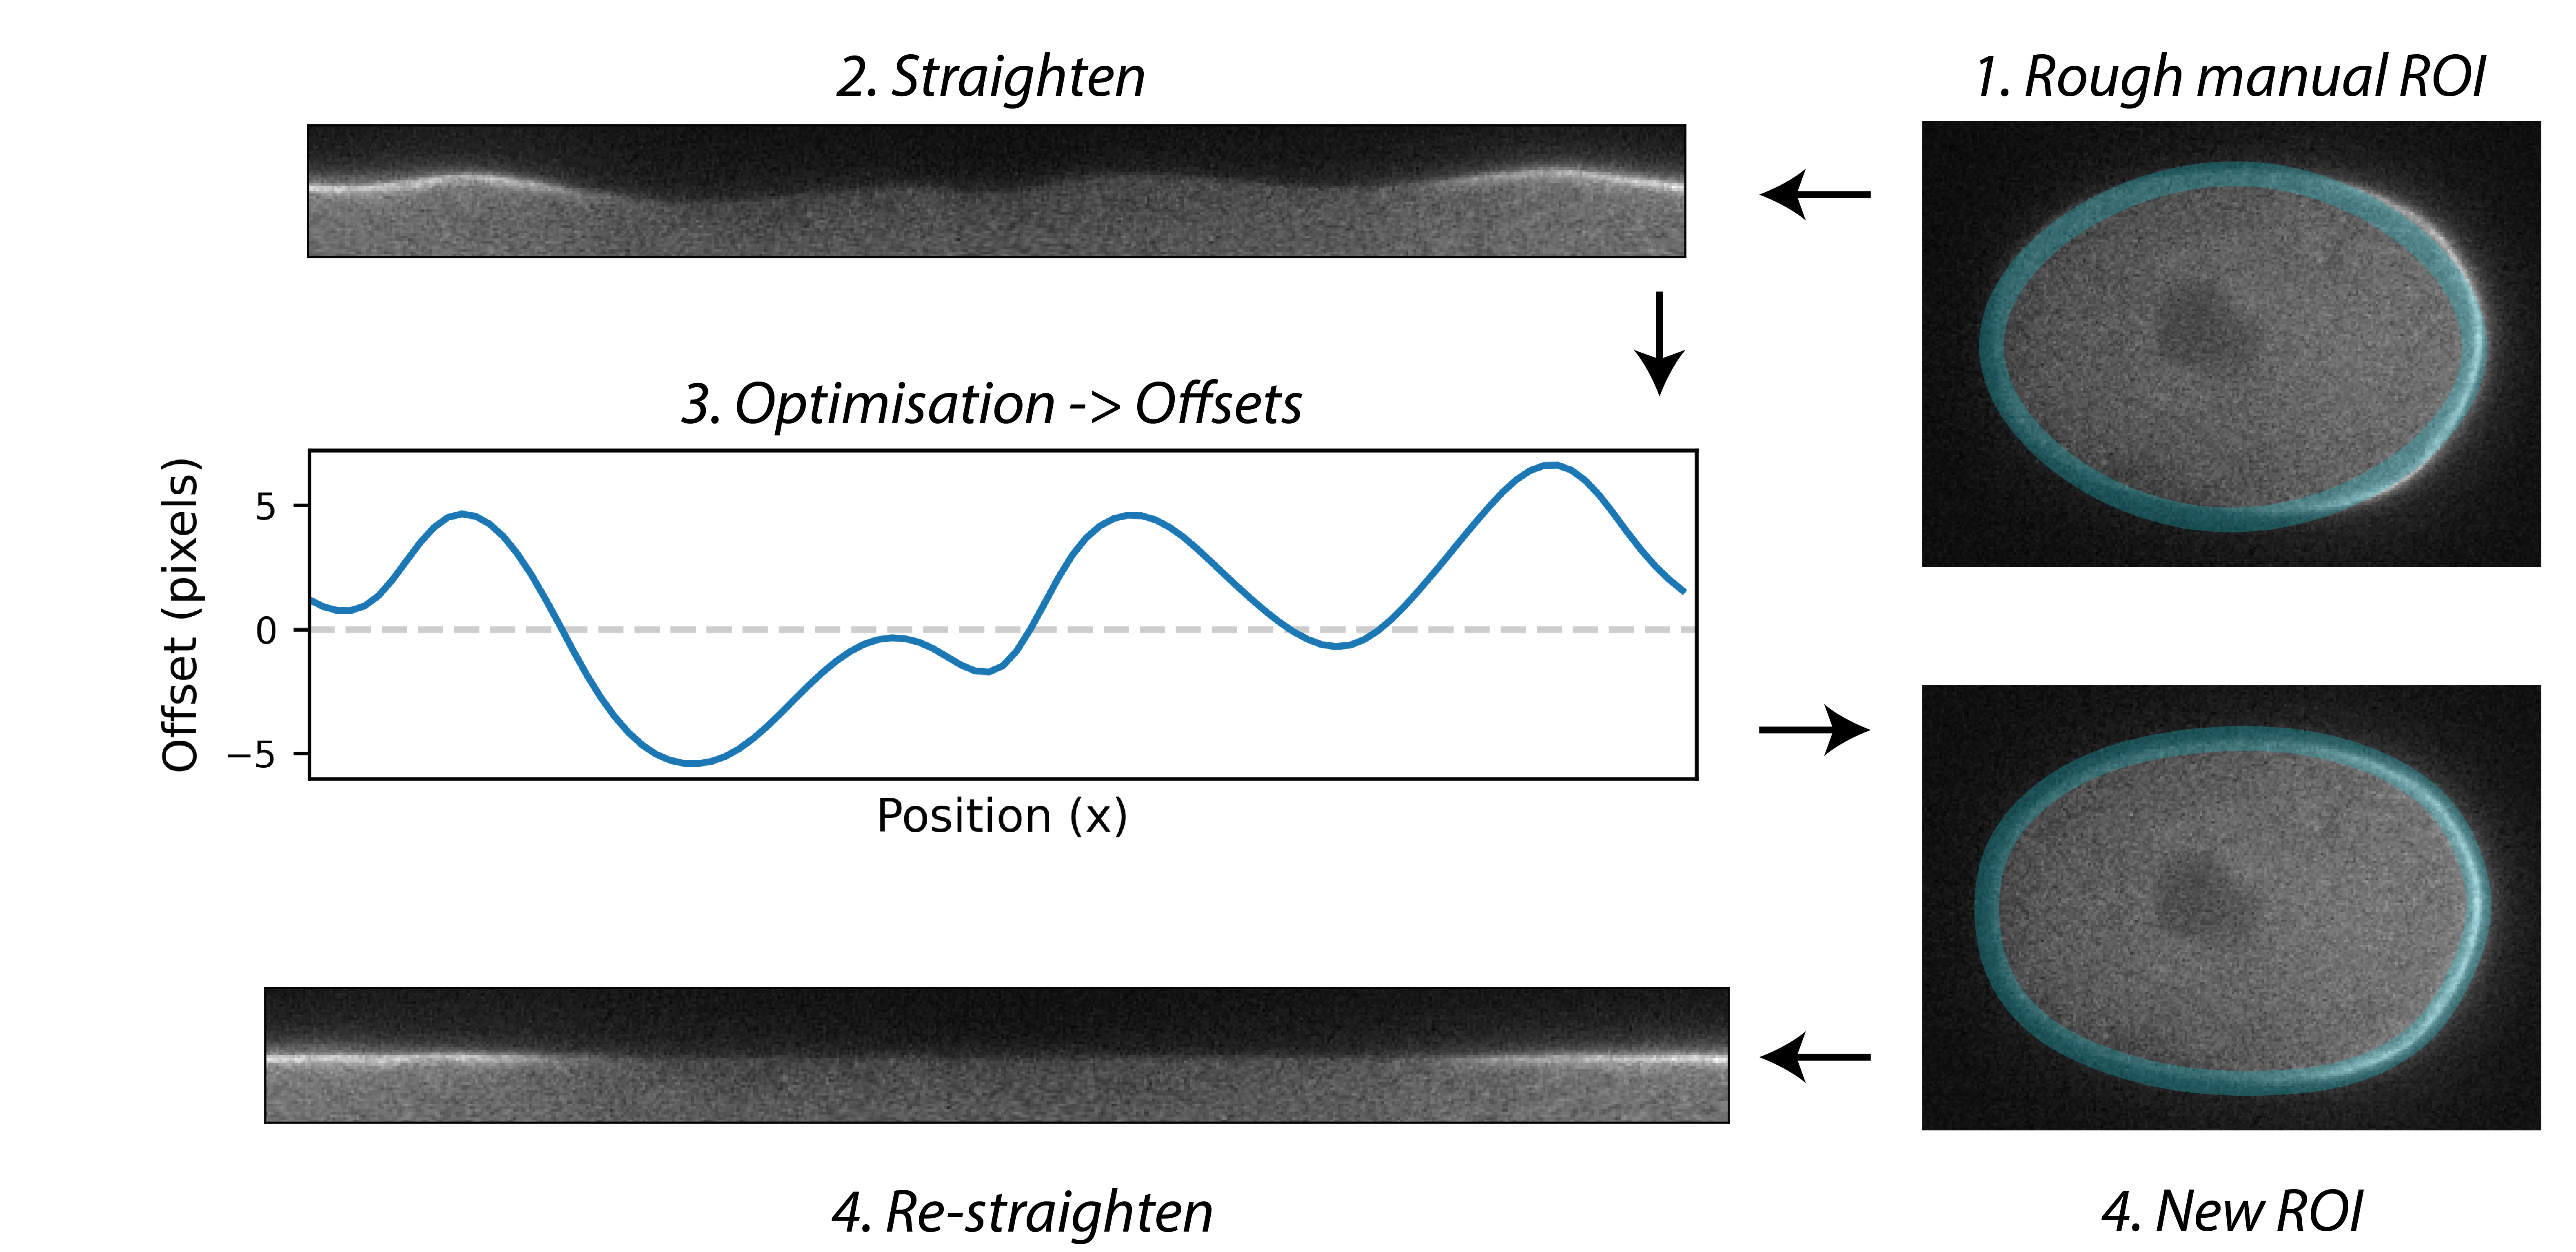
\includegraphics[scale=1]{memquant_segmentation}
\centering
\mycaption{Semi-automated segmentation algorithm}{
Segmentation is initiated with a rough manual ROI. The cortex is then straightened and fit to the model yielding, among other parameters, parameters describing offset at each position along the x dimension. These offsets can then be used to adjust the initial ROI, and re-straighten the cortex. The re-straightened cortex can then be refit to the model to give concentration parameters. Shown here for an embryo expressing mNG::PAR-2(L109R).
}
\label{fig:memquant_segmentation}
\end{figure}


\subsection{Benchmarking the method}

The method described so far is limited to cases of images with polarised membranes. However, as discussed previously, $R_m$, which is a function of local geometry and optical properties, should be a constant function applicable to all embryos. Therefore, much like I used a predefined $R_c$ when fitting images of polarised PAR-2, images of proteins without a polarised membrane can be quantified by using an $R_m$ derived from a calibration procedure on polarised images. \\

To test this method, I performed quantification on images of embryos expressing the uniform plasma membrane probe GFP::PH with variable expression levels (\cref{fig:memquant_benchmarking_ph_rundown}B), obtained by performing an RNAi rundown using XFP RNAi feeding bacteria (see Methods). In this case, I used a predefined $R_m$ and $R_c$, and only optimised $M$ and $C$ (as well as the alignment parameters described in the previous section) (\cref{fig:memquant_benchmarking_ph_rundown}A). Images were initiated with a rough manual ROI and segmented using the method described in \cref{fig:memquant_segmentation} prior to final quantification. Compatible with expected linear membrane binding kinetics, we can see that the method gives a tight linear relationship between cytoplasmic and membrane concentrations (\cref{fig:memquant_benchmarking_ph_rundown}C). N2s are also accurately described as having cytoplasmic and membrane concentrations close to zero.\\

\begin{figure}
\includegraphics[scale=1]{memquant_benchmarking_ph_rundown}
\centering
\mycaption{Quantification of GFP::PH expressing embryos reveals a linear relationship between membrane and cytoplasmic concentrations}{
\textbf{(A)} Schematic demonstrating the optimisation procedure, highlighting the input parameters to be optimised in red.
\textbf{(B)} Images of GFP::PH expressing embryos with varying dosages of GFP::PH, obtained by RNAi rundown.
\textbf{(C)} Membrane vs. cytoplasmic concentrations for the full dataset of embryos. Empty circles represent untagged N2 embryos. Embryos in (B) represented by blue, orange and green circles.
\textbf{(D)} Cross-cortex profiles averaged over the entire circumference of the embryo vs. GFP::PH dosage. Colour coding as in (C).
}
\label{fig:memquant_benchmarking_ph_rundown}
\end{figure}

I next investigated how robust the pipeline is to changing signal-to-noise ratios, using images of three GFP::PH embryos with varying expression levels and adding varying levels of Gaussian pixel noise (\cref{fig:memquant_benchmarking_noise}A). As seen in \cref{fig:memquant_benchmarking_noise}B and C, pixel noise adds noise to the resulting quantifications, but doesn't bias the data in any direction. Quantification of untagged N2s is also not biased by noise (\cref{fig:memquant_benchmarking_noise}B/C grey points).\\

\begin{figure}
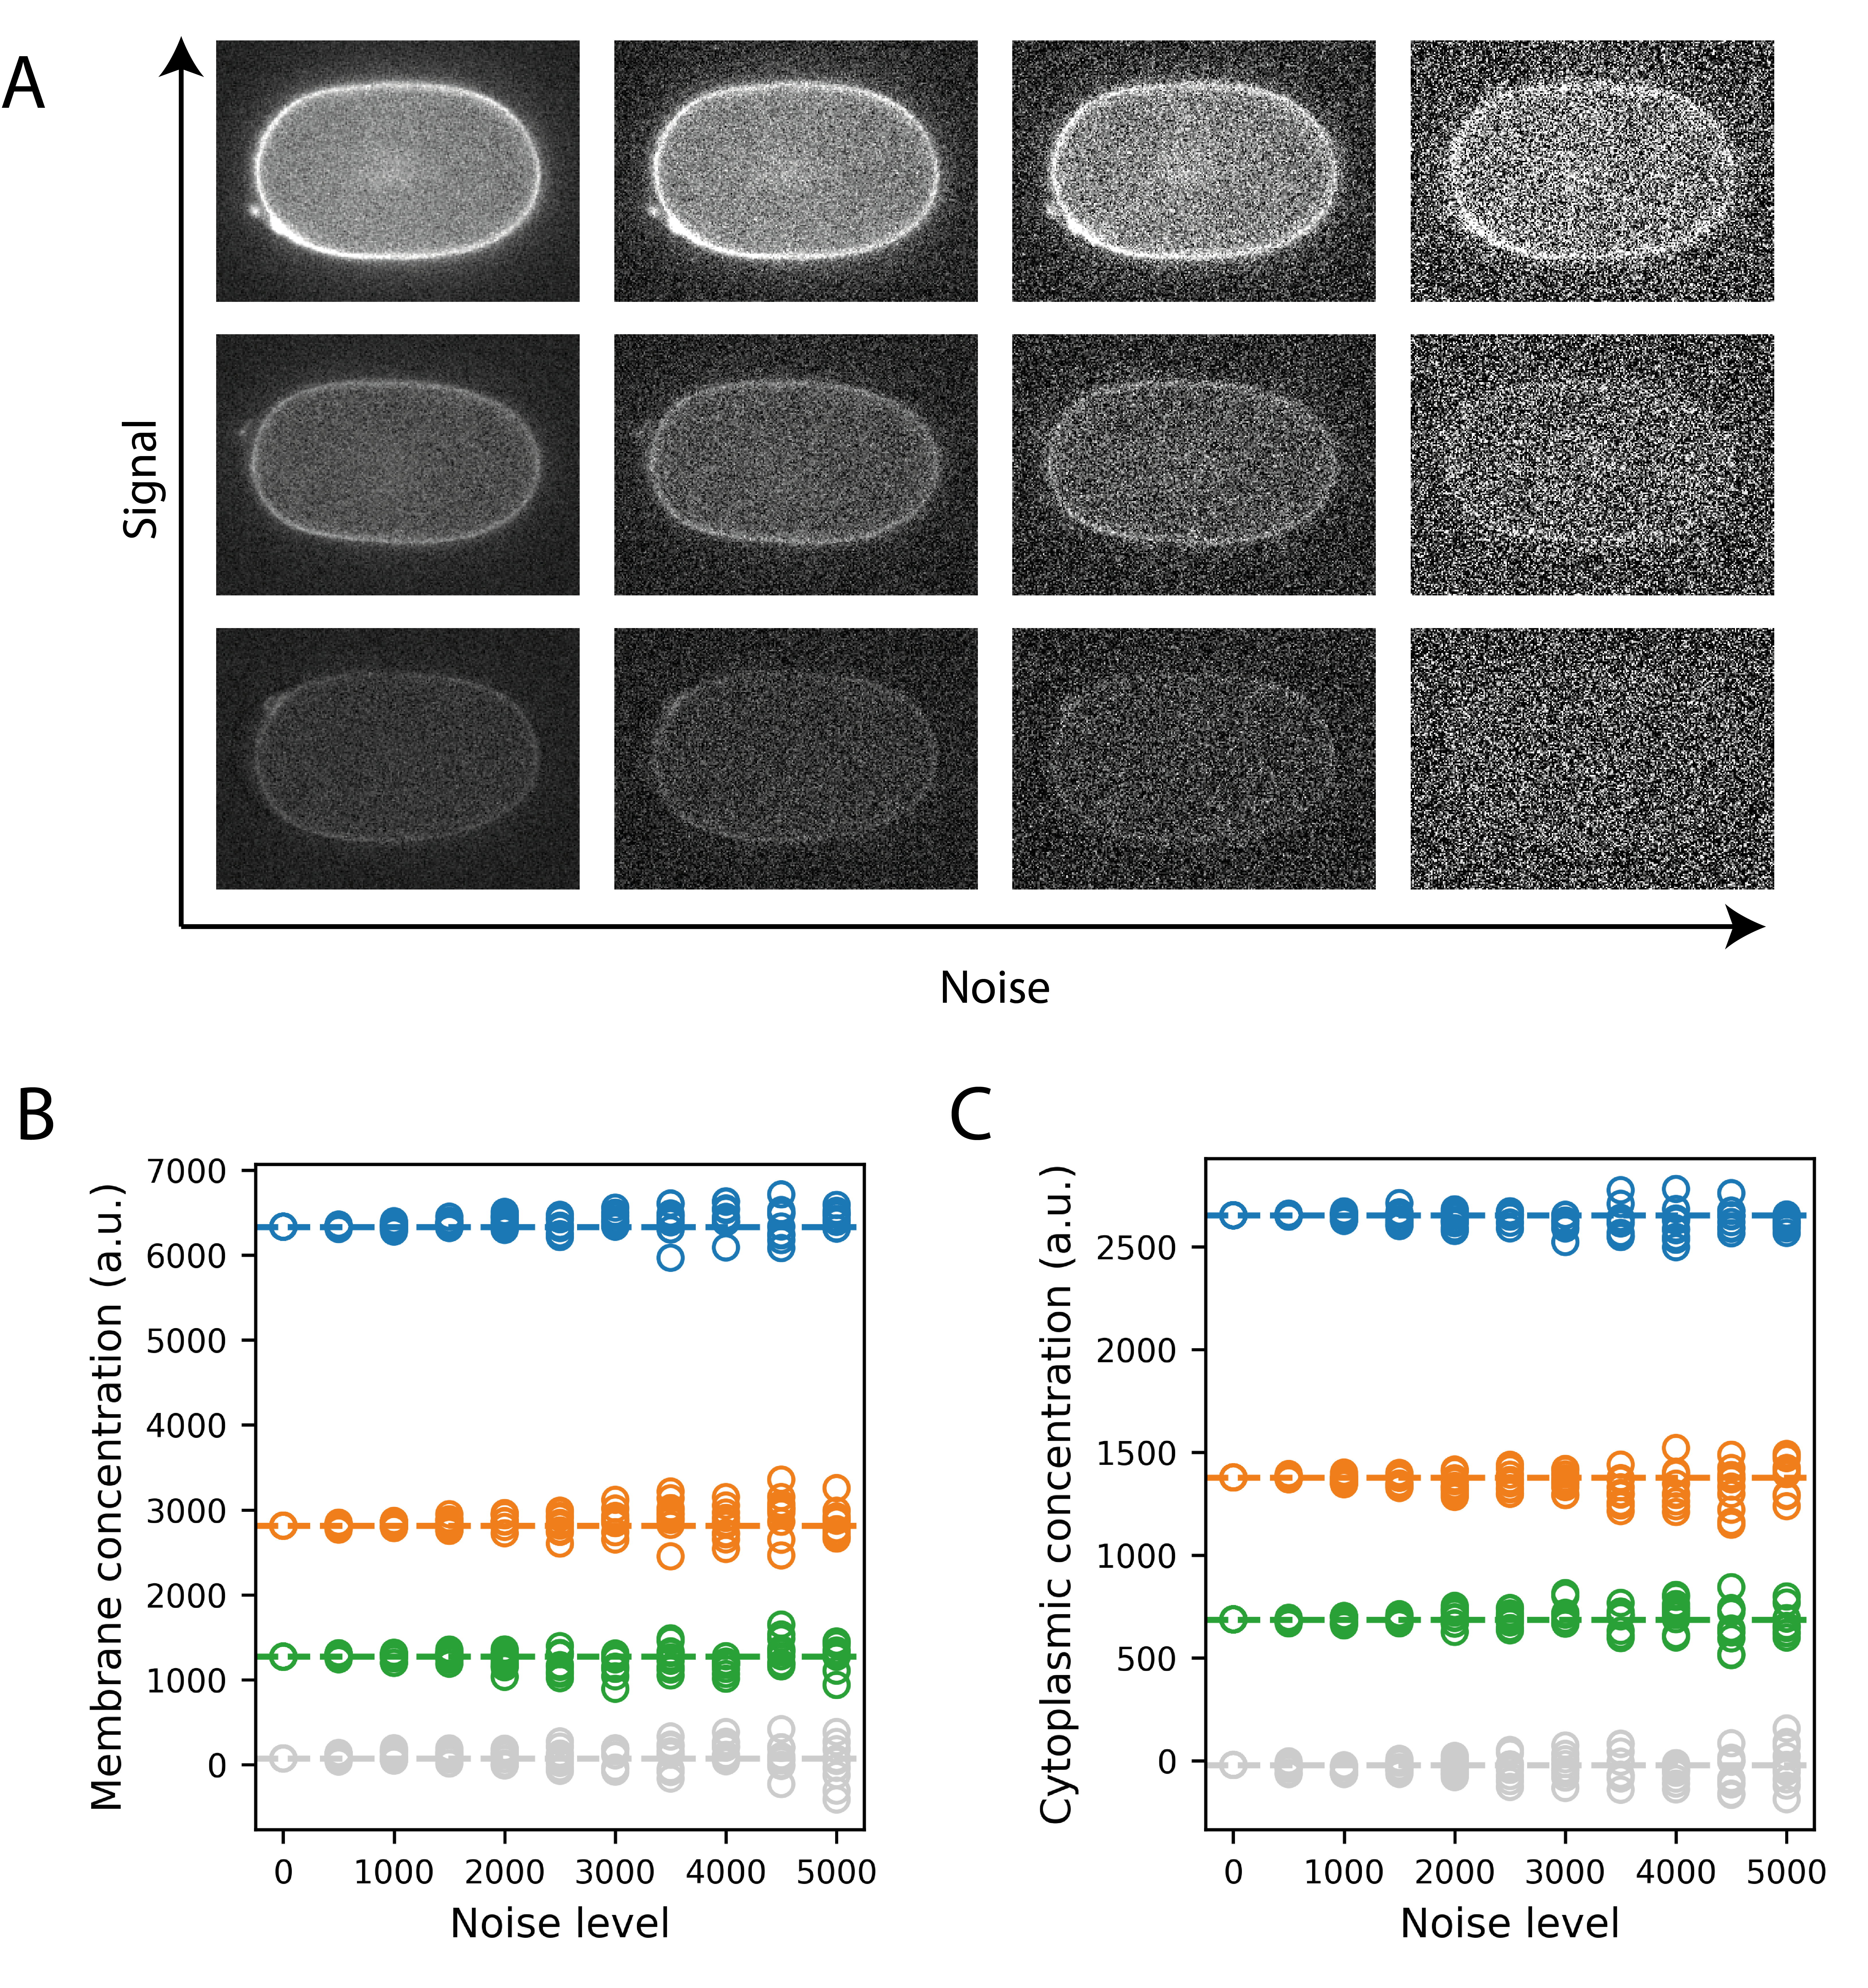
\includegraphics[scale=0.95]{memquant_benchmarking_noise}
\centering
\mycaption{Quantifications of membrane and cytoplasmic concentrations are robust to pixel-noise}{
\textbf{(A)} Images of three GFP::PH expressing embryos with varying amounts of GFP::PH subject to varying levels of Gaussian pixel noise.
\textbf{(B)} Quantifications of membrane concentration (averaged over the entire embryo) for the three embryos in (A) subject to varying levels of pixel noise, colour coded by embryo. For each noise level 10 images were generated for each embryo, and each images was quantified and plot as a single point. Similar analysis for an untagged N2 embryo is also shown (gray). Dashed lines indicate quantification at noise=0.
\textbf{(C)} Quantifications of cytoplasmic concentration for the three embryos in (A) and a single N2 embryo subject to varying levels of pixel noise. Procedure as in (B). Noise level defined as standard deviation of Gaussian noise added to the image. 
}
\label{fig:memquant_benchmarking_noise}
\end{figure}


\subsection{Calibrating concentration units}

As $M$ and $C$ are in arbitrary units (effectively in units of their own respective reference profiles), a conversion parameter, is required to put them into common units. To calibrate this conversion parameter, I quantified the effects on $M$ and $C$ measurements of redistributing a fixed pool of protein from the cytoplasm to the membrane. To do this, I used an optogenetics system with a plasma membrane bound PH::eGFP::LOV to move a cytoplasmic pool of ePDZ::mCherry to the membrane (Fielmich et al., 2018). Embryos were exposed to blue light for 10 seconds, which promotes binding between ePDZ and LOV, leading to a rapid uniform recruitment of ePDZ::mCherry to the membrane and a reduction in the concentration in the cytoplasm (\cref{fig:memquant_optogenetics}). Where ePDZ::mcherry is expressed alone, this localisation shift isn't observed (\cref{fig:memquant_optogenetics}, grey points).\\

\begin{figure}
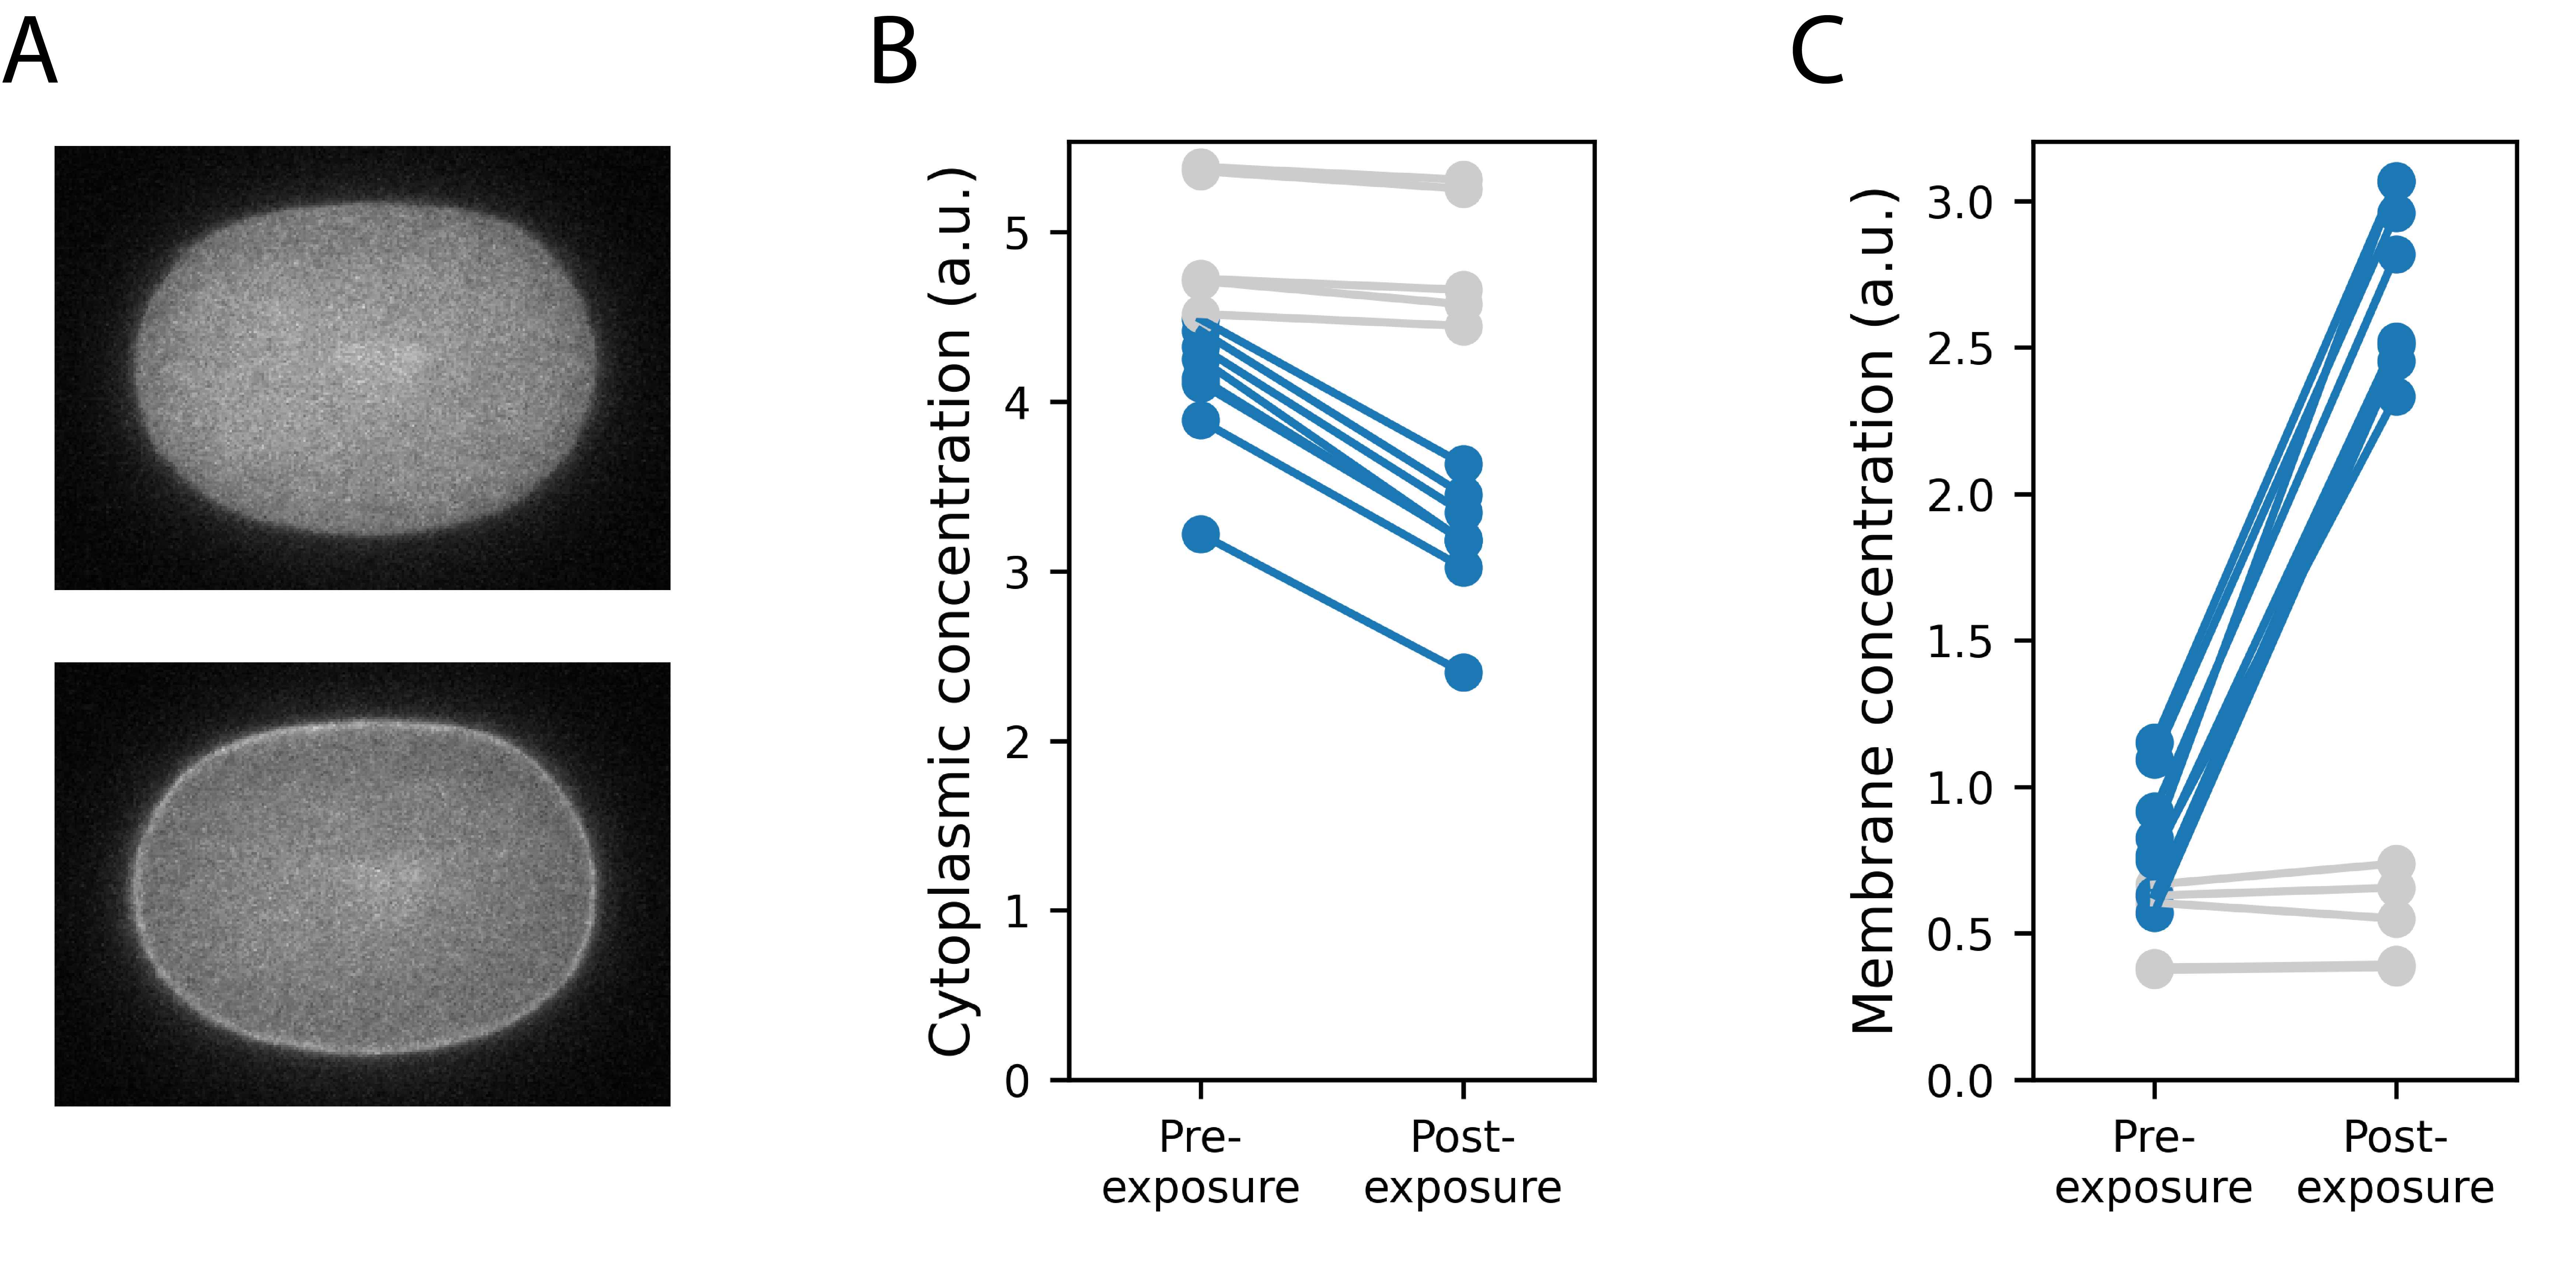
\includegraphics[scale=1]{memquant_optogenetics}
\centering
\mycaption{Redistribution of fluorescent signal from cytoplasm to membrane using optogenetics}{
\textbf{(A)} ePDZ::mCherry before (top) and after (bottom) exposure to blue light, in an embryo also expressing PH::eGFP::LOV.
\textbf{(B)} Cytoplasmic concentration of ePDZ::mCherry (in arbitrary units) before and after blue light exposure for embryos with (blue) and without (gray) PH::eGFP::LOV. 
\textbf{(C)} Membrane concentration of ePDZ::mCherry (in arbitrary units) before and after blue light exposure for embryos with (blue) and without (gray) PH::eGFP::LOV. 
}
\label{fig:memquant_optogenetics}
\end{figure}

Whilst there is significant protein relocalisation in the optogenetic system, the total amount of protein before and after blue light exposure can be assumed to be constant. This total amount, $T$, can be expressed as the $C$ value that would be expected if all tagged molecules were in the cytoplasm, given by equation \ref{eq:t} where $\psi$ is the surface-area to volume ratio of the cell ($= 0.174 \mu m ^ {-1}$ \citep{Goehring2011a}). Given that $M$ is in different arbitrary units to $C$, a conversion parameter, $c$, is required:

\begin{equation}
T = C + \psi c M
\label{eq:t}
\end{equation}

Given that $T$ is the same before and after exposure, $c$ can be calculated, on an embryo by embryo basis, by comparing the gain in $M$ post-exposure to the loss in $C$:

\begin{equation}
c = \frac{C_{pre \textrm{-} exposure} - C_{post  \textrm{-} exposure}}{\psi (M_{post  \textrm{-} exposure} - M_{pre  \textrm{-} exposure})}
\end{equation}\\

Performing this analysis on the dataset in \cref{fig:memquant_optogenetics} (blue points) gives a value of $c$ = 2.88 $\pm$ 0.12 $\mu$m (mean $\pm$ SD), which can be used to convert membrane concentrations to the same common units as cytoplasmic concentrations (i.e. $\mu m^{-3}$ for cytoplasmic concentrations and $\mu m^{-2}$ for membrane concentrations). Note that these concentrations are still arbitrary in the sense that they do not indicate absolute concentrations (i.e. absolute number of molecules per unit area). However, for much of the analysis in the following sections, where the aim is to measure membrane affinities (membrane to cytoplasmic ratios) this will not be an issue, although I'll return to this point in section x.\\

\clearpage
\subsection{Discussion}

Accurate quantification of features from images relies on the ability to separate overlapping signals and correctly attribute signals to their source. In this section, I have described a two-step pipeline designed for accurate quantification of cytoplasmic and membrane concentrations from midplane images of \textit{C. elegans} zygotes. The first step involves separation of autofluorescence and fluorophore signal, and the second step involves separation of signals from cytoplasmic and membrane protein. The overall pipeline is not specific for any particular microscope, and makes no assumptions about the spectral characteristics of the signal components or the optical properties of the imaging system/sample. Whilst the SAIBR method isn't fundamentally tied to \textit{C. elegans}, and has been shown to apply to other systems, the method for separation of cytoplasmic and membrane signals is less generalisable, and a number of assumptions in the model presented here are firmly linked to the simple and reproducible geometries of \textit{C. elegans} zygotes and PAR protein patterns. Nevertheless, the ability to confidently quantify relative membrane and cytoplasmic concentrations in vivo brings forward new experimental possibilities for studies of the \textit{C. elegans} PAR network, and will prove fundamental to much of the work presented in the following chapters of this thesis.\\


%%%%%%%%%%%%%%%%%%%%%%%%%%%%%%%%%%%%%%%%%%%%%%%%%%%%%%%%%%
\clearpage
\chapter{Uncovering a PAR-2 positive feedback circuit}

\textbf{Detailed contributions:}\\

\clearpage
\section{Introduction}

% Most of this might work better in the main introduction section, but including here now as it's necessary to introduce the chapter.

Mutual antagonism, in which aPARs and pPARs exclude each other from the membrane through phosphorylation reactions, is generally understood to be a dominant factor driving self-organisation of PAR polarity. When coupled to with sufficiently strong spatial trigger, such as an advective flow trigger, mutual antagonism alone is sufficient to give rise to stable polarity in computer models. However, a number of experimental observations have been made which cannot be accounted for by such simple models, suggesting that other feedback mechanisms may be important.\\

Of particular interest is PAR-2, a posterior PAR scaffold which recruits the kinase PAR-1. Whilst PAR-2 is dependent on exclusion by PKC-3 for polarity, several observations have been made which appear to violate predictions from mutual antagonism models, and suggest that PAR-2 plays significant roles in polarity formation which are not fully appreciated by existing computer models.\\

\subsection{The PAR-2 polarity pathway}

As previously discussed, PAR-2 is able to initiate polarity in the absence of cortical flows (`no-flow' conditions) through an interaction with microtubules. This interaction protects PAR-2 from phosphorylation by PKC-3, which leads to localised recruitment of PAR-2 to the cortex at the posterior pole. Cortical PAR-2 then recruits PAR-1 from the cytoplasm, which antagonises aPARs through phosphorylation of PAR-3. According to a simple mutual antagonism model, if a threshold concentration of pPAR is reached in the posterior, self-organisation can be initiated, resulting in the formation of a normal polarised PAR pattern (\cref{fig:no_flow_sb_model}). \\

% Add something here about Nelio's data?

\begin{figure}
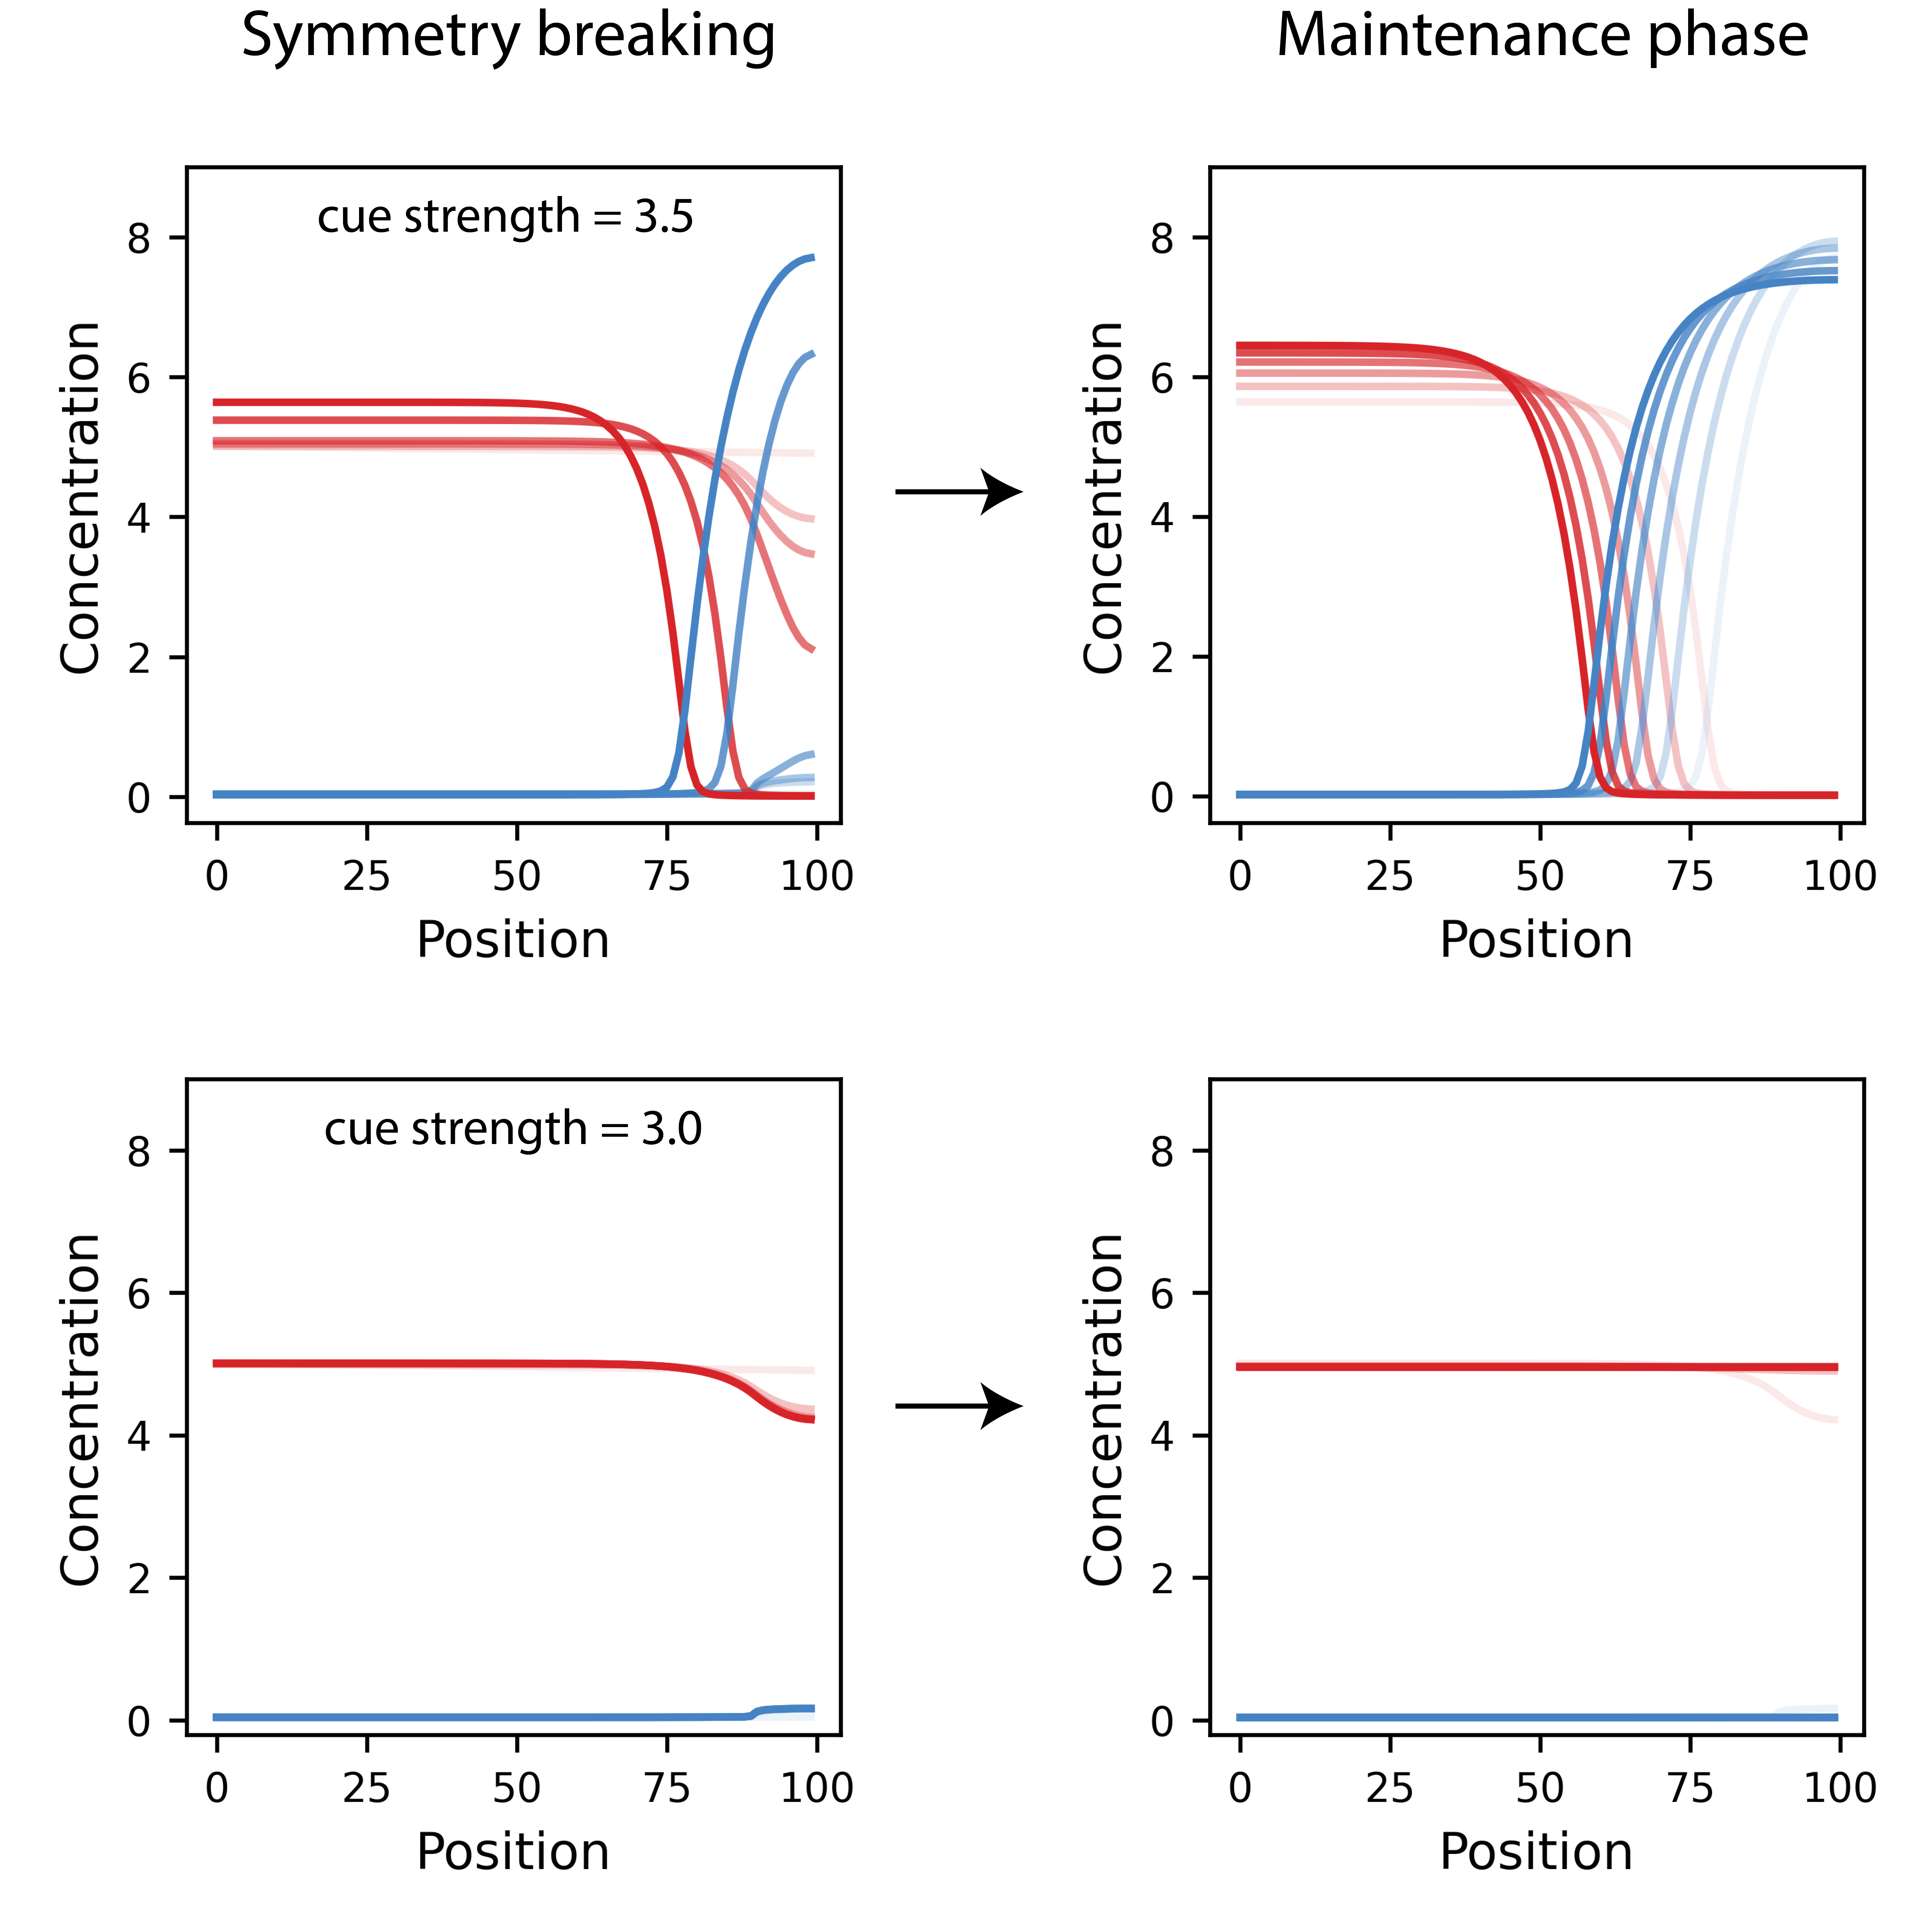
\includegraphics[scale=0.9]{no_flow_sb_model}
\centering
\mycaption{Simulating PAR polarity driven by the microtubule cue}{
Systems were simulated for 1000s with a posterior cue, modelled as a decrease in the antagonism rate from A to P in the posterior 10\% (Symmetry breaking), and then simulated for a further 1000s without a spatial cue (Maintenance phase). Cue strength represents fold change in the antagonism rate from A to P in the posterior 10\%. If the cue is sufficiently strong, a threshold pPAR concentration can be reached in the posterior to initiate self-organisation (top row).}
\label{fig:no_flow_sb_model}
\end{figure}

% Could go into a bit more detail here and show that threshold cue strength depends on off rate, as this would help explain the RING phenotype and might give more weight to the argument that the membrane affinity of the microtubule mutants may be significant

Strikingly, and in contrast to predictions from the mutual antagonism model, it has been shown that formation of a stable PAR-2 domain in these conditions does not actually require aPARs to be cleared from the posterior \citep{Motegi2011}. In \textit{par-1} mutant conditions, or with a \textit{par-3} mutant lacking the PAR-1 phosphorylation site (S950A), PAR-2 domains are able to be initiated, and spread, without corresponding clearance of aPARs, leading to spatial overlap of aPARs and pPARs in the posterior. The fact that PAR-2 can polarise without spatial information from the aPARs implies that additional positive feedback mechanisms must exist that contribute to PAR-2 polarity (\cref{fig:polarity_regimes_schematics}). Specifically, the fact that PAR-2 domains can overlap with PKC-3 implies that feedback mechanisms must exists that allow cortically enriched PAR-2 to resist or counteract antagonism from PKC-3 in the posterior. Whilst we do not have a complete picture of these feedback pathways, some insights from previous studies shed light on potential mechanisms.\\

\begin{figure}
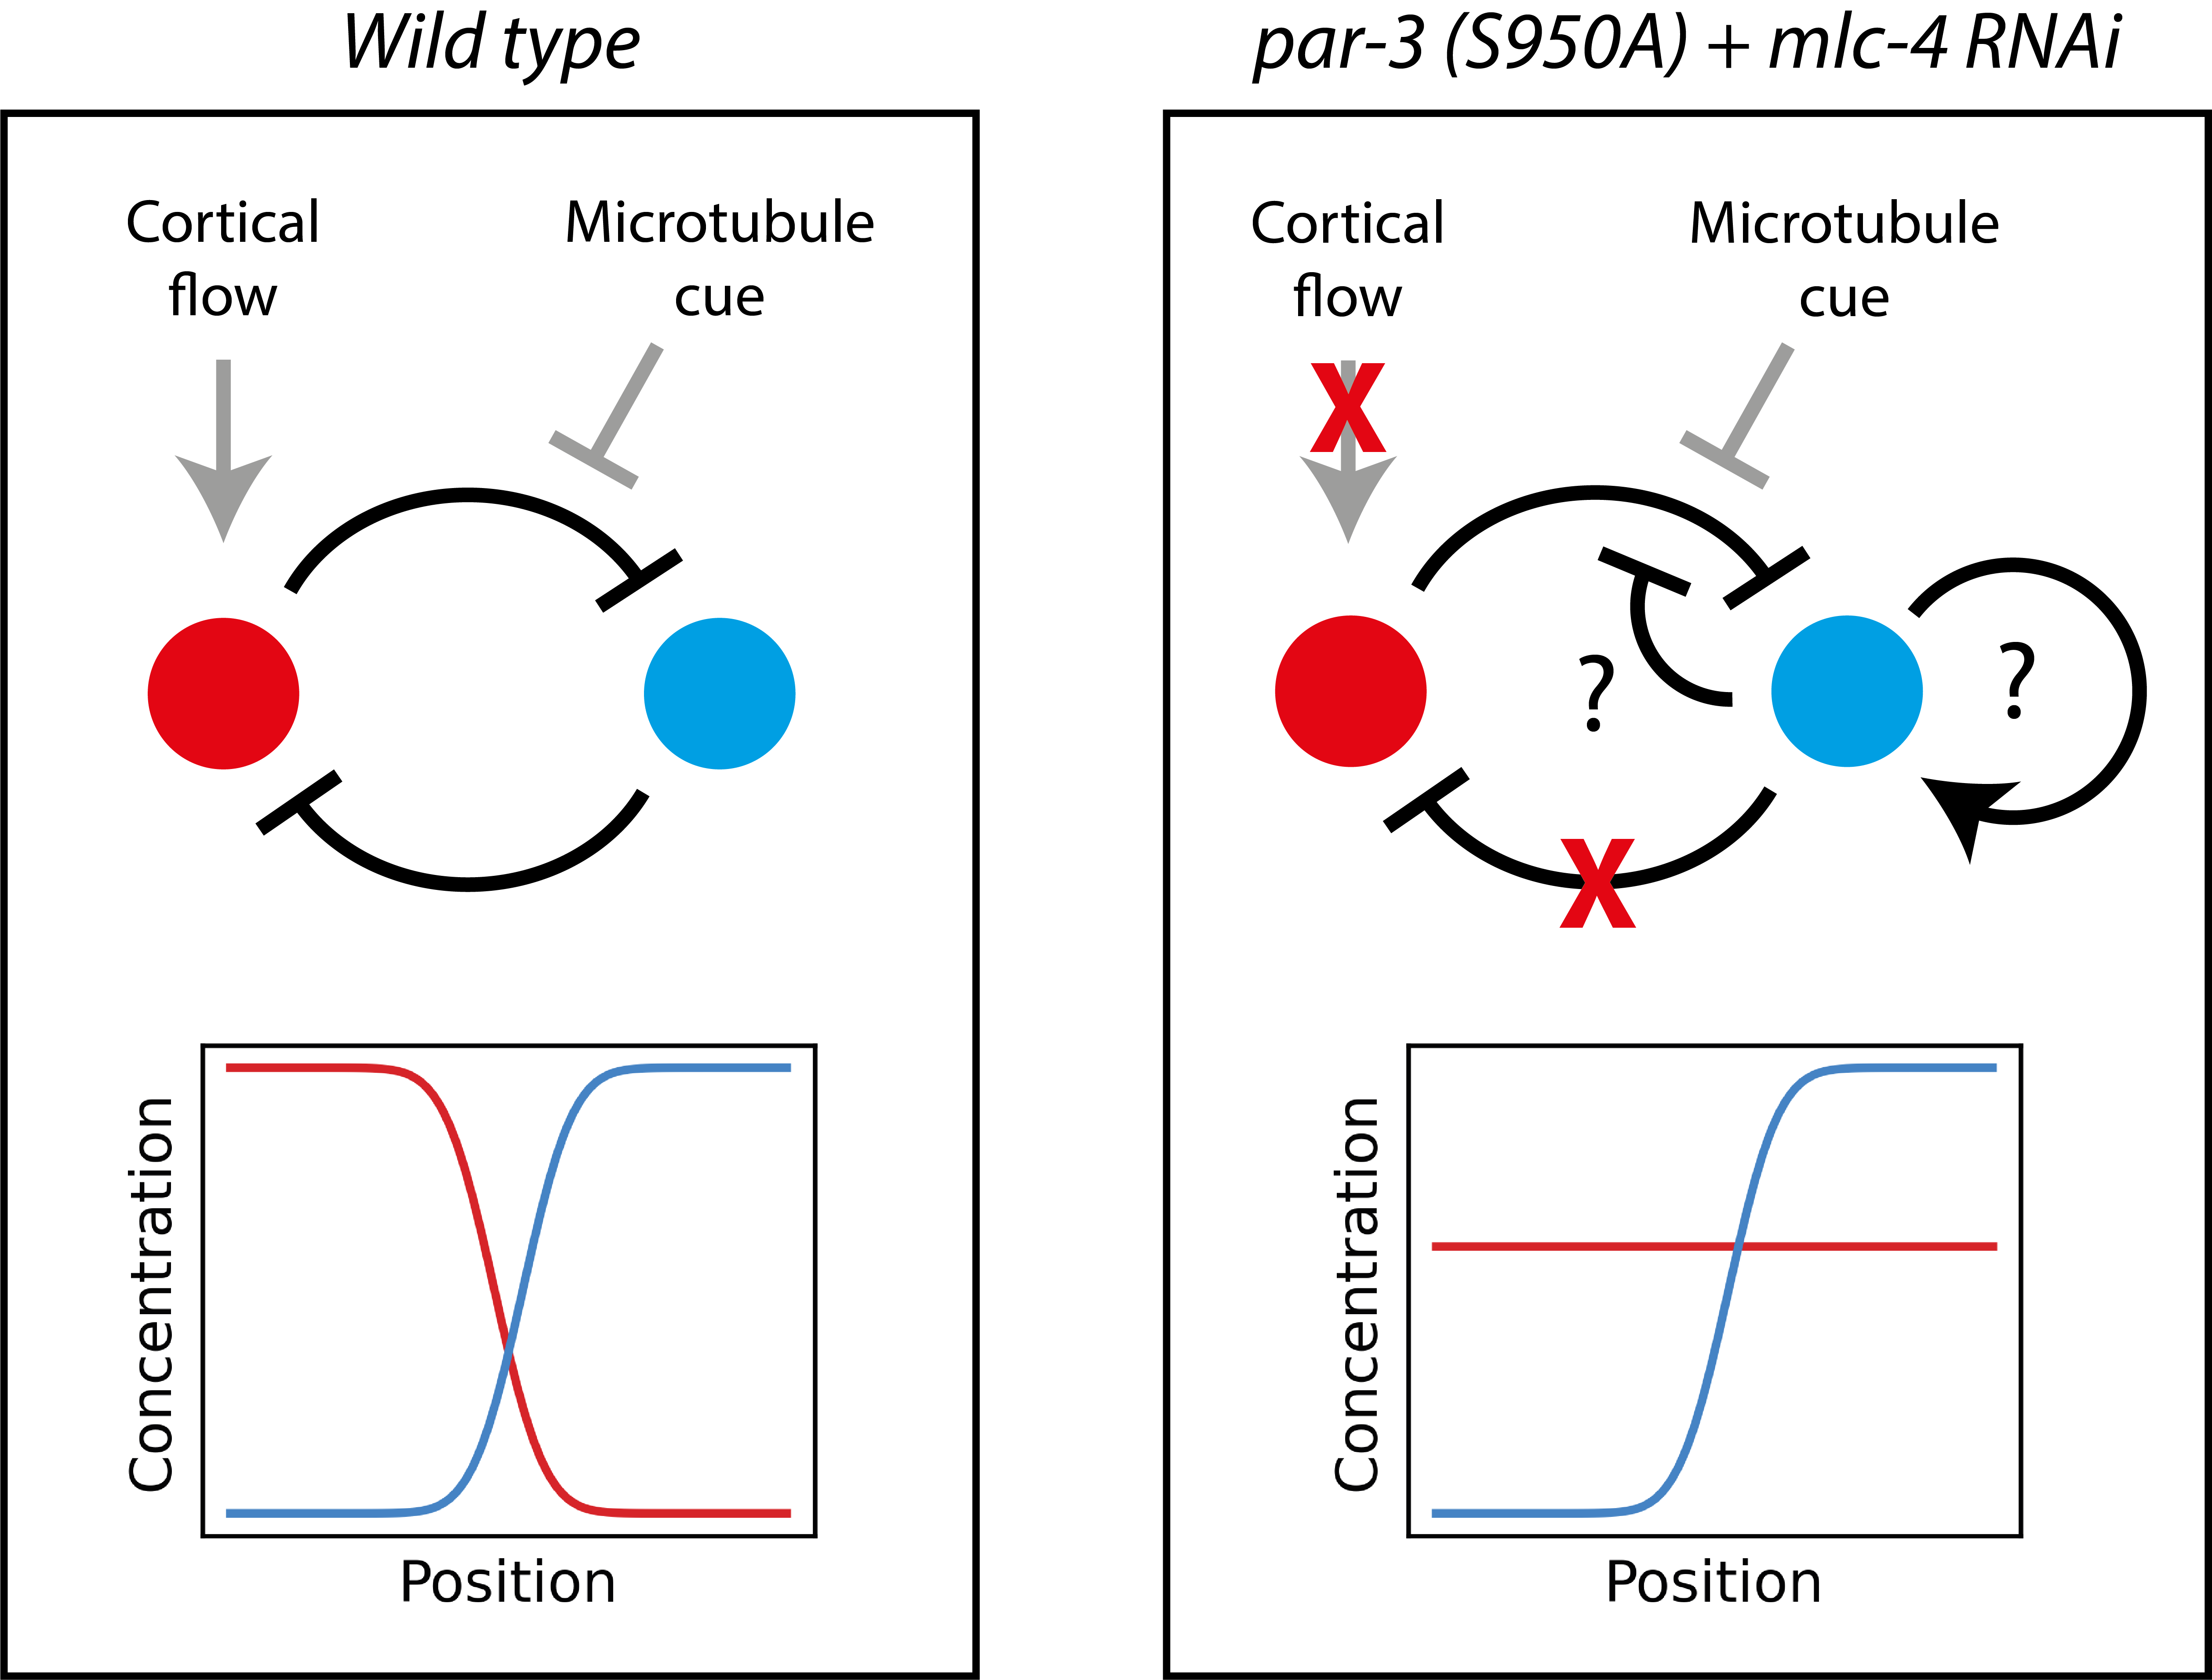
\includegraphics[scale=1.1]{polarity_regimes_schematics}
\centering
\mycaption{Schematic of pPAR polarity in systems with uniform aPAR}{
In systems lacking cortical flows (e.g. \textit{mlc-4 RNAi}) and lacking pPAR to aPAR feedback (e.g. \textit{par-3 (S950A), par-1 RNAi}), aPARs fail to polarise. Nevertheless, PAR-2 is still able to polarise under these conditions, implying the existence of additional feedback reactions. Possible reactions that have been proposed include a positive feedback reaction in which cortical PAR-2 can self-recruit cytoplasmic PAR-2, an inhibitory reaction from PAR-2 to PKC-3 activity, or entry of PAR-2 into a PKC-3 resistant state. The distribution of other pPARs (LGL-1, CHIN-1) in this state is unknown. Black arrows represent feedback reactions. Spatial cues (grey arrows) are active during symmetry breaking but dissipate during maintenance phase.
}
\label{fig:polarity_regimes_schematics}
\end{figure}


\subsection{Self-recruitment}

Using an in vitro microtubule pelleting assay, along with analysis of truncation mutants, \textcite{Motegi2011} were able to identify the regions of PAR-2 responsible for microtubule binding. Two independent mutations to basic residues within these regions (R163A and R183-5A, \ref{fig:par2_schematic}) were found to reduce the level of microtubule binding in vitro, and prevent symmetry breaking in no-flow conditions in vivo. Interestingly, whilst these mutants are usually unable to access the cortex in conditions with uniform aPAR, they can do so when wild-type PAR-2 is also present. This has led to proposals that PAR-2 may have the ability to self-recruit, meaning that cortical PAR-2 molecules may recruit additional cytoplasmic PAR-2 molecules to the cortex. In line with this, PAR-2 has been shown to self-associate in in vitro pull-down assays \citep{Motegi2011, Arata2016}.\\

\textcite{Arata2016} expanded on this by showing that PAR-2 exists as oligomers at the cortex. By TIRF imaging, the authors were able to resolve distinct PAR-2 particles of varying size at the cortex, which showed a slight asymmetry towards larger oligomers at the posterior. Membrane lifetime was found to vary across the cell according to oligomer size and local PKC-3 concentration, indicating that oligomerisation can increase, and phosphorylation decrease, the stability of membrane binding. They also found an asymmetry in the membrane association rate, highest in the posterior of polarised cells, which they suggest could be due to direct recruitment of cytoplasmic PAR-2 into cortical oligomers.\\

Self-recruitment may lead to a positive feedback reaction, whereby cytoplasmic PAR-2 is preferentially recruited to regions of high cortical PAR-2. Such a reaction may allow the PAR-2 domain to independently grow and self-stabilise, even in the presence of a uniform antagonist. However, the extent to which this reaction impacts the membrane binding kinetics of PAR-2 is not understood, and we lack quantitative data to assess the strength and significance of this feedback. \\


\subsection{RING domain}

Studies of mutant PAR-2 alleles have demonstrated an important role for the N-terminal RING domain in establishing strong PAR-2 domains. Under normal conditions, RING mutant PAR-2 (C56S) can form a posterior polarity domain following aPAR advection, but this domain is weakly concentrated compared to wild type PAR-2 \citep{Hao2006}. Following cessation of flows at maintenance phase, aPARs spread back towards the posterior, causing the PAR-2 domain to be largely cleared by the time of cytokinesis. This implies that RING-mutant PAR-2 domain lacks the fundamental properties of wild type PAR-2 domains that allow them to overcome antagonism from PKC-3. In no-flow conditions PAR-2 C56S remains entirely cytoplasmic and unable to trigger formation of a domain \citep{Motegi2011}. Whilst it is clear that the RING plays a significant role in organising the PAR-2 domain, insight into the mechanisms of RING domain action is lacking. The extent to which the RING phenotype is a consequence of intrinsically lower membrane affinity, failures in the self-recruitment pathway described above, or a represents a specific role for the RING domain in counteracting PKC-3 (e.g. by making the protein a poorer substrate) is unclear.\\

\begin{figure}
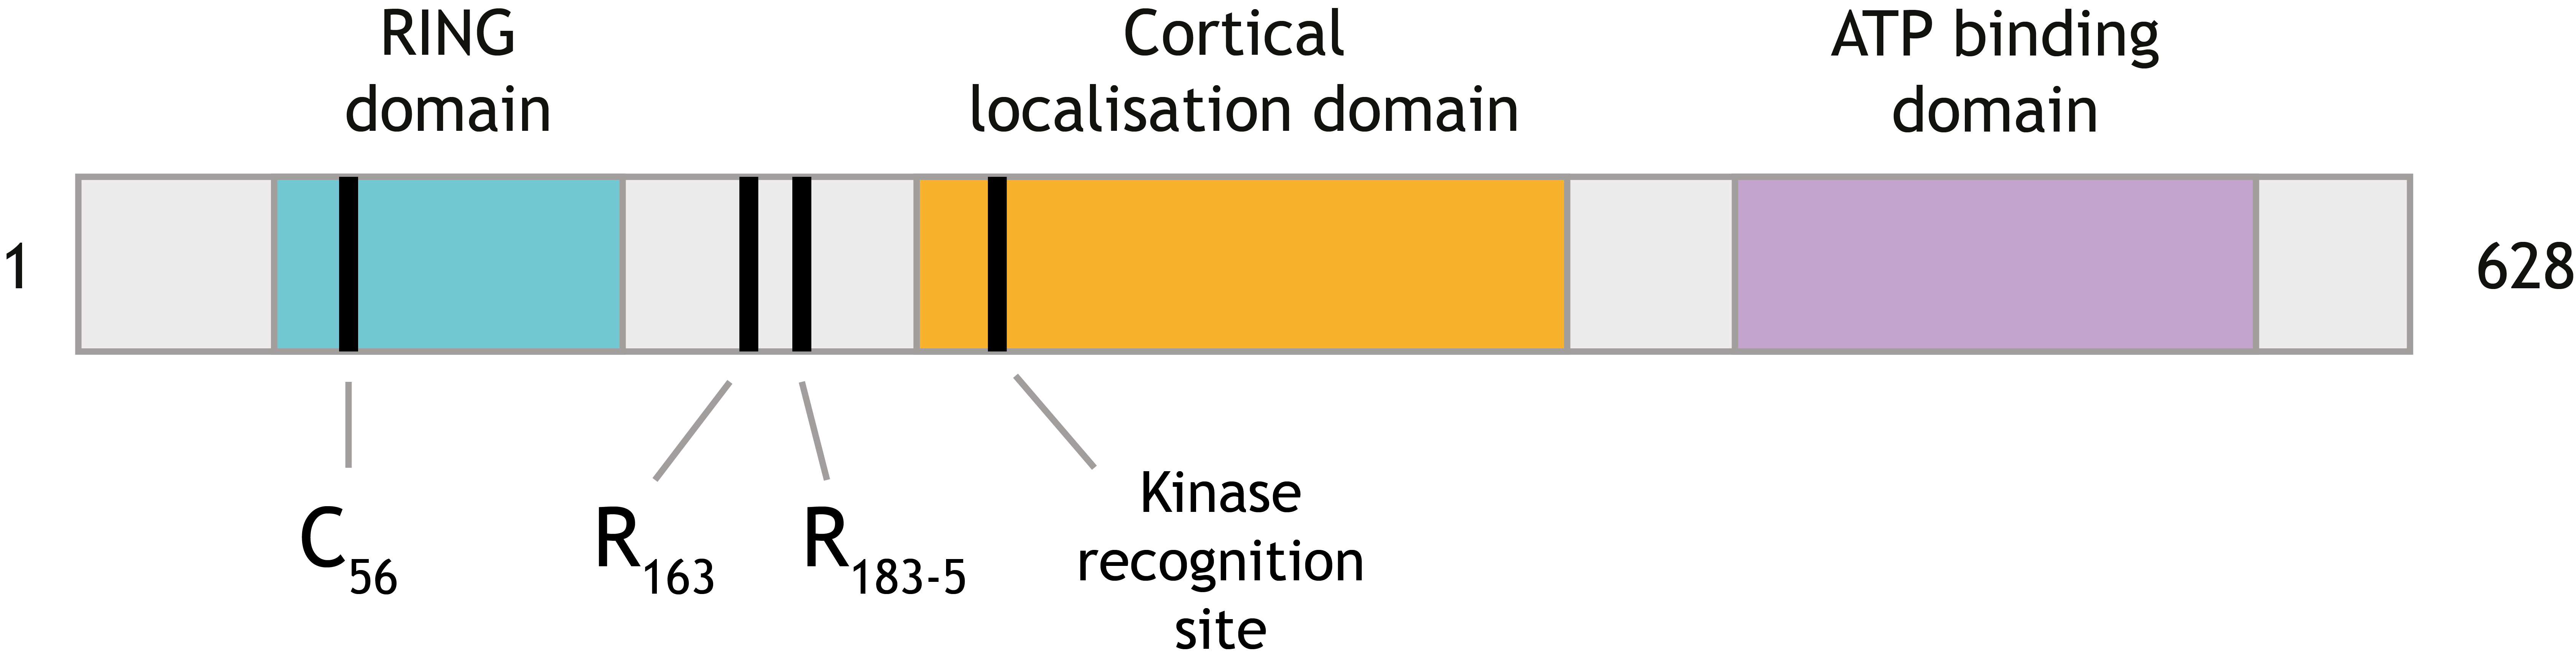
\includegraphics[scale=0.95]{par2_schematic}
\centering
\mycaption{Schematic representation of PAR-2}{
Indicates the position of sites for which mutation disrupts PAR-2 driven polarity in no-flow regimes.
}
\label{fig:par2_schematic}
\end{figure}

\subsection{Substrate-kinase interaction}

Unpublished work by Florent Peglion (Goehring lab) has shown that a mutant PAR-2 allele with a weakened PKC-3 recognition motif (identified as the AxA mutant), whist able to polarise relatively normally in wild type backgrounds, is unable to drive polarity in no-flow conditions. A possible interpretation of this result is that the ability for PAR-2 to resist PKC-3 might, perhaps counterintuitively, rely on tight association between PAR-2 and the kinase. Whilst intermediate substrate affinity is often compatible with efficient enzymatic activity, high substrate affinity can lead to a stable interaction between kinase and substrate which can effectively block enzymatic activity. PAR-3, which has a similar PKC-3 recognition site to PAR-2, can act as either a substrate or an inhibitor of PKC-3 depending on its affinity, which is under regulatory control \citep{Soriano2016}. In the case of PAR-2, regulation of binding affinity to PKC-3, perhaps via nonlinear concentration-dependent behaviours, may underlie its ability to resist antagonism in some contexts, whilst being sensitive in other contexts. Work to uncover the nature of the PAR-2/PKC-3 interaction is ongoing in the Goehring lab.\\

% Personaly I think that, whilst there's probably something interesting here, there might be a more obvious way to explain the AxA phenotype which is that PAR-2 is uniformly on the cortex at a higher level than wild type at symmetry breaking, so cytoplasmic concentrations presumably lower, so probably harder to respond to any cues. Had a quick look at Florent's data and this appears to be the case.

\subsection{Outlook}

Overall, this work paints a picture of PAR-2 polarity that extends beyond the mutual antagonism model. Whilst under normal conditions, advective transport and mutual antagonism may dominate the patterning process, the secondary microtubule-dependent pathway appears to rely, at least partially, on feedback reactions intrinsic to PAR-2 itself. Following initial recruitment to the cortex by microtubules, self-recruitment of PAR-2 molecules from the cytoplasm enhances cortical PAR-2 concentrations. Diffusive spread, along with the ability to resist PKC-3 when highly concentrated allows PAR-2 to spread anteriorly and rapidly invade cortical space occupied by aPAR. At the same time, cortical PAR-2 recruits PAR-1 from the cytoplasm. By phosphorylating PAR-3, PAR-1 eventually clears aPARs from the posterior, restricting them to the anterior.\\

However, our understanding of this process is far from complete. Primarily, whilst feedback pathways have been proposed, we lack insight into the quantitative nature of these pathways, which limits our ability to understand the system with computer models. Furthermore, we lack good insight into the quantitative characteristics of PAR-2 mutants, including basic properties such as membrane affinities and total protein levels, which complicates interpretation of phenotypes. Recent advances in techniques for in vivo quantification, described in the previous chapter, overcome some of these barriers and should enhance our ability to obtain accurate quantitative data. \\

Additionally, previous studies are complicated by their reliance on transgenic lines. As expression of PAR-2 transgenes is not under the same regulatory control as endogenous PAR-2, and the location of transgene insertions in the genome varies from line to line, protein levels are often not comparable to endogenous protein levels, and can strongly differ between lines. This is a potential concern, as the ability for PAR-2 to polarise in no-flow conditions is sensitive to small changes in PAR-2 amounts (Rodrigues). Recent advances in CRISPR technologies mean that we can now tag and monitor endogenous PAR-2 with relative ease, which may control for this potentially confounding factor.\\

% Might be worth having a section here where I confirm the phenotypes of the mutants in CRISPR lines (i.e that they can't break symmetry in no-flow). I have a good dataset for the microtubule mutants but not wild type or C56S. Florent has some data for AxA but I would want to redo if its also worth including.

\section{Quantitative characterisation of PAR-2 mutant alleles}

With this in mind, my first aim was to perform quantitative analysis of the membrane binding behaviour of PAR-2 and the mutant alleles described previously for which polarity-defective phenotypes have been reported (R163A, R183-5A, AxA and C56S). By CRISPR to an endogenously tagged GFP::PAR-2 line, we created a series of point mutants at the endogenous \textit{par-2} locus (\cref{fig:par2_misc_mutants_quantification}A). In order to separate intrinsic and PKC-3 dependent behaviours, I crossed each line to a line expressing the \textit{par-3 (it71)} allele, a nonsense mutation in which shows no detectable protein in early embryos \citep{Etemad-Moghadam1995}. Consequently, PKC-3 remains cytoplasmic and inactive, and PAR-2 binds uniformly to the cortex (\cref{fig:par2_misc_mutants_quantification}B). Using the protocol described in the section 2 involving autofluorescence correction and computational separation of membrane and cytoplasmic signal components, I performed full quantitative analysis of each line. In \cref{fig:par2_misc_mutants_quantification}C and D I present quantifications of membrane to cytoplasmic ratios, a measure of membrane affinity. Fig \ref{fig:par2_misc_mutants_detailed_quantification} shows full quantification results, including cytoplasmic concentrations, membrane concentrations and total protein levels.\\

As expected, whilst PAR-2 AxA behaves differently to wild type PAR-2 in polarised cells, owing to its weaker interaction with PKC-3, membrane affinity in \textit{par-3 (it71)} cells is equal to wild type, suggesting that the mutant harbours no intrinsic defect in membrane binding.\\

PAR-2 C56S, by contrast, has a membrane affinity greatly reduced compared to wild type. This is the case even in \textit{par-3 (it71)} mutants, suggesting that the localisation defect is intrinsic to PAR-2, rather than via hypersensitivity to PKC-3 as has previously been suggested \citep{Hao2006}. Overall protein levels are also slightly reduced compared to wild type (\cref{fig:par2_misc_mutants_detailed_quantification}A and D). This is in contrast to previous results using transgenic lines which showed higher levels in RING mutants. The reason for this discrepancy is unclear, but I believe that in this case the small reduction in expression compared to wild type may relate to protein instability caused by unfolding of the RING domain.\\

Surprisingly, I found that the microtubule-binding mutants (R163A and R183-5A) also have weaker membrane affinities compared to wild type PAR-2. This is independent of aPARs, suggesting that the defect is intrinsic to PAR-2. Such a defect has previously not been reported in studies using these lines \citep{Motegi2011, Gross2018}. These mutants also have a mild overexpression phenotype. As a result, membrane concentrations are similar to wild type concentrations despite the reduction in membrane to cytoplasmic ratio.\\

\begin{figure}
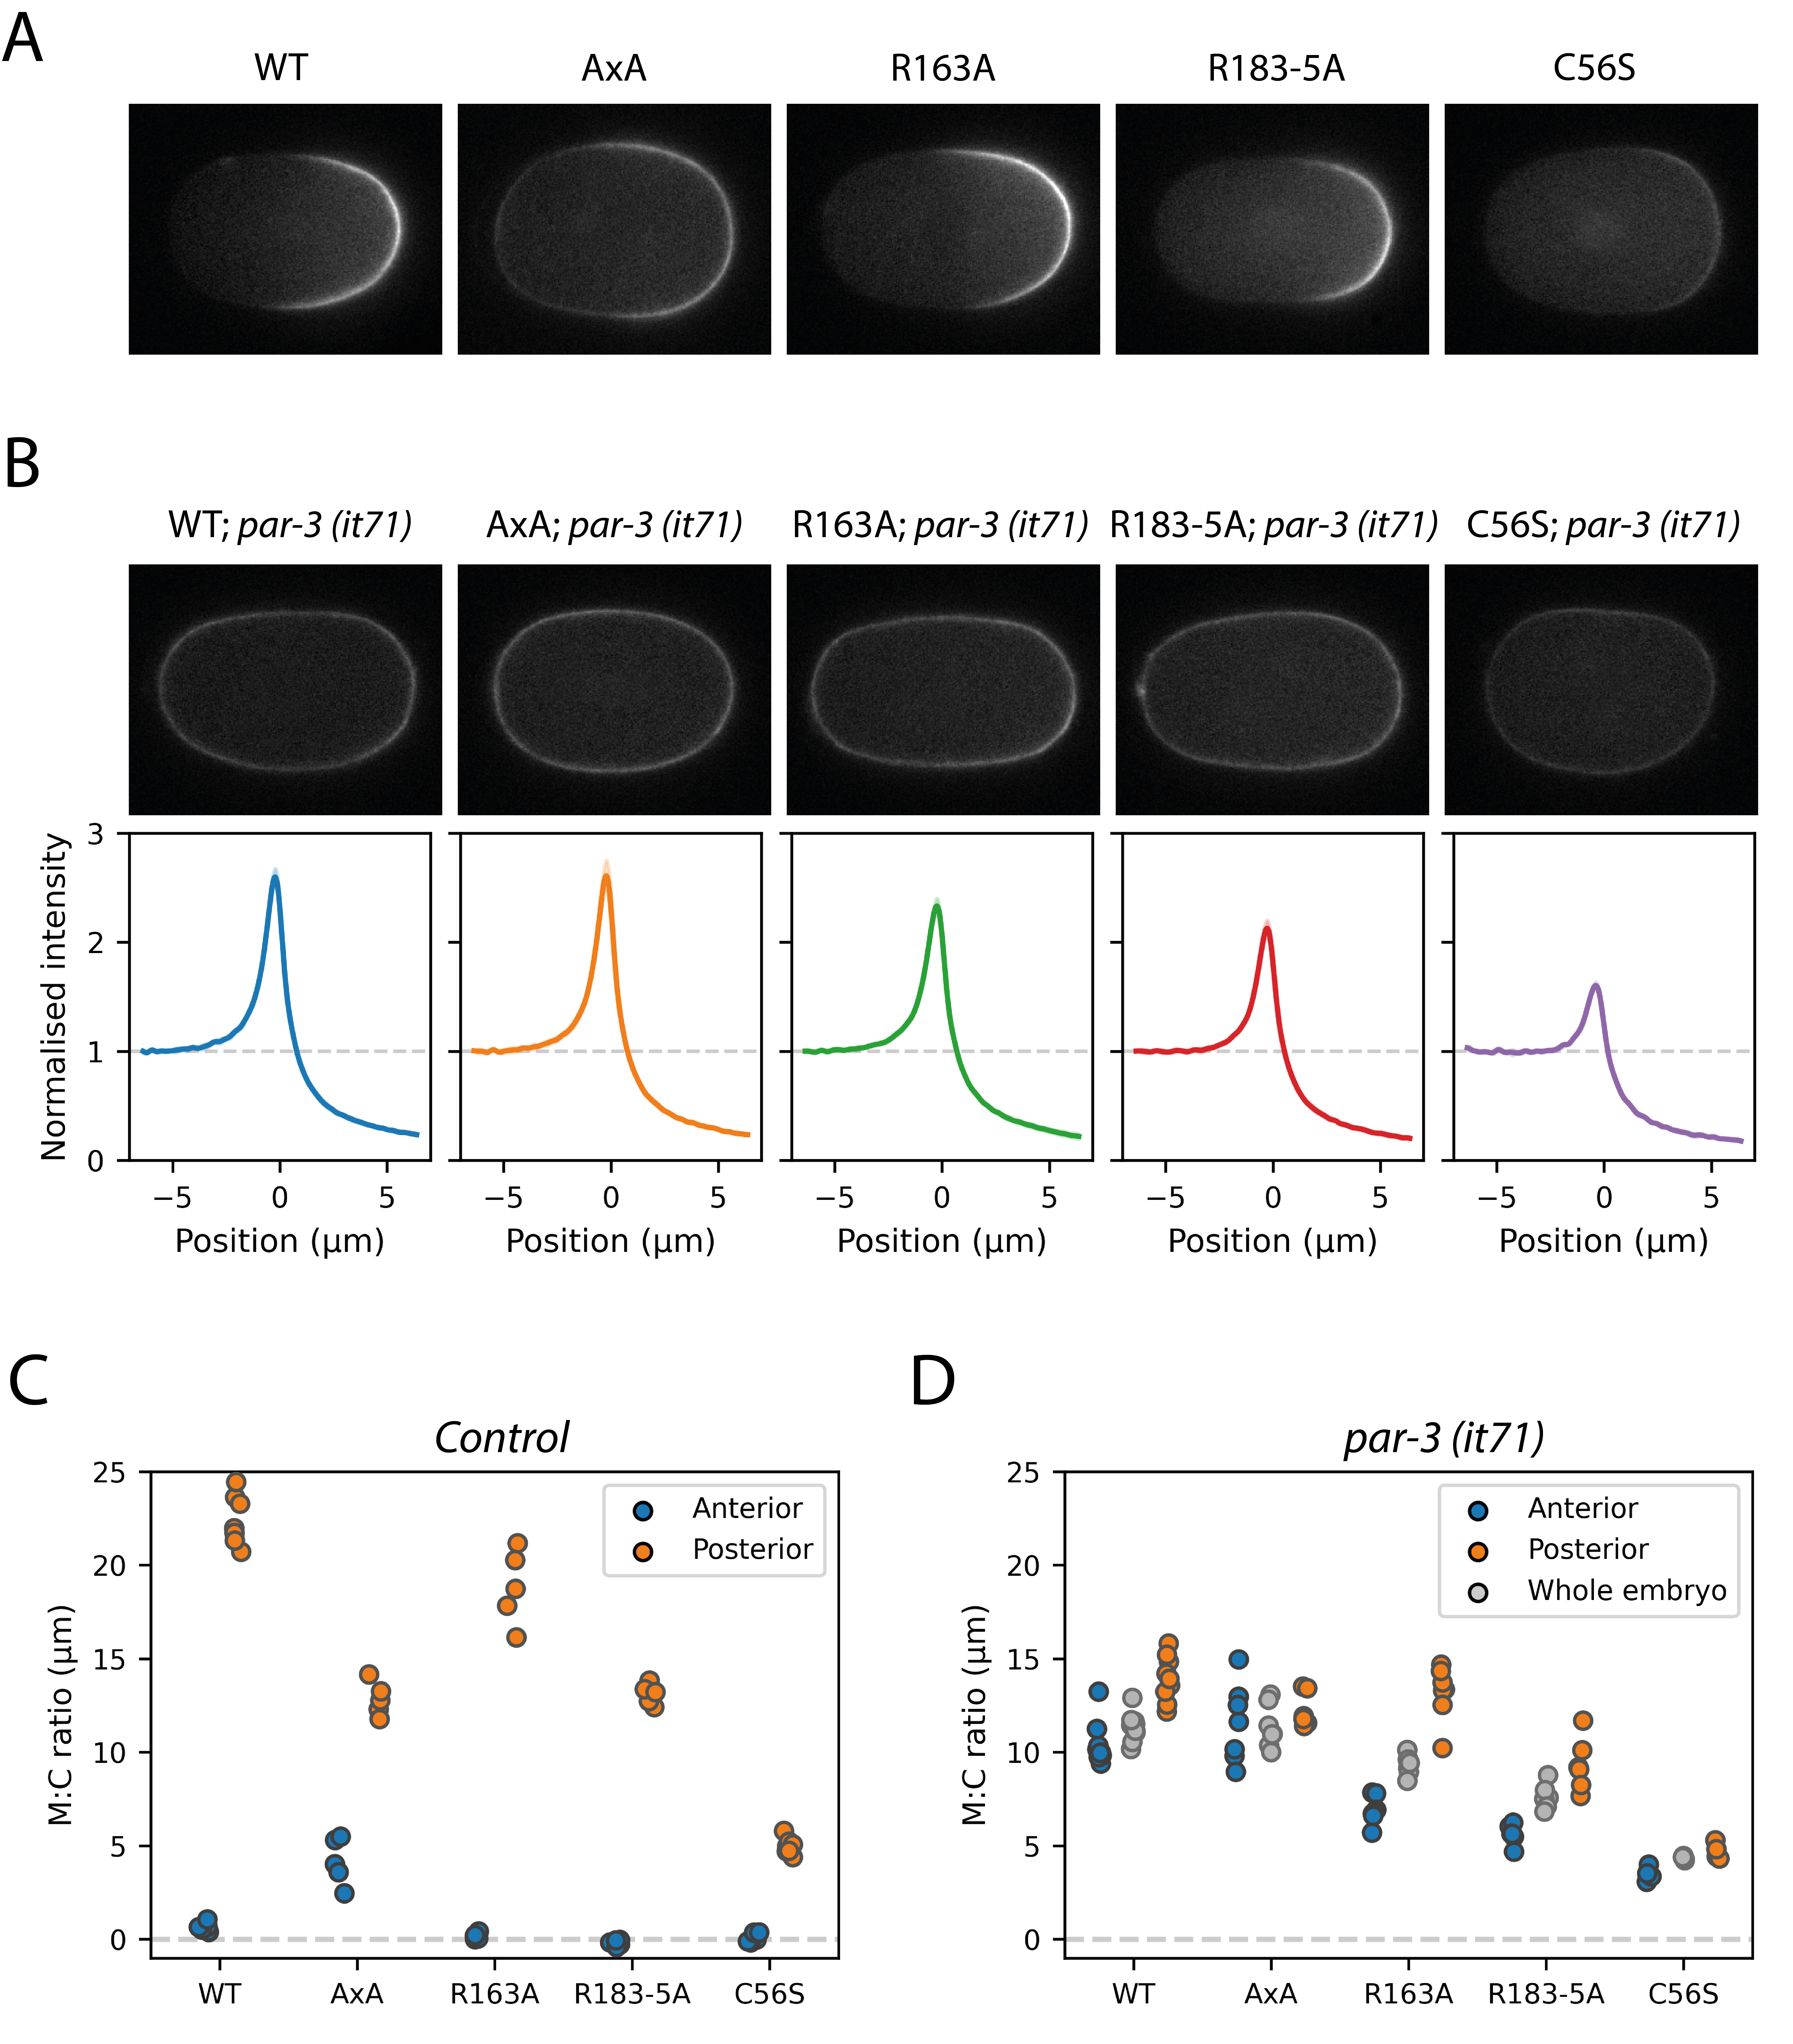
\includegraphics[scale=1]{par2_misc_mutants_quantification}
\centering
\mycaption{Membrane affinities of wild-type PAR-2 and mutant alleles in polarised and uniform systems}{
\textbf{(A)} Midplane confocal images of GFP::PAR-2 (wt) and mutant alleles in polarised cells (\textit{par-3 (wt)}) at maintenance phase.
\textbf{(B)} Midplane confocal images of GFP::PAR-2 (wt) and mutant alleles in uniform cells lacking functional aPAR (\textit{par-3 (it71)}). Bottom panels show normalised cross cortex profiles around the entire circumference of the embryo, averaged over all embryos in the dataset (mean $\pm$ SD).
\textbf{(C)} Quantifications of membrane to cytoplasmic ratio for the five PAR-2 alleles in control (\textit{par-3 (wt)}) zygotes. Shows ratios averaged over the anterior and posterior 20\% of the zygote.
\textbf{(D)} Quantifications of membrane to cytoplasmic ratio for the five PAR-2 alleles in uniform (\textit{par-3 (it71)}) zygotes. Shows ratios averaged over the anterior and posterior 20\% of the zygote, and averaged over the whole zygote. All images were taken at NEBD.
}
\label{fig:par2_misc_mutants_quantification}
\end{figure}

\begin{figure}
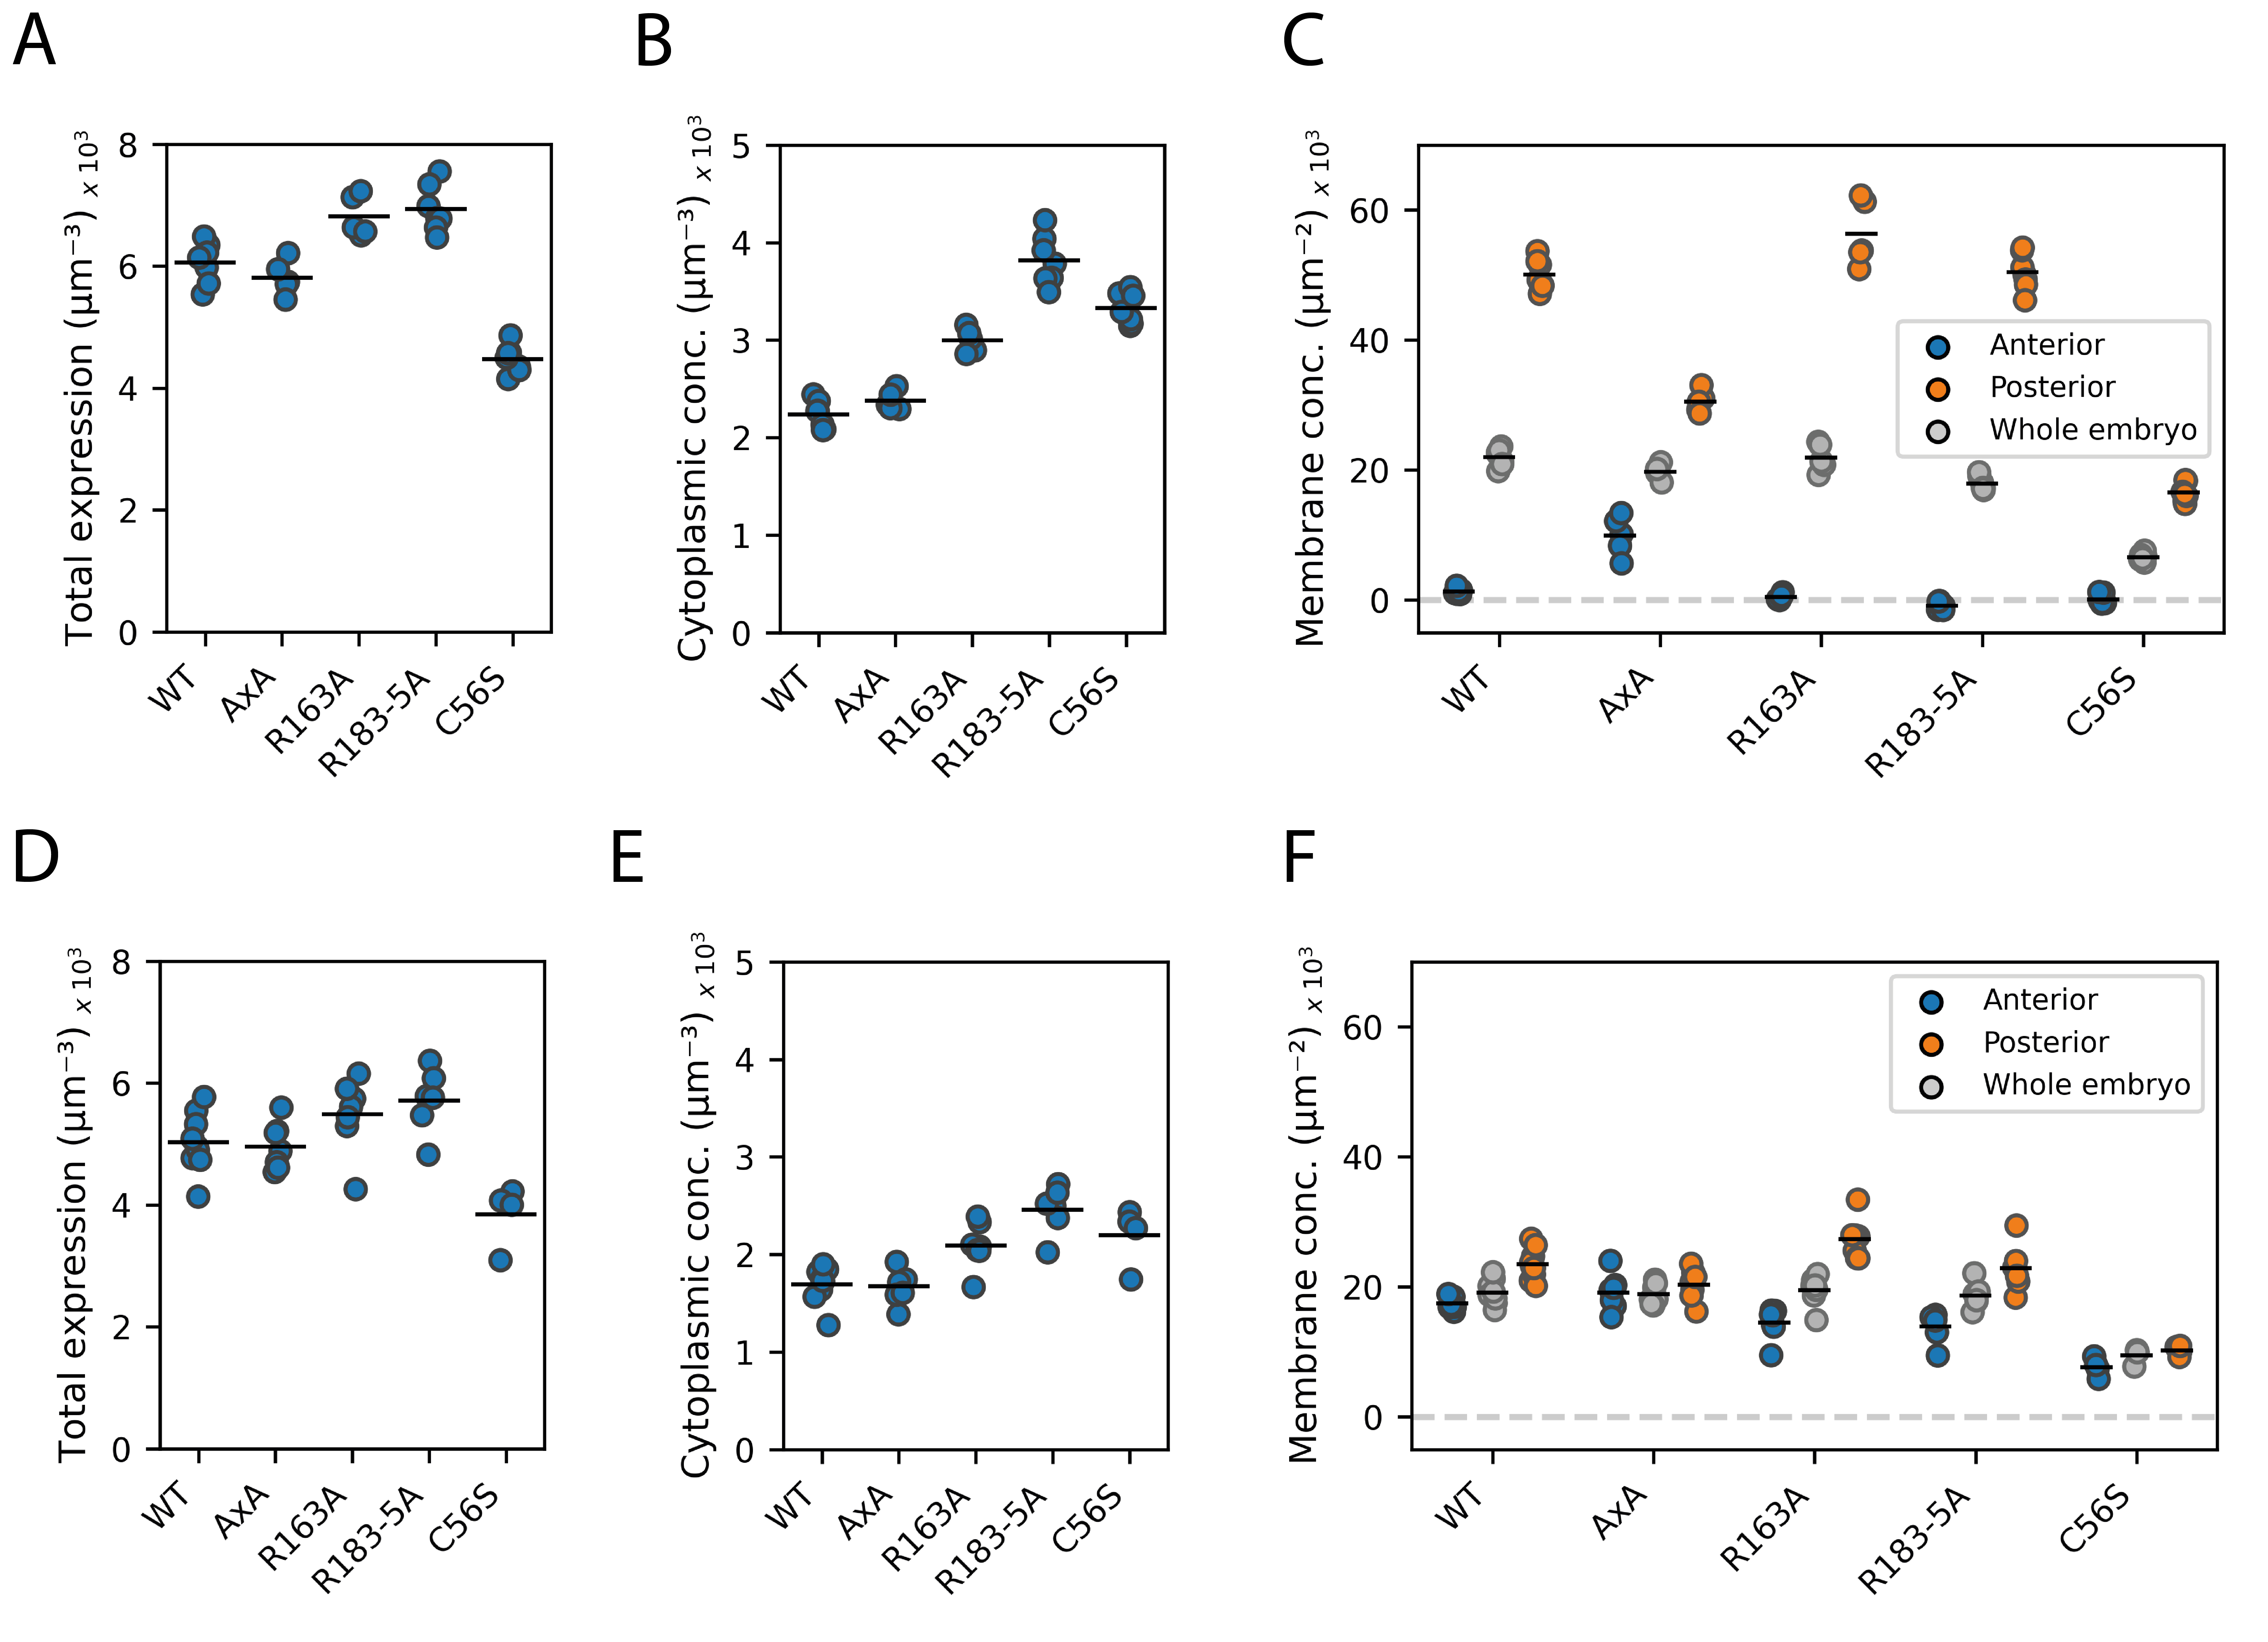
\includegraphics[scale=0.9]{par2_misc_mutants_detailed_quantification}
\centering
\mycaption{Further quantification of wild-type PAR-2 and mutant alleles in polarised and uniform systems}{
\textbf{(A) - (C)} Quantification of total expression (A), cytoplasmic concentration (B) and membrane concentrations (C) for wild type and mutant GFP::PAR-2 in polarised cells (\textit{par-3 (wt)}). 
\textbf{(D) - (F)} Quantification of total expression (D), cytoplasmic concentration (E) and membrane concentrations (F) for wild type and mutant GFP::PAR-2 in uniform cells (\textit{par-3 (it71)}). 
}
\label{fig:par2_misc_mutants_detailed_quantification}
\end{figure}


% Not sure whether the AxA data adds much and might take away the focus a bit. I'm mainly just including it because I have the data. For the paper, we will probably want to leave out AxA anyway as this mutant isn't published yet


\section{RING domain promotes positive feedback to achieve optimal membrane affinity}
\label{section:par2_rundown}

Whilst membrane concentrations are expected to be higher in polarised cells than uniform (\textit{par-3 (it71)}) cells due to an increase in the concentration of the cytoplasmic pool, membrane affinity, which is a simple function of membrane binding and unbinding rates, is expected to be constant. In other words, the membrane and cytoplasmic concentrations of a protein undergoing membrane exchange with constant binding and unbinding rates should fall along a linear trajectory (\cref{fig:rundown_schematic}A).\\

For wild type PAR-2, this doesn't appear to be the case. Transition from a polarised system to a uniform system leads to a modest drop in cytoplasmic concentrations, but a comparatively large drop in membrane concentrations, and consequently a drop in membrane to cytoplasmic ratio (\cref{fig:par2_misc_mutants_quantification} and \ref{fig:par2_misc_mutants_detailed_quantification}). This implies that the membrane environment is different in polarised cells, such that the membrane binding rate is higher, or the membrane unbinding rate lower, than in a uniform system.\\

Given previous proposals that PAR-2 may be able to self-recruit, I reasoned that such a reaction may be behind this deviation from expected default kinetics. A positive feedback reaction, whereby PAR-2 promotes its own recruitment to the membrane, may be expected lead to a nonlinear relationship between membrane and cytoplasmic concentrations if feedback is sufficiently strong. The expected shape of the relationship depends on the strength and form of positive feedback. In the simplest case, positive feedback can increase membrane affinity as a function off membrane concentration, such that the gradient of the cytoplasm vs membrane relationship will be higher at higher membrane concentrations (\cref{fig:rundown_schematic}B). Under some parameter regimes, nonlinear feedback may lead to bistability, whereby multiple membrane concentrations can be supported within a range of cytoplasmic concentrations (\cref{fig:rundown_schematic}C). A reaction like this is, in theory, sufficient for polarity in the absence of any additional spatial information, and has been proposed for models involving Rho-GTPases in yeast \citep{Mori2008}.\\

\begin{figure}[!h]
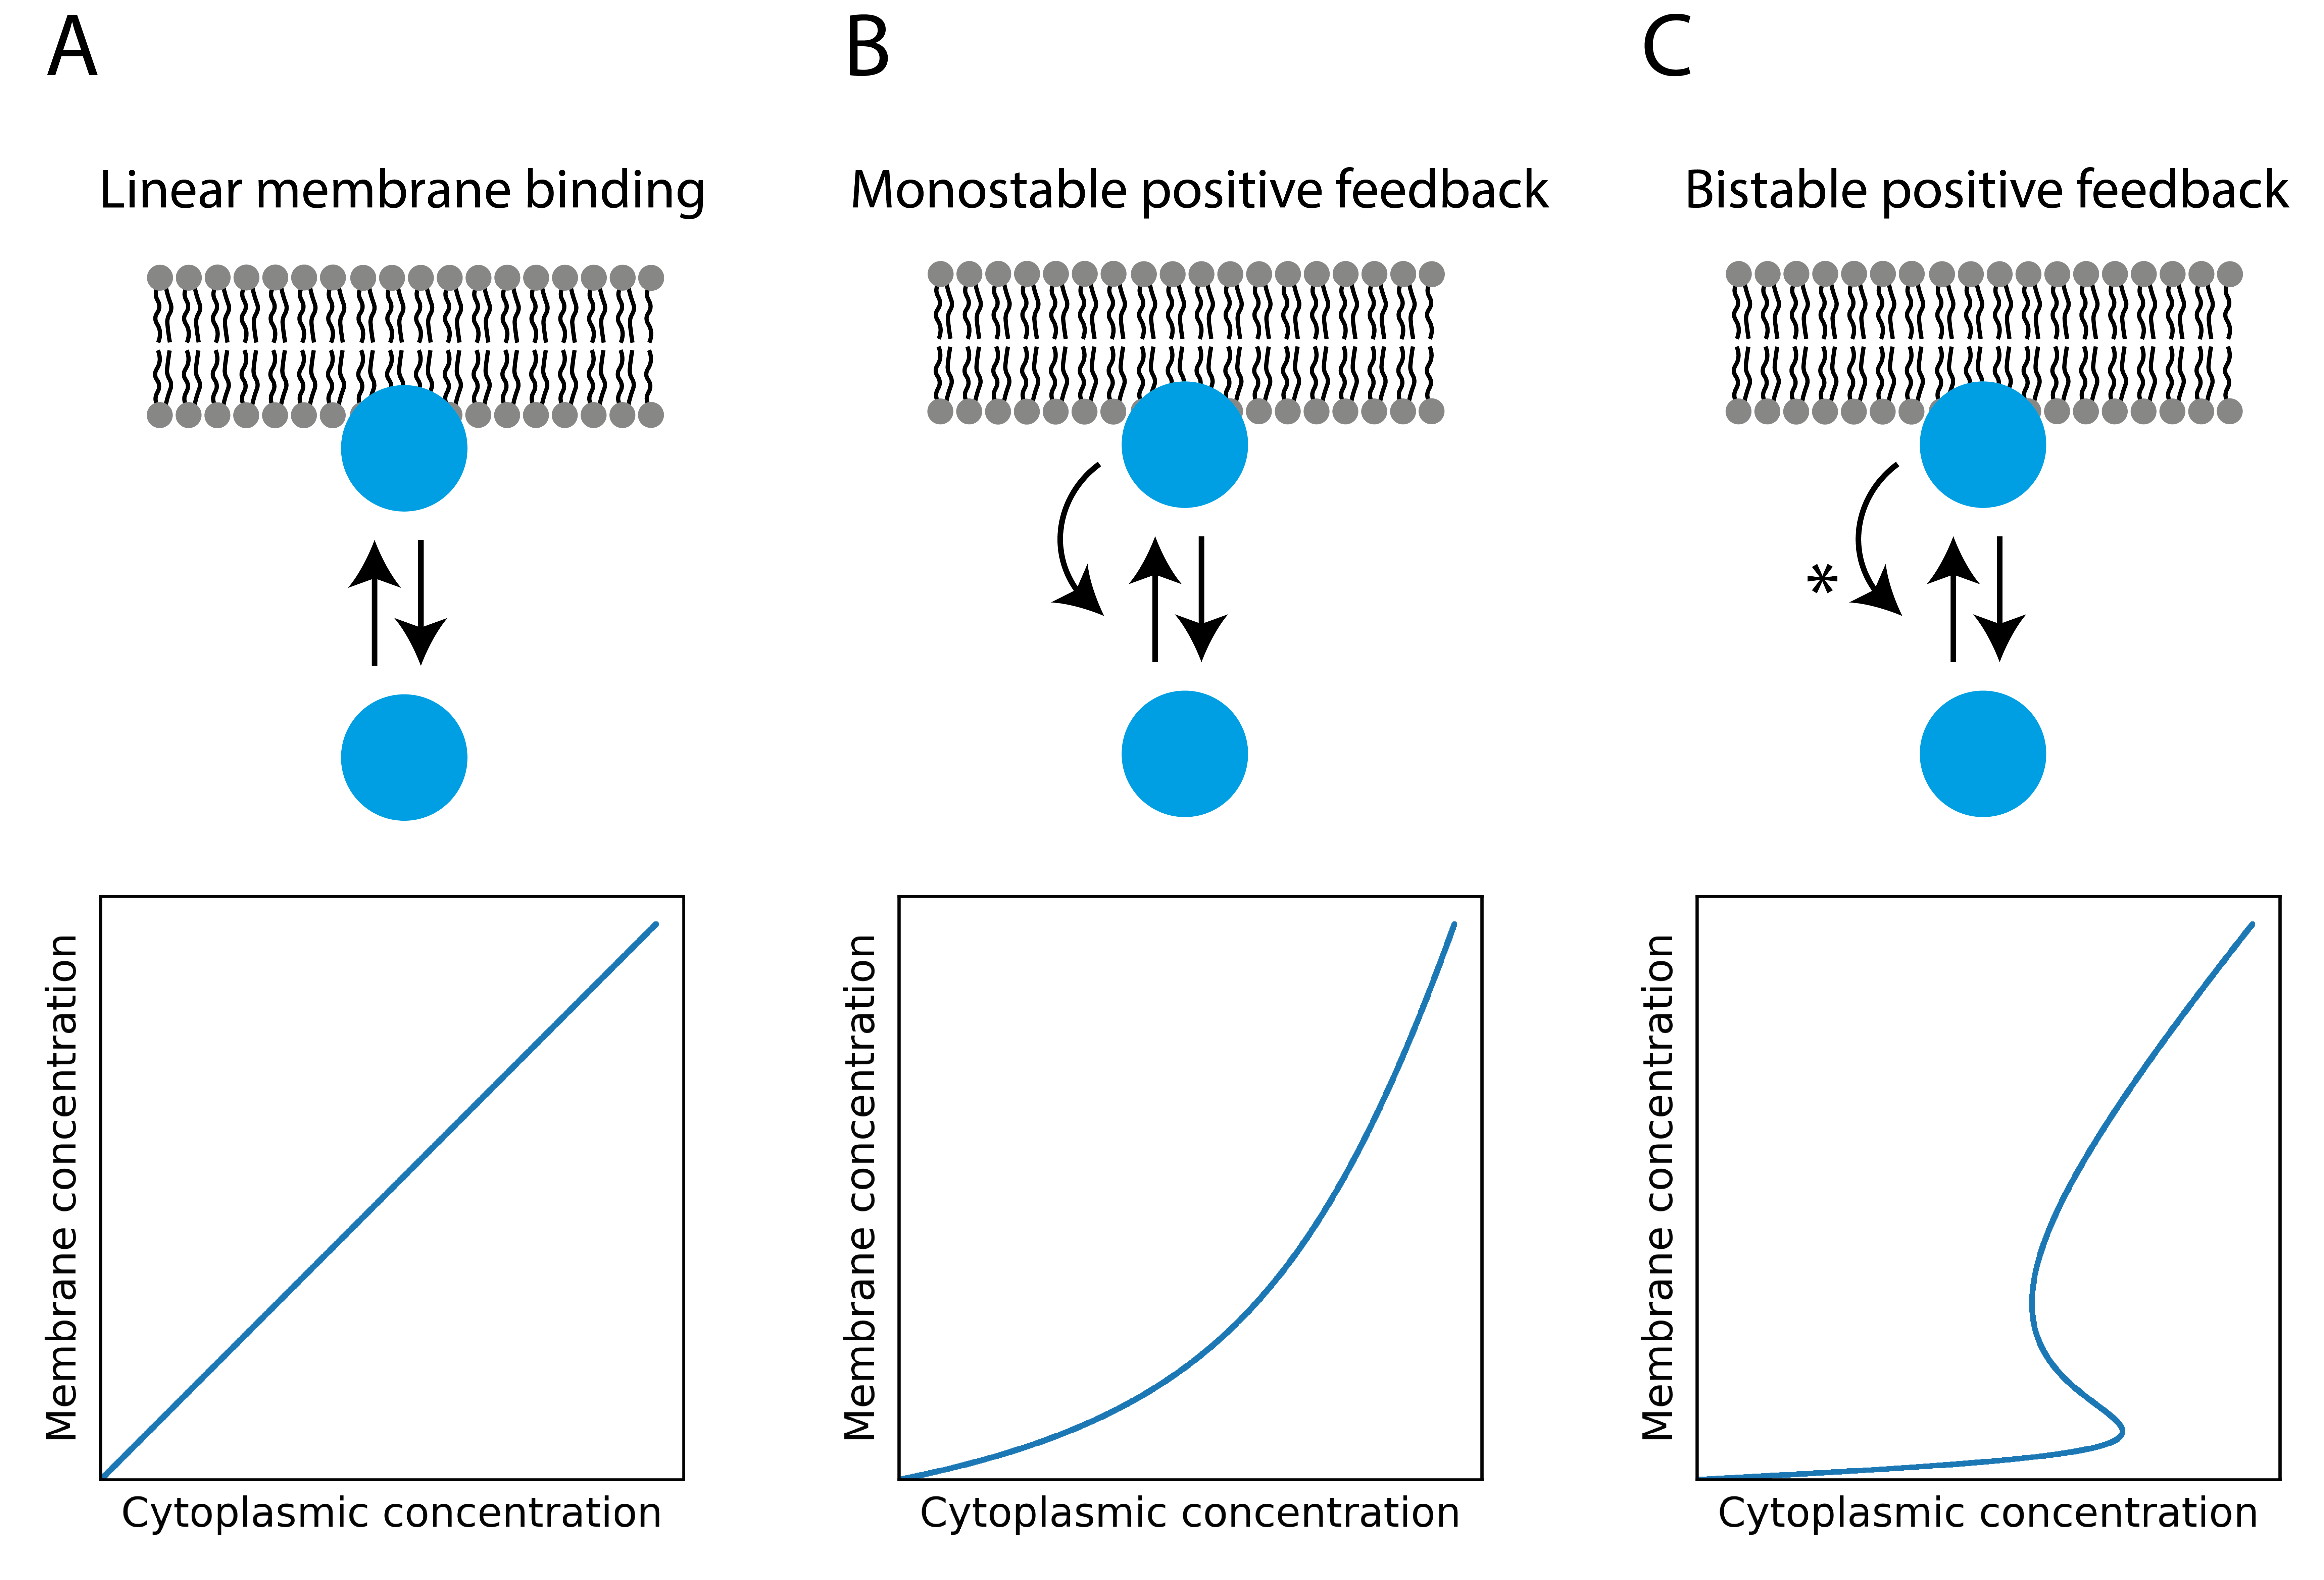
\includegraphics[scale=0.95]{rundown_schematic}
\setlength{\abovecaptionskip}{20pt}
\centering
\mycaption{Cytoplasm versus membrane relationships for models with and without positive feedback}{
A protein exchanging between the membrane and cytoplasm with constant on and off rate kinetics is expected to show a linear relationship between cytoplasmic and membrane concentrations (A).
A protein feeding back onto it's own membrane recruitment is expected to have a nonlinear relationship (B).
Where feedback is nonlinearly dependent on membrane concentrations (asterix), bistability can exist under some parameter regimes, whereby multiple membrane concentrations can be supported within a range of cytoplasmic concentrations (C).
ODEs were build using a constant off rate term ($k_{off} = 1$), with on rates specified by the following terms for the three models: (A) $k_1$ (B) $k_2 + \frac{k_3 M}{k_4 + M} $ (C) $k_5 + \frac{k_6 M^2}{k_7^2 + M^2}$ where $k_1 = 1$, $k_2 = 0.05$, $k_3 = 1$, $k_4 = 1$, $k_5 = 0.05$, $k_6 = 1$, $k_7 = 1$ and $M$ is the membrane concentration, and solved for membrane and cytoplasmic concentrations at steady state. 
}
\label{fig:rundown_schematic}
\end{figure}

In a \textit{par-3 (it71)} background, a PAR-2 intrinsic positive feedback reaction implies that cytoplasmic and membrane concentrations should vary nonlinearly in cells with varying quantities of PAR-2. A commonly used method that can be used to vary protein amounts in \textit{C. elegans} is RNAi, which reduces protein amounts in a manner that can be tuned by duration of dsRNA exposure. To test for the existence of PAR-2 intrinsic positive feedback, I performed an in vivo titration assay using \textit{par-3 (it71)} mutant worms expressing mNG::PAR-2 (wt), in which I used RNAi to rundown protein levels, and quantified membrane and cytoplasmic concentrations on an embryo-by-embryo basis. mNG (NeonGreen) was selected as a fluorophore as it is significantly brighter that GFP, which aids quantification in cells with long RNAi exposures.\\

Strikingly, the results reveal that PAR-2 doesn't follow strict linear membrane binding kinetics (\cref{fig:rundown_vs_c56s}A, C (blue)). Instead, a nonlinearity appears to be present whereby membrane affinities are higher in cells with higher dosages. The shape of the relationship implies that PAR-2 is feeding back onto its own membrane binding (\cref{fig:rundown_schematic}), but there is no evidence for any discontinuities that would imply bistable behaviour.\\

Interestingly, unlike wild type PAR-2, the membrane affinity of PAR-2 (C56S) is equal in polarised and \textit{par-3 (it71)} systems, despite large changes in membrane and cytoplasmic concentrations. This suggests that the mechanism of positive feedback may be RING-dependent. To test this, I performed a similar titration assay using the PAR-2 (C56S) mutant line. The results (\cref{fig:rundown_vs_c56s}B, C (orange)) show that, the nonlinearity of the cytoplasm vs membrane relationship is greatly reduced compared to wild type, implying that the RING domain may play an active role in promoting positive feedback.\\


\begin{figure}[!h]
\includegraphics[scale=0.88]{rundown_vs_c56s}
\setlength{\abovecaptionskip}{20pt}
\centering
\mycaption{PAR-2 displays RING-dependent nonlinear membrane binding kinetics}{
\textbf{(A) - (B)} Images of \textit{par-3 (it71)} cells expressing wild type (A) or C56S (B) mNG::PAR-2 with varying dosage achieved by \textit{par-2 RNAi}. Bottom panels show mean ($\pm$ SD) normalised cross-cortex intensity profiles for the embryos shown, averaged over the entire embryo circumference.
\textbf{(C)} Quantification of membrane and cytoplasmic concentrations for the full dataset, including untagged N2s (white), which fall close to the origin.
}
\label{fig:rundown_vs_c56s}
\end{figure}

% I know that people will ask where polarised cells fit. For this particular dataset they seem to follow the same trajectory. However, I'm reluctant to include this as it seems to vary between datasets, as we've discussed previously. 

\section{Discussion}

Notes:\\
- Microtubule mutant phenotypes need to be reassessed in light of the quantification results which show that they have a lower membrane affinity than wild type PAR-2\\
- Rundown assay reveals quantitative evidence for PAR-2 positive feedback\\
- Role for RING domain, which will be investigated in the following chapter\\
- Previously, self-recruitment has been suggested to underlie PAR-2's ability to polarise with uniform aPAR. However, my results reveal that this reaction is insufficient to support polarity without additional asymmetries. Suggests that the interaction between PAR-2 and aPARs may also be important, such as an ability to resist or inhibit PKC-3 so that PAR-2 is protected when in a domain\\
- Interaction between PKC-3 and the AxA site may be important. Hopefully will have time to discuss this more in an appendix chapter.\\


%%%%%%%%%%%%%%%%%%%%%%%%%%%%%%%%%%%%%%%%%%%%%%%%%%%%%%%%%%
\clearpage
\chapter{Determining mechanisms of PAR-2 RING domain action}

\textbf{Detailed contributions:}\\

\clearpage
\section{Introduction}

Results in the previous chapter suggest that the RING domain of PAR-2 plays a key role in regulating the membrane affinity of the protein, and may be responsible for conferring nonlinear-membrane binding kinetics to PAR-2. However, the precise mechanisms of RING domain action in this context are not yet understood, and are subject to investigation in this chapter.\\

Whilst no mechanisms have been definitively attributed to the RING domain, several observations in previous studies provide insight into potential mechanisms. On its own, the PAR-2 RING domain has been shown to lack any membrane binding activity (\textcite{Hao2006}, and replicated later in \cref{fig:ring_fragment_in_vivo}), whereas a central portion of the protein containing the polybasic regions but lacking the RING domain binds to the membrane with a similar affinity to PAR-2 (C56S). Therefore, rather than a direct interaction with the membrane, it’s likely that the RING domain plays a modulatory role, affecting electrostatic membrane binding via the polybasic regions. Additionally, the authors show that the weakened affinity of PAR-2 (C56S) cannot be restored by the presence of wild-type PAR-2. I have also performed similar analysis in \cref{fig:c56s_cis}, which shows that PAR-2 (C56S) membrane affinity is unchanged when balanced by a wild type copy compared to when homozygous. In other words, the effects of C56S mutation appear to be cis-acting (intrinsic to each molecule). Finally, FRAP studies of PAR-2 (C56S) show that the mutant has faster membrane turnover kinetics than wild type PAR-2, suggesting that weakened membrane affinity in the mutant is due to a failure to stably associate with the membrane \citep{Motegi2011}.\\


\begin{figure}
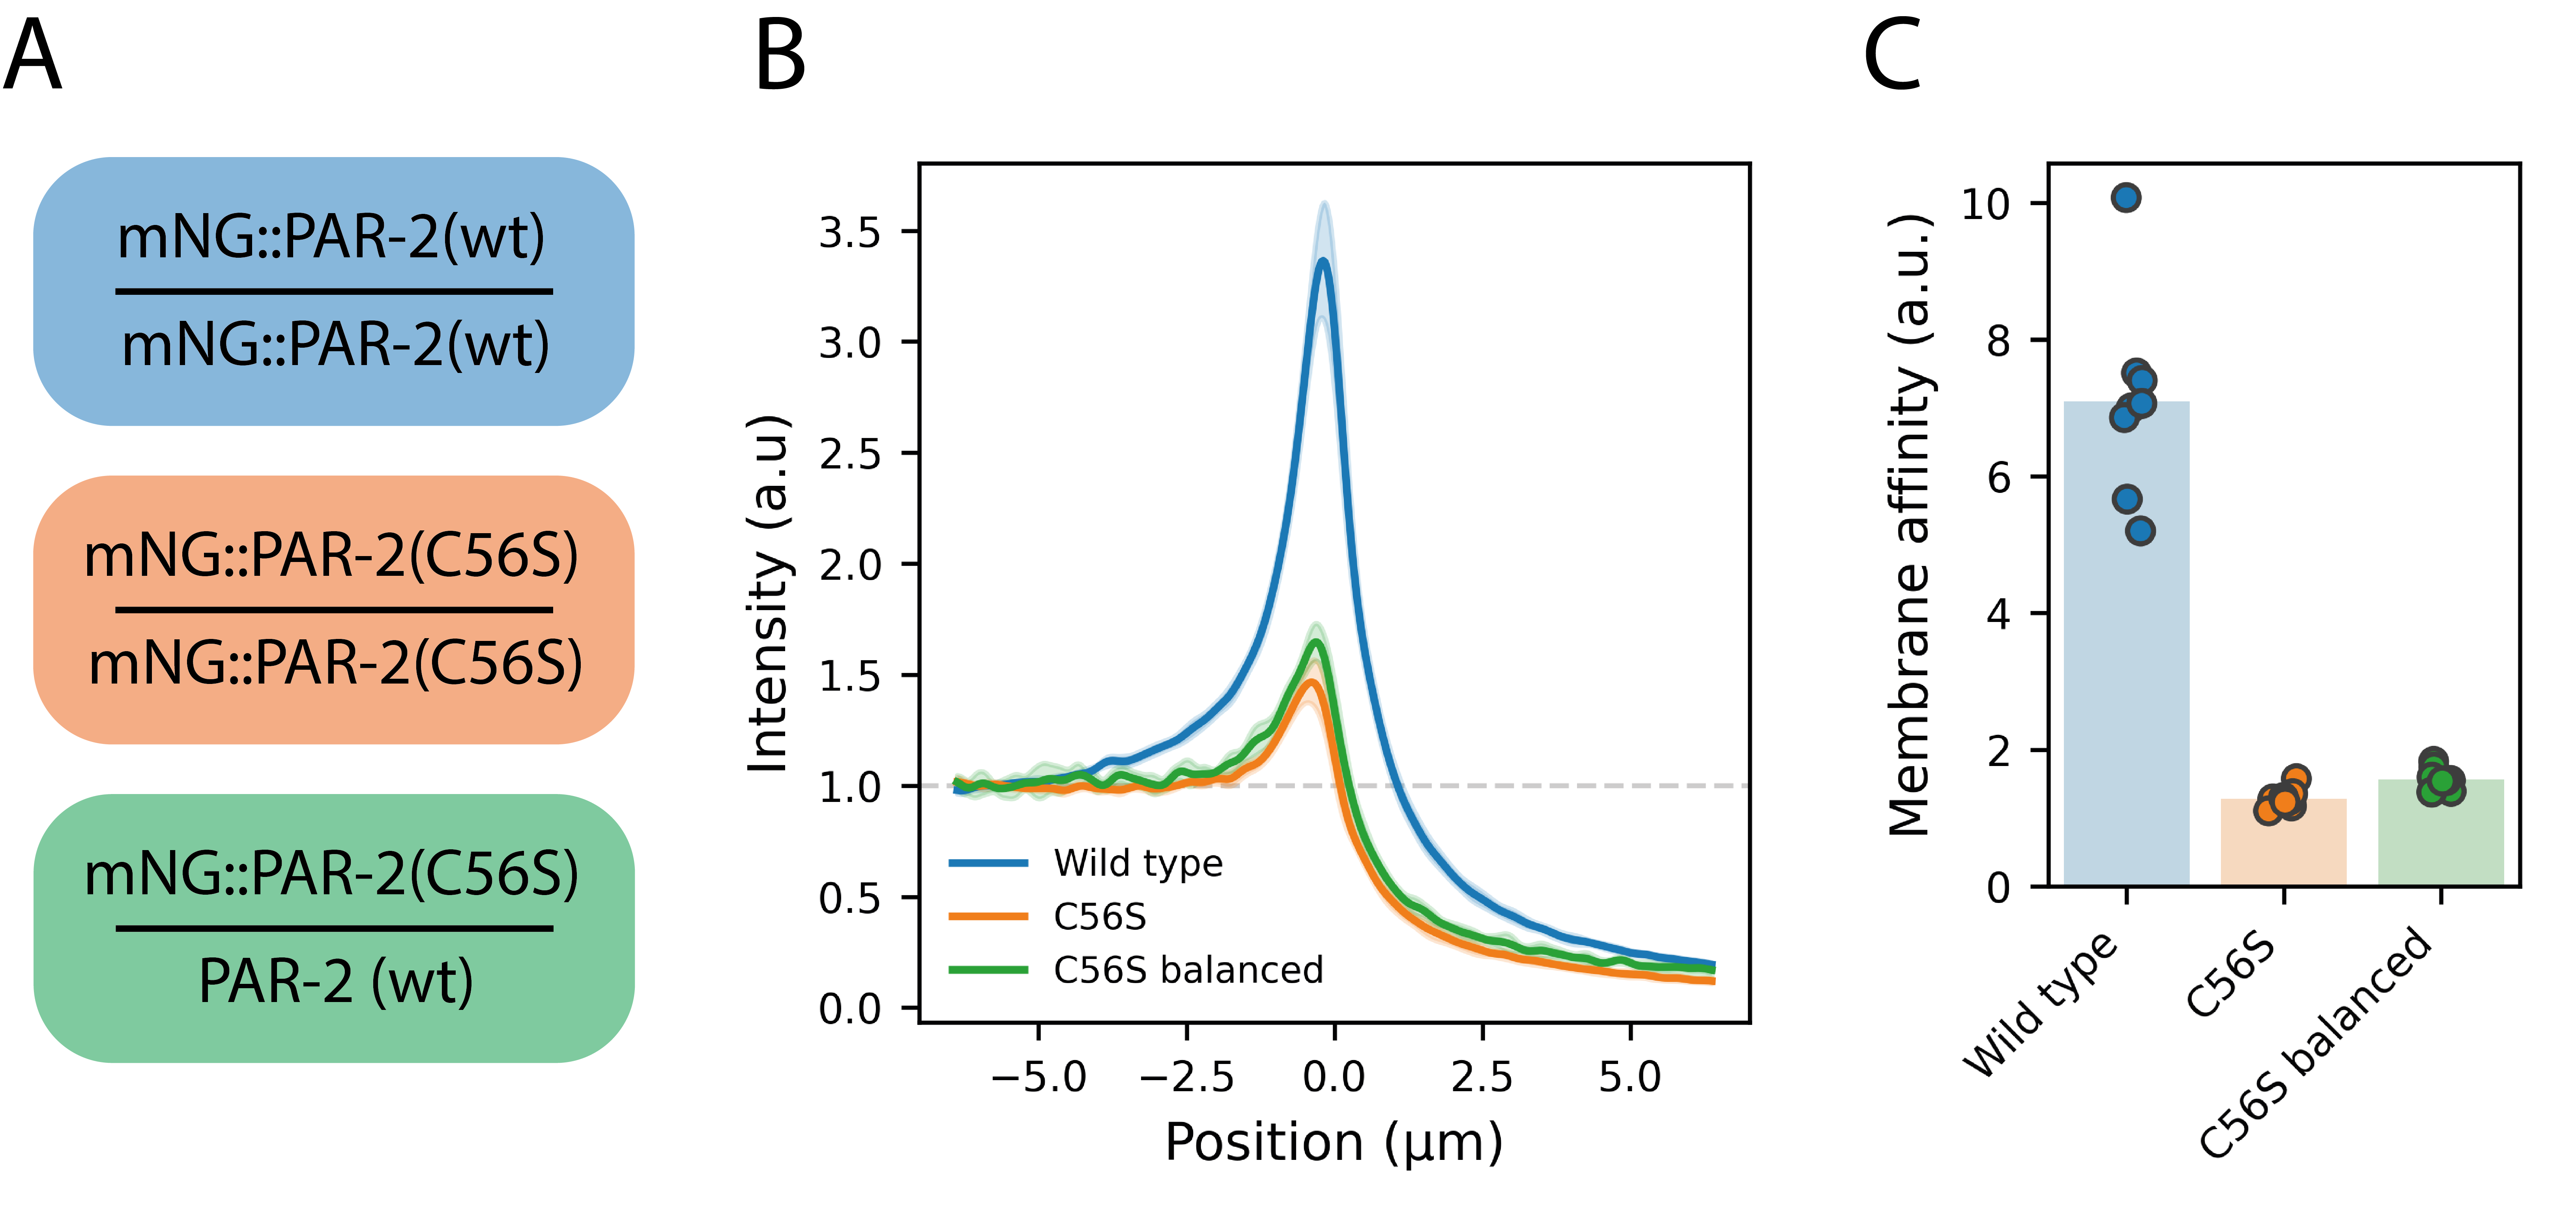
\includegraphics[scale=1]{c56s_cis}
\centering
\mycaption{The PAR-2 RING domain activity is cis-acting}{
\textbf{(A)} Schematic of the three genotypes investigated. Quantification results represent the distribution of mNG-tagged PAR-2 only.
\textbf{(B)} Normalised cross-cortex profiles averaged over the posterior domain for the three conditions. 
\textbf{(C)} Membrane affinity measurements for the three conditions, measured over the posterior domain of polarised cells.
}
\label{fig:c56s_cis}
\end{figure}

RING domains were originally described by \textcite{Freemont1991} as a commonly occurring motif, between 40 and 70 residues in length, with a characteristic pattern of cysteine and/or histidine residues. Structural studies have since revealed a ‘cross-brace’ pattern, whereby these cysteine and histidine residues interact with two zinc ions to form a characteristic folded structure (\cref{fig:ring_schematic}). RING domains are highly prevalent, with 300 RING domain containing genes in the human genome \citep{Li2008}. Two roles have been commonly attributed to RING domains in other proteins: ubiquitination and dimerisation. In this chapter, I investigate each of these in turn as potential mechanism in the context of PAR-2 membrane association.\\

\begin{SCfigure}
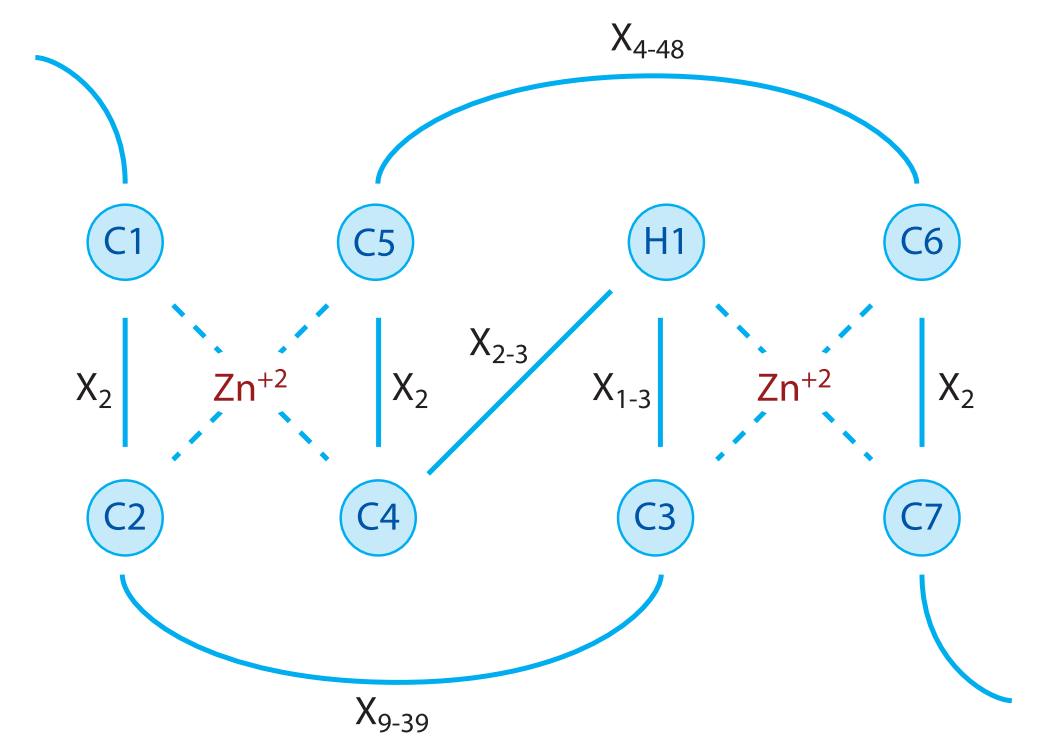
\includegraphics[scale=0.4]{ring_schematic}
\mycaption{Schematic of RING domain organisation}{
Cysteines interacting with zinc are labelled as C1 etc. H1 represents a zinc-interacting histidine. Xn refers to the number of amino acids in the spacer regions between the zinc ligands. Figure from \textcite{Deshaies2009}.
}
\label{fig:ring_schematic}
\end{SCfigure}


\section{Exploring a role for ubiquitination}

The most commonly associated role of RING domains is in the ubiquitination pathway, the mechanism by which ubiquitin (Ub) molecules are attached to substrate proteins. This pathway involves three classes of enzymes which catalyse three steps (\cref{fig:ubiquitination_pathway}): ubiquitin-activation (E1), ubiquitin-conjugation (E2), ubiquitin-ligation (E3), the latter of which is commonly attributed to RING domain proteins. E1 activates ubiquitin and transfers to an E2, where a thioester bond is formed between the E2 and Ub. E3s then simultaneously interact with a substrate and the E2-Ub conjugate to catalyse the transfer of Ub to a target lysine on the substrate. \\

\begin{figure}[!h]
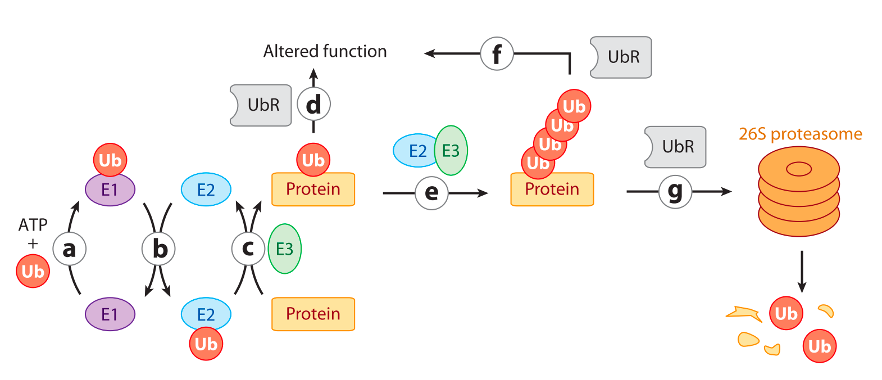
\includegraphics[scale=0.95]{ubiquitination_pathway}
\setlength{\abovecaptionskip}{20pt}
\centering
\mycaption{Schematic of the ubiquitination pathway}{Figure from \cite{Deshaies2009}}
\label{fig:ubiquitination_pathway}
\end{figure}

A single E1 works with several E2s ($\sim$ 40 in humans, 22 in \textit{C. elegans}), which work with hundreds of E3s. The choice of E2 often determines the type of ubiquitination that occurs. This can be either monoubiquitination, where a single ubiquitin molecule is added to a target lysine, or polyubiquitination, meaning the formation of a ubiquitin chain via lysine molecules on ubiquitin monomers. The functional consequences of ubiquitination are directly related to the type of ubiquitination that occurs. Monoubiquitination is associated with modification of protein function, and can regulate the structure of a protein, change it's binding partners or change it's cellular localisation. Depending on the type of linkage, polyubiquitination can also be associated with modification of protein function, but is most commonly associated with proteasome-dependent proteolysis. Each E3 typically interacts with only a small number of E2s, and a small number of substrates. Therefore, by acting as a bridge between a specific E2 and a specific substrate, E3s are responsible for conferring specificity to the ubiquitination reaction. \\

It is thought that most RING domain proteins possess E3 ligase activity \citep{Deshaies2009}, catalysing the transfer of Ub directly from an E2 to a target substrate. RING E3s work by binding to and stabilising the `closed' conformation of an E2-Ub conjugate. This alters the geometry of the thioester bond between Ub and E2, increasing reactivity towards a substrate lysine residue. At the same time as interacting with the E2, most RING E3s bind to a substrate, bringing a specific lysine on the substrate into close proximity of the E2. This then leads to direct transfer of Ub from the E2 to the substrate. Typically, this E3/substrate interaction is via other parts of the E3 protein, rather than the RING domain itself (e.g. the TRIM class of E3s use C-terminal substrate recognition domains).\\

Alternatively, lysines on the E3 protein itself can be targeted (autoubiquitination). In many cases this may be a side effect of E3 activity with no functional role, but in some cases this may serve a purpose. For example, autoubiquitination of BCA2 has been demonstrated as an elegant mechanism to regulate steady state levels of the protein \citep{Amemiya2008}. As autoubiquitination is competitive with substrate ubiquitination, the protein is able to regulate its own levels according to substrate availability.\\

Given the common role for RING domain proteins as ubiquitin ligases, this function has long been suspected for PAR-2, but definitive evidence for ubiquitin ligase activity by PAR-2 has so far not been demonstrated. However, compatible with a potential role, yeast two hybrid assays show that PAR-2 interacts moderately with several E2 enzymes \citep{Gudgen2004}. Given that autoubiquitination is common for E3s, and that ubiquitination can change the properties of a protein, it's plausible that the defects observed in C56S mutants may relate to a failure to autoubiquitinate. In this section I aim to test PAR-2 for ubiquitination activity, and investigate the potential role of this in vivo.\\

\subsection{PAR-2 does not show activity in in vitro ubiquitination assays}

\textit{Work in this section was performed with Colin Davis in Anne Schreiber's lab, and Diego Esposito in Katrin Rittinger's lab, both at the Crick}\\

My first aim was to test for the ability of PAR-2 to act as a ubiquitin ligase. Typically, this property can be assayed in vitro using purified samples of a protein of interest. To express and purify PAR-2 we used an insect cell system, which was chosen for its ability to express high levels of large, complex proteins. We expressed strep-tagged full-length PAR-2 in insect cells, lysed cells by sonication, and purified by strep pull-down followed by size exclusion chromatography (SEC) (see Methods). From the initial pull-down stage, we observed two prominant bands close to the expected mass of PAR-2. Due to their similar masess, we were unable to separate the two bands by size exclusion chromatography (\cref{fig:ubiquitin_assay}A). We tested both bands by mass spectrometry, which confirmed them both to be PAR-2. Interestingly, a single site (K351) was found to be ubiquitinated in the sample corresponding to the upper band, explaining the higher mass of this population on the gel compared to the expected mass of strep-tagged PAR-2 (75.24 kDa). No ubiquitinated sites were found in the sample corresponding to the lower band, which sits closer to the expected weight of PAR-2, although the K351 site was not covered by mass spectrometry results, so we cannot confirm that this site wasn't ubiquitinated. We also observed two similar bands in a small-scale prep of PAR-2 (C56S) (data not shown). Therefore, I do not believe this to be a result of autoubiquitination, but may rather represent ubiquitination of the protein by an insect ubiquitin ligase within the insect cells. CRISPR mutation of K351 to an alanine has no effect on PAR-2 localisation in vivo (data not shown), and previous attempts to purify PAR-2 from worm lysates and HEK cell preps have not shown two bands.\\

Sample from SEC purification was pooled (lanes 1-9) and used for an in vitro ubiquitination assay. Designed to test for ubiquitination activity of a protein, this assay involves mixing a text protein with ubiquitin, E1 and an E2, and observing for autoubiquitination of the test protein (see Methods). Given that E3s typically work with only a small number of E2s, the assay is sensitive to the choice of E2, and therefore care must be taken to choose an appropriate E2. In the case of PAR-2 this is so far unknown, although PAR-2 has been shown to weakly interact with UBC-2, UBC-18 and UEV-2 in yeast two hybrid assays \citep{Gudgen2004}. Since UBC-2 (known as UBCH5a in Humans) is also the most promiscuous of the E2s, this was chosen for the assay. As shown in \cref{fig:ubiquitin_assay}, whereas a positive control sample (TRIM2) showed rapid auto-polyubiquitination and depletion of the ubiquitin pool within 30 minutes, no effect was observed for PAR-2 across the whole 60 minutes of the experiment, indicating lack of detectable ubiquitination activity. A similar assay was performed using human UBC13/UEV1 as the E2, chosen based on PAR-2's sequence similarity to the E3 ligase RNF8, which works with this E2, however the result of this was also negative (data not shown).\\

\begin{figure}
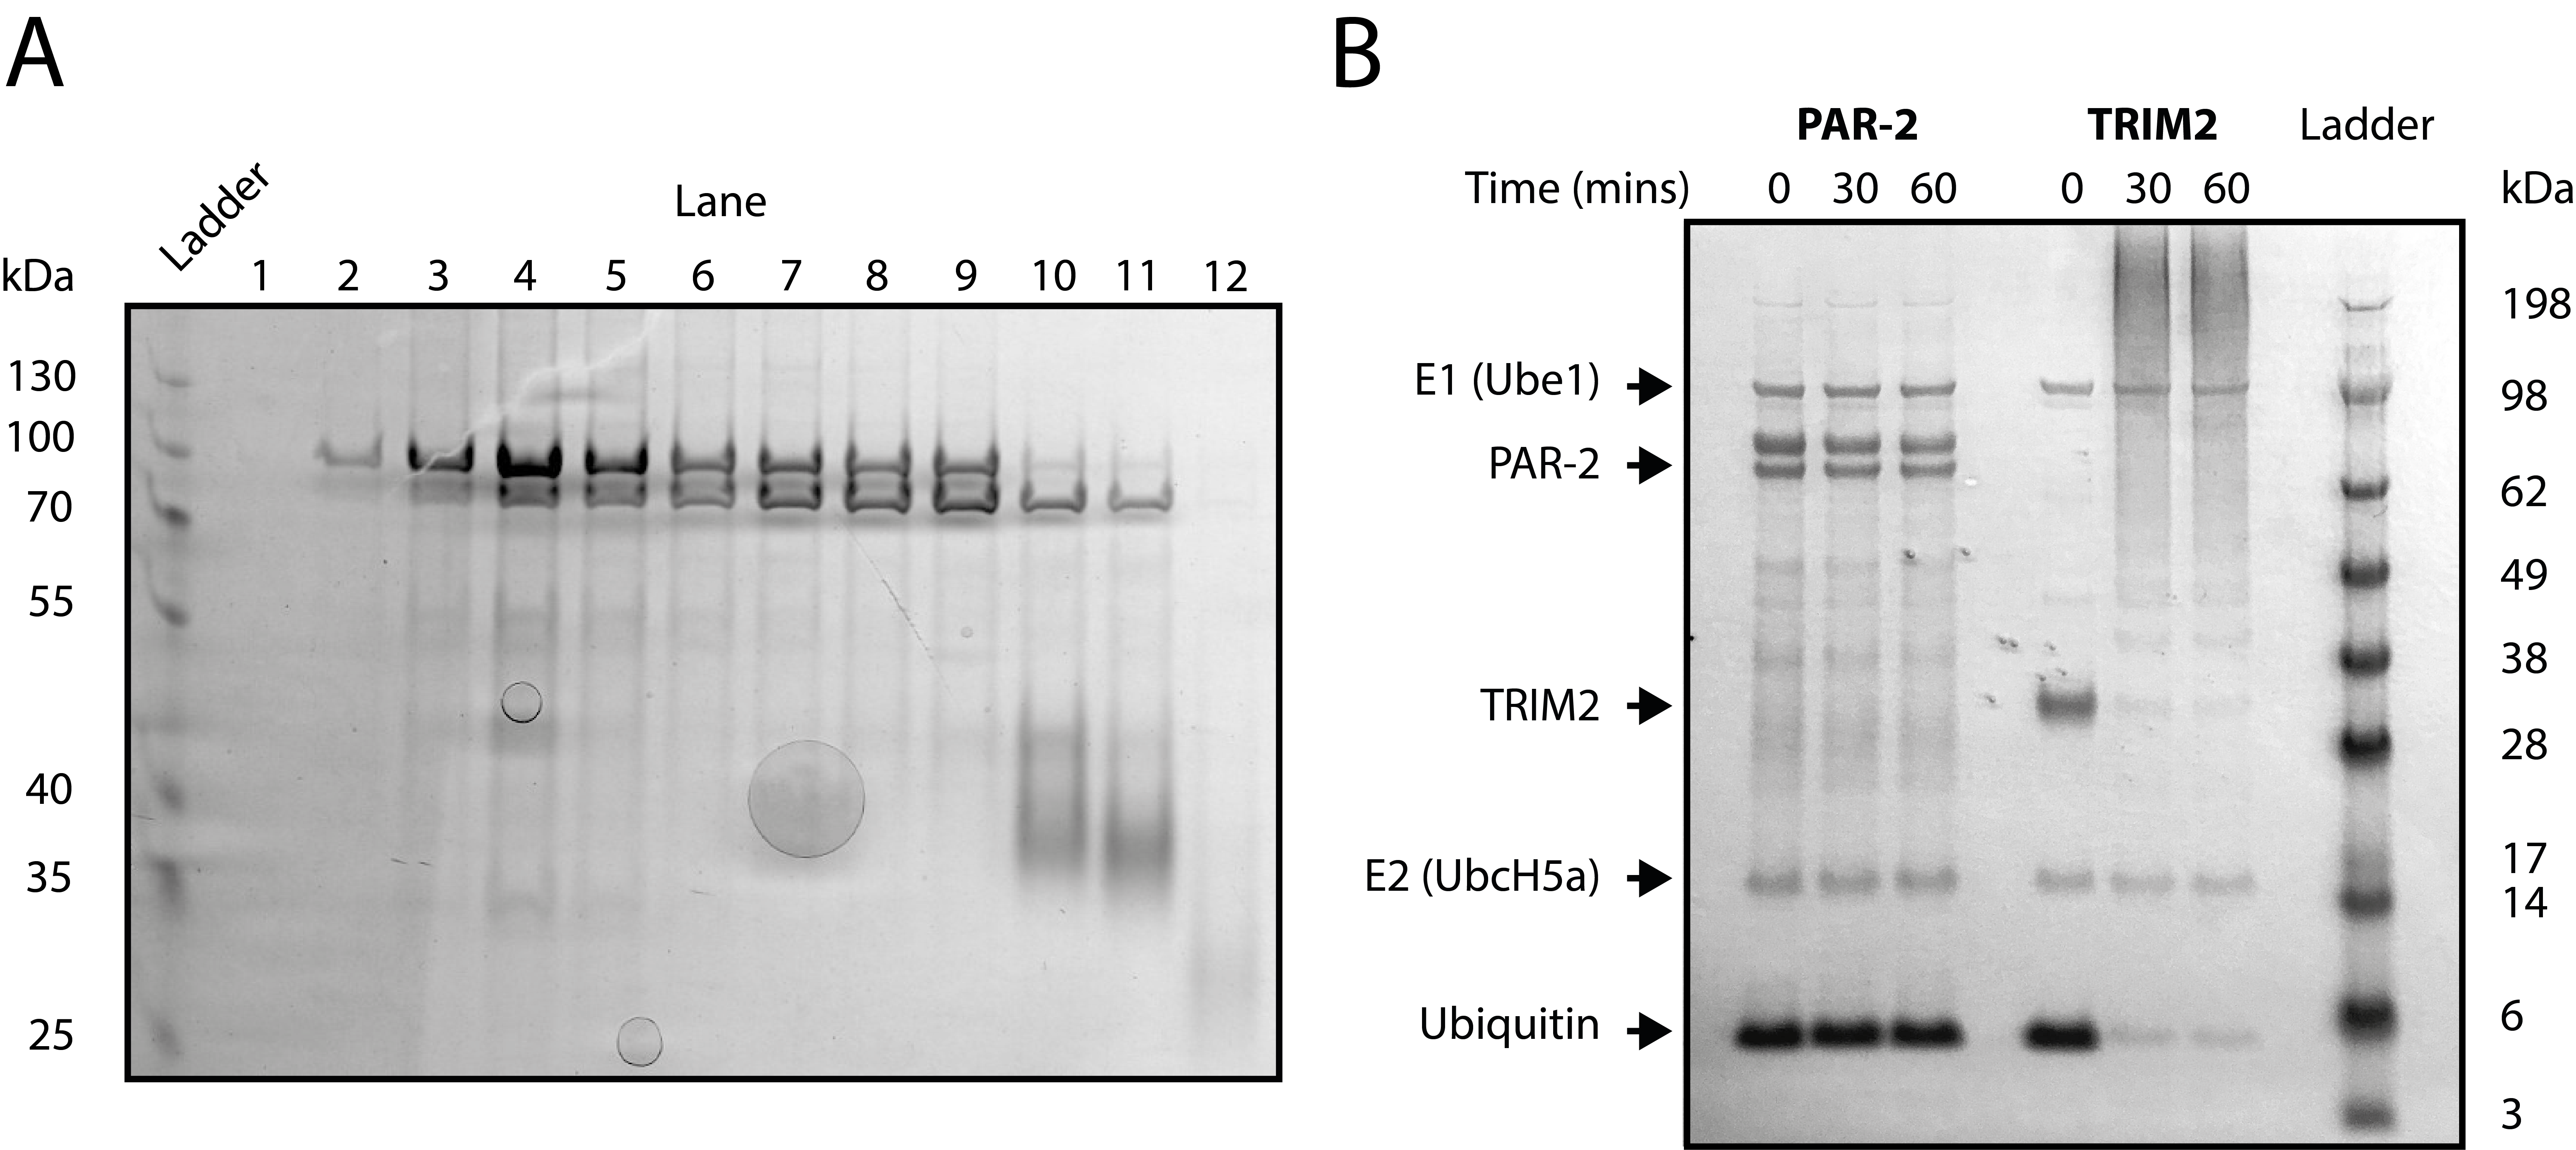
\includegraphics[scale=1]{ubiquitin_assay}
\centering
\mycaption{PAR-2 does not show activity in an in vitro ubiquitination assay}{
\textbf{(A)} Size exclusion chromatography results for a sample of strep-tagged PAR-2 purified from insect cells. The two prominent bands in the 70-100 kDa region both contain PAR-2. Expected weight (with strep tag) = 75.24 kDa.
\textbf{(B)} Ubiquitination assay results for PAR-2 vs TRIM2. Whereas TRIM2 displays auto-polyubiquitination activity, as shown by the appearance of 'streak' at high masses representing polyubiquitinated protein, loss of unmodified TRIM2 and loss of free ubiquitin, no activity is observed for PAR-2 throughout the entire assay. 
}
\label{fig:ubiquitin_assay}
\end{figure}


\subsection{Targeted mutation to putative linchpin site has no phenotype}

Whilst C56S mutation has a clear and strong effect in vivo, this does not necessarily imply a role for PAR-2 as a ubiquitin ligase, as unfolding the domain may have a multitude of effects. Therefore, to test the potential role of ubiquitination in vivo, I aimed to specifically disrupt E3 ligase activity without disrupting the core structure of the RING domain.\\

Whilst mechanisms of catalytic activity are variable among proteins, a key catalytic site found in many RING E3 ligases is an arginine or lysine residue immediately downstream of the final zinc-coordinating cysteine, known as the linchpin site, which forms a hydrogen bond with the E2 to stabilise the closed (active) state \citep{Pruneda2012}. Mutation of this site to an alanine has been shown, for several proteins, to abrogate RING domain catalytic activity \citep{Pruneda2012}. Typically, the choice of residue at this site regulates a trade-off between ubiquitination activity and E2 specificity. RINGs with a K at this site typically show lower ubiquitination activity in vitro but higher E2 specificity. \textcite{Stewart2017} showed for the protein BRCA1 that mutating this site from an arginine to a lysine increases ubiquitination activity but reduces E2 specificity. 46\% of RING domains have an arginine at this site linchpin, whereas 14\% have lysine \citep{Stewart2017}. However, many known RING E3 ligases have neither an arginine or lysine at this site (such as several members of the TRIM family of RING E3 ligases, \cref{fig:linchpin_alignments}B), suggesting that other mechanisms of E2 activation must exist. Currently this is poorly understood.\\

\textit{C. elegans} PAR-2 has a lysine at the canonical linchpin site, which suggests that the standard linchpin mechanism for E2 activation could apply. Alignment of \textit{Caenorhabditis} PAR-2 RING domain sequences shows that this site is largely conserved as a lysine across the genus (\cref{fig:linchpin_alignments}A), but \textit{C. bovis}, \textit{C. castelli} and \textit{C. monodelphis} have neither an arginine nor a lysine at this site. The fact that this site isn't universally conserved may argue against an important role for ubiquitination activity, could suggest that PAR-2 does play an role as a ubiquitin ligase but doesn't rely on the linchpin mechanism, or could suggest that these other species have evolved alternative strategies distinct from \textit{C. elegans}.\\ 

\begin{figure}
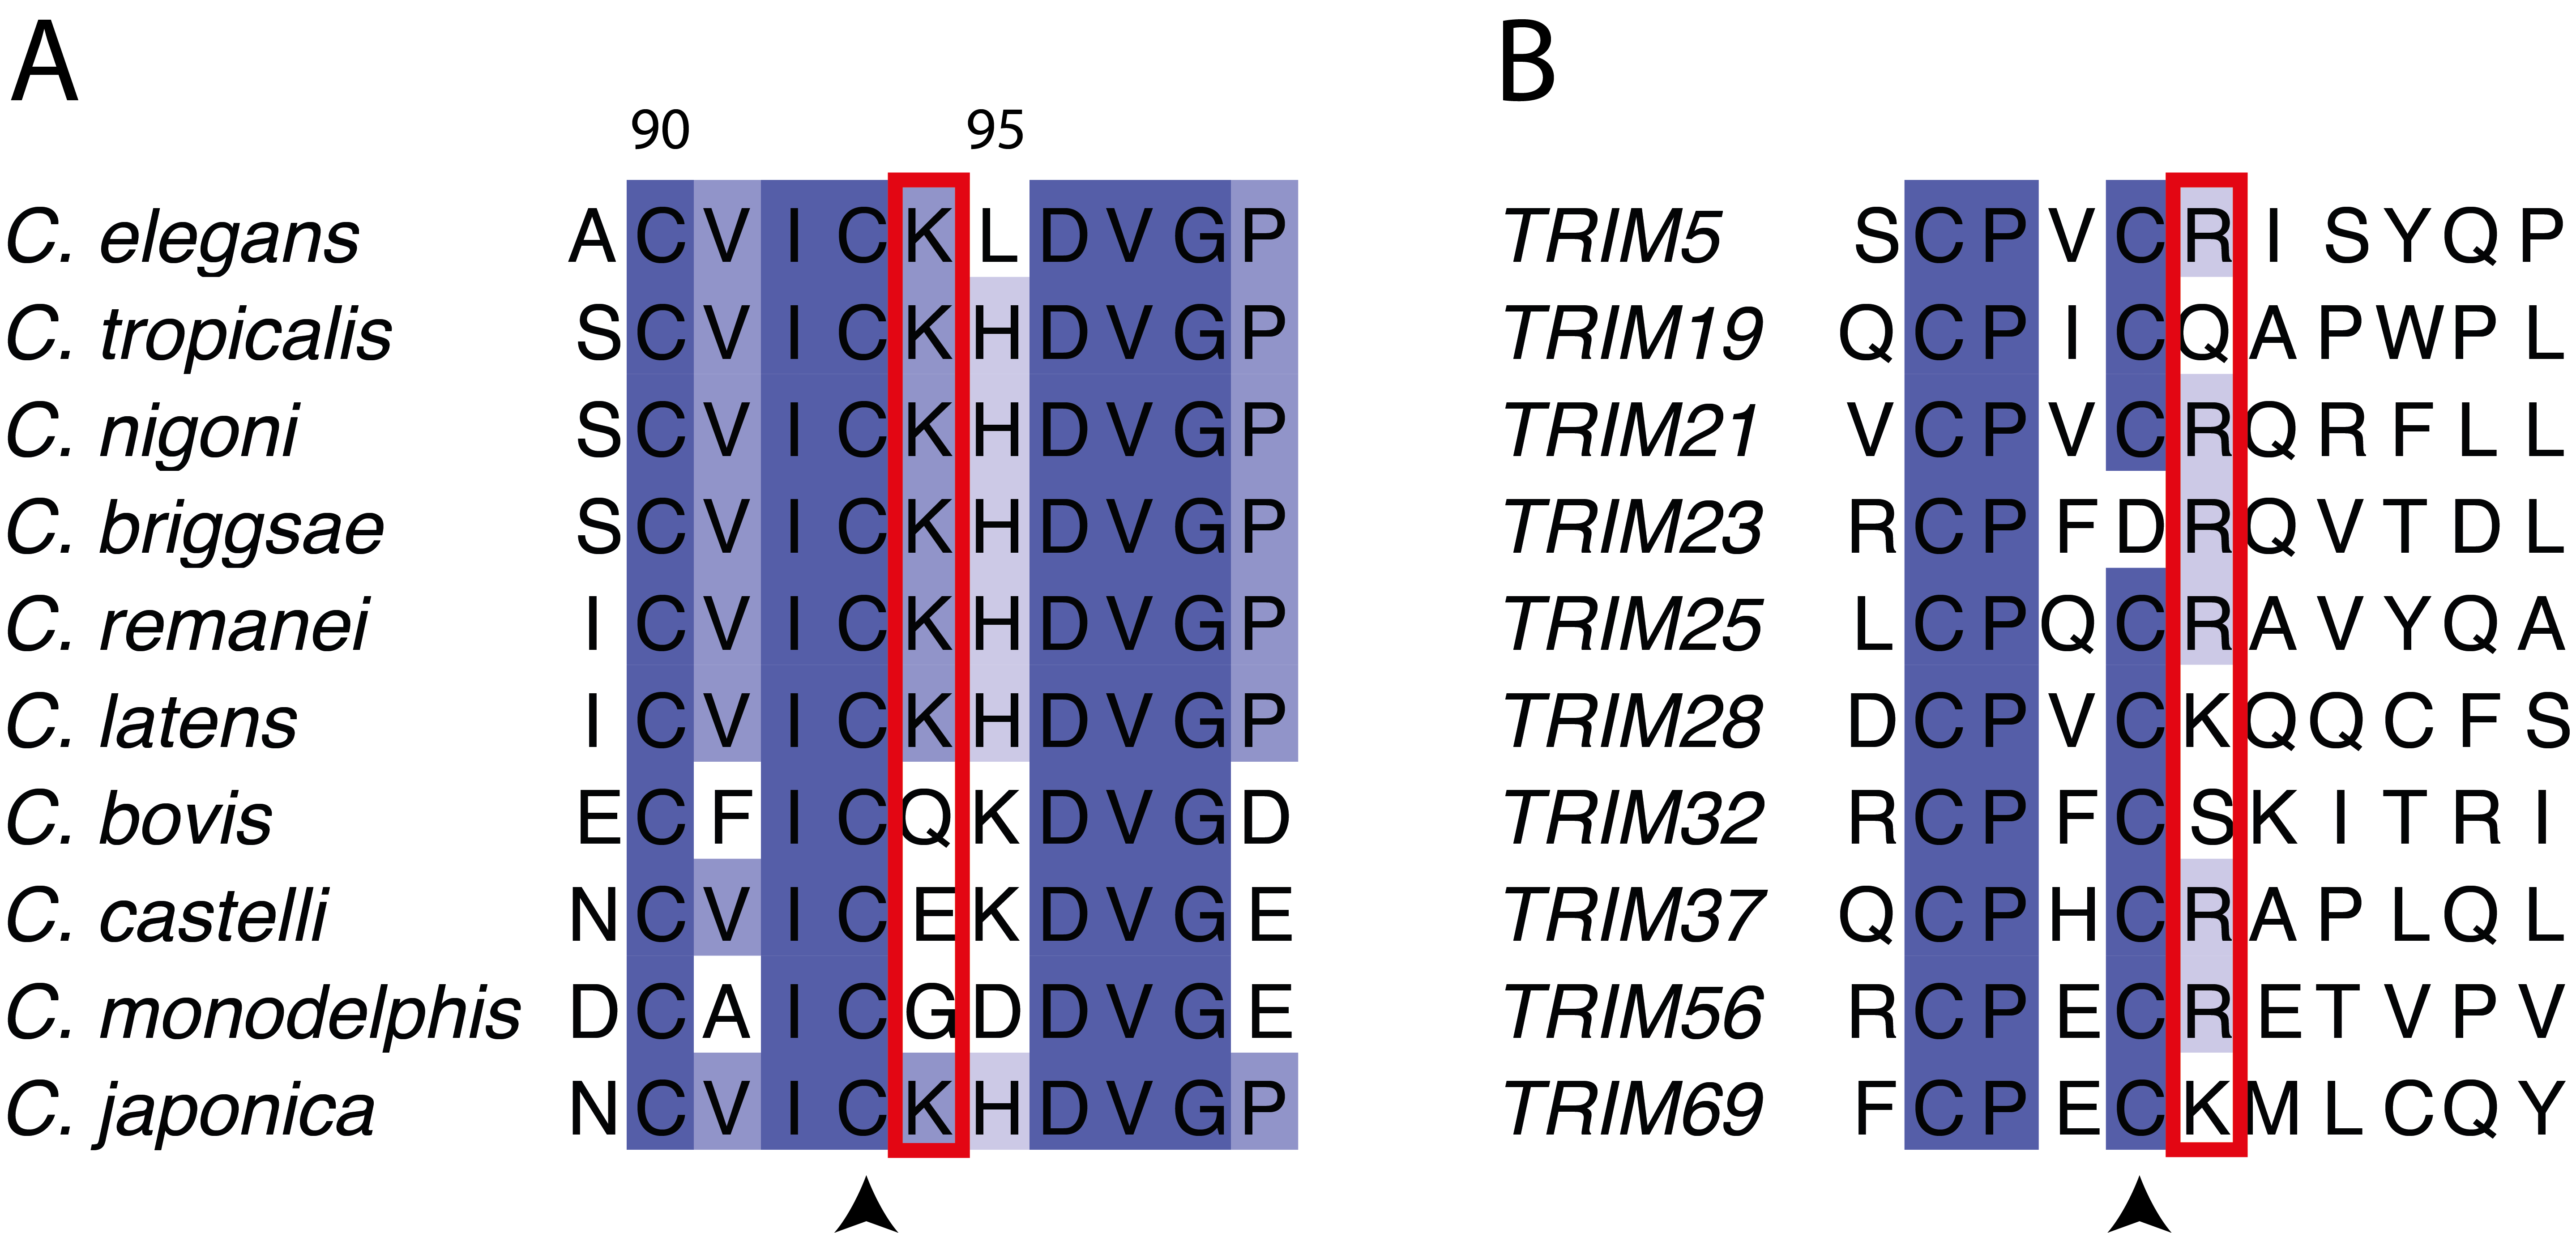
\includegraphics[scale=0.9]{linchpin_alignments}
\centering
\mycaption{Linchpin site alignments}{
\textbf{(A)} Alignment for the PAR-2 linchpin site (red box) across species of the \textit{Caenorhabditis} genus. This site is largely conserved as a lysine, but some species do not follow this pattern.
\textbf{(B)} Alignment of the linchpin site across the TRIM family of ubiquitin ligase proteins. In most cases this is an arginine or a lysine, but in some cases a different amino acid is present.
}
\label{fig:linchpin_alignments}
\end{figure}

To test the potential role of linchpin-mediated autoubiquitination for PAR-2 membrane binding affinity, I used CRISPR to perform targeted mutation to this site, turning it into an alanine. As shown in \cref{fig:linchpin_in_vivo}, this has no detectable effect on membrane affinity. Whilst this cannot rule out a role for PAR-2 as a ubiquitin ligase in vivo, the result argues against a model in which linchpin-mediated autoubiquitination is a driver of high membrane association.\\

\begin{figure}
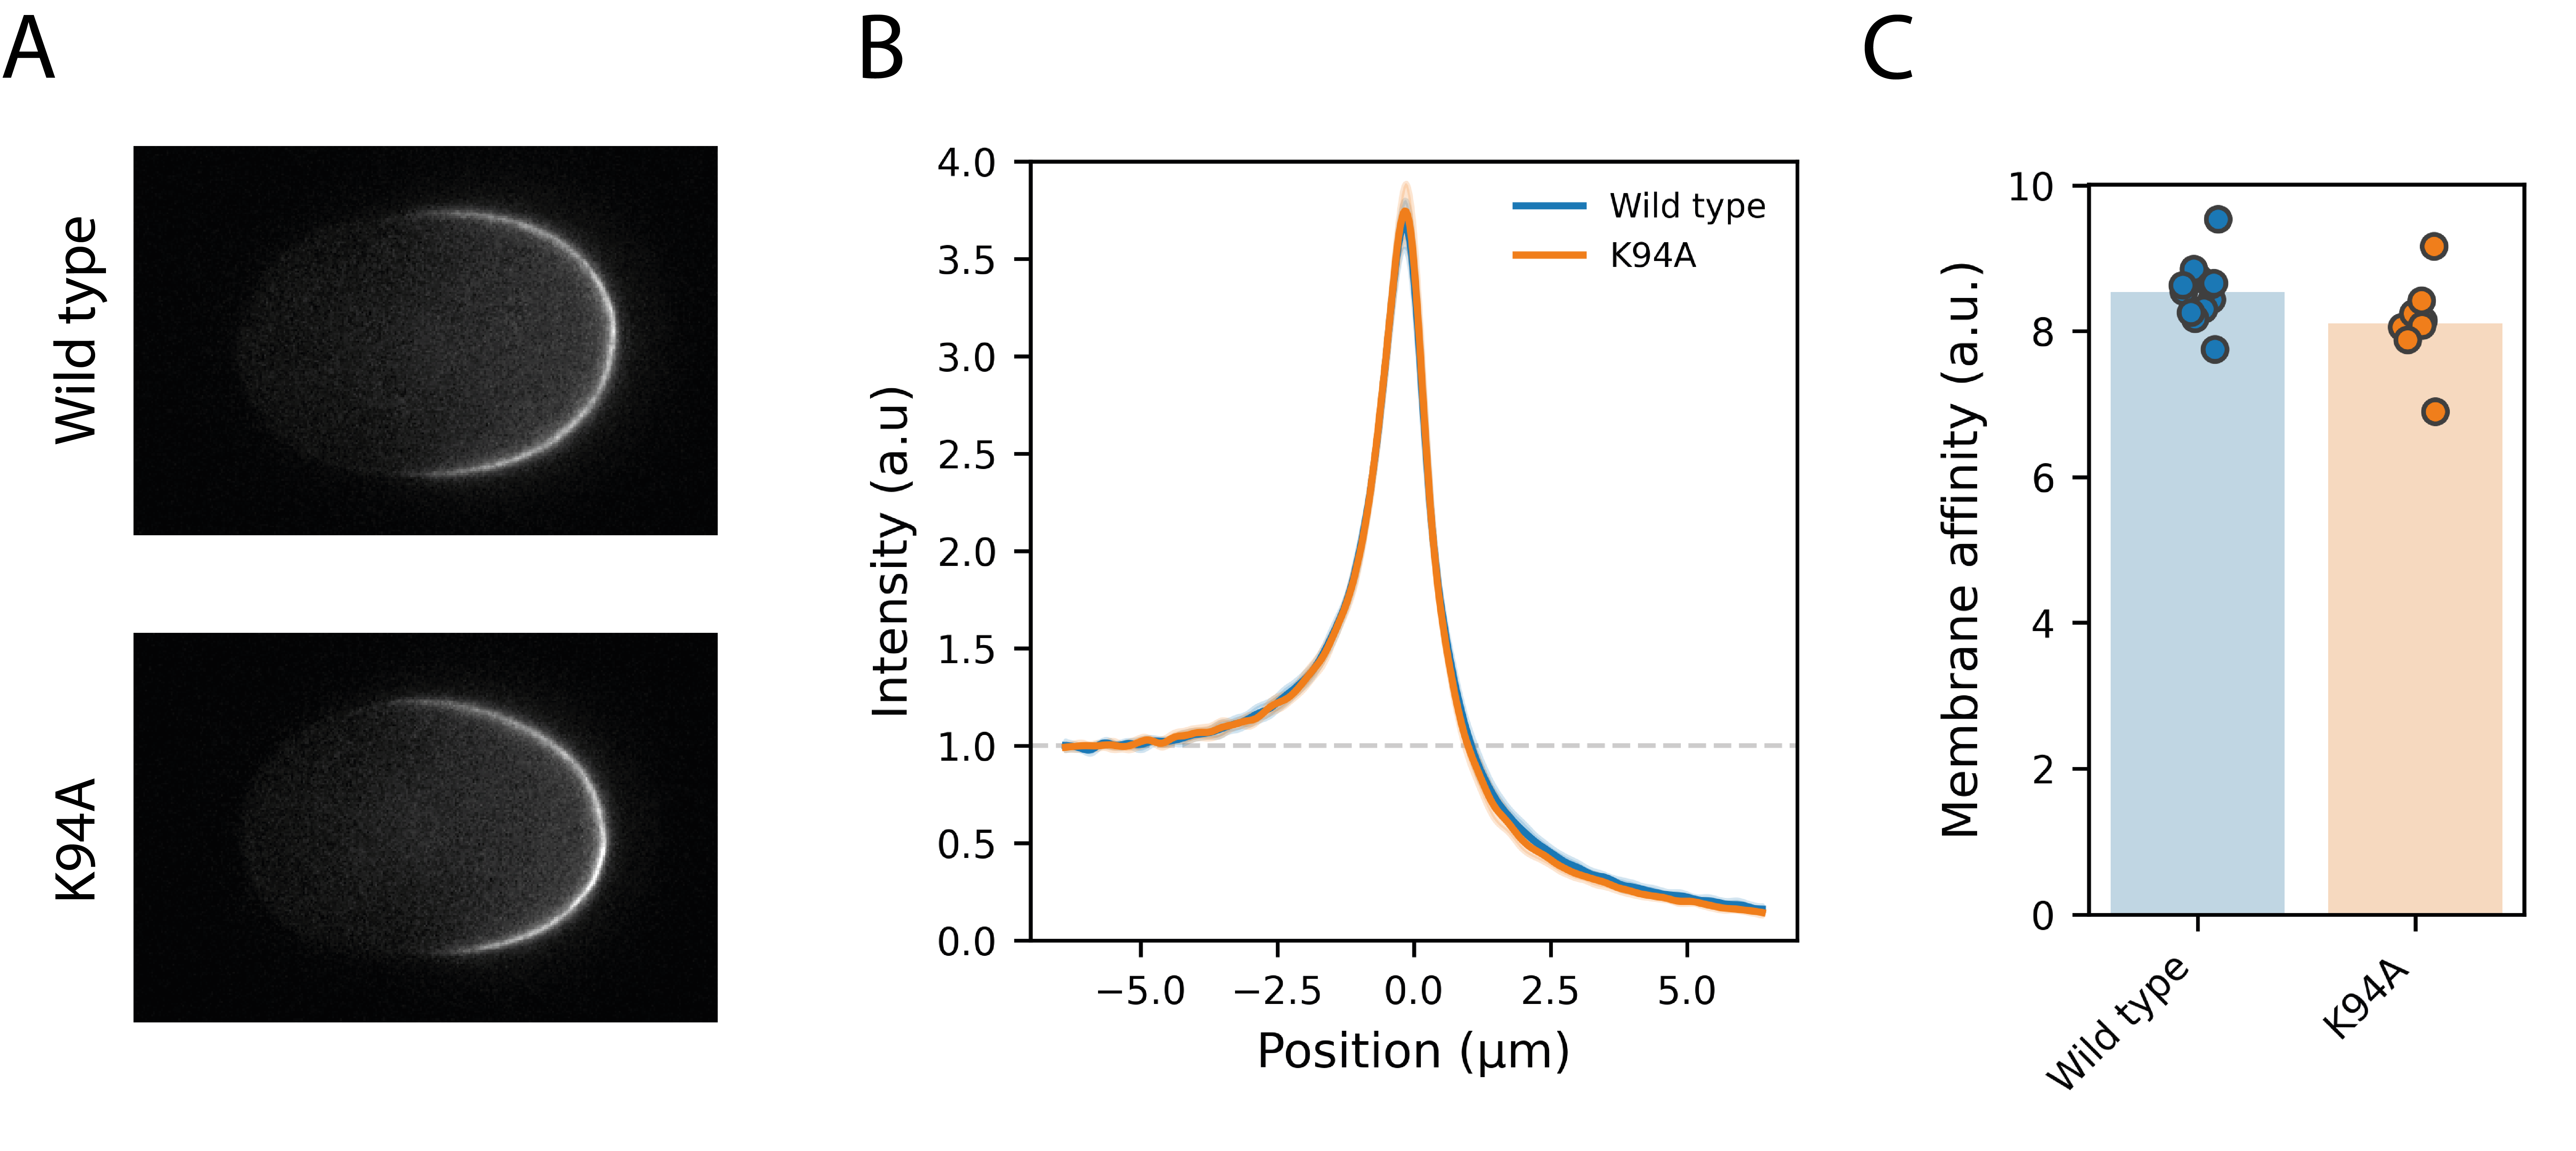
\includegraphics[scale=0.9]{linchpin_in_vivo}
\centering
\mycaption{Mutation of the PAR-2 linchpin site has no effect on membrane affinity}{
\textbf{(A)} Midplane images of wild type vs K94A GFP::PAR-2 at maintenance phase.
\textbf{(B)} Normalised cross-cortex profiles for wild type vs K94A PAR-2 averaged over the posterior domain.
\textbf{(C)} Membrane affinity measurements for wild type vs K94A PAR-2 in the posterior domain.
}
\label{fig:linchpin_in_vivo}
\end{figure}


\subsection{Discussion}

Whilst the results in this section do not provide evidence to support PAR-2 ubiquitin ligase activity, it's difficult to draw strong conclusions. Negative results in the ubiquitination assay could indicate lack of E3 ligase activity, but may have  also been caused by an inappropriate E2, damage to the protein during purification, or there could be a low level of activity that's below the detection threshold of the assay. The first point could be addressed by using an E2 scan, an approach that tests for activity using a wide array of available E2s, but this hasn't yet been explored. Negative results for the linchpin mutant could argue that PAR-2 doesn't act as an E3 ligase (at least not in a way that would impact membrane affinity), but given that the linchpin mechanism isn't universally conserved in E3s, ubiquitination activity cannot be ruled out.\\

% other possible ways of disrupting E2 interaction?

\clearpage
\section{Exploring a role for dimerisation}

Another key function attributed to RING domains is their ability to act as dimerisation domains. Many purified RING domains have been shown to self-associate in crystal structures, forming dimers or higher order oligomers. In most cases, dimerisation is achieved via hydrophobic interactions between short alpha-helical segments N and C terminal of the core RING domain (N helix and C helix), which form a four-helix bundle, as well as additional hydrophobic contacts in the core RING domain (\cref{fig:trim25}). \\


\begin{SCfigure}
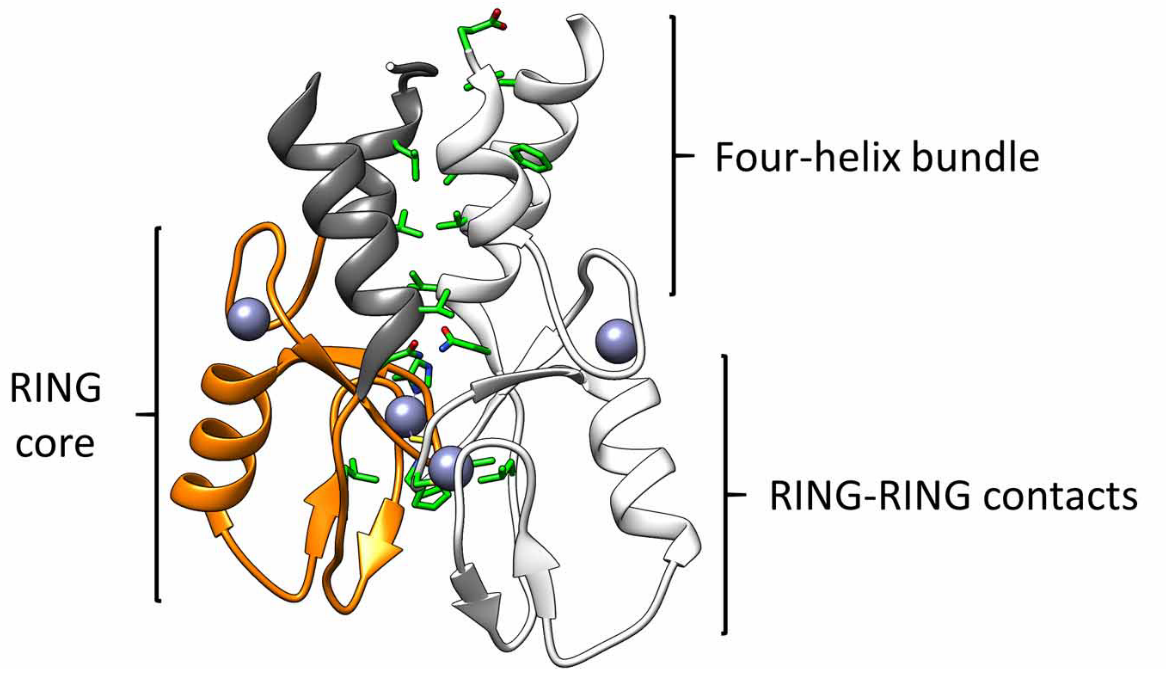
\includegraphics[scale=0.4]{trim25}
\mycaption{Structure of the TRIM25 RING domain dimer}{
A RING domain consisting of a zinc-interacting core (orange) flanked by N and C helices (dark gray) interacts with a second RING domain (white) to form a dimer. The dimer interface is characterised by a four-helix bundle and additional contacts between the RING cores. Hydrophobic residues at the interface are highlighted in green. Figure from \textcite{Fiorentini2020}.
}
\label{fig:trim25}
\end{SCfigure}

In many cases, the significance of dimerisation is fundamentally linked to the  role of RING-domain proteins as ubiquitin ligases. RING dimerisation helps stabilise the closed E2-Ub conformation, by allowing each Ub to make simultaneous contacts with two RING domains, which in many cases is essential for ubiquitination activity. Mutations to key hydrophobic residues in N and C helices have been shown to disrupt dimerisation and reduce ubiquitination activity for many RING domains \citep{Koliopoulos2016, Rojas-Fernandez2014, Liew2010}. On the other hand, forced dimerisation of RINGs can hyperactivate ubiquitination activity, as has been shown for RNF4 \citep{Rojas-Fernandez2014}. Given the widespread roles of protein dimerisation \citep{Goodsell2000}, it's also not unlikely that RING domains have evolved functions as dimerisation domains in other contexts unrelated to ubiquitination, however to the best of my knowledge this hasn't been explored.\\

Whilst the majority of RING domains are dimeric in crystal structures, their oligomeric state in solution varies dramatically, ranging from entirely monomeric to constitutively dimeric. For example, whereas TRIM32 appears constitutively dimeric in solution \citep{Koliopoulos2016}, TRIM21 exists in a monomer-dimer equilibrium \citep{Dickson2018}, and TRIM25, whilst crystalising as a dimer, appears entirely monomeric in solution, only dimerising at very high concentrations \citep{Koliopoulos2016}. \\

% comment on this, related to interface size?, deltaG? 

In the case of RING domains at the weaker end of the dimerisation scale, which exist largely as monomers in isolation, the ability to dimerise may be context specific. RNF4 is largely monomeric at physiological concentrations in vitro, but is able to dimerise upon addition of its substrate. Dual binding of two RNF4 molecules to a single substrate molecule creates a locally high concentration of RNF4 that permits dimerisation \citep{Rojas-Fernandez2014}. Similarly, TRIM25 shows weak dimerisation ability on its own, but dimerisation is stabilised by binding to an E2. \\

Notably, however, not all RING domains are dimeric.  Some form higher order structures (e.g. the TRIM19 RING, which forms a ‘torus-shaped’ tetramer in crystal structures), whereas others lack any ability to oligomerise. The TRIM28 RING domain, for example, has a small N helix, but lacks a C helix, and forms no dimerisation contacts in crystal structures \citep{Stevens2019}. The TRIM56 RING domain lacks both helices, and similarly is monomeric in crystal structures \citep{Fiskin2017}.\\

% Likewise, the CBL class of RING domains <more>..

In the case of PAR-2, the potential role for the RING domain as a dimerisation domain hasn't been tested, however full-length PAR-2 has been suggested to oligomerise. In vitro pull downs (\cite{Motegi2011}, \cite{Arata2016}) show that PAR-2 can weakly self-associate. \textcite{Arata2016} further showed by TIRF imaging that cortical PAR-2 exists as particles of varying size, which may represent a mix of monomers, dimers and possibly larger oligomers. In this section, I aim to test the dimerisation properties of the PAR-2 RING domain, and investigate the potential importance of this in vivo.\\

\subsection{PAR-2 RING domain sequence bears hallmarks of dimeric RINGs}

To investigate the potential role of the PAR-2 RING as a dimerisation domain, I began by analysing the sequence of the domain. I performed a BLAST search to compare the PAR-2 sequence against sequences of proteins for which the quaternary structure has been solved using laboratory methods, using the online SWISS model tool. This showed that the PAR-2 RING has sequence similarity to a number of well-characterised RING domains, most of which are dimeric in their crystal structures (\cref{tab:rings_pdb}). Sequence alignment shows that the PAR-2 sequence displays the general pattern of hydrophobic residues expected at the N and C helices of dimeric RING domains (\cref{fig:alignments_other_rings}).\\

\begin{table}[]
\centering
\begin{tabular}{|l|l|l|}
\hline
\textbf{Protein} & \textbf{PDB code} & \textbf{Quaternary structure} \\ \hline
TRIM69 & 6YXE & Dimer \\ \hline
RAD18 & 2Y43 & Dimer \\ \hline
RNF8 & 4AYC & Tetramer \\ \hline
TRIM21 & 6FGA & Dimer \\ \hline
TRIM25 & 5EYA & Dimer \\ \hline
TRIM5 & 4TKP & Monomer \\ \hline
\end{tabular}
\mycaption{RING domain proteins in the Protein Data Bank (PDB) with closest homology to the PAR-2 RING domain}{}
\label{tab:rings_pdb}
\end{table}

\begin{figure}
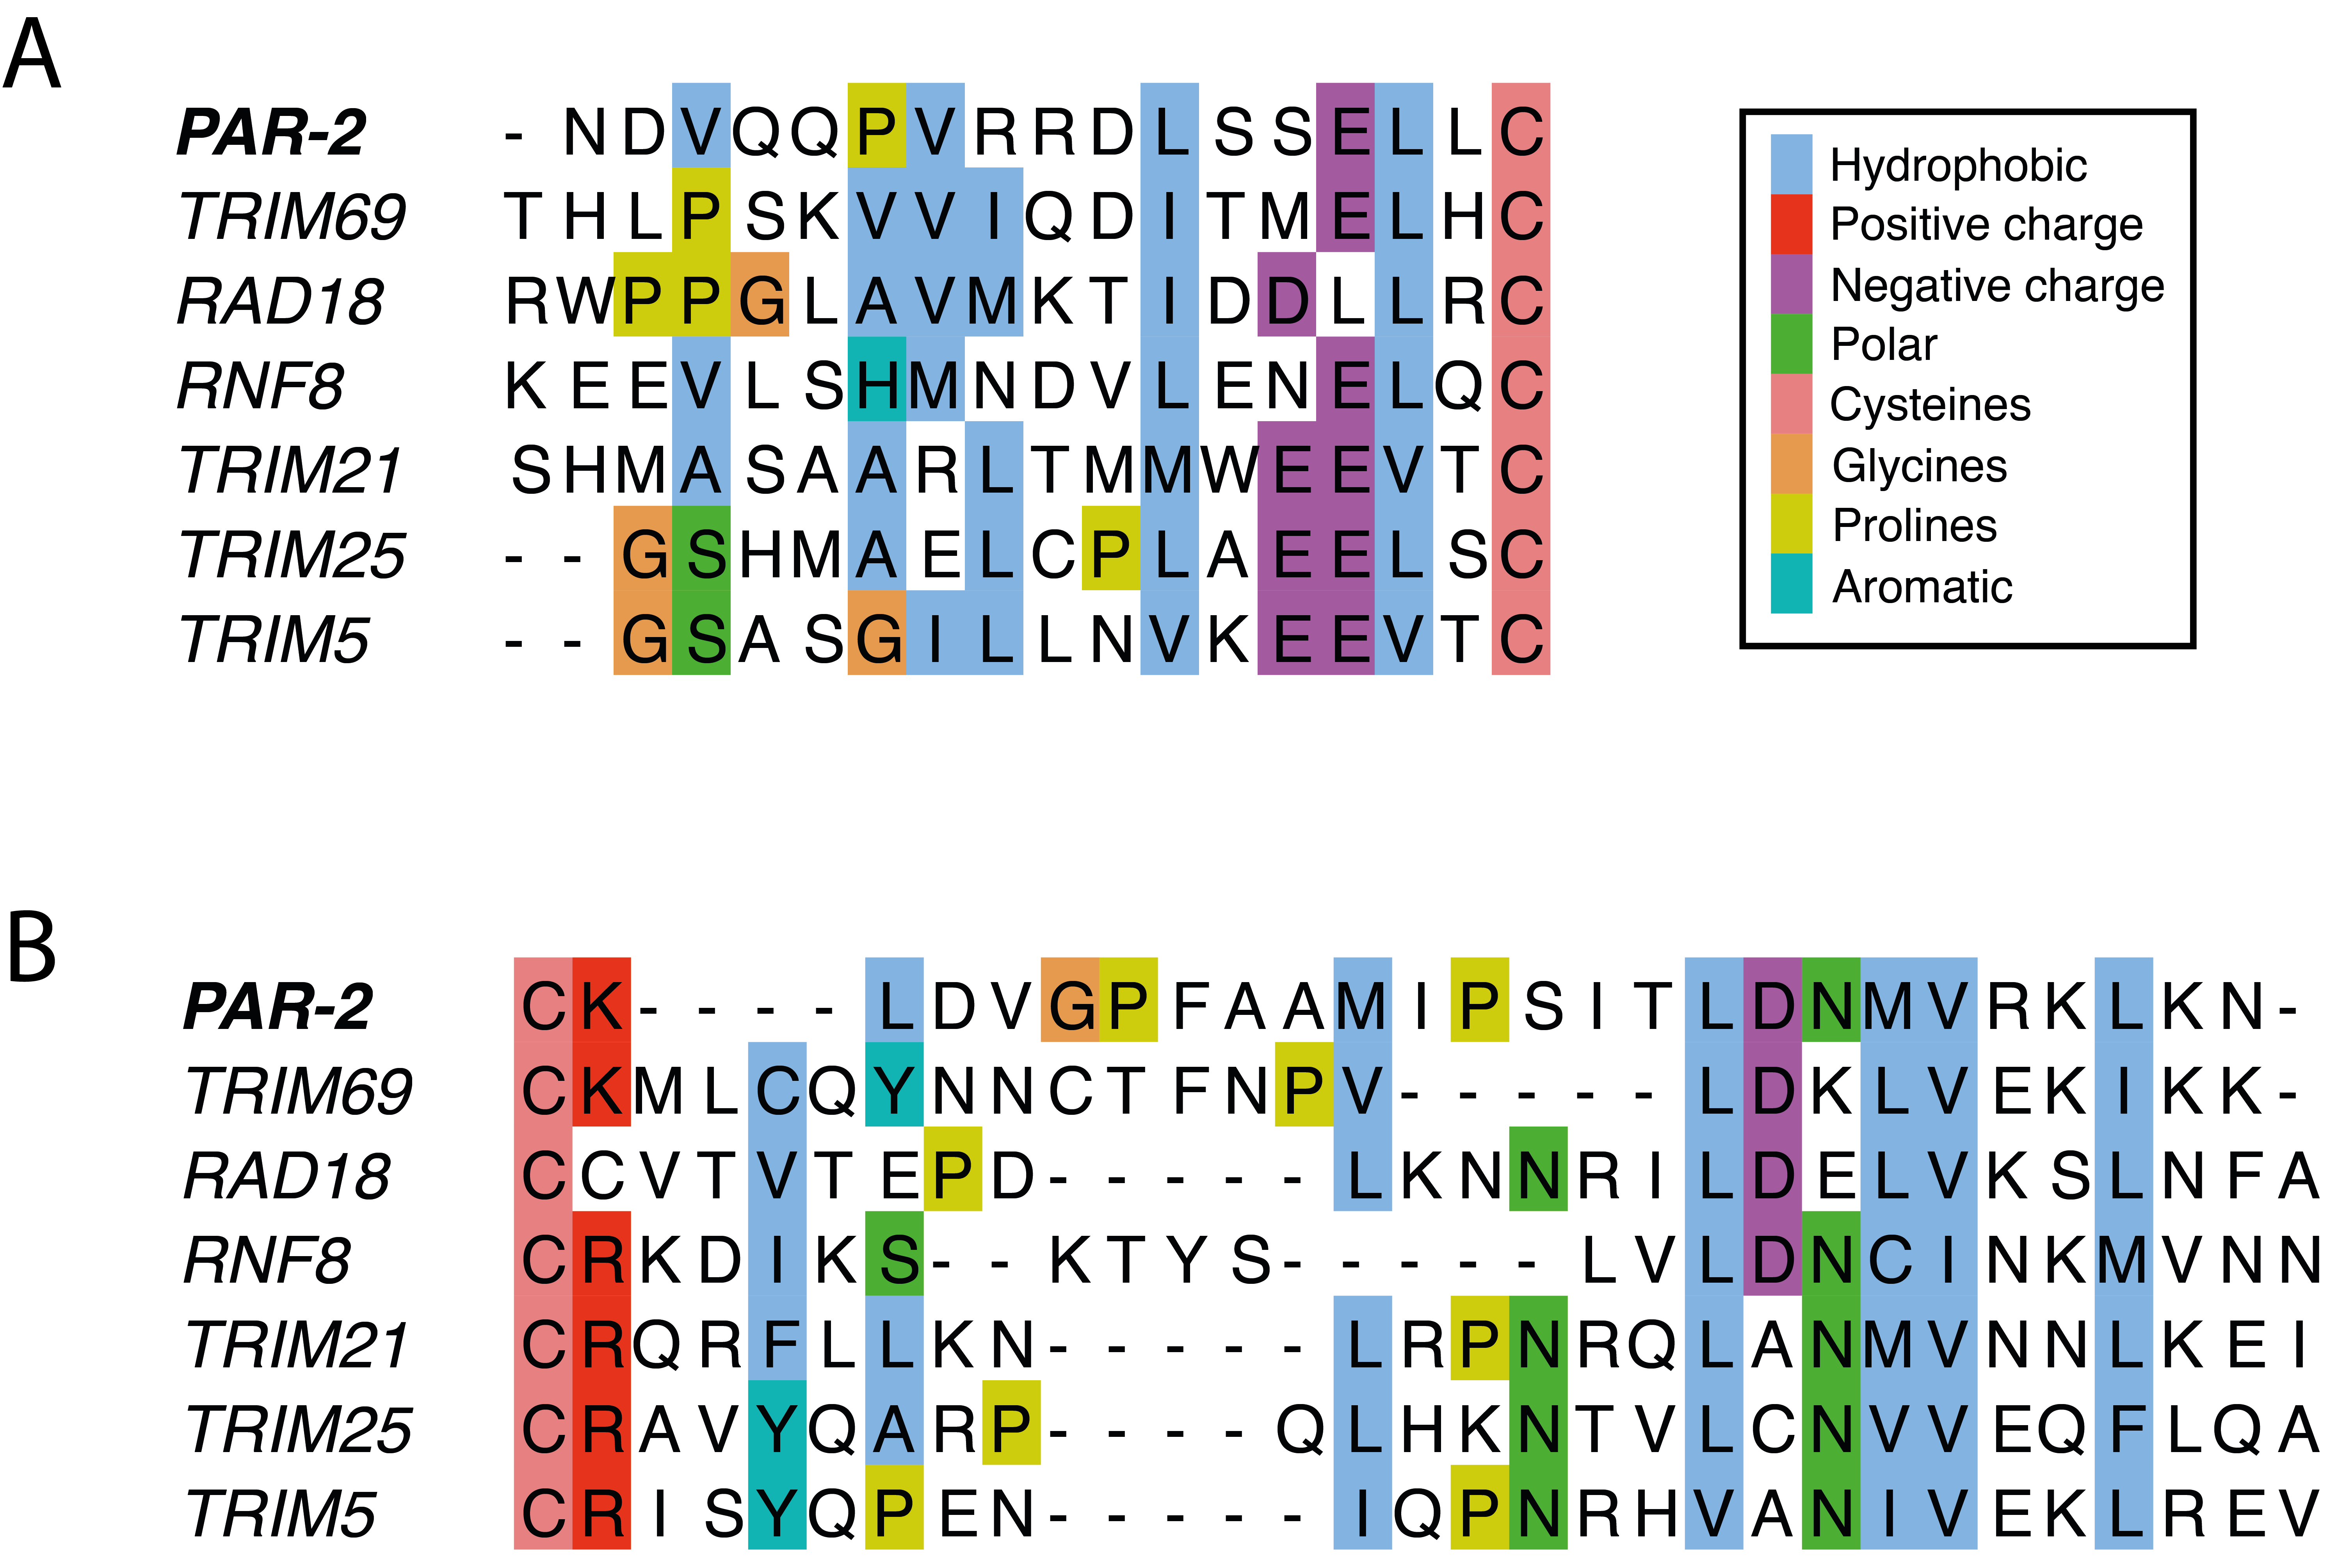
\includegraphics[scale=1]{alignments_other_rings}
\centering
\mycaption{Alignment of the PAR-2 RING domain N and C helices against similar proteins in the PDB}{
\textbf{(A)} N-helix alignment. Arrowhead indicates first zinc-coordinating cysteine of the core RING domain.
\textbf{(B)} C-helix alignment. Arrowhead indicates final zinc-coordinating cysteine of the core RING domain.
}
\label{fig:alignments_other_rings}
\end{figure}

These regions are also highly conserved in different \textit{Caenorhabditis} species (\cref{fig:alignments_par2}). Whilst there is some sequence variation, almost all species have an identical pattern of hydrophobic residues, which points to a potentially important role for PAR-2 RING domain dimerisation. \\

\begin{figure}
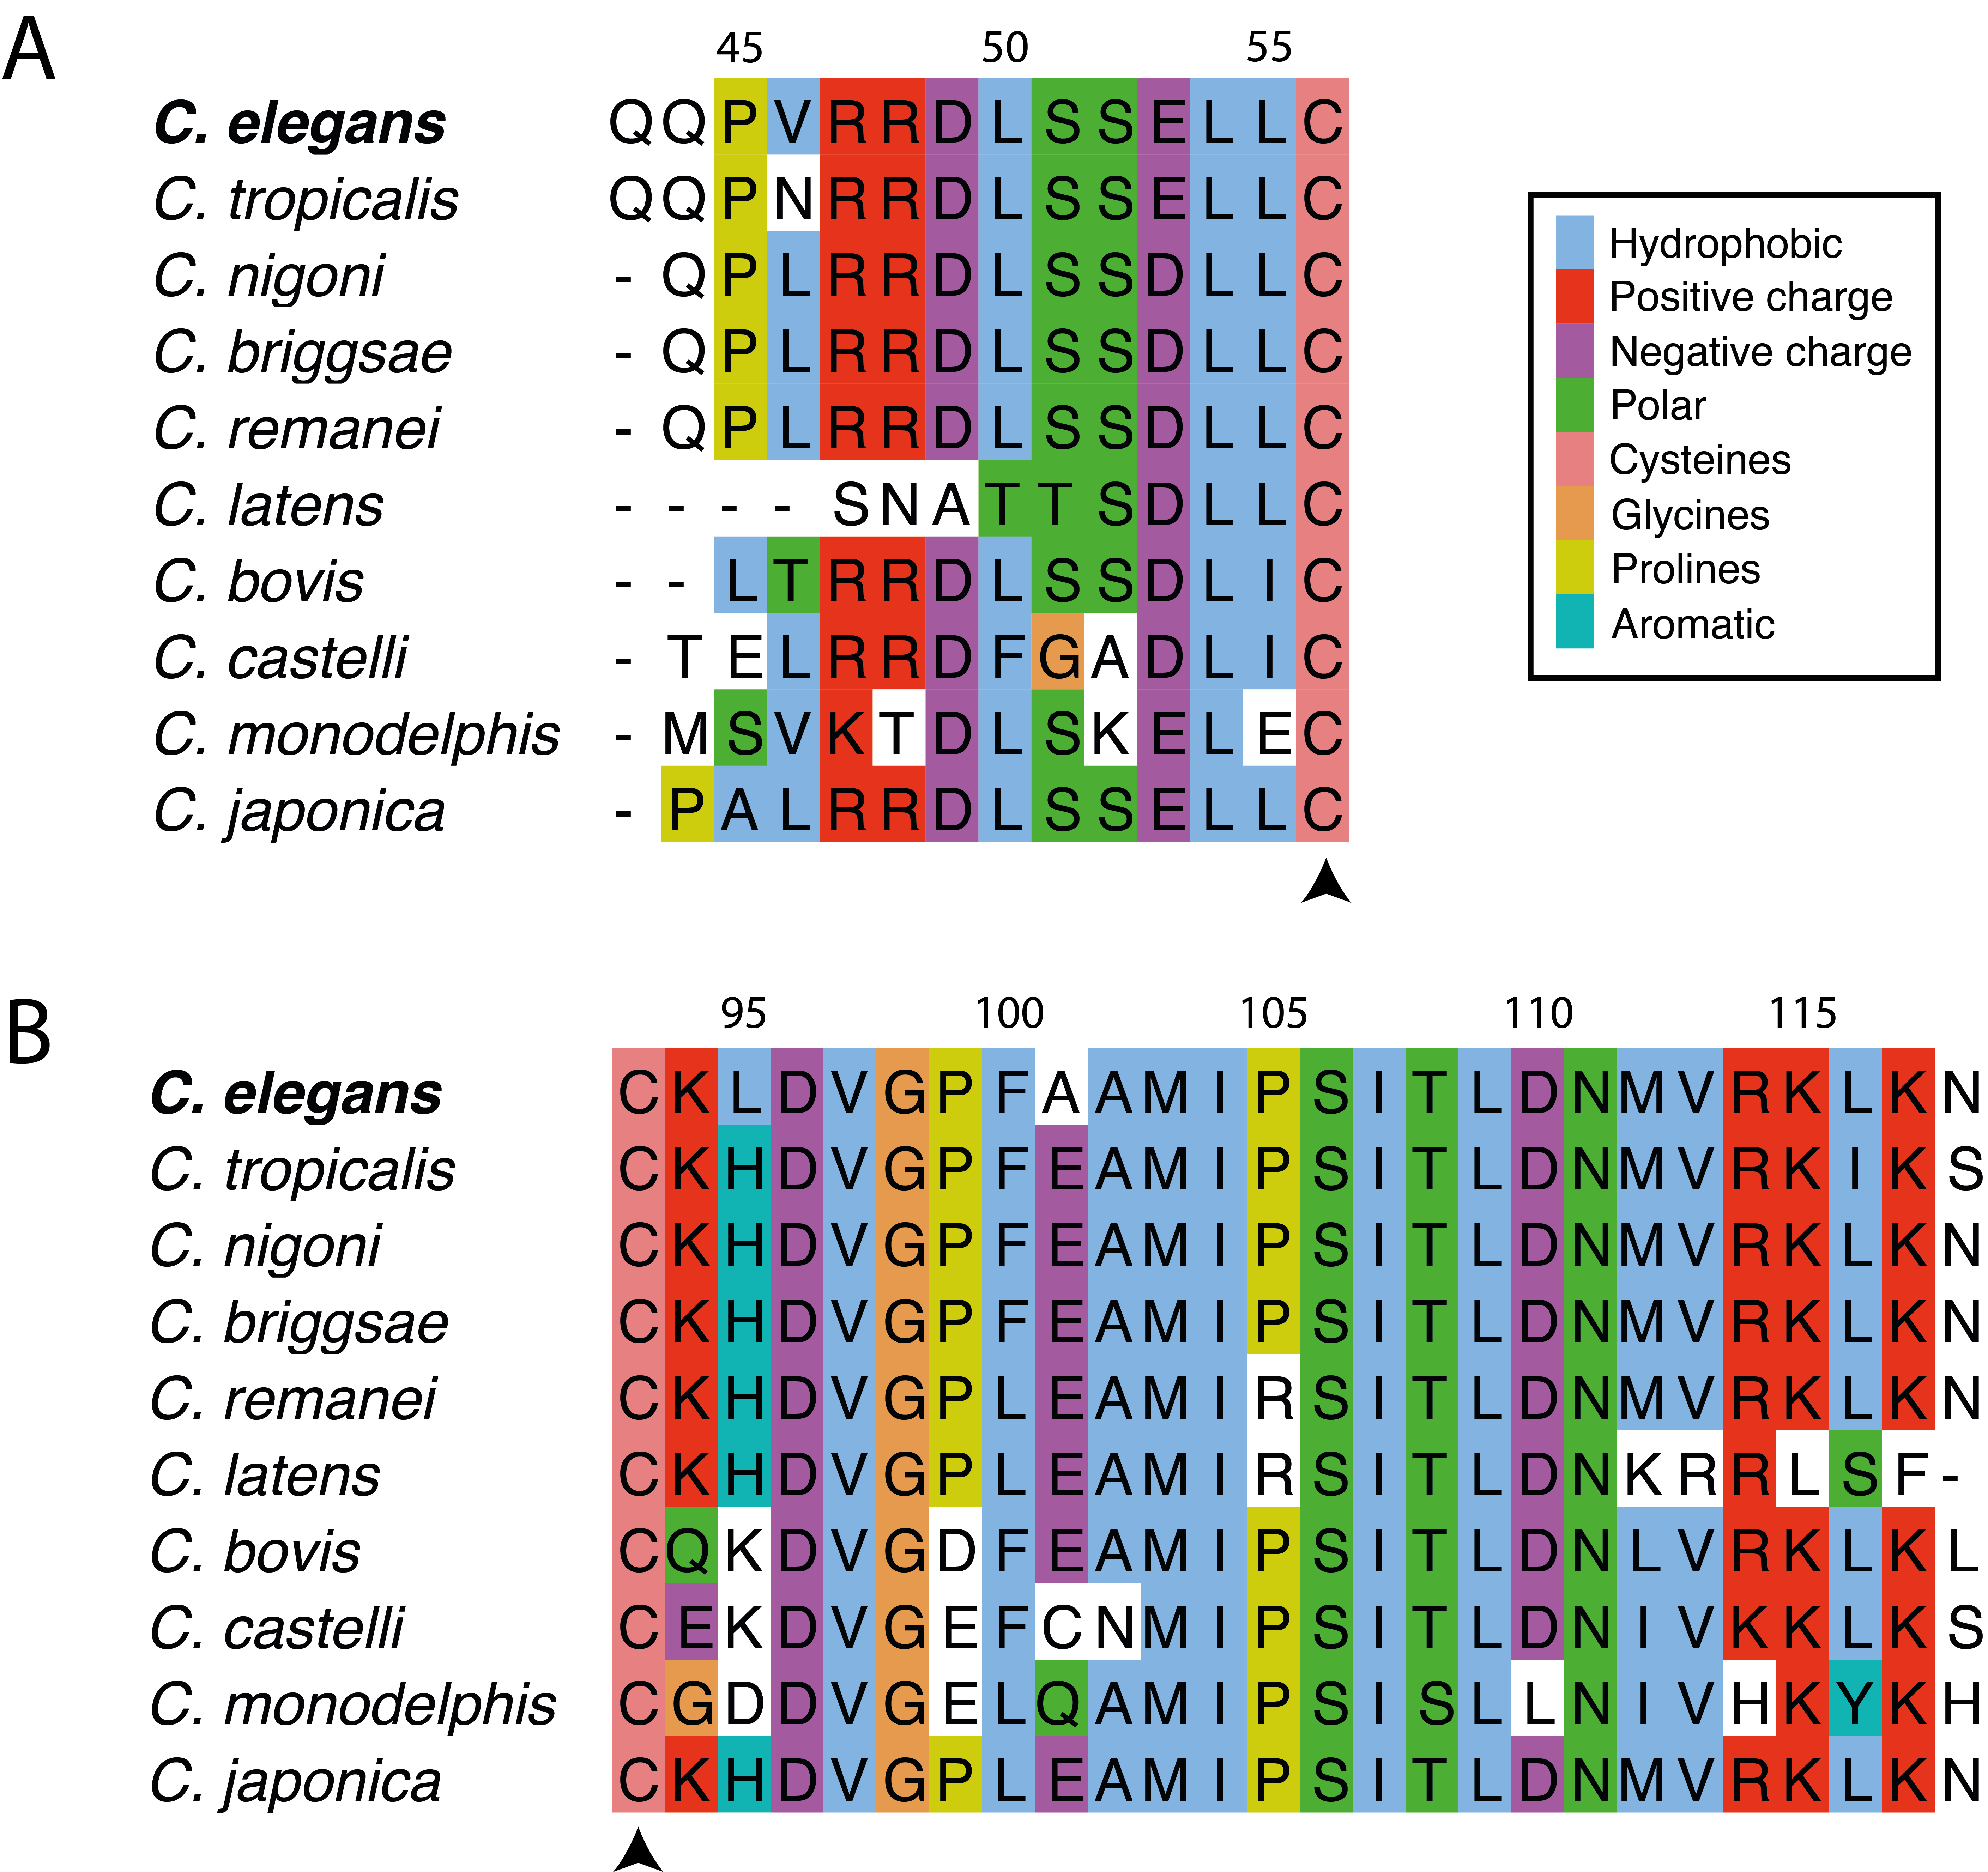
\includegraphics[scale=1]{alignments_par2}
\centering
\mycaption{Alignment of the PAR-2 RING domain N and C helices within the \textit{Caenorhabditis} genus}{
\textbf{(A)} N-helix alignment. Arrowhead indicates first zinc-coordinating cysteine of the core RING domain.
\textbf{(B)} C-helix alignment. Arrowhead indicates final zinc-coordinating cysteine of the core RING domain.
}
\label{fig:alignments_par2}
\end{figure}


\subsection{The PAR-2 RING domain displays concentration-dependent dimerisation in vitro}

\textit{Work in this section was performed with Dave Briggs in Neil McDonald's lab at the Crick}\\

The sequence analysis above suggests that the PAR-2 RING likely has the ability to dimerise. To directly test this, we aimed to purify a fragment of PAR-2  containing the core RING domain and putative N and C helix regions (40-120), and characterise its properties in vitro. We were successfully able to express the fragment in bacteria, and purify it by His pull down, followed by tag removal, ion exchange chromatography and size exclusion chromatography (see Methods).\\

To understand the oligomeric properties of the PAR-2 RING domain in solution, we subjected our purified sample to SEC-MALS, a common approach for characterising the molecular mass and oligomeric state of protein samples. The strategy follows a two step process. Firstly, size exclusion chromatography (SEC), separates particles in a sample based on their size. Larger particles leave the SEC column before smaller particles (i.e. at lower retention volumes). Refractive index scores monitor the concentration of particles leaving the column. Secondly, the eluent flow leaving the SEC column is monitored continuously by a multi-angle light scattering (MALS) instrument, which provides an estimate of the molecular weight of particles based on light scattering properties.\\

We performed five SEC-MALS assays on PAR-2 RING, using sample concentrations of 10, 5, 2, 0.75 and 0.5 mg/ml (\ref{fig:sec_mals}A). In all cases a single peak is observed in refractive index traces, with corresponding molar mass measurements by MALS somewhere between the expected weight of a monomer and a dimer, suggesting that the sample exists in a monomer-dimer equilibrium. Furthermore, mass distributions show clear concentration-dependence, with more concentrated samples giving higher molar mass measurements. This is more clearly visualised in (\ref{fig:sec_mals}B), which shows that the average molecular weight of particles in the sample increases as a function of sample concentration. Overall, this data suggests that the PAR-2 RING domain displays concentration-dependent dimerisation, existing largely as a monomer at low concentrations and mostly dimeric at higher concentrations.\\

\begin{figure}
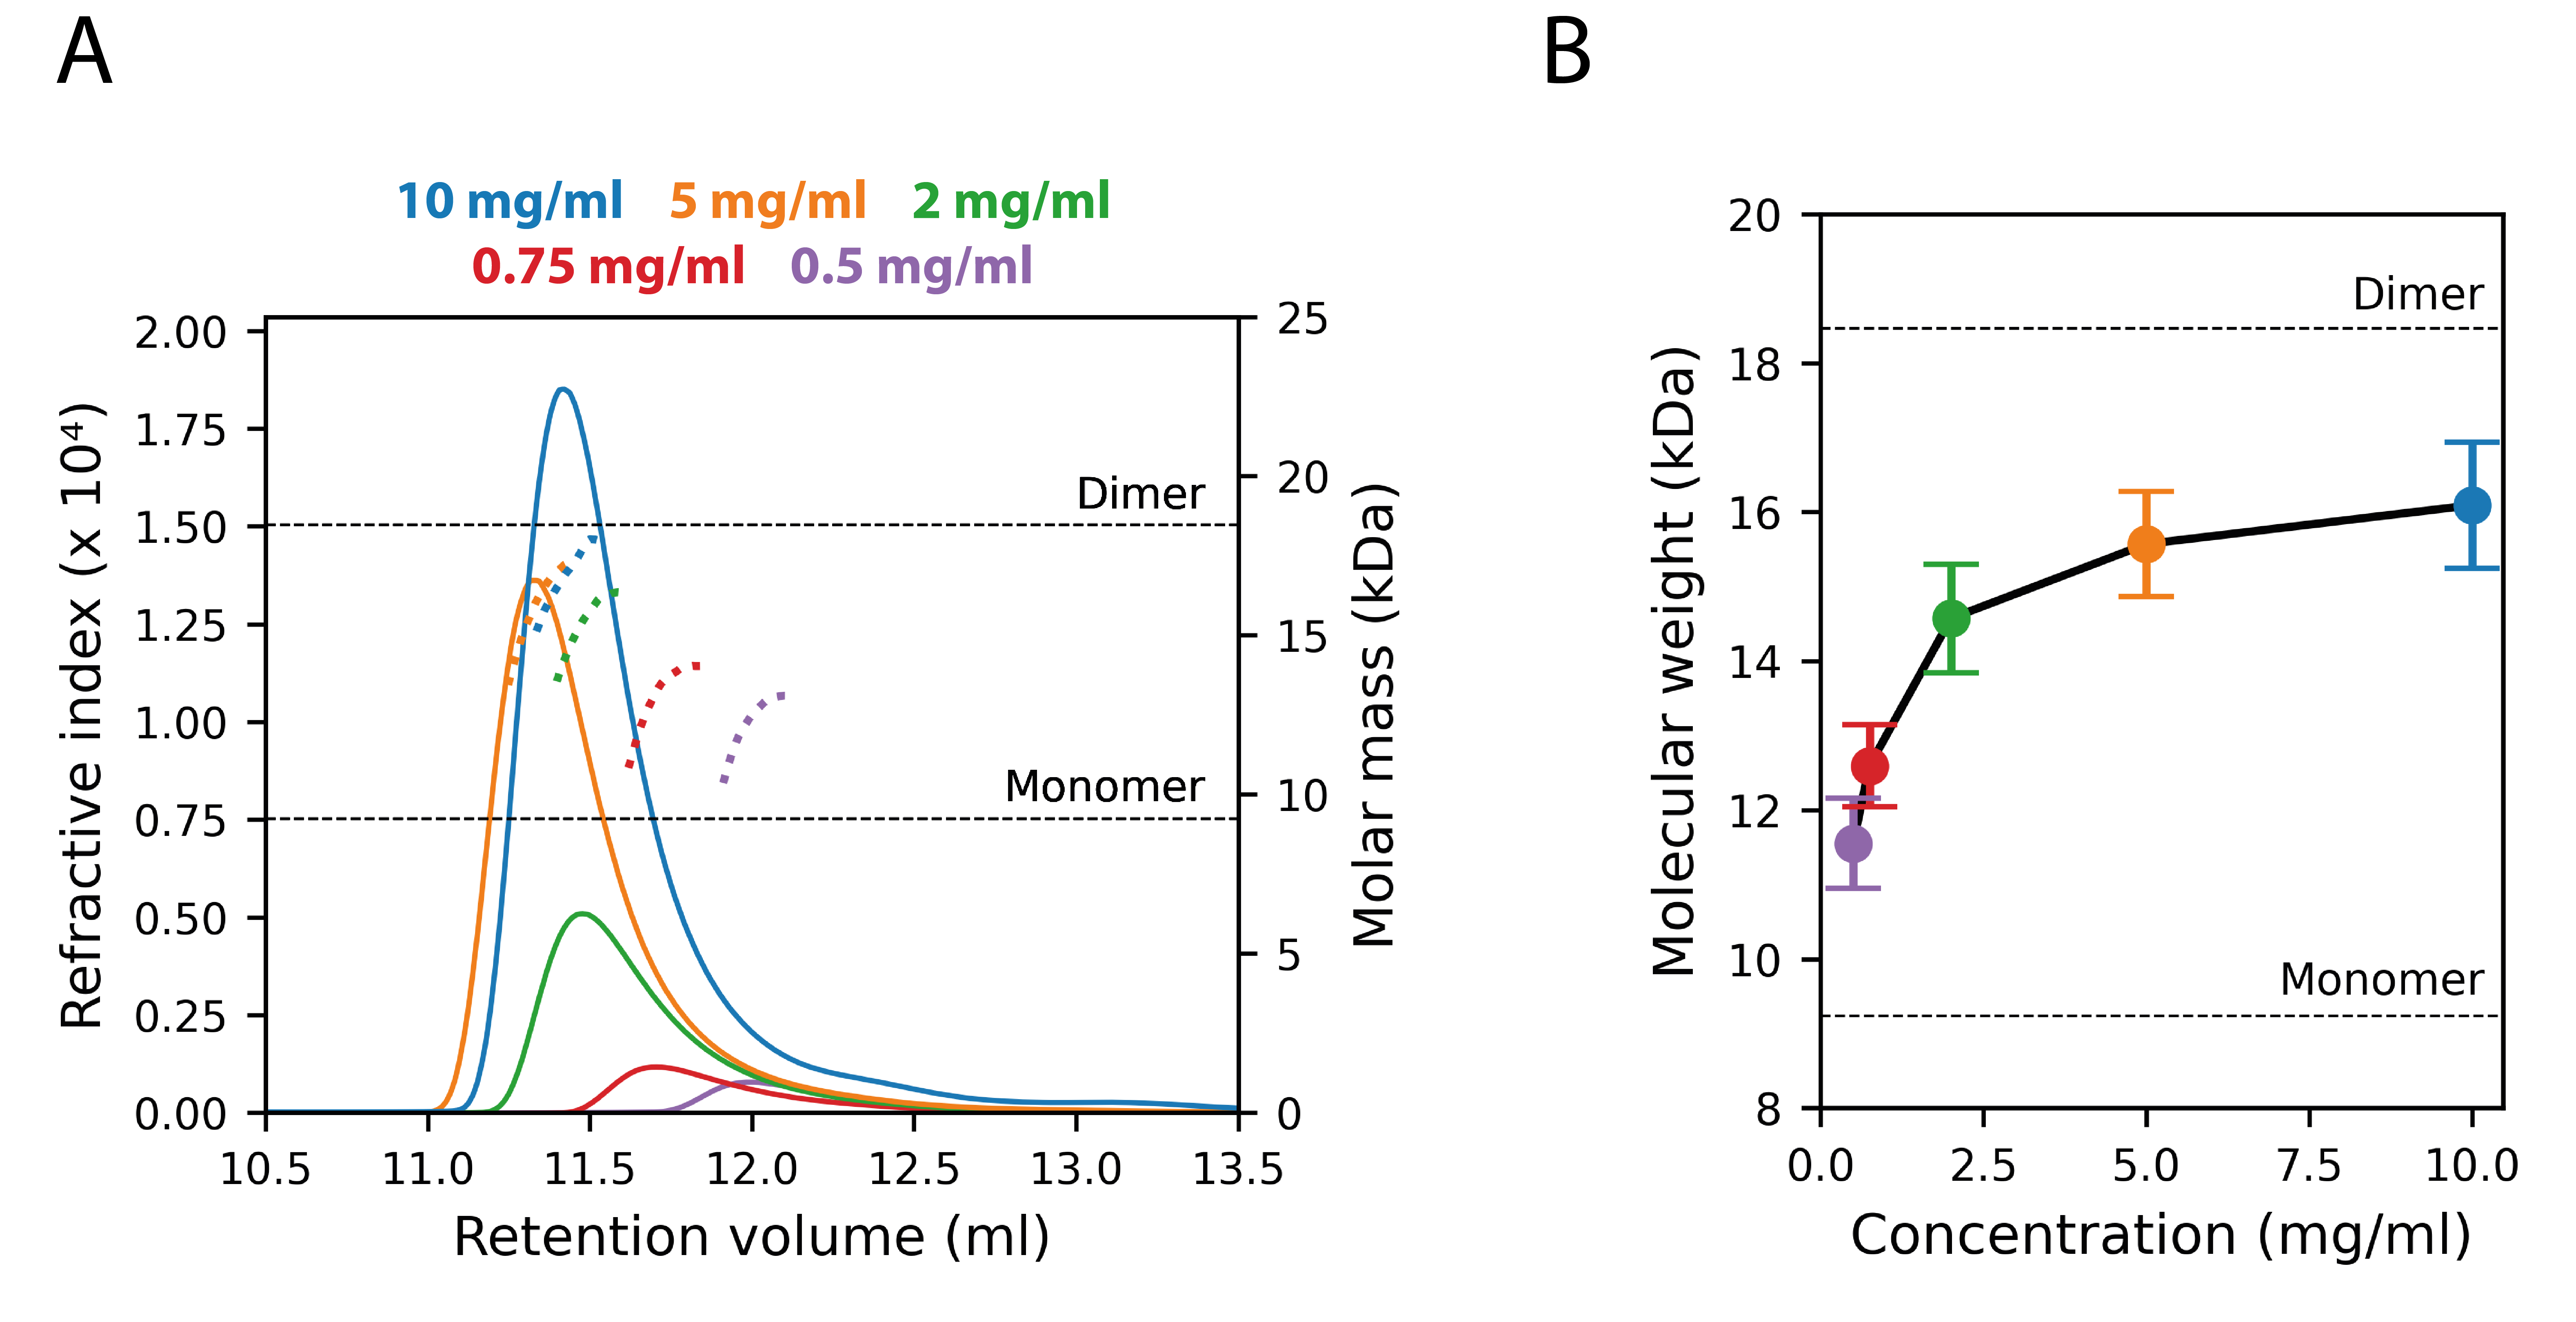
\includegraphics[scale=1]{sec_mals}
\centering
\mycaption{SEC-MALS titration reveals concentration-dependent dimerisation of the PAR-2 RING domain}{
\textbf{(A)} SEC-MALS traces for the PAR-2 RING domain at different concentrations. Solid lines indicate refractive index measurements, dotted lines indicate molar mass measurements. Colour coded by sample concentration. MALS traces are cropped to retention volumes for which refractive index is $>$ 80\% of its peak value.
\textbf{(B)} Molecular weight measurements vs. concentration for the SEC-MALS assays in (A). Note, for samples in a monomer-dimer equilibrium, this represents the average weight of all particles in the sample. Error bars represent measurement uncertainty.
}
\label{fig:sec_mals}
\end{figure}


\subsection{Dimerisation is mediated by 4-helix bundle with hydrophobic core}

To better understand the structural basis of dimerisation, we aimed to resolve the structure of the PAR-2 RING domain dimer by X-ray crystallography. We successfully purified sufficient quantities of protein to set up crystal screens, but have so far been unsuccessful in generating crystals. Nevertheless, owing to recent advances in protein structure prediction tools, such as AlphaFold \citep{Jumper2021}, we can get good estimates of the protein structures based on their sequence of amino acids.\\

I used AlphaFold to predict the structure of the PAR-2 RING domain dimer (residues 40-120 of the protein). The predicted structure (\cref{fig:ring_alphafold}) resembles the common structure of RING domain dimers, characterised by a four-helix bundle consisting of an N and C helix from each of the two monomers (\cref{fig:ring_alphafold}B). Within this bundle, we see a characteristic pattern of inwards facing hydrophobic residues (\cref{fig:ring_alphafold}D). Confidence scores, as measured by the AlphaFold metric pLDDT (predicted local distance difference test), are high throughout the structured region of the model (\cref{fig:ring_alphafold}C).\\

\begin{figure}
\includegraphics[scale=0.9]{ring_alphafold}
\centering
\mycaption{AlphaFold prediction for the 3D structure of the PAR-2 RING domain dimer}{
\textbf{(A)} 3D structure colour coded by chain.
\textbf{(B)} 3D structure with N and C helices highlighted.
\textbf{(C)} 3D structure colour coded by pLDDT, an AlphaFold metric for prediction confidence.
\textbf{(D)} 3D structure colour coded by hydrophobicity, with red indicating more hydrophobic and white indicating less hydrophobic. Inset shows enlarged view of the 4-helix bundle, showing internally facing hydrophobic residues.
}
\label{fig:ring_alphafold}
\end{figure}

I also generated predictions for the PAR-2 RING across the \textit{Caenorhabditis} genus (\cref{fig:ring_alphafold_species}). These show that the 4-helix bundle structure is predicted to be largely conserved across the genus, although confidence scores within this region are variable. A major exception is \textit{C. latens}, which is predicted to form no bundle at all. This is compatible with a lack of hydrophobic residues at the sites in the common N and C helix regions (\cref{fig:alignments_par2}). It's likely that, unlike other species, the RING domain of \textit{C. latens} PAR-2 is monomeric.\\

\begin{figure}
\includegraphics[scale=0.9]{ring_alphafold_species}
\centering
\mycaption{AlphaFold predictions for the PAR-2 RING domain across the \textit{Caenorhabditis} genus}{
Colour coded by pLDDT.
}
\label{fig:ring_alphafold_species}
\end{figure}

Given that dimerisation is predicted to be mediated by a hydrophobic interface within a 4-helix bundle, we would expect that mutations to hydrophobic residues within this region should disrupt dimerisation, as has been shown previously for several RING domains \citep{Koliopoulos2016, Rojas-Fernandez2014, Liew2010}. Unlike mutations to zinc-coordinating cysteines, which completely misfold the domain, mutations to this interface should preserve the tertiary structure of the domain and specifically disrupt dimerisation. I identified L109, predicted to be found in the C-helix as a likely important site (\cref{fig:l109r_sec_mals}A), and L109R as a likely disruptive mutation. As we did for the wild-type RING domain, we expressed the mutant allele in bacteria and purified it using the same protocol. SEC-MALS shows that this mutant has the expected molecular weight of an entirely monomeric population (\cref{fig:l109r_sec_mals}A). By contrast, wild type RING at an equivalent concentration (\cref{fig:sec_mals}A, 0.75 mg/ml) is partially dimeric.\\

\begin{figure}
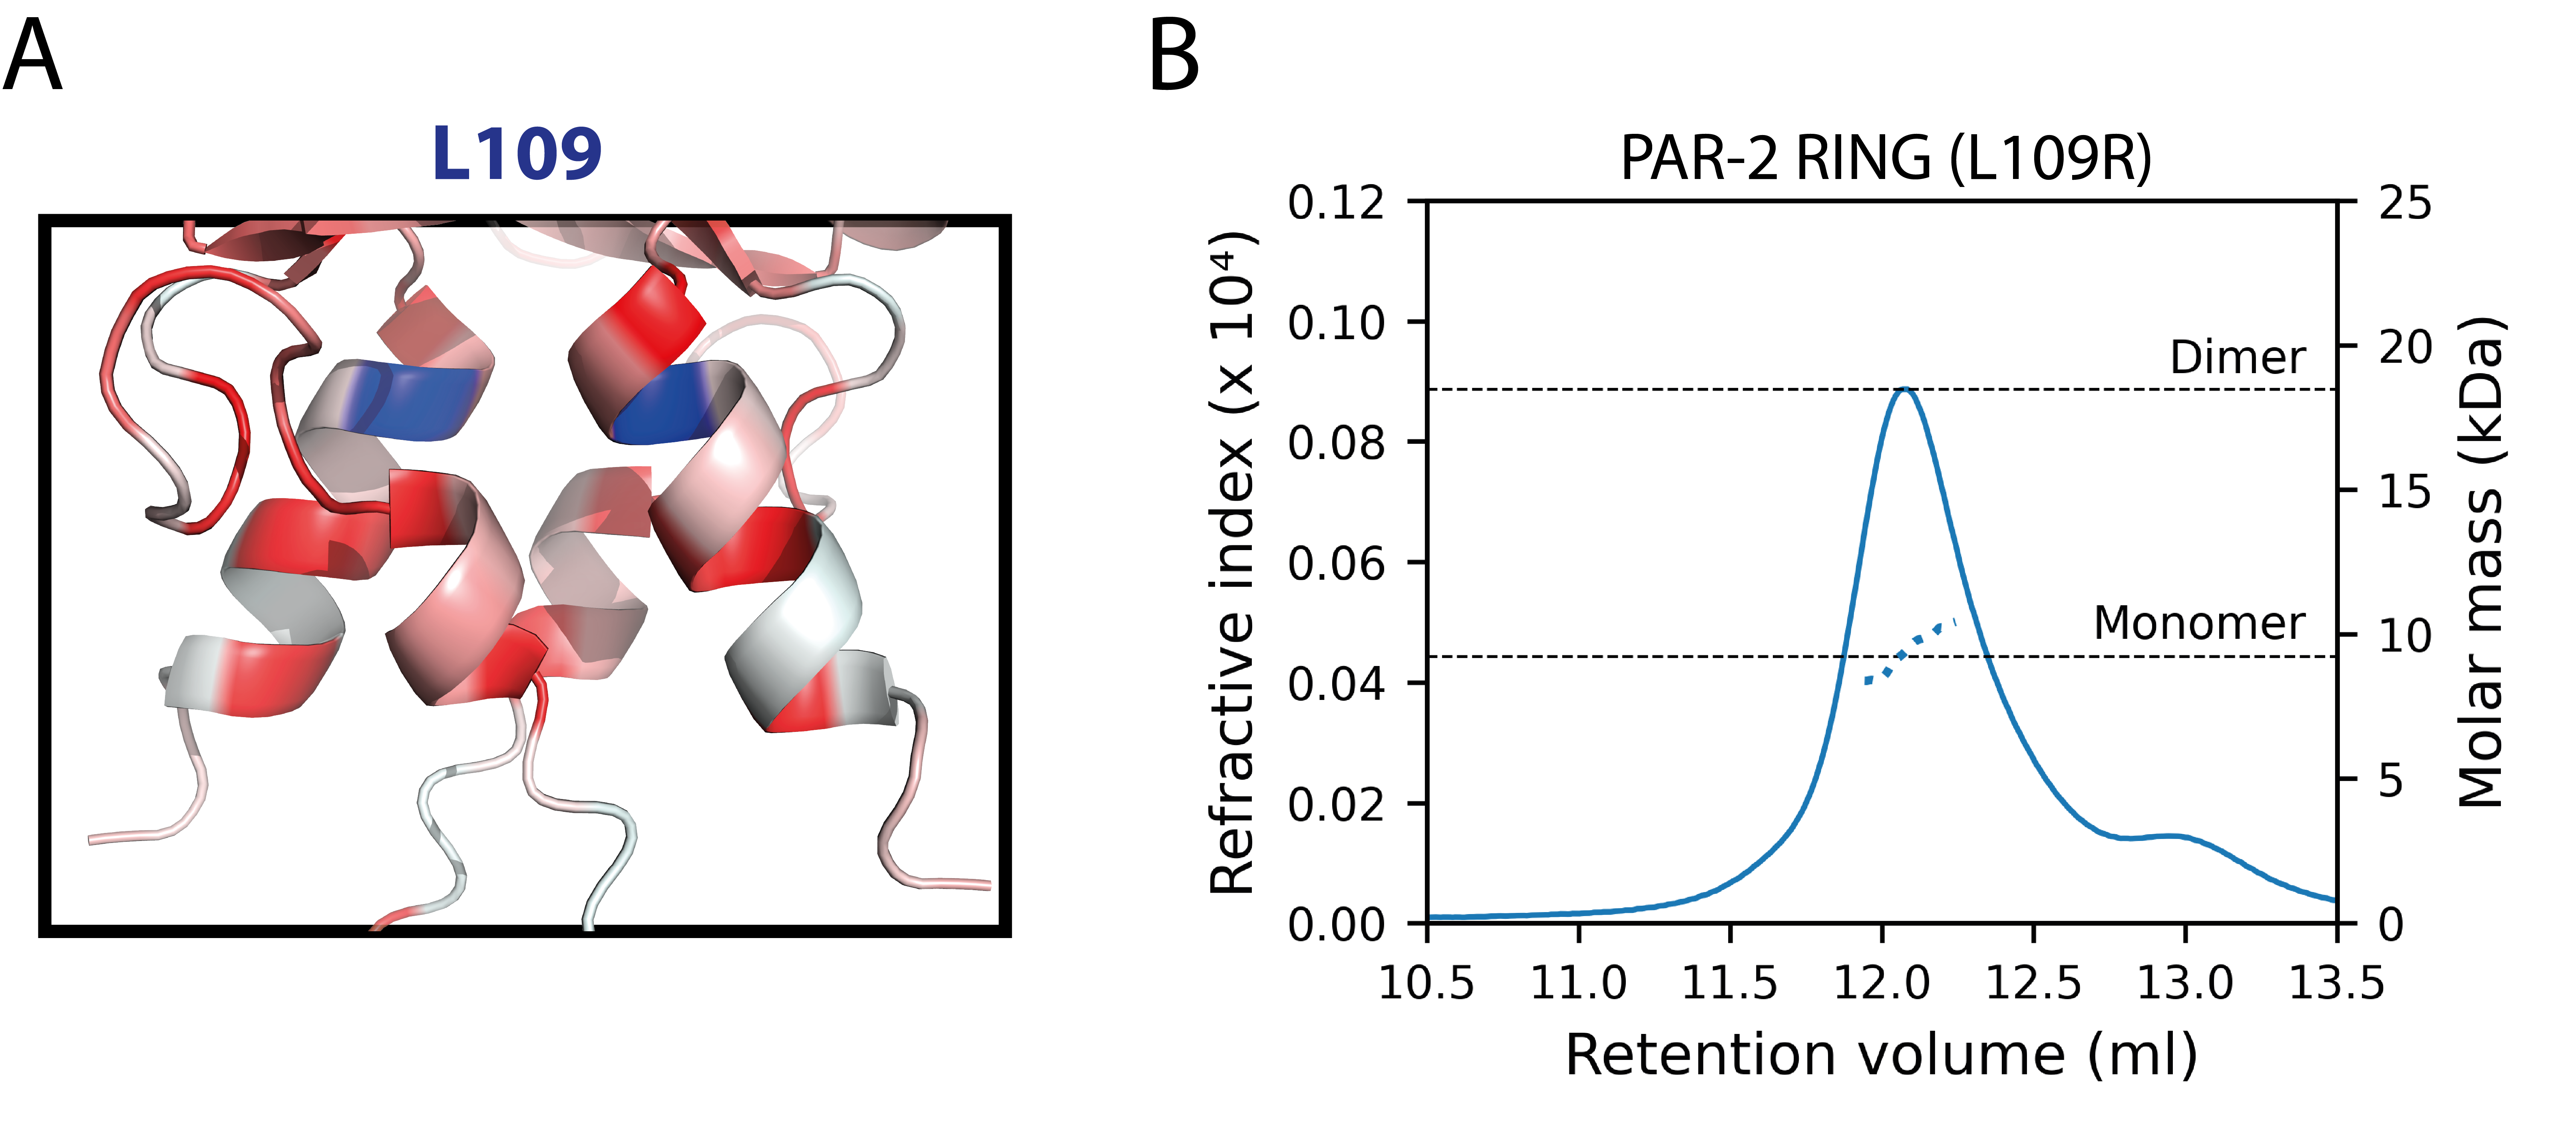
\includegraphics[scale=1]{l109r_sec_mals}
\centering
\mycaption{Mutation of residue at hydrophobic interface disrupts PAR-2 RING domain dimerisation}{
\textbf{(A)} Position of the L109 site within the 4-helix bundle of the PAR-2 RING domain. L109 site highlighted in blue, other residues coloured by hydrophobicity.
\textbf{(B)} SEC-MALS trace for PAR-2 RING (L109R). Solid line indicates refractive index, dotted line indicates molar mass. Sample concentration approx 0.75 mg/ml.
}
\label{fig:l109r_sec_mals}
\end{figure}

As a further test, we attempted to express and purify a C56S mutant RING domain for SEC-MALS. However, we found the protein to be unstable in vitro and were unable to purify it significant quantities to perform the assay, which is a common problem for unfolded proteins.\\

\subsection{Cytoplasmic PAR-2  does not self-associate in vivo}

The in vitro results described so far suggest that the PAR-2 RING domain displays concentration-dependent dimerisation. In vivo, PAR-2 concentrations are relatively low in the cytoplasm, but local concentrations are greatly enhanced upon membrane association. To investigate the potential role for RING-mediated PAR-2 dimerisation in vivo, I considered the cytoplasmic and membrane fractions separately, and devised two in vivo assays designed to test the dimeric state of PAR-2 in the cytoplasm and on the membrane.\\

To test the dimeric state of cytoplasmic PAR-2, I devised an in vivo pull-down assay based on dual labelling of PAR-2 with two different fluorophores (\cref{fig:tomm20_schematic}). Expressing PAR-2 with a mix of GFP and mCherry fluorophores means that, were cytoplasmic PAR-2 to form dimers, a mixed population of GFP/GFP, GFP/mCherry and mCherry/mCherry dimers would be expected to be present within the cytoplasm. Thus, forced relocalisation of GFP::PAR-2 to a particular location in the cell should result in a detectable signal mCherry::PAR-2 at that location. A similar assay was used previously by \textcite{Reich2019}, who demonstrated a stable interaction between PAR-6 and PKC-3, through forced localisation of GFP::PKC-3 to the plasma membrane with a plasma membrane tethered GFP binding protein (GBP). (In this case the plasma membrane was a suitable target because, under the conditions of the assay, PAR-6/PKC-3 do not normally bind to the plasma membrane). Here, I propose a similar approach, relying instead on recruitment to mitochondrial membranes within the cell. Mitochondrial membranes are dense within the \textit{C. elegans} zygote \citep{Dinkelmann2003}, and can be probed easily with a localisation signal from the TOMM-20 protein \citep{Watanabe2011}.\\

\begin{figure}
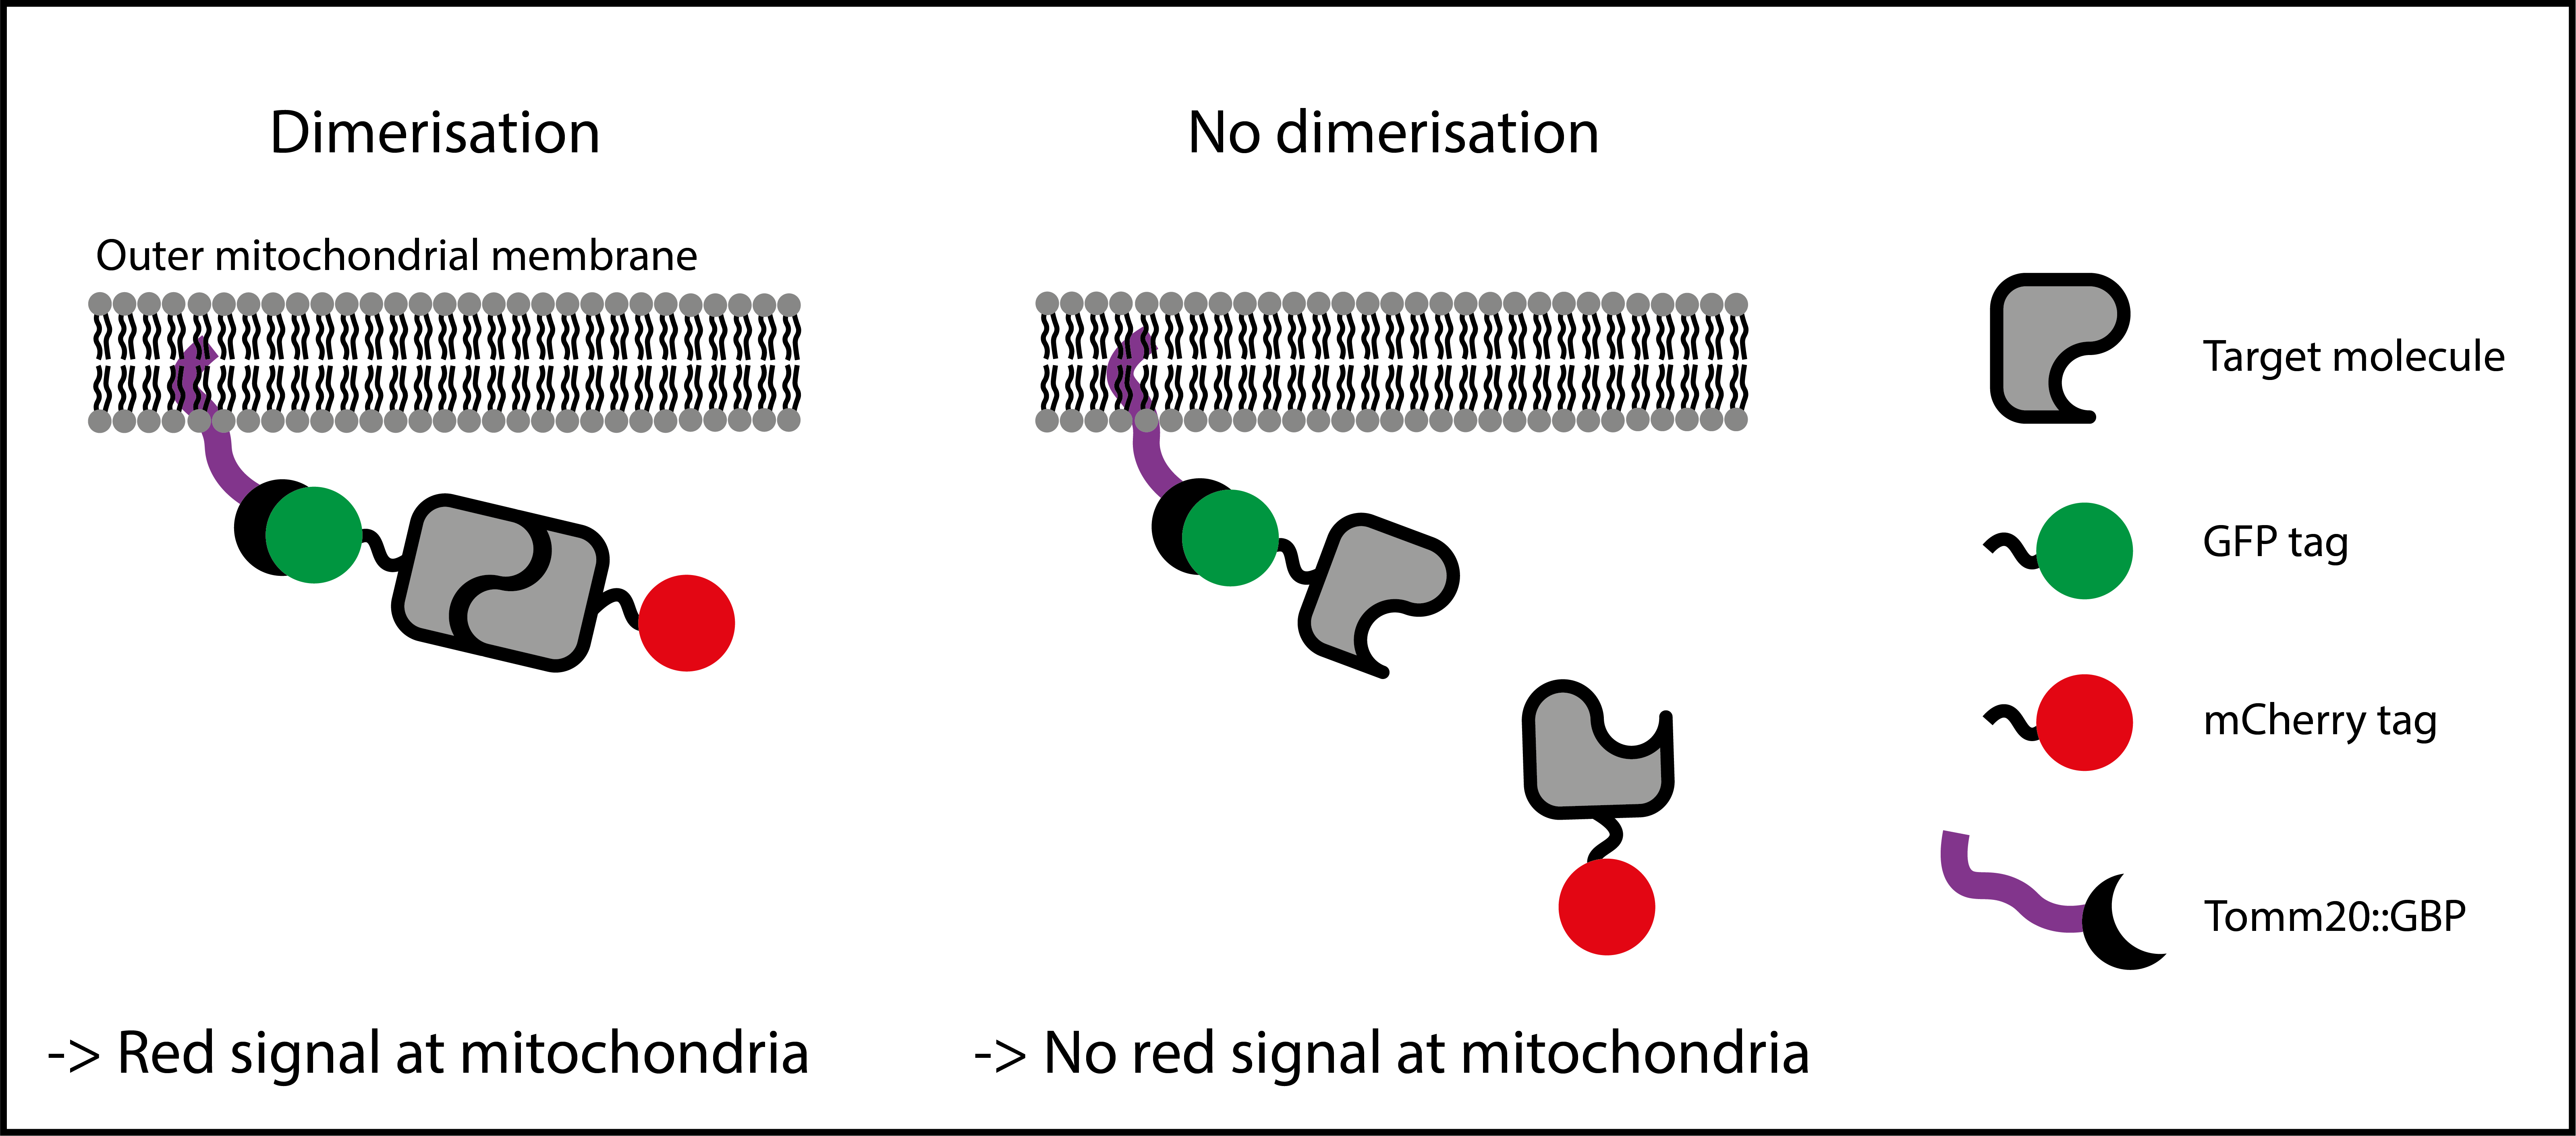
\includegraphics[scale=0.95]{tomm20_schematic}
\centering
\mycaption{Schematic of an in vivo dimerisation assay involving the mitochondrial probe TOMM-20}{
}
\label{fig:tomm20_schematic}
\end{figure}

To first test the potential utility of this method, I built a TOMM-20::GBP probe tagged with mKate, and introduced this into the worm by CRISPR. Crossing this line to a GFP::PAR-2 expressing line, and imaging the F1s (heterozygous for both GFP::PAR-2 and the probe), shows that the probe is well expressed, displays the expected mitochondrial localisation pattern, and is able to recruit GFP::PAR-2 to the mitochondria (\cref{fig:tomm20_merge}).\\

\begin{figure}
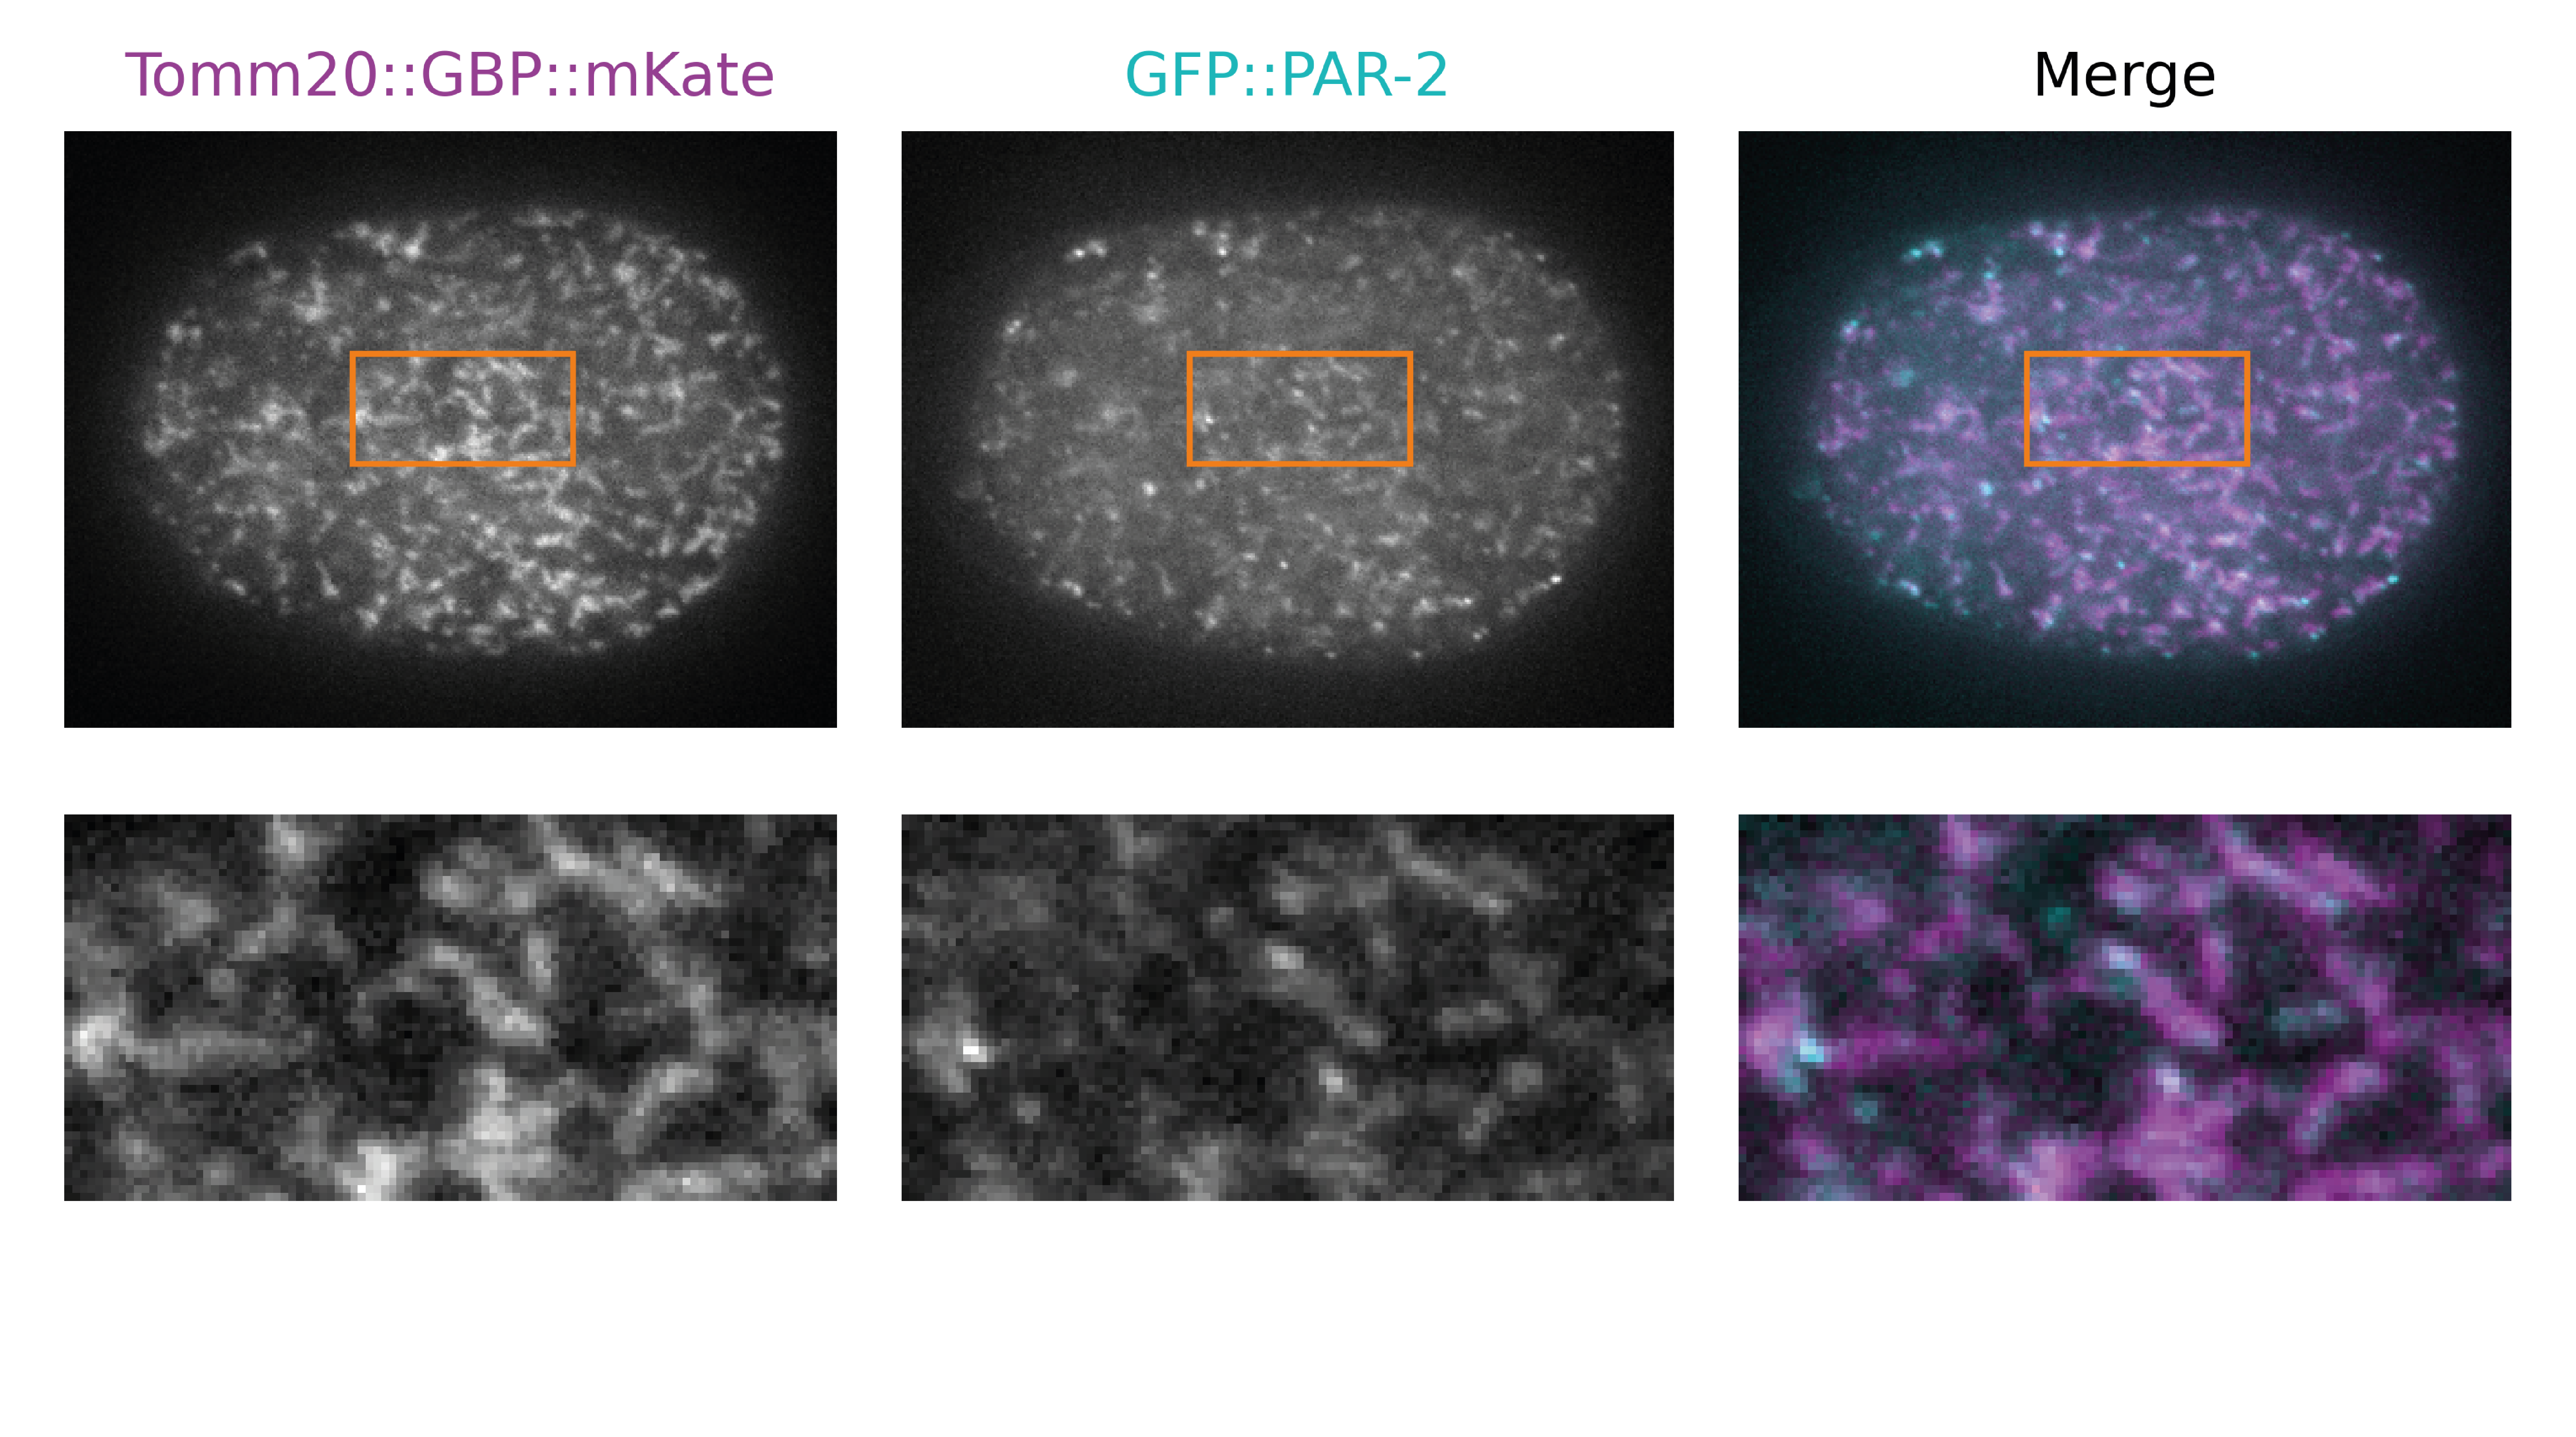
\includegraphics[scale=0.95]{tomm20_merge}
\centering
\mycaption{Mitochondrial GFP nanobody pulls GFP-tagged PAR-2 to mitochondria}{
Images of a zygote expressing Tomm20::GBP::mKate and GFP::PAR-2.
GFP channel image is not autofluorescence corrected. Shows a view between the midplane and cortex, as this gives a clearer signal for mitochondria.
}
\label{fig:tomm20_merge}
\end{figure}

To perform the proposed dimerisation assay, I next attempted to build an untagged version of the mitochondria probe (lacking mKate). Whilst I was successfully able to  introduce the construct into the genome of the worm, I found that this untagged probe failed to recruit any GFP::PAR-2 to the mitochondria, likely indicating that the probe failed to express. This suggests that the mKate tag may be stabilising expression of the full construct, possibly due to the presence of introns within the mKate sequence. As an alternative method to free up the red channel, I introduced a point mutation into mKate by CRISPR designed to disrupt the chromophore region, which is required for fluorescence \citep{Pletnev2008}. This construct, by contrast, was well expressed and, like the tagged parent construct, able to pull GFP::PAR-2 to the mitochondria. Next, I crossed this line to a line expressing mCherry::PAR-2 at the endogenous locus, homozygosing both constructs. I then crossed the resulting line to a line homozygous for endogenous GFP::PAR-2, giving F1s heterozygous for GFP/mCherry PAR-2, and heterozygous for the mitochondrial probe.  Imaging embryos from these F1s showed that, whereas GFP::PAR-2 is fully pulled to the mitochondria, there is no detectable colocalisation with mCherry::PAR-2, which retains a normal pattern of cytoplasmic and cortical localisation (\cref{fig:tomm20_assay}). Overall, as mCherry signal is not observed at the mitochondria, the result implies that cytoplasmic PAR-2 is largely or entirely monomeric.\\

\begin{figure}
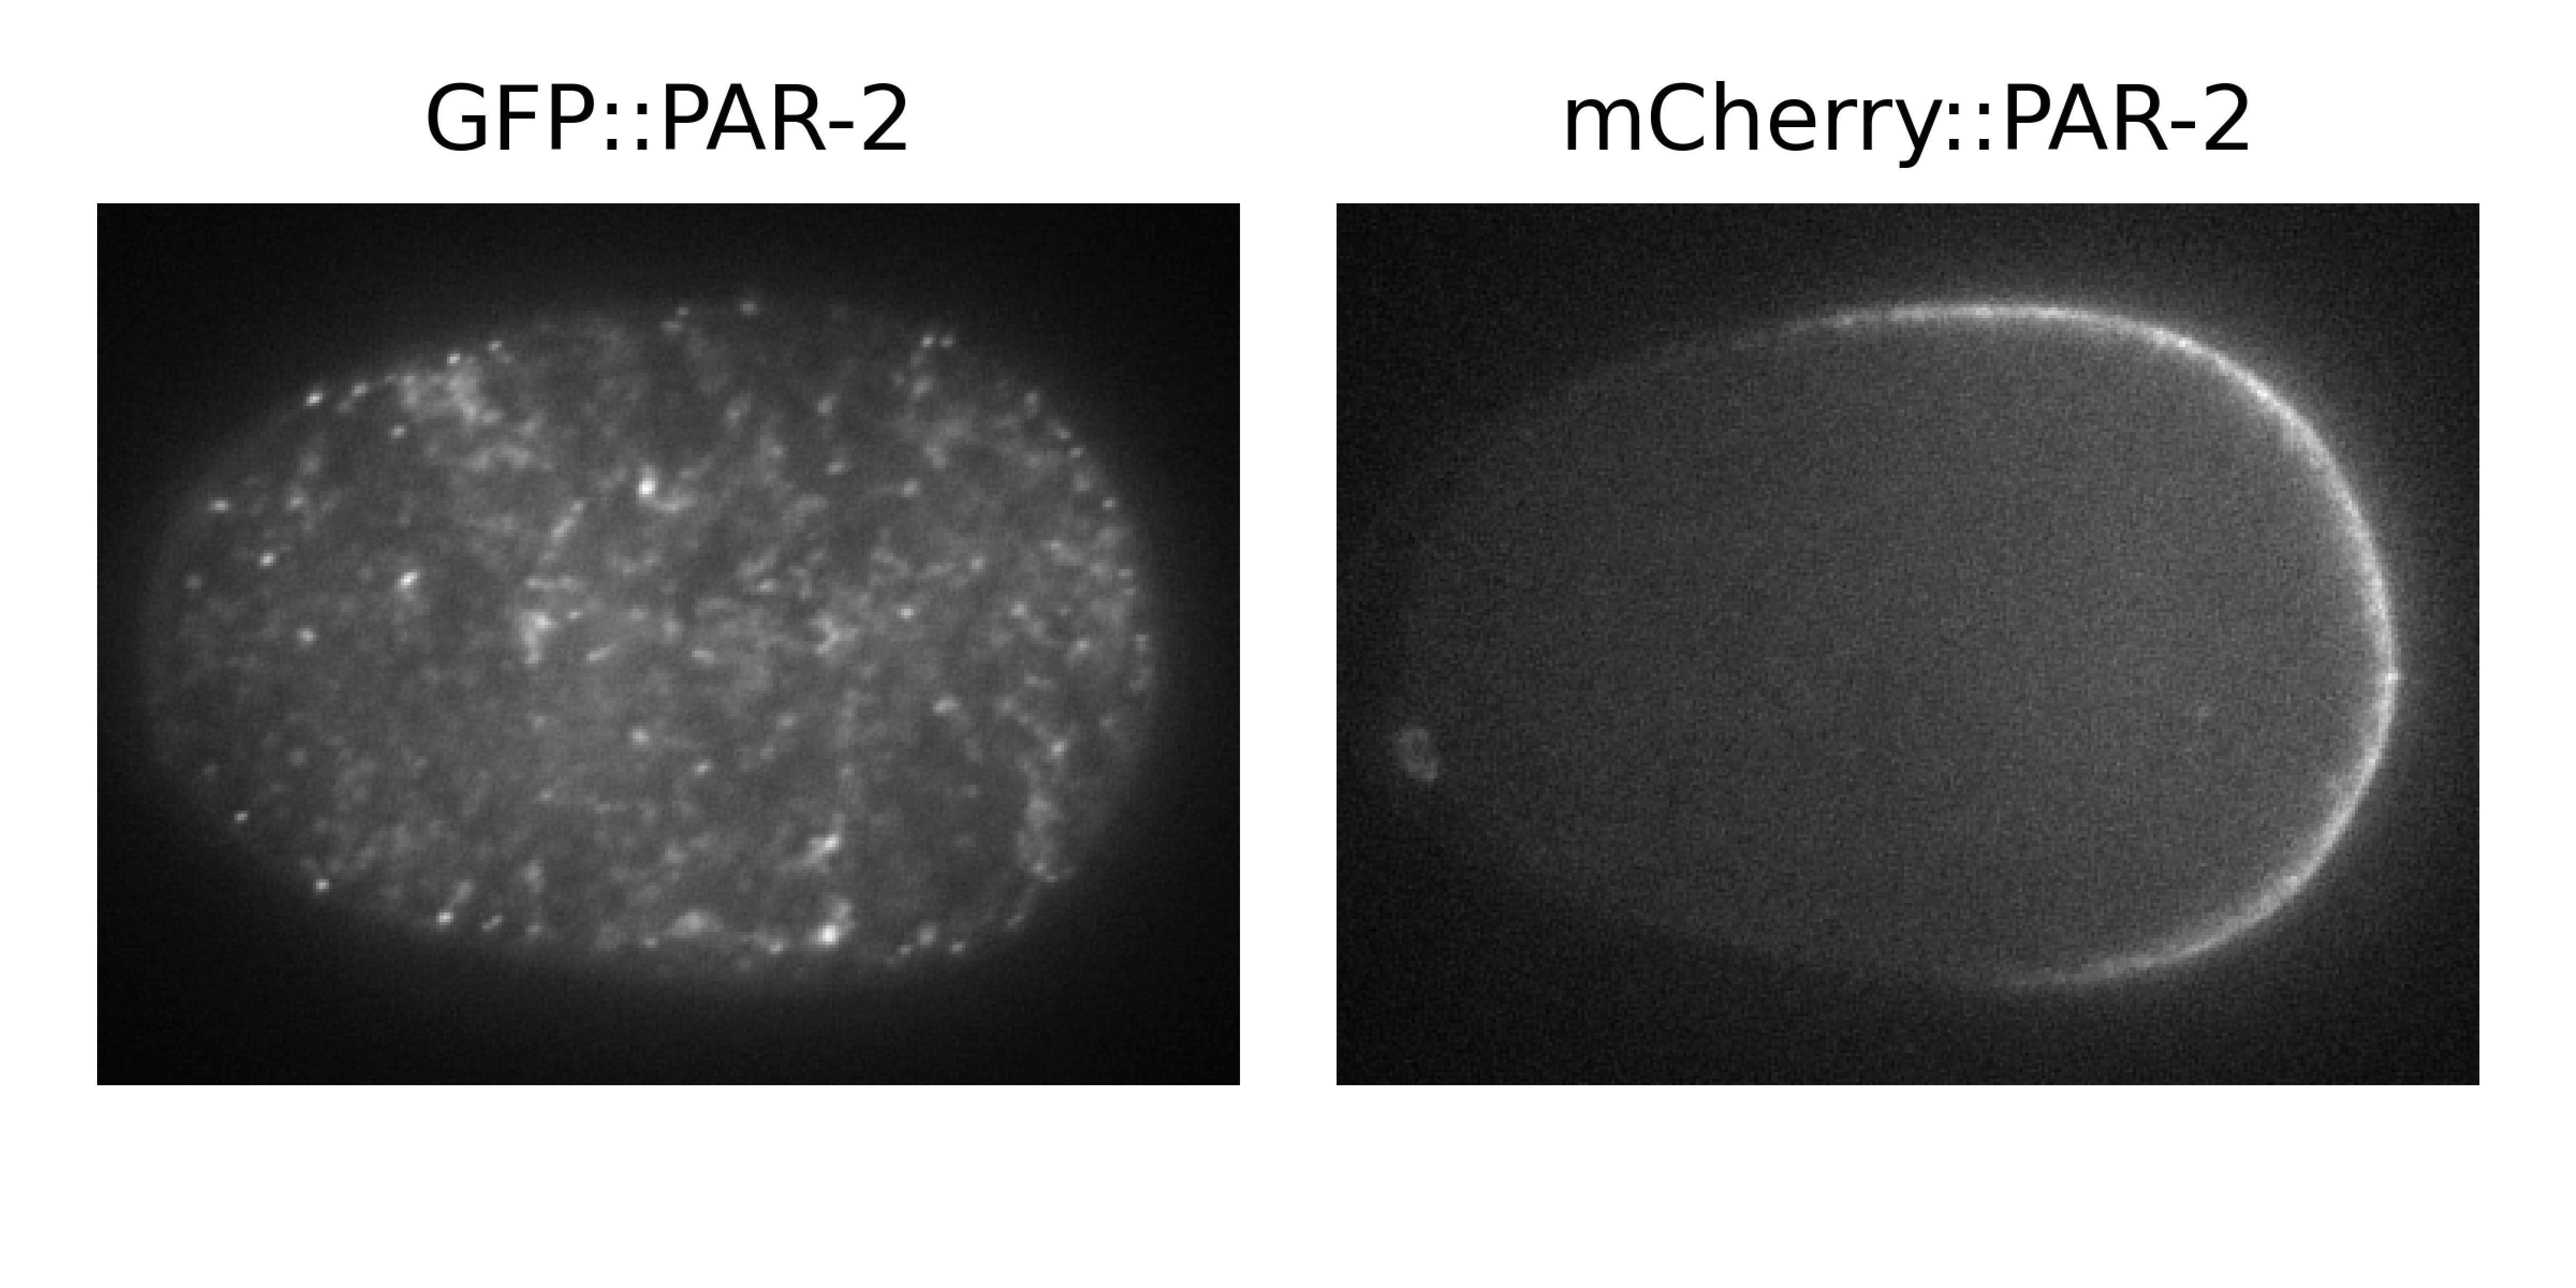
\includegraphics[scale=1]{tomm20_assay}
\centering
\mycaption{In vivo dimerisation assay shows that PAR-2 does not constitutively dimerise in vivo}{
Images of GFP::PAR-2 and mCherry::PAR-2 in a line heterozygous for GFP/mCherry PAR-2 and heterozygous for TOMM-20::GBP. GFP channel image is not autofluorescence corrected. Shows a view between midplane and cortex as this gives a clearer signal for mitochondria.
}
\label{fig:tomm20_assay}
\end{figure}


\subsection{Membrane-enriched PAR-2 self-associates in vivo}

I next aimed to test the ability of the PAR-2 RING to dimerise on the membrane, where concentrations are greatly enhanced compared to the cytoplasm. To investigate this, I used a pleckstrin homology (PH) plasma membrane probe to tether a RING-containing fragment of PAR-2 (1-177) to the plasma membrane. Should this construct be capable of dimerisation, we would expect some degree of dimerisation with endogenous PAR-2, and therefore preferential enrichment in the posterior of the cell. The construct is poorly expressed, but visible after autofluorescence correction by SAIBR. Whilst PH alone is uniform on the membrane, tethering it to the PAR-2 RING domain causes clear enrichment in the posterior, which suggests an interaction with endogenous PAR-2 (\cref{fig:ph_ring}). A C56S mutant construct, by contrast, shows a reduced degree of polarity compared to the wild type probe. Furthermore, the RING fragment alone shows no membrane localisation, suggesting that membrane enrichment is first required to permit dimerisation with endogenous PAR-2 (\cref{fig:ring_fragment_in_vivo}). This is in line with a previous study which showed a similar result using the same RING domain fragment \citep{Hao2006}.\\

\begin{figure}[!h]
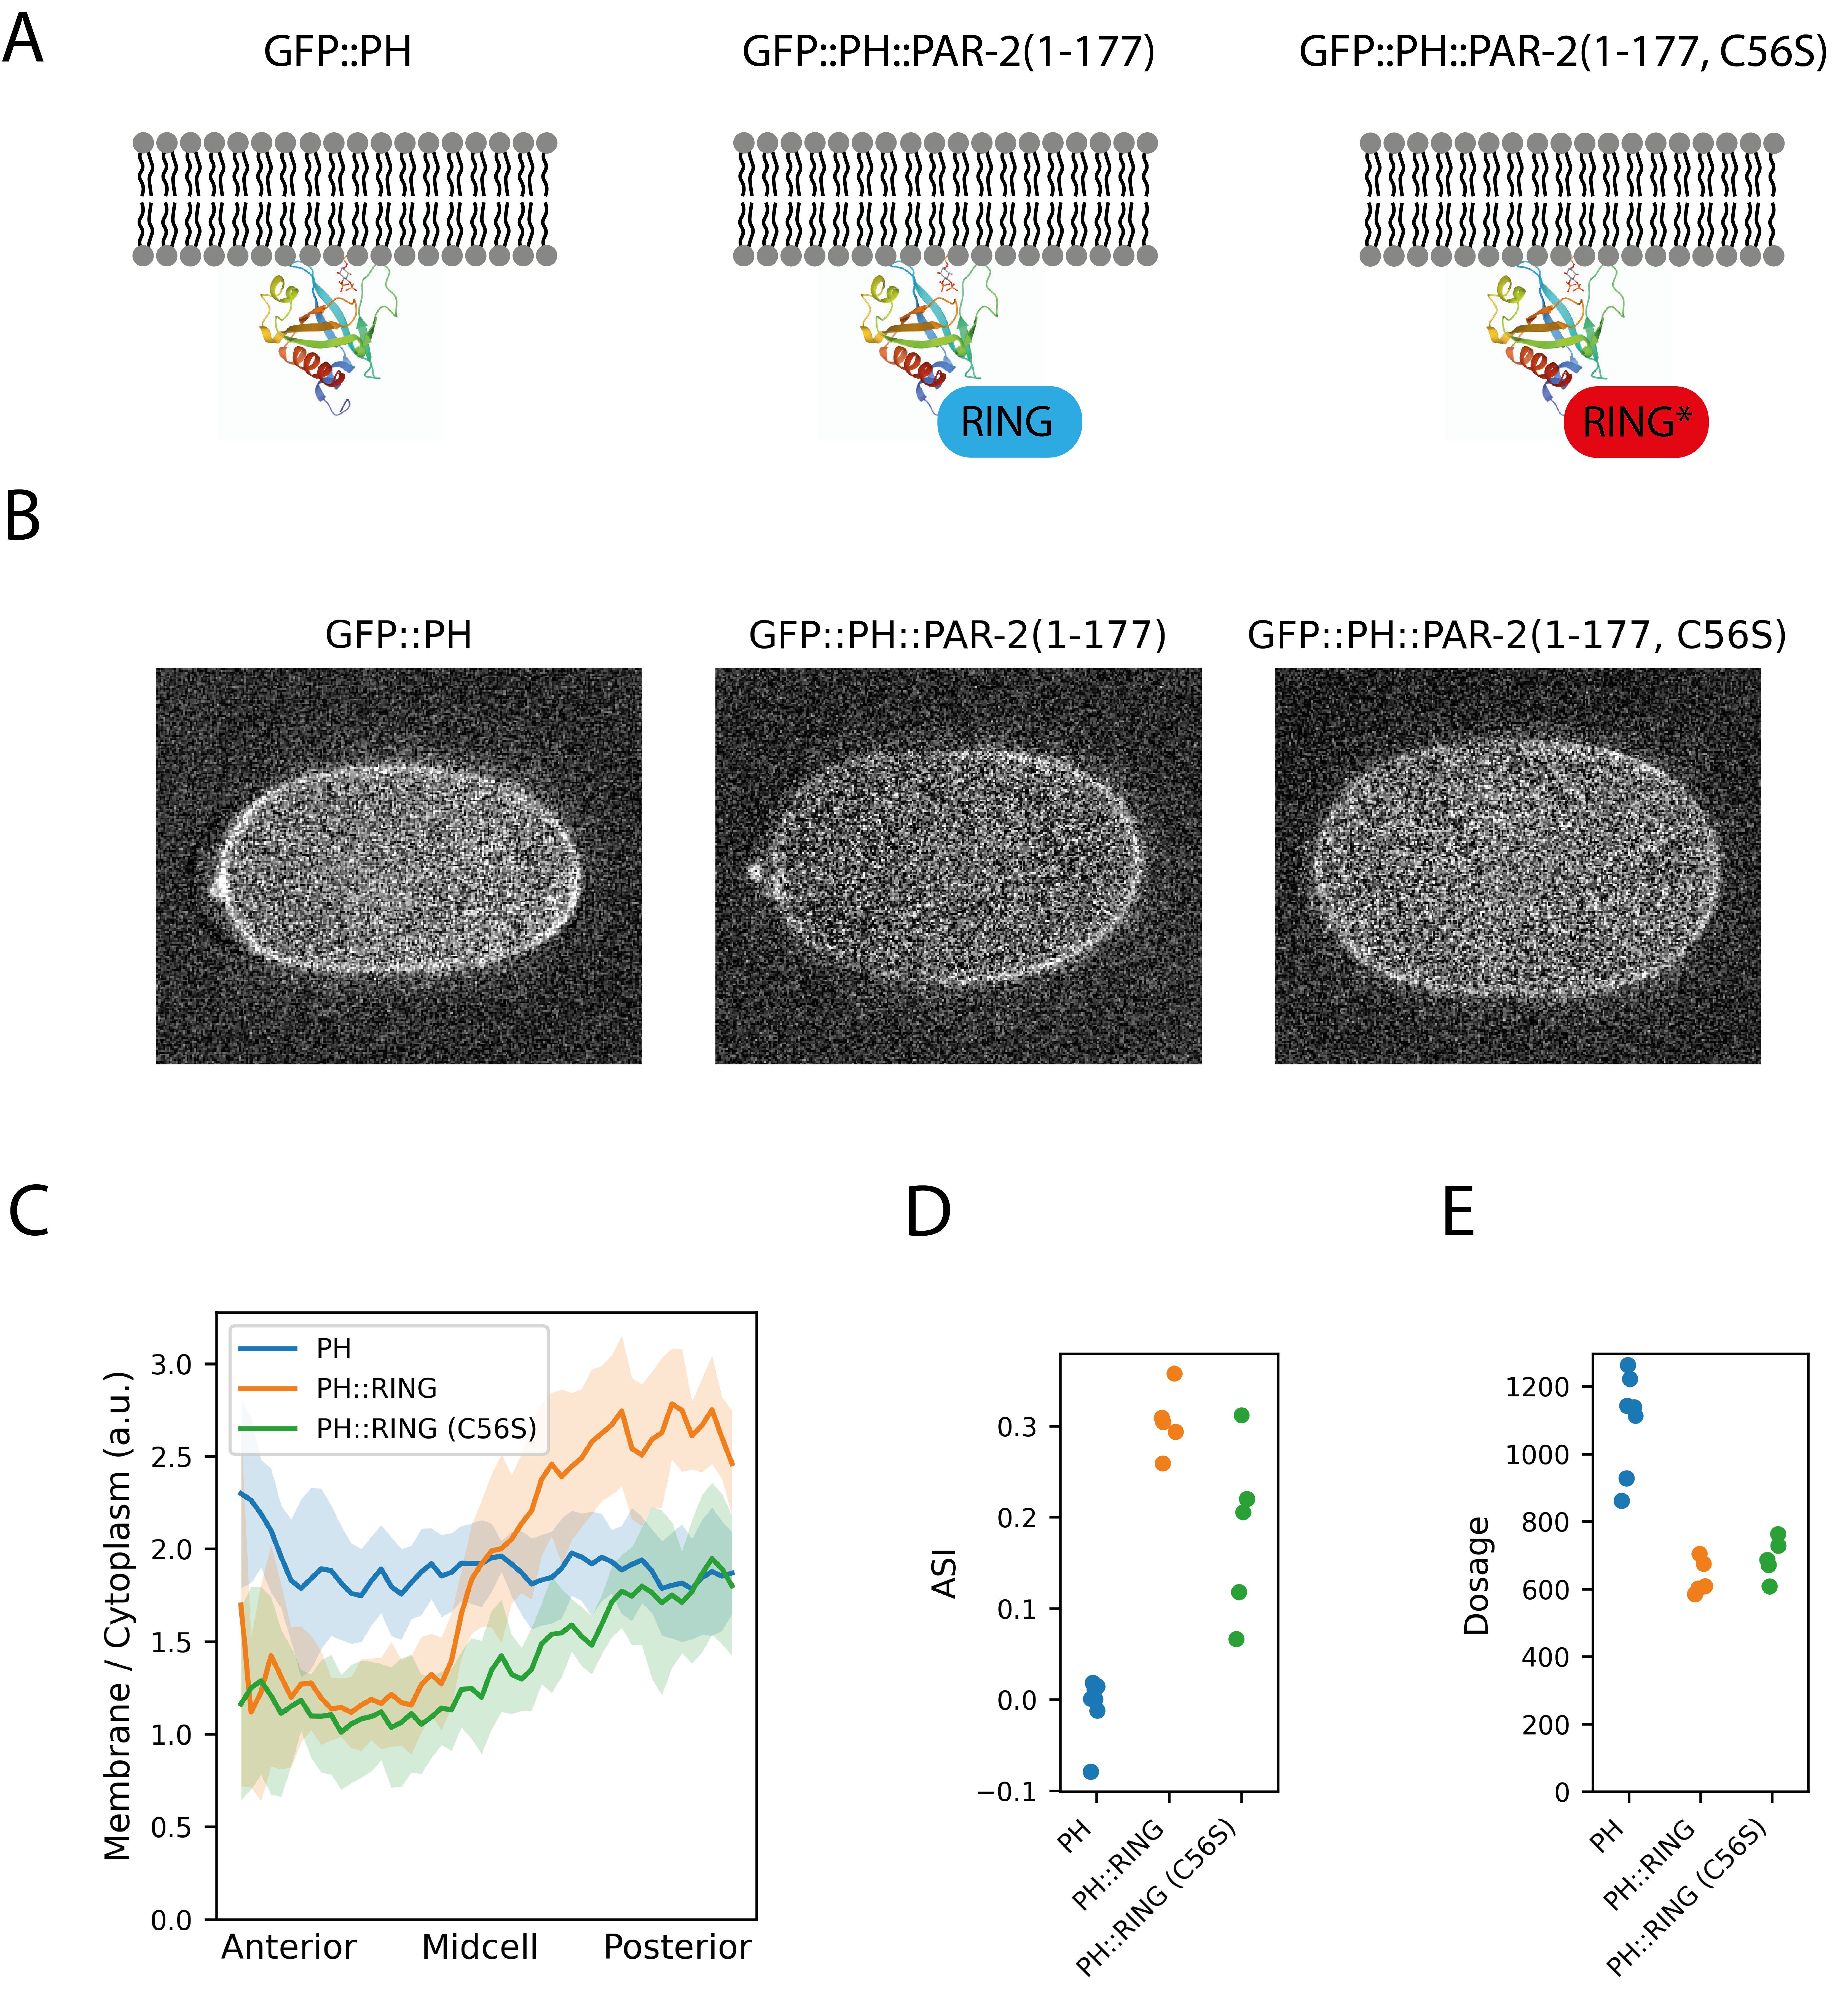
\includegraphics[scale=1]{ph_ring}
\setlength{\abovecaptionskip}{20pt}
\centering
\mycaption{Membrane-tethered RING domain fragment drives posterior localisation}{
\textbf{(A)} Schematic of the three constructs tested (GFP not shown).
\textbf{(B)} Midplane confocal images of the three constructs.
\textbf{(C)} Quantification of membrane to cytoplasmic ratios for the three constructs (Mean $\pm$ SD).
\textbf{(D)} Quantification of asymmetry index using the data in (C).
\textbf{(E)} Total expression of the three constructs. Expression of GFP::PH was downregulated by RNAi, aiming to roughly match expression of the other two constructs.
}
\label{fig:ph_ring}
\end{figure}

\begin{figure}
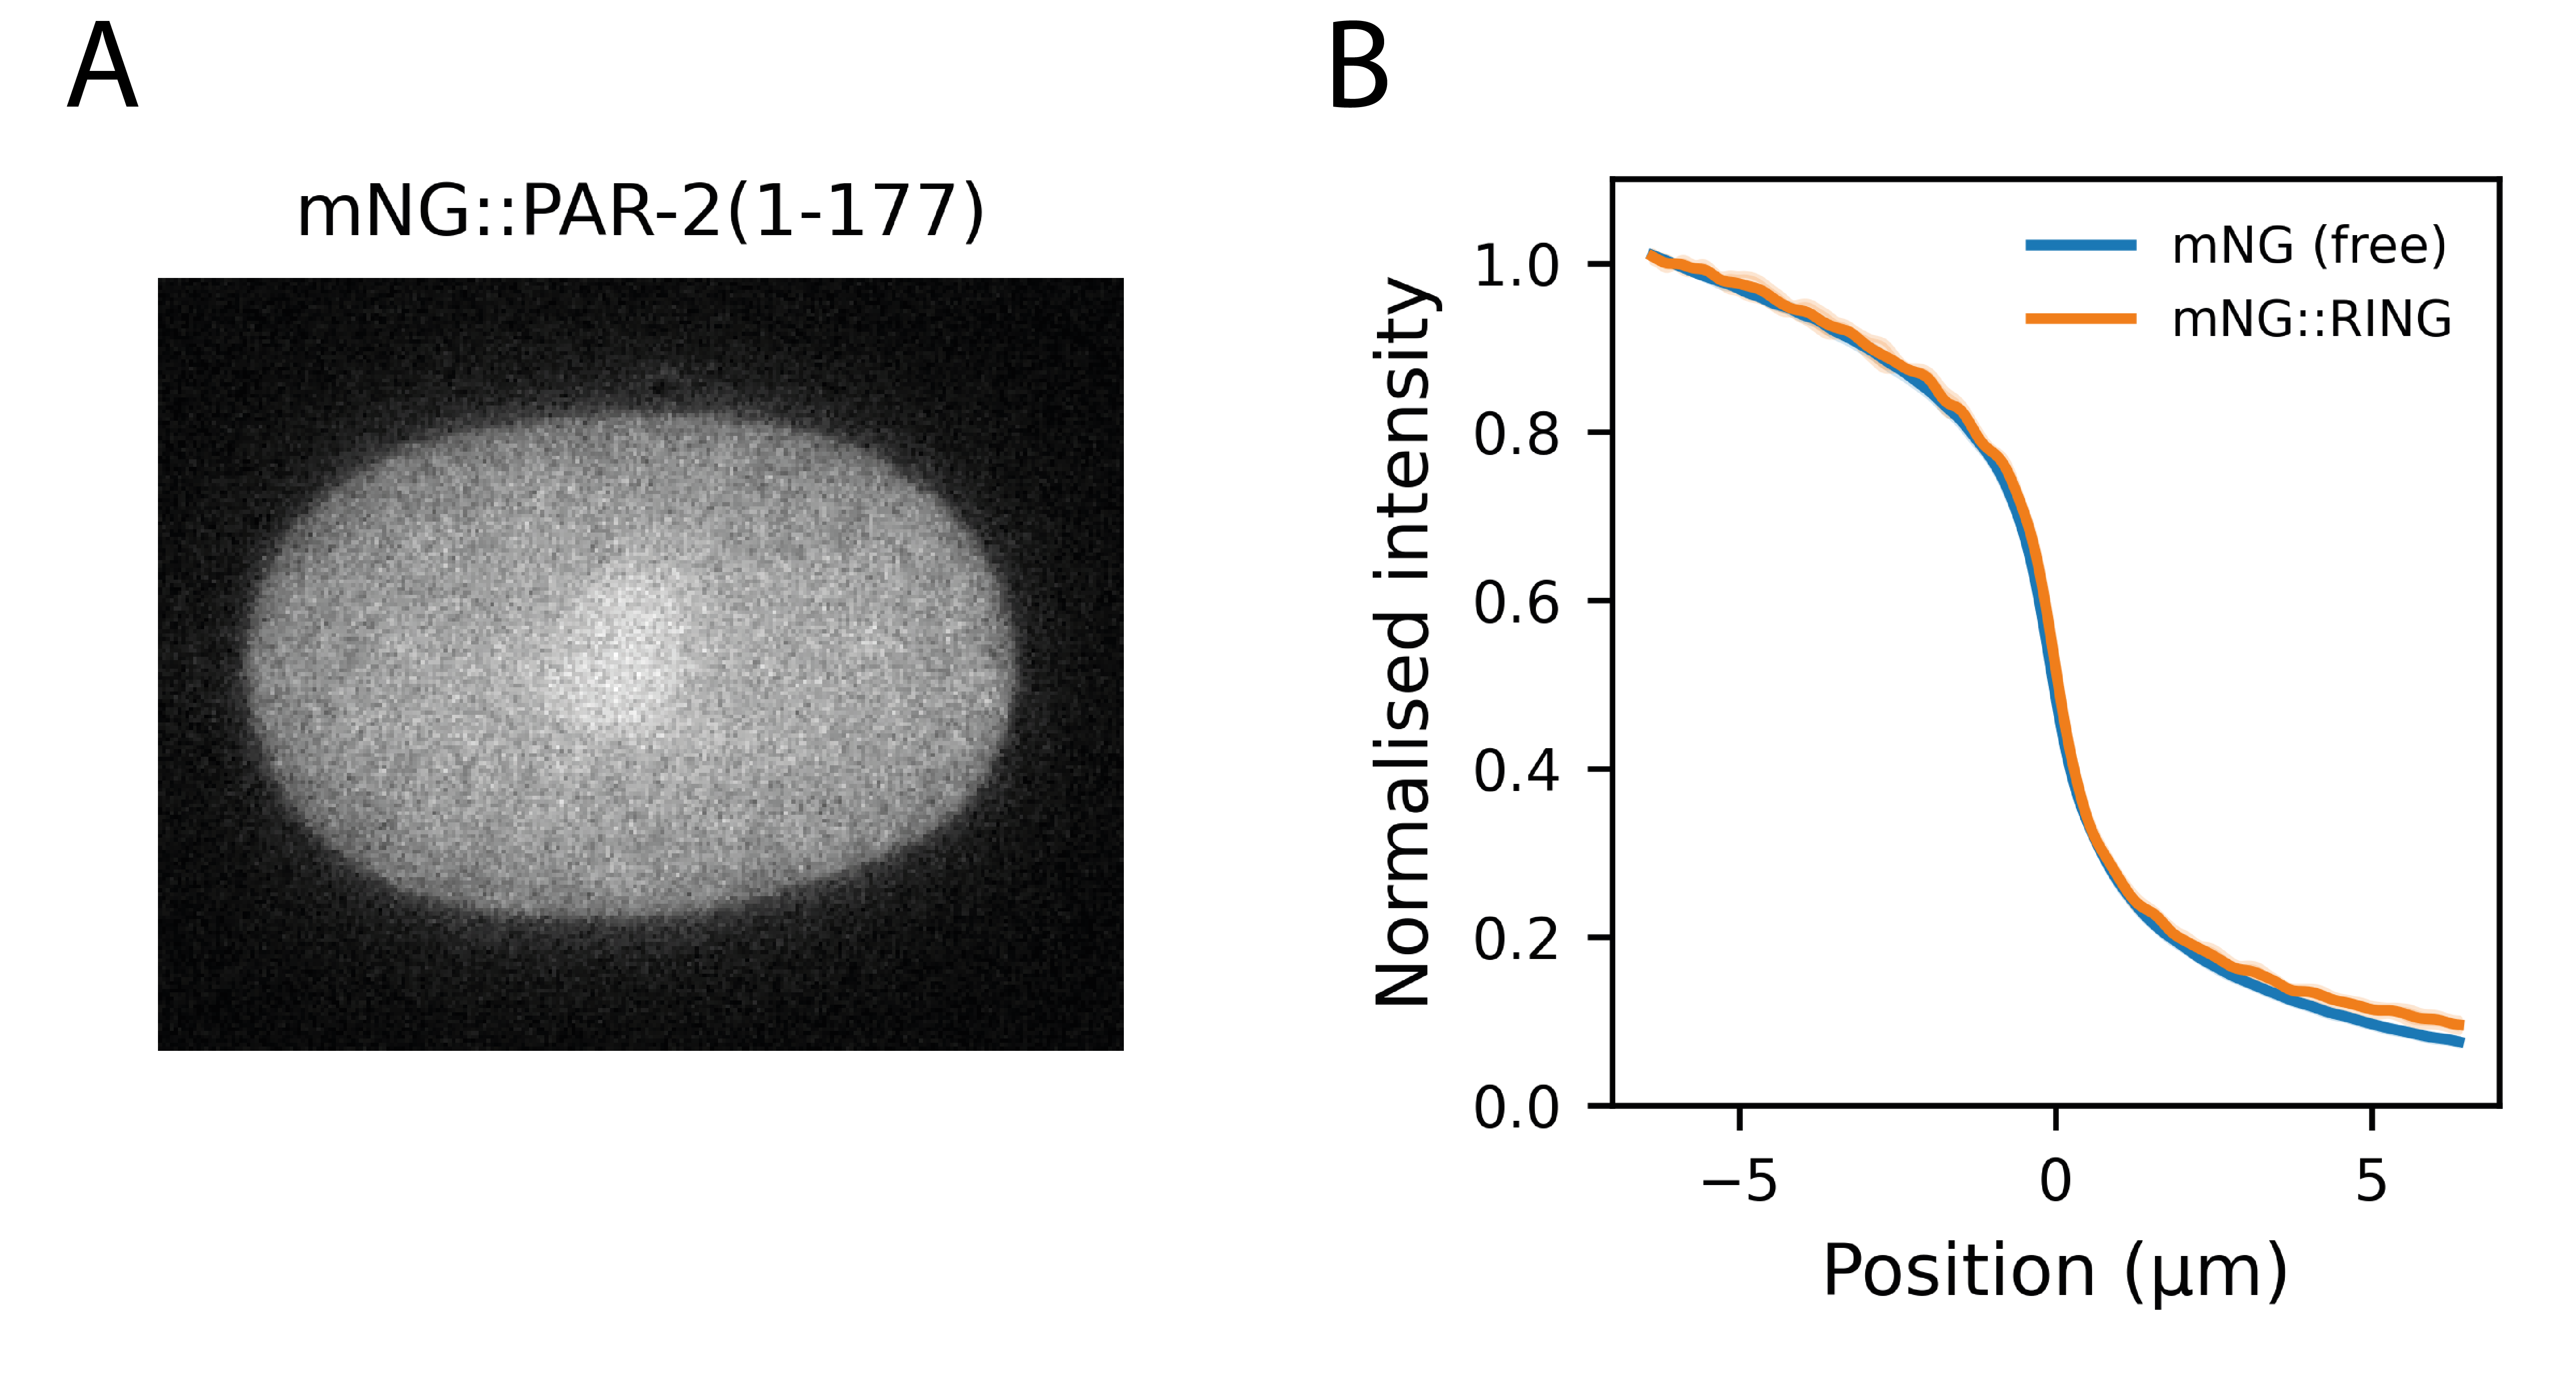
\includegraphics[scale=1]{ring_fragment_in_vivo}
\centering
\mycaption{PAR-2 RING domain fragment shows no membrane localisation}{
\textbf{(A)} Midplane image of mNG::PAR-2(1-177), showing entirely cytoplasmic localisation.
\textbf{(B)} Normalised cross-cortex profile of mNG::PAR-2(1-177) compared to mNG alone.
}
\label{fig:ring_fragment_in_vivo}
\end{figure}

These results imply that the GFP::PH::RING construct is polarising by dimerising with polarised endogenous PAR-2. Therefore, it is expected that disrupting polarity of endogenous PAR-2 should disrupt this localisation. To test this, I disrupted endogenous polarity using RNAi against \textit{par-2} or \textit{par-6}, and visualised the effect on the GFP::PH::RING construct (\cref{fig:ph_ring_rnai}). In conditions of \textit{par-2} RNAi, endogenous PAR-2 is expected to be entirely absent from the cell, and aPARs mostly uniform. Under these conditions, the construct loses enrichment in the posterior, and overall polarity is low. Similarly, in conditions of \textit{par-6} RNAi, where endogenous PAR-2 is expected to be uniform on the membrane, albeit less weakly concentrated, the construct also loses the ability to enrich in the posterior. Whilst we might expect overall affinity to be higher in the \textit{par-6} RNAi condition, as there is some level of endogenous PAR-2 on the membrane, this doesn't appear to be the case in this assay. This may imply a concentration dependent effect, whereby the construct is only able to respond to endogenous PAR-2 that's highly concentrated on the membrane.\\

\begin{figure}
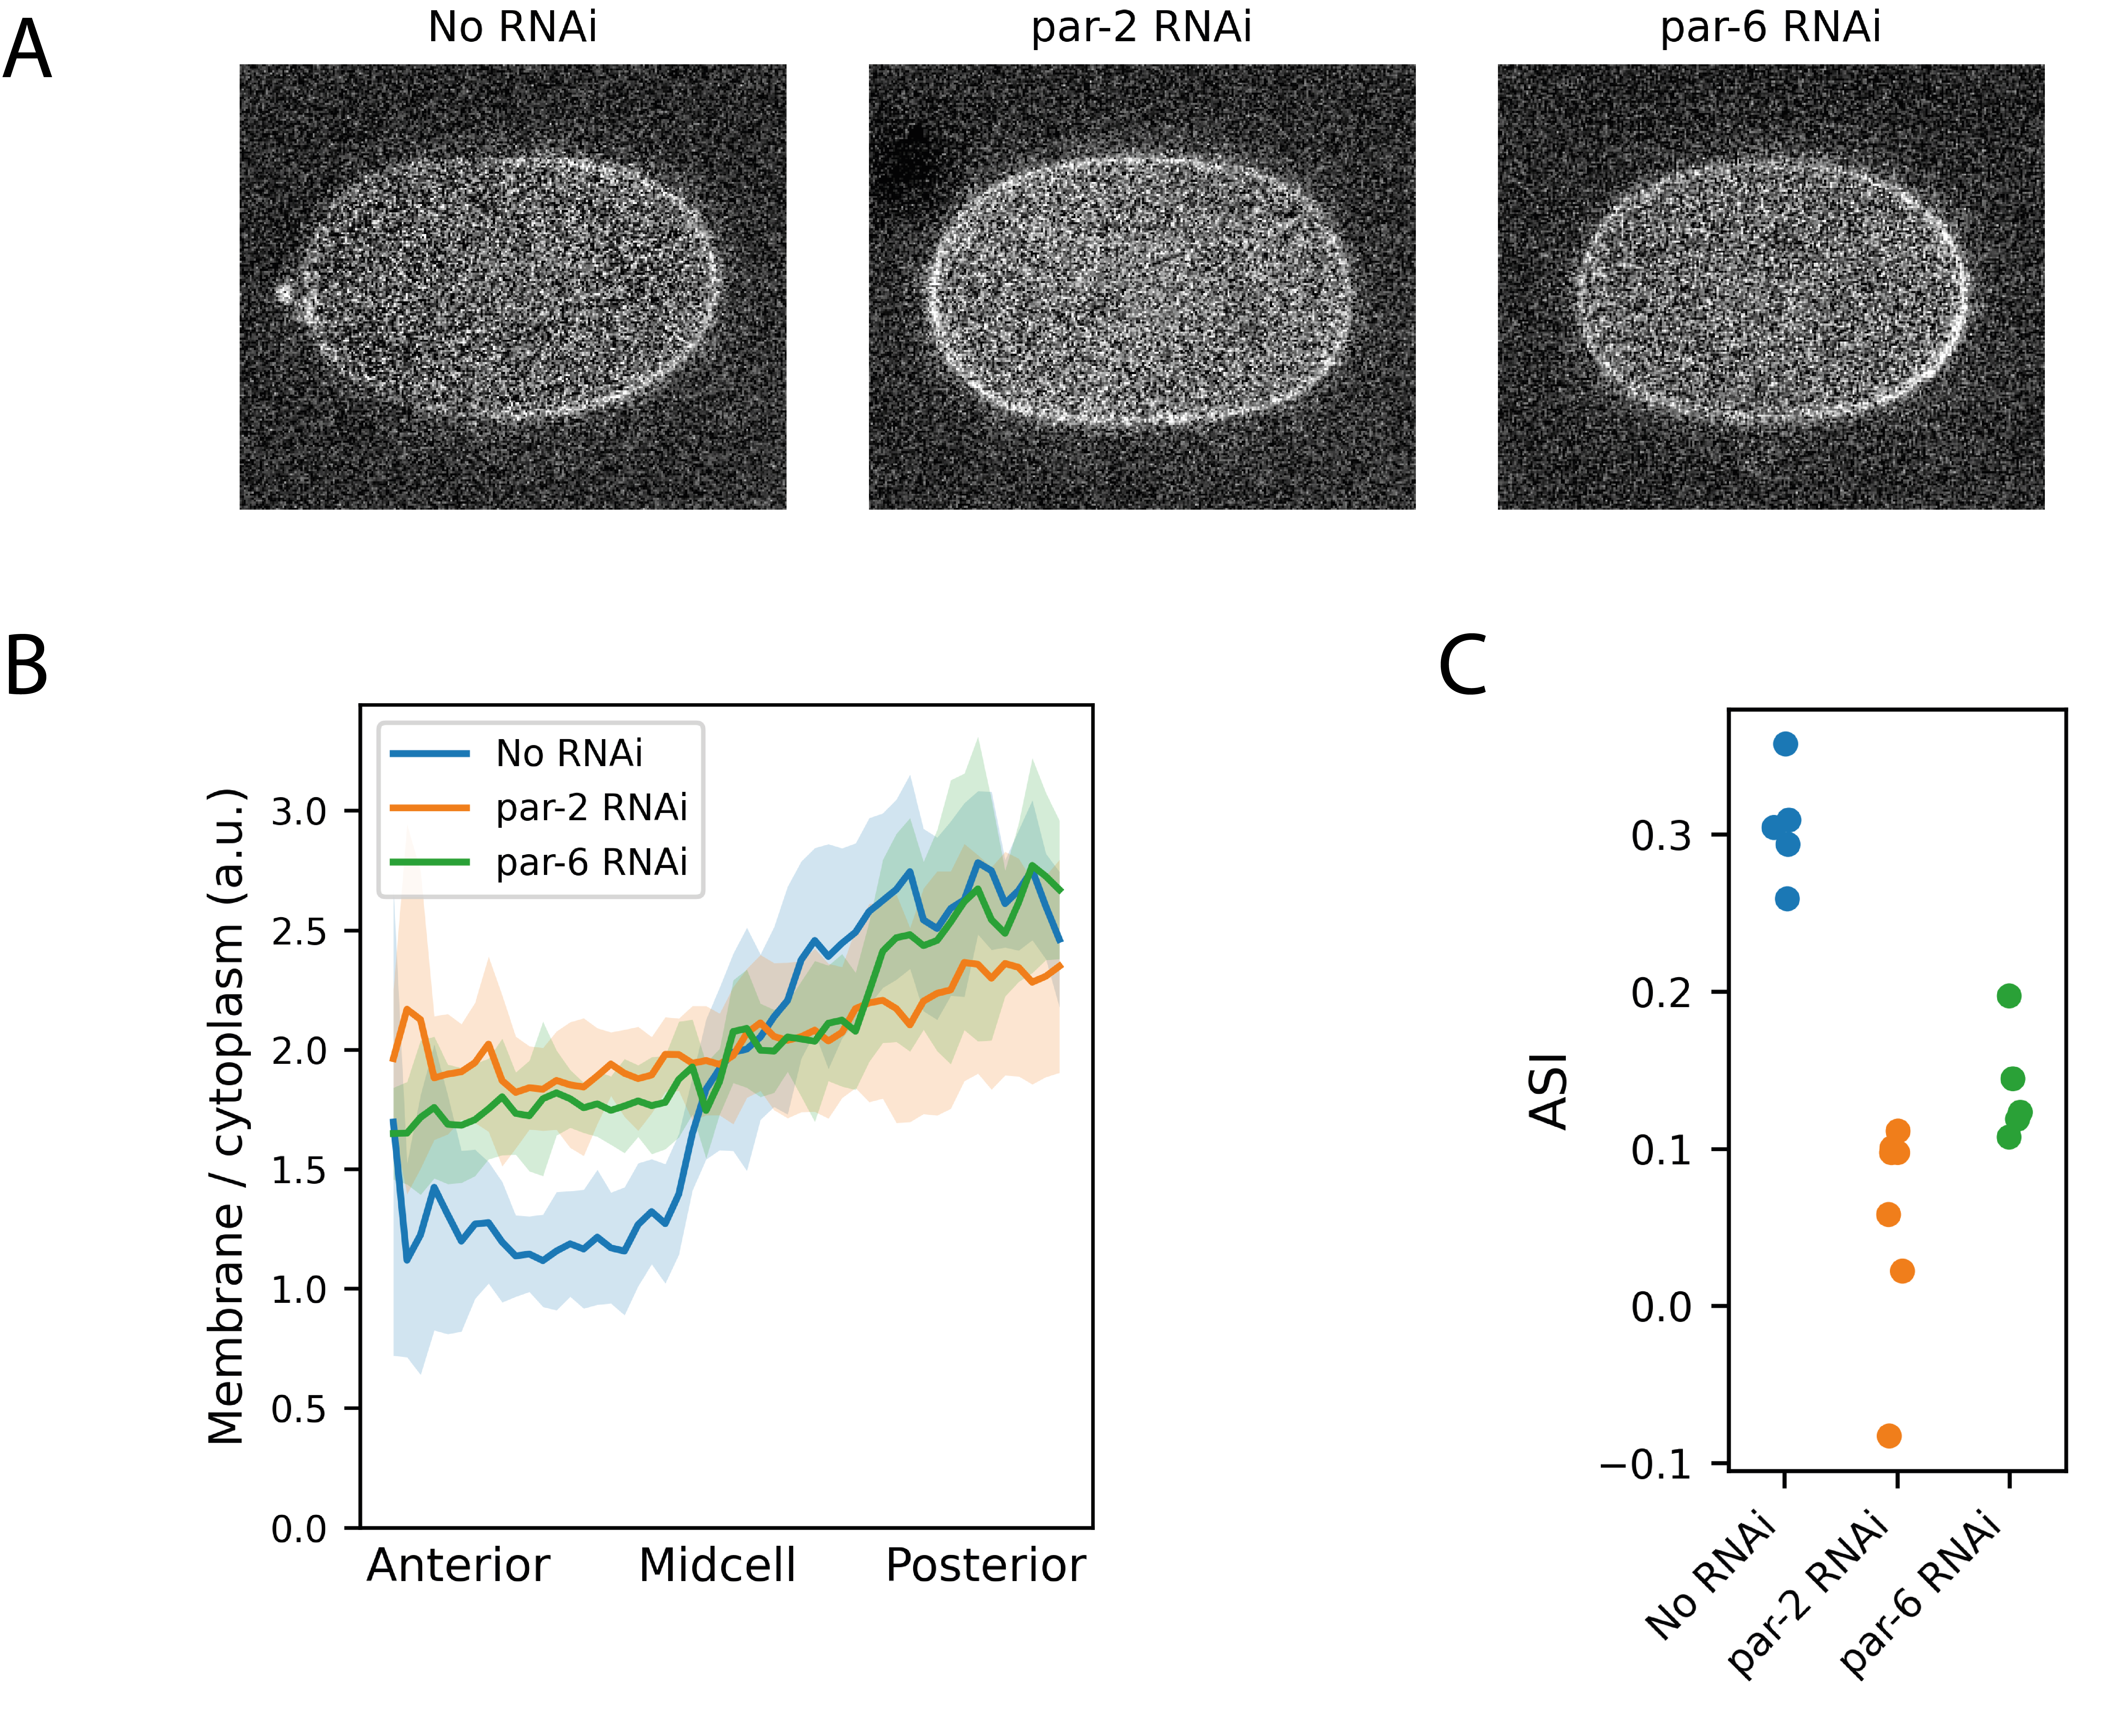
\includegraphics[scale=1]{ph_ring_rnai}
\centering
\mycaption{Localisation of membrane-tethered RING domain is dependent on endogenous PAR patterns}{
\textbf{(A)} Midplane confocal images of GFP::PH::RING under conditions of no RNAi, \textit{par-2} RNAi and \textit{par-6} RNAi.
\textbf{(B)} Quantification of membrane to cytoplasmic ratios for the three constructs (Mean $\pm$ SD).
\textbf{(C)} Quantification of asymmetry index using the data in (C).
}
\label{fig:ph_ring_rnai}
\end{figure}


\subsection{Mutation to dimerisation interface weakens membrane association in vivo}

Overall, the data described so far suggests a mechanism whereby cytoplasmic PAR-2 is monomeric, and enrichment on the membrane switches PAR-2 to a dimeric state via a concentration-dependent dimerisation reaction. I next aimed to investigate the potential importance of this dimerisation reaction in vivo. As discussed previously, unfolding the RING domain by targeted mutation to a zinc-interacting cysteine has a strong phenotype in vivo, characterised by a strong reduction in membrane affinity. However, as C56S mutation is expected to disrupt the tertiary structure of the whole domain, rather than just the dimerisation interface, it may also have additional effects. Structure prediction analysis and SEC-MALS data indicate that a single mutation to a hydrophobic residue in the putative dimerisation interface (L109R) is sufficient to specifically disrupt dimerisation. To investigate the significance of PAR-2 dimerisation in vivo, I performed targeted mutations to this site by CRISPR in an mNG::PAR-2 background. In addition to L109R, I performed an additional L to R mutation to L50, which is found in the putative N-helix, and doesn't interact with L109 (\cref{fig:l50_structure}).\\

\begin{SCfigure}
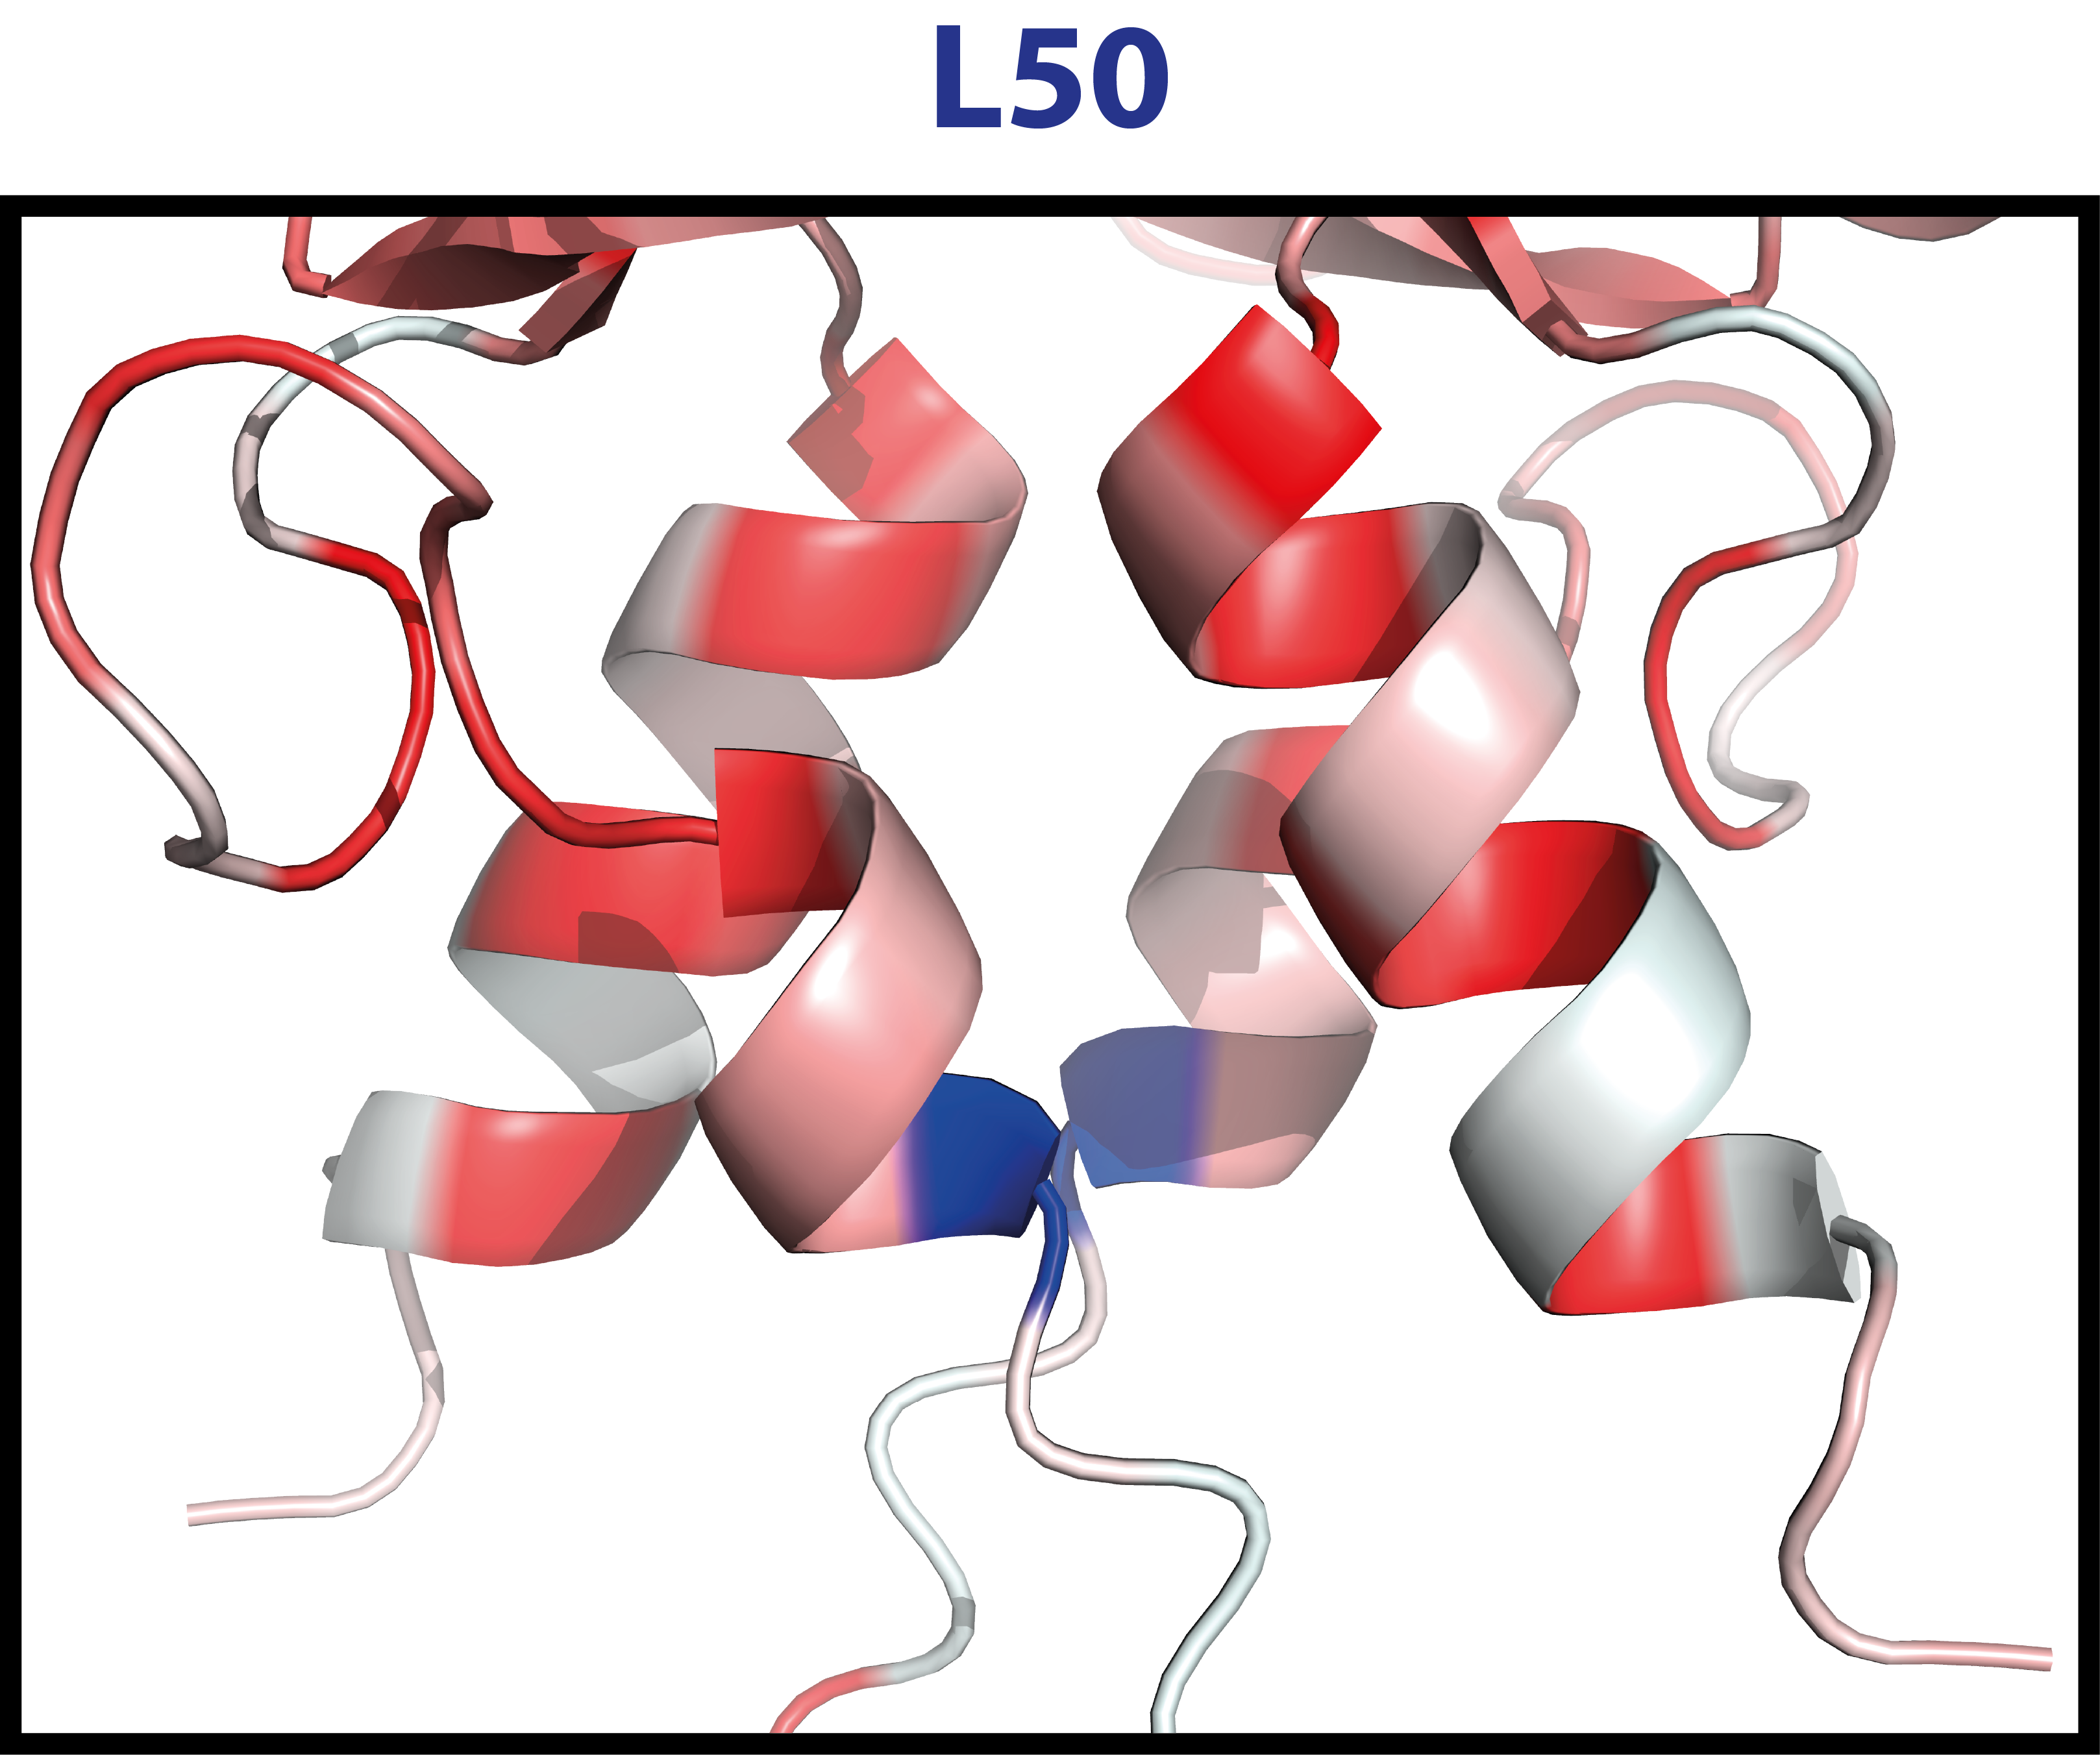
\includegraphics[scale=0.8]{l50_structure}
\mycaption{Position of the L50 site within the 4-helix bundle of the PAR-2 RING domain}{L50 site highlighted in blue, other residues coloured by hydrophobicity}
\label{fig:l50_structure}
\end{SCfigure}

As shown in \cref{fig:dimer_interface_mutants_in_vivo}, both mutations cause a strong reduction in membrane affinity. The effect is stronger for L109R than L50R, which may suggest that L50R has a weaker disruptive effect on dimerisation. Combining both mutants has no effect compared to L109R alone, which implies that dimerisation is completely disrupted in L109R. Interestingly, however, neither mutant reduces membrane affinity to the same extent as C56S. Assuming that dimerisation is fully disrupted by L109R, this implies that fully unfolding the domain may have additional effects compared to just disrupting dimerisation alone. One plausible explanation is that, in the case of C56S, the unfolded domain interferes with normal membrane binding, and therefore has an additional negative effect on membrane affinity. Compatible with this, a PH::RING fusion has lower overall membrane affinity than PH alone (\cref{fig:ph_ring}). Combining C56S and L109R has no effect compared to C56S alone, suggesting that dimerisation is completely disrupted in the C56S mutant.\\

\begin{figure}
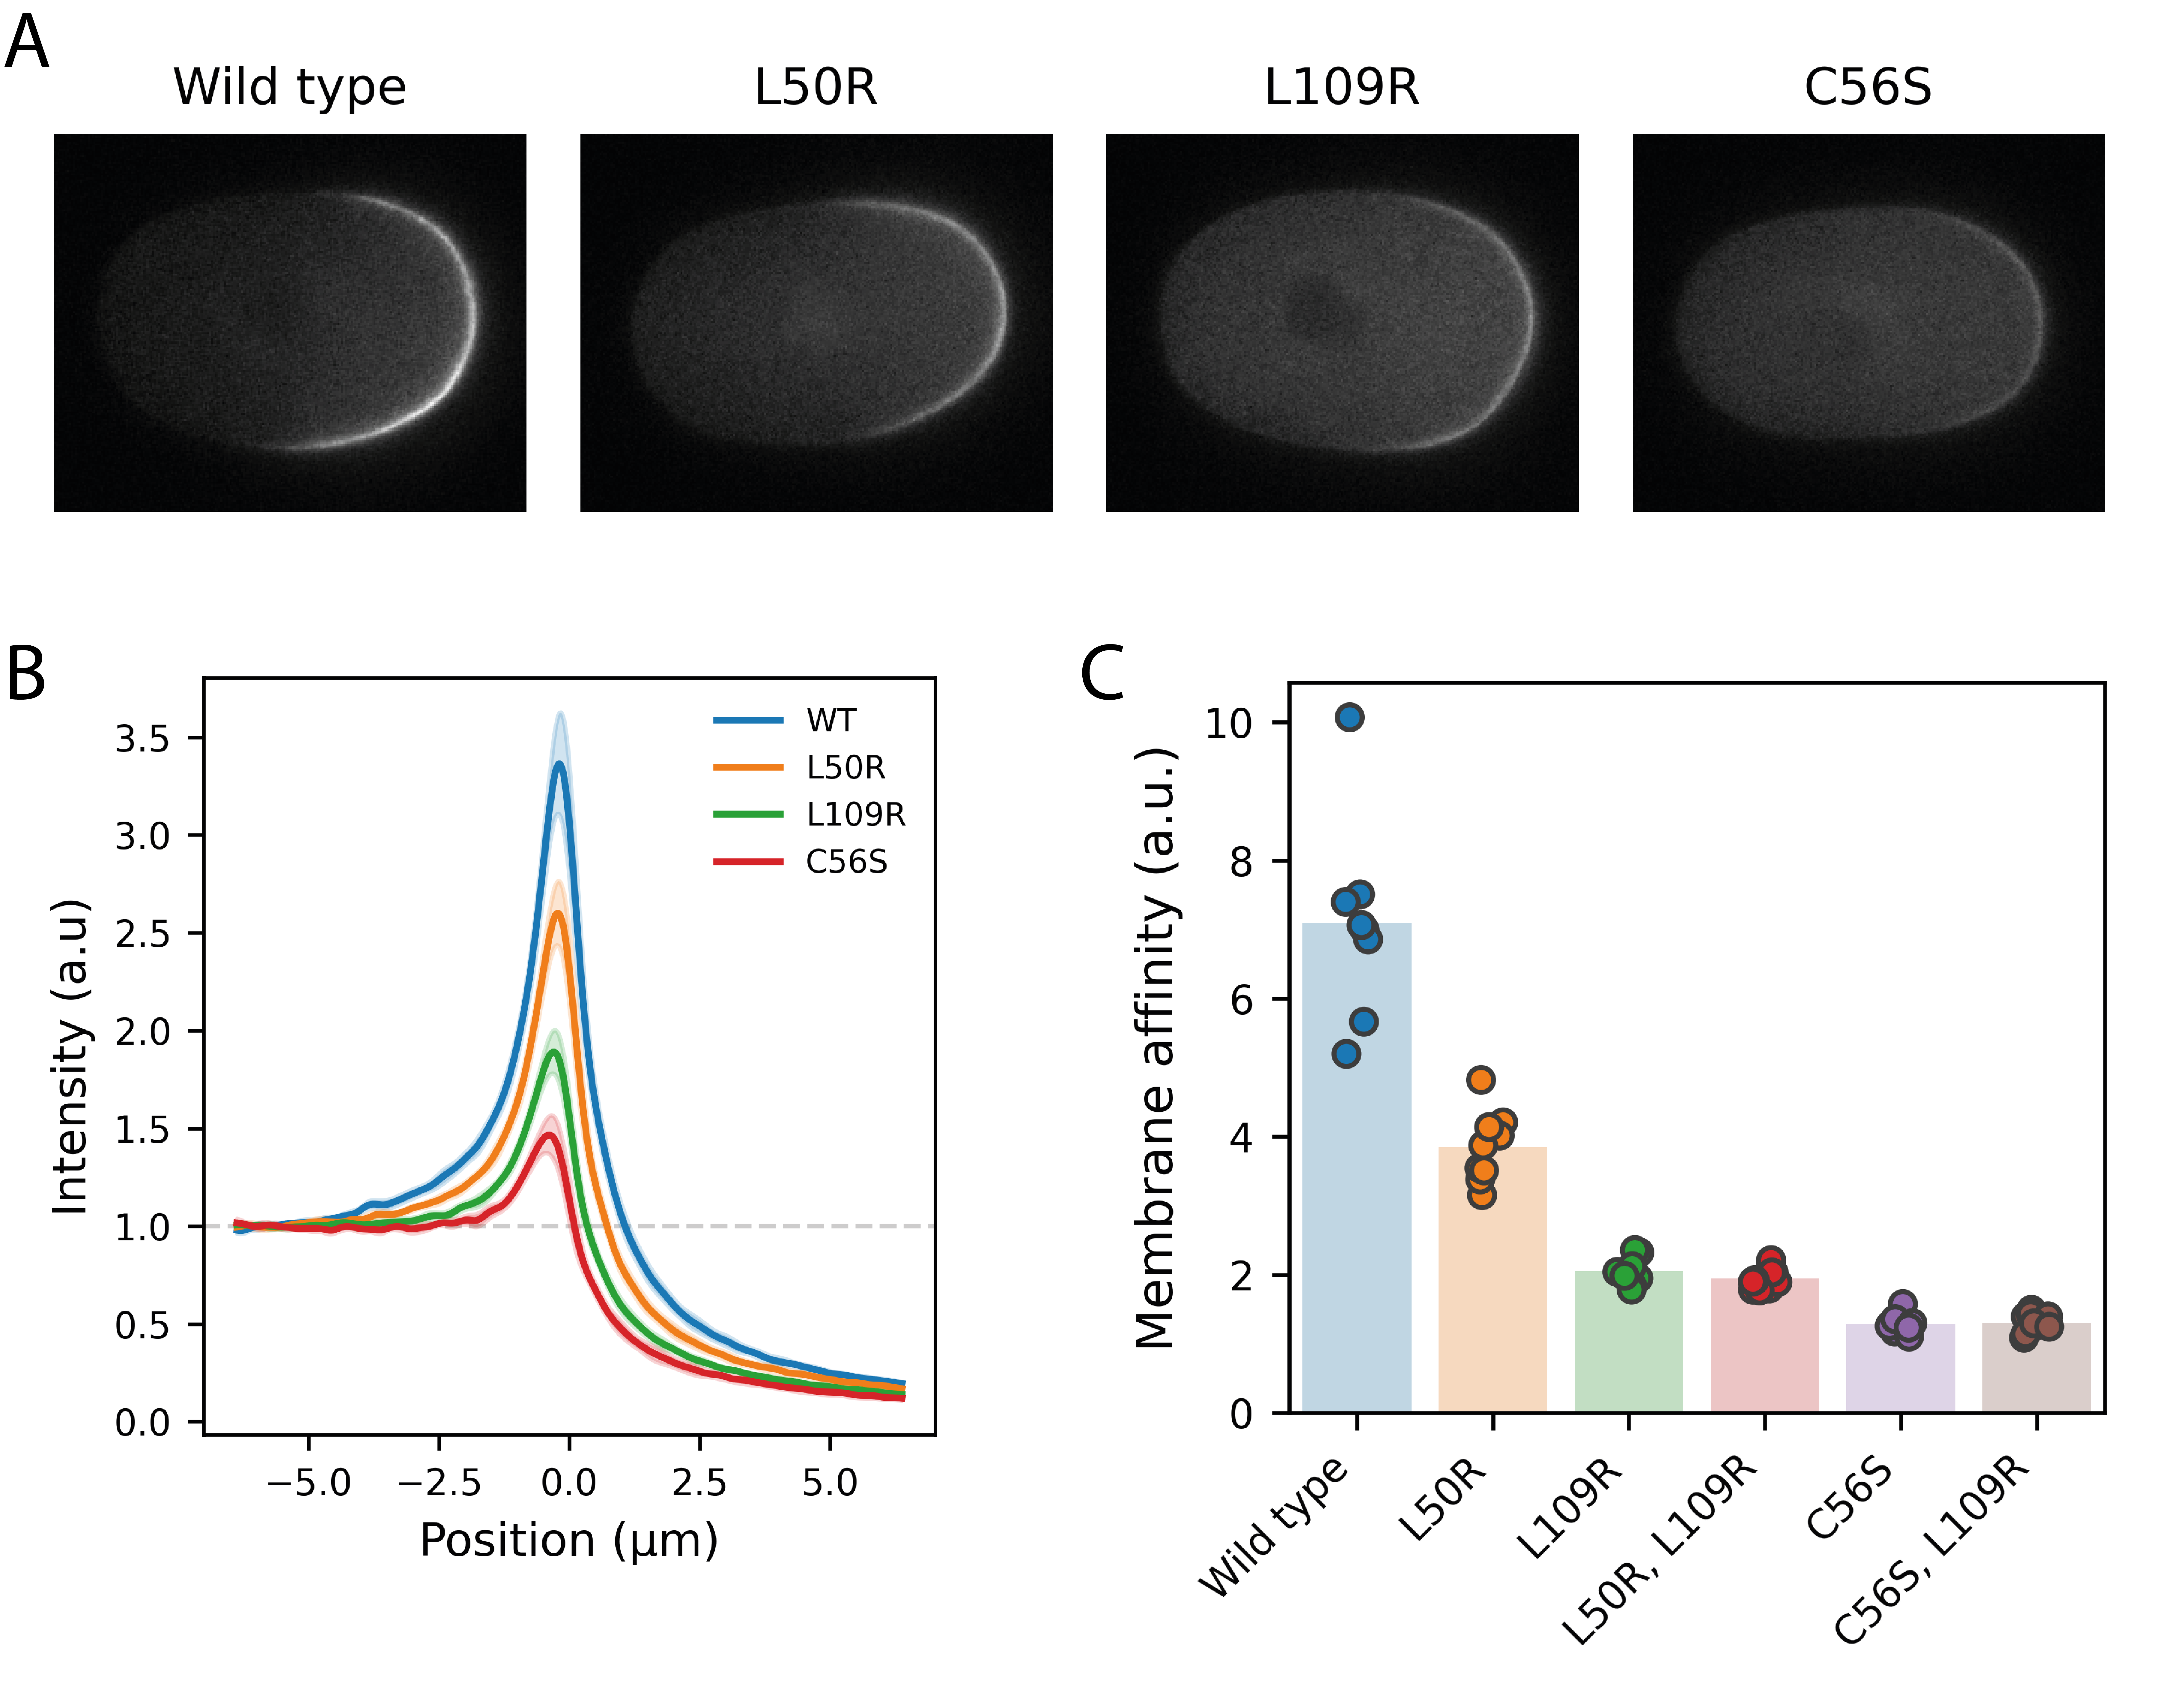
\includegraphics[scale=0.9]{dimer_interface_mutants_in_vivo}
\centering
\mycaption{Dimerisation interface mutants disrupt PAR-2 membrane association}{
\textbf{(A)} Midplane confocal images of wild type, L50R, L109R and C56S PAR-2.
\textbf{(B)} Normalised cross-cortex profiles for the four PAR-2 alleles in (A).
\textbf{(C)} Quantification of membrane to cytoplasmic ratio for the four mutants and (A) and (B) and two additional combined mutants.
}
\label{fig:dimer_interface_mutants_in_vivo}
\end{figure}

To determine the effects of these mutants on organism development, I investigated levels of embryonic lethality and adult sterility (\cref{fig:ring_lines_lethality_sterility}). Interestingly, whilst C56S lines have high levels of lethality and sterility, this isn't the case for the dimerisation interface mutants. It may be that the additional loss of membrane affinity in C56S mutants has a significant impact on pPAR domain integrity, which may be important in later developmental stages as well as in the zygote. Even though no effects were observed for L50R and L109R compared to wild type, it's likely that defects would be observed in non wild-type backgrounds (e.g. LGL-1 mutant), or with reduced PAR-2 expression (e.g. heterozygous). This remains to be investigated.\\

\begin{figure}
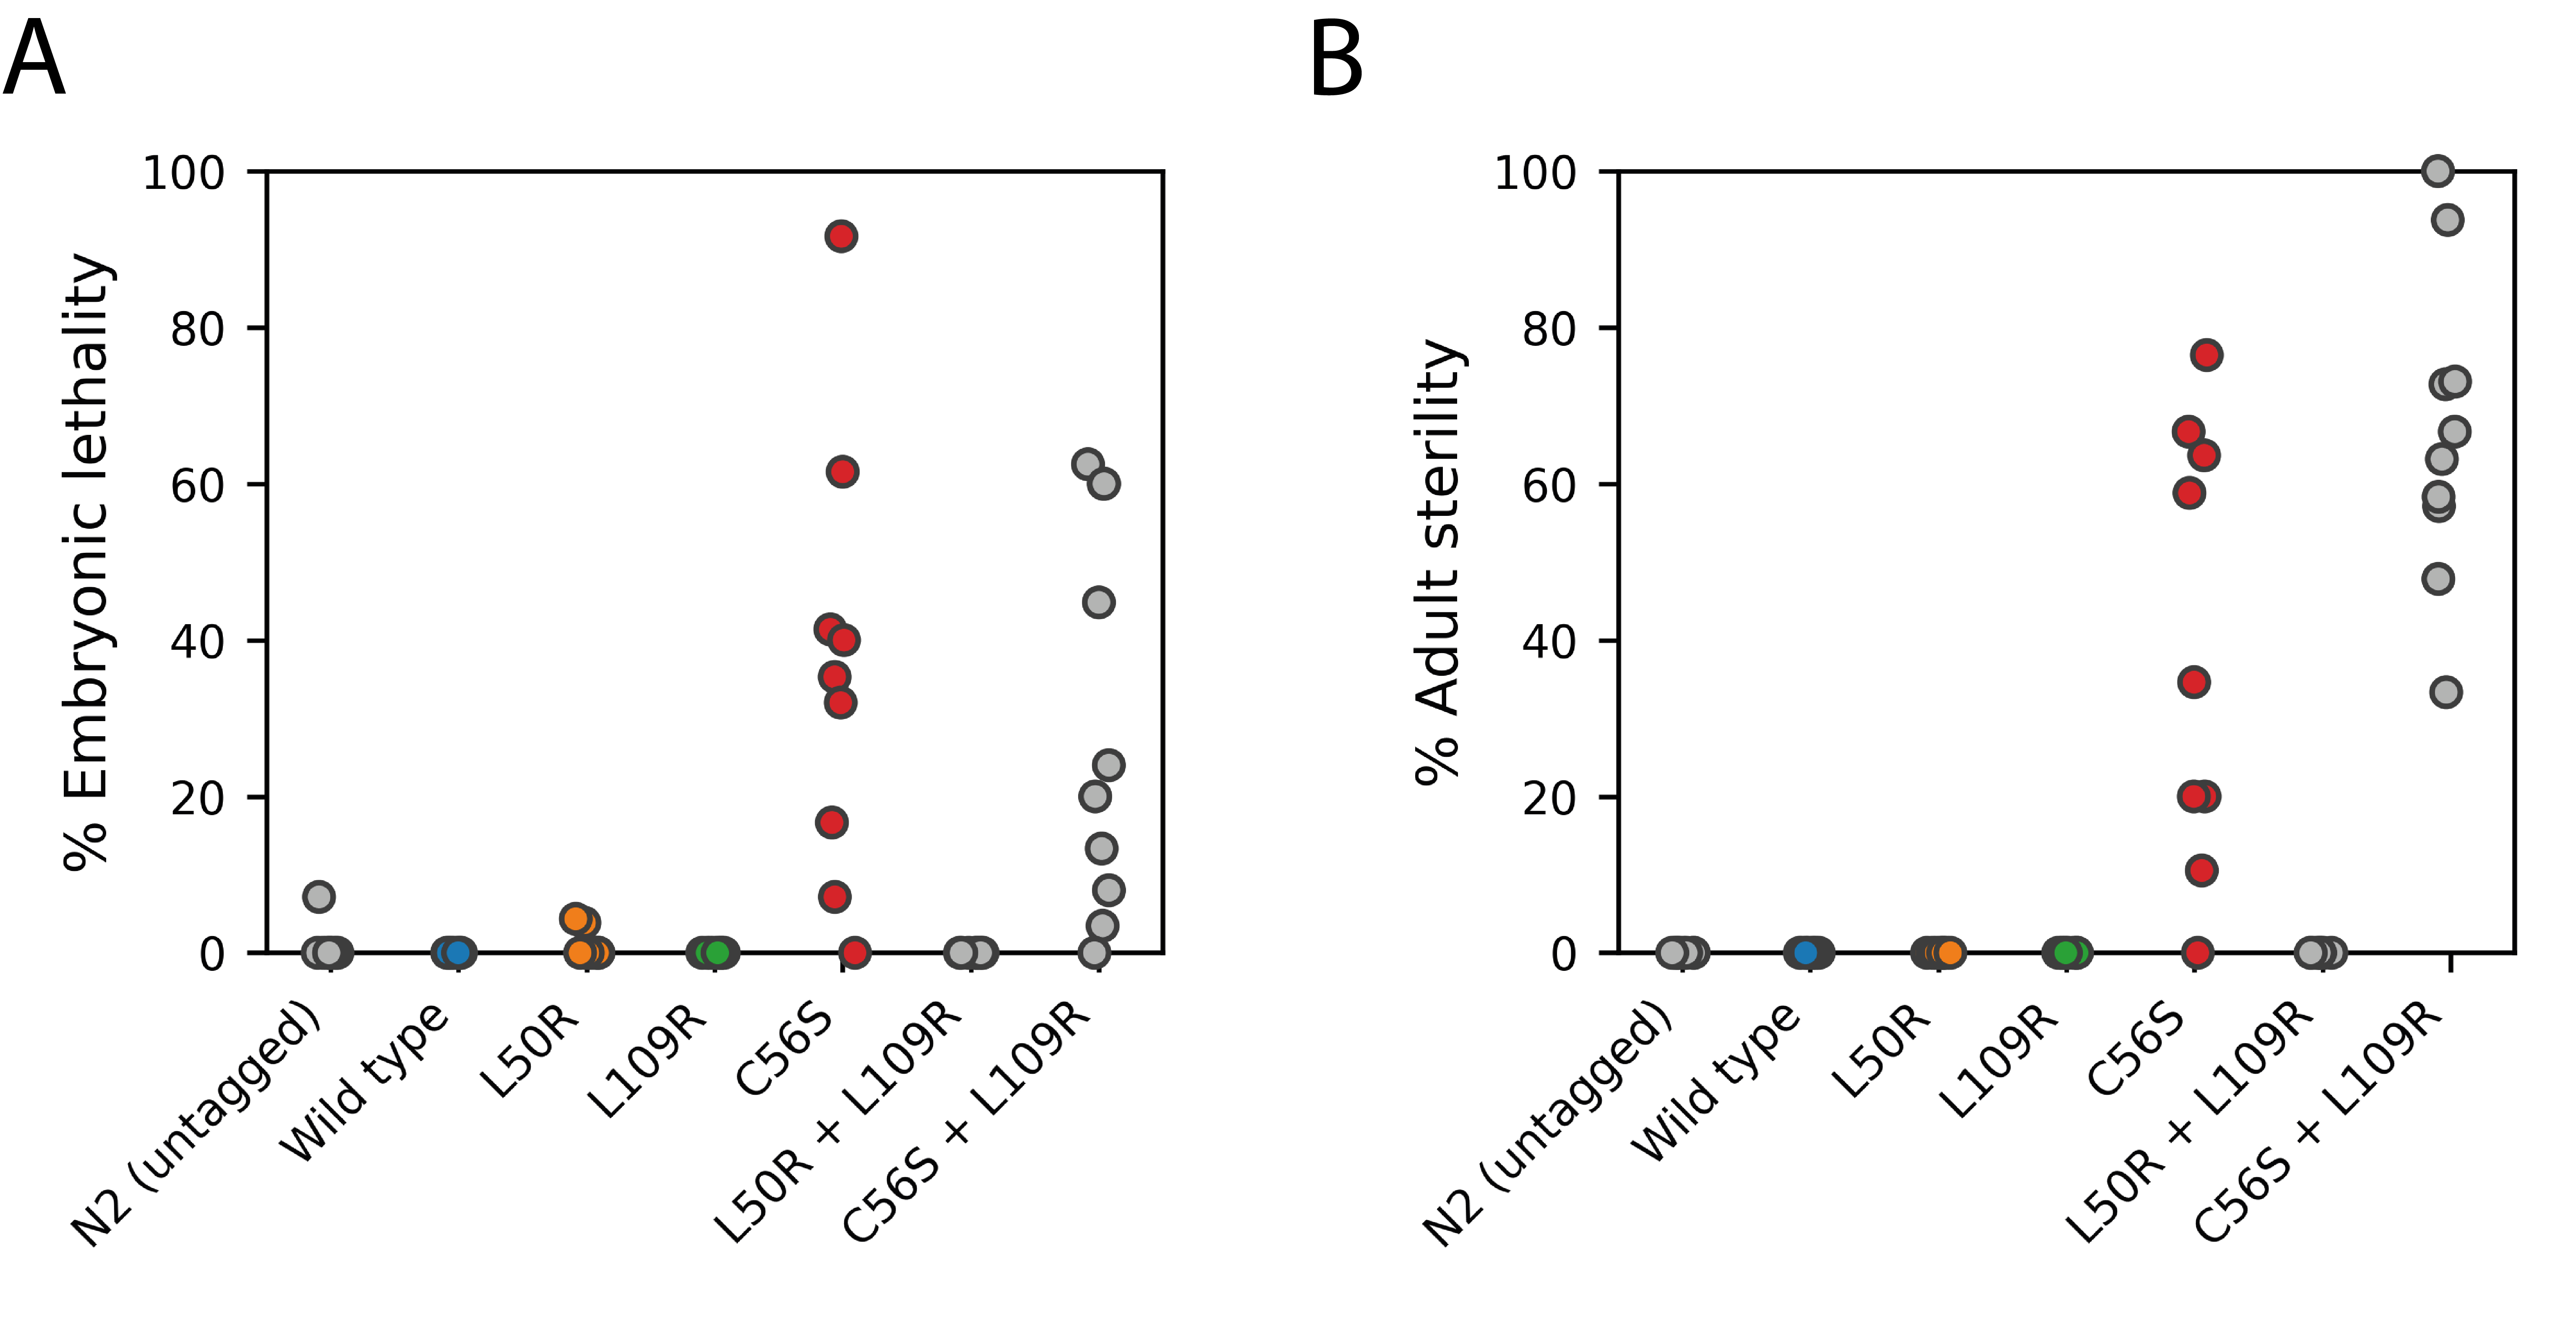
\includegraphics[scale=1]{ring_lines_lethality_sterility}
\centering
\mycaption{Embryonic lethality and adult sterility in RING mutant lines}{
\textbf{(A)} Percentage embryonic lethality. Individual points represent the percentage of dead embryos laid by one gravid adult worm over a period of 5 hours at room temperature.
\textbf{(B)} Percentage adult sterility. Individual points represent the percentage of sterile worms in the total progeny of one adult worm 48 hours after egg laying.
}
\label{fig:ring_lines_lethality_sterility}
\end{figure}


\subsection{Discussion}

% comment on arata paper

% Plausibly, if autoubiquitination does play a role, and this is dimerisation dependent, then dimerisation interface mutants could would also work through this mechanism.


%%%%%%%%%%%%%%%%%%%%%%%%%%%%%%%%%%%%%%%%%%%%%%%%%%%%%%%%%%
\clearpage
\chapter{Modelling the interplay between dimerisation and membrane association}

\textbf{Detailed contributions:}\\
The thermodynamic model described in section \ref{section:thermodynamic_full_model} was developed by David Zwicker at the Max Planck Institute for Dynamics and Self-Organisation in G{\"o}ttingen, Germany. All the analysis presented in this chapter was performed by myself.\\

\clearpage
\section*{Symbols}

I will use the following symbols throughout the chapter to describe to the chemical properties of an equilibrium system:\\

\begin{tabular}{ll}
$G$ & total Gibbs energy of the system\\
$G_x$ & Gibbs energy of a system of pure $x$\\
$n_x$ & number of moles of $x$\\
$\mu_x$ & chemical potential of $x$\\
$\mu_x^{\circ}$ & standard chemical potential of $x$\\
$c_x$ & molar concentration of $x$\\
$c^{\circ}$ & standard concentration\\
$R$ & the gas constant\\
$T$ & temperature in kelvins
\end{tabular}


\clearpage
\section{Introduction}

In the previous chapter, I showed that the RING domain of PAR-2 can dimerise, and that membrane bound PAR-2 is, at least partially, dimeric. I also showed that a series of RING domain mutants have a lower membrane affinity, suggesting that dimerisation may be fundamental for achieving high membrane affinity. Added to this, I have shown that wild type PAR-2 displays nonlinear membrane binding association, which is disrupted in RING domain mutants. This suggests that dimerisation may lead to a form of feedback, whereby membrane affinity is enhanced as protein concentrations increase.\\

In this chapter, I investigate the potential link between these characteristics, and, more generally, investigate the extent to which dimerisation can influence the membrane binding behaviour of a protein. To do so, I will use chemical thermodynamics to model dimerisation and membrane binding in an equilibrium system. I will begin this chapter by introducing the general modelling framework, and will then use this framework to describe a model which incorporates dimerisation and membrane association. I will then use this model to investigate the potential influence of dimerisation on membrane association, and compare this to in vivo data of PAR-2 membrane association. Specifically, I investigate the extent to which the nonlinearity of PAR-2 membrane association can be accounted for by protein dimerisation, and whether differences in the membrane association behaviour of wild type PAR-2 and RING domain mutants can be accounted for by disruption to dimerisation.\\

% Thermodynamic equilibrium puts constraints on the behaviour of a system, and allows us to accurately describe behaviour with a small number of easily interpretable parameters. 


\clearpage
\section{Modelling chemical equilibria}
\label{sec:modelling_chemical_equilibria}

In a chemical reaction, chemical equilibrium is a state in which reactants and products are present at concentrations that have no tendency to change over time. Consider a closed system in which material is exchanging between two states, \textbf{a} and \textbf{b}:
\begin{center}
\ce{\textbf{a} <=> \textbf{b}}
\end{center}

Provided there are no additional inputs, the system will eventually reach an equilibrium in which the rates of the forward and reverse reactions are equal, and concentrations have no tendency to change over time. Energetically speaking, this equilibrium is reached when the total Gibbs free energy of the system ($G$) is minimised. This minimum energy at equilibrium ($G_{min}$) will be lower than the energy of a system of either pure \textbf{a} ($G_a$) or pure \textbf{b} ($G_b$), and so, regardless of how the system is initiated, the system will eventually stabilise with a mixture of the two states (\cref{fig:gibbs_profile}).\\ 

\begin{SCfigure}
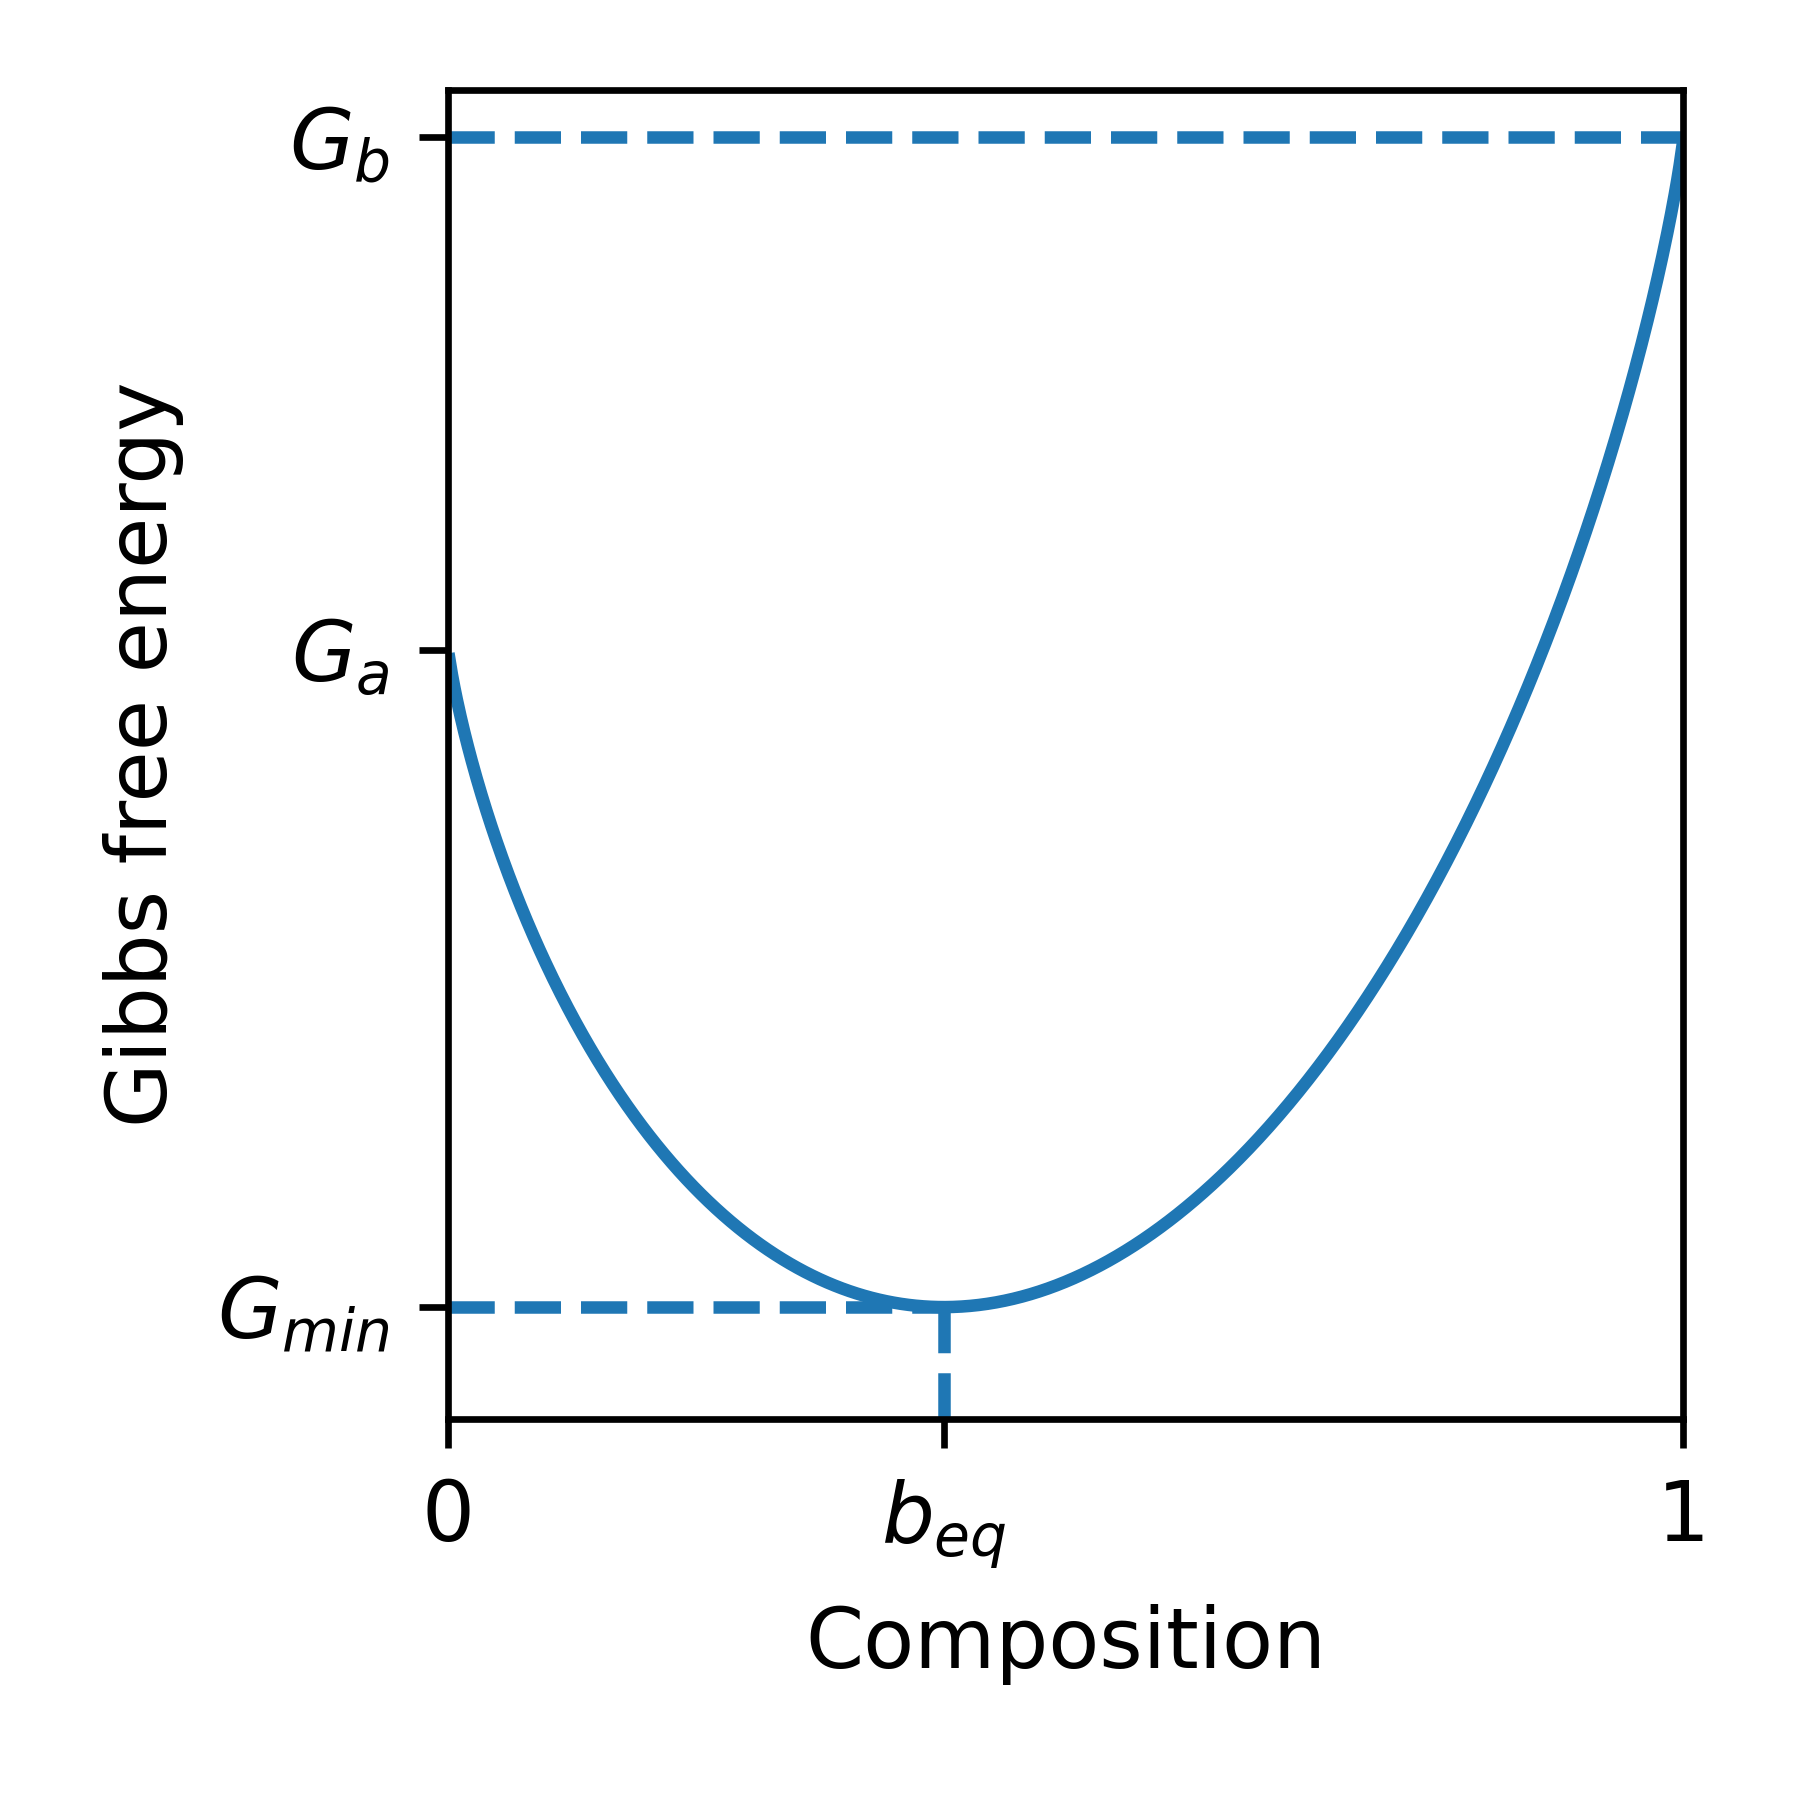
\includegraphics[scale=0.9]{gibbs_profile}
\mycaption{Gibbs energy profile for a system at equilibrium}{
Plot of the Gibbs energy of a system as a function of composition for a species converting between states \textbf{a} and \textbf{b} (where a composition of 0 means entirely in state \textbf{a} and 1 means entirely in state \textbf{b}). $G_a$ and $G_b$ represent the Gibbs energy of the system when all molecules are in state \textbf{a} or state \textbf{b}. The system reaches an equilibrium when $G$ is minimised ($G_{min}$), at which point the equilibrium concentration of \textbf{b} is $b_{eq}$ and \textbf{a} is (1 - $b_{eq}$).
}
\label{fig:gibbs_profile}
\end{SCfigure}

The position of equilibrium will depend on the intrinsic energetics of the two species. For example if $G_a$ is lower than $G_b$ (meaning that pure \textbf{a} is more energetically favourable than pure \textbf{b}), as is shown in \cref{fig:gibbs_profile}, the system will stabilise in a state with more \textbf{a} than \textbf{b}. Formally, we can describe $G$ according to the molar amounts of \textbf{a} and \textbf{b} ($n_a$ and $n_b$), and their associated chemical potentials ($\mu_a$ and $\mu_b$):
\begin{equation}
G = n_a \mu_a + n_b \mu_b
\label{eq:gibbs}
\end{equation}

Chemical potentials describe the Gibbs free energy density of each component in a mixture (i.e. energy per mole). These values vary with the molar concentration of each species ($c_a$ and $c_b$), and using ideal solution theory can be described as:
\begin{align}
\mu_a &= \mu_a^{\circ} + RT \ln \frac{c_a}{c^{\circ}}\\
\mu_b &= \mu_b^{\circ} + RT \ln \frac{c_b}{c^{\circ}}
\end{align} 

where $c^{\circ}$ is the standard concentration (usually defined as 1 mol dm$^{-3}$) and $\mu_a^{\circ}$ and $\mu_b^{\circ}$ are the standard chemical potentials of \textbf{a} and \textbf{b} (i.e. chemical potentials at the standard concentration). $R$ and $T$ are the gas constant and temperature in kelvins, respectively. For a 1 litre system containing 1 mole of \textbf{a} or \textbf{b}, $\mu_a^{\circ}$ and $\mu_b^{\circ}$ are equivalent to $G_a$ and $G_b$ in \cref{fig:gibbs_profile}.\\

Equilibrium concentrations of \textbf{a} and \textbf{b} can be found by finding the point at which \cref{eq:gibbs} is minimised (i.e the point at which the derivative of $G$ ($dG$) as a function of system composition is zero). By considering how $G$ changes when a small amount ($dn$) of \textbf{a} is converted to \textbf{b}, we can see $dG$ approaches zero when $\mu_a = \mu_b$:
\begin{equation}
dG = - dn \mu_a + dn \mu_b
\end{equation}

Therefore, equilibrium concentrations of \textbf{a} and \textbf{b} can be found by solving the equilibrium condition:
\begin{equation}
\mu_a = \mu_b
\label{eq:equilibrium_condition_simple}
\end{equation}

Since the total amount of material is conserved, we can impose the initial constraint that:
\begin{equation}
c_{tot} = c_a + c_b
\label{eq:mass_conservation_simple}
\end{equation}
where $c_{tot}$ is a constant representing the total concentration of material. Solving equations \ref{eq:equilibrium_condition_simple} and \ref{eq:mass_conservation_simple}, equilibrium concentrations of \textbf{a} and \textbf{b} can be expressed as:
\begin{align}
c_a &= \frac{c_{tot}}{1 + e^{(\mu_a^{\circ} - \mu_b^{\circ})/RT}}\\
c_b &= \frac{c_{tot}}{1 + e^{(\mu_b^{\circ} - \mu_a^{\circ})/RT}}
\end{align}

Additionally, the following relationship always holds true:
\begin{equation}
\frac{c_a}{c_b} = e^{(\mu_b^{\circ} - \mu_a^{\circ})/RT}
\end{equation}

showing that, regardless of the total amount of material, there is a constant ratio between the two states at equilibrium. The ratio that is reached will depend on the standard chemical potentials of each state. When $\mu_a^{\circ} < \mu_b^{\circ}$ the system will stabilise with more \textbf{a} than \textbf{b}, and vice versa (\cref{fig:thermodynamic_simple_example2}).\\

\begin{figure}
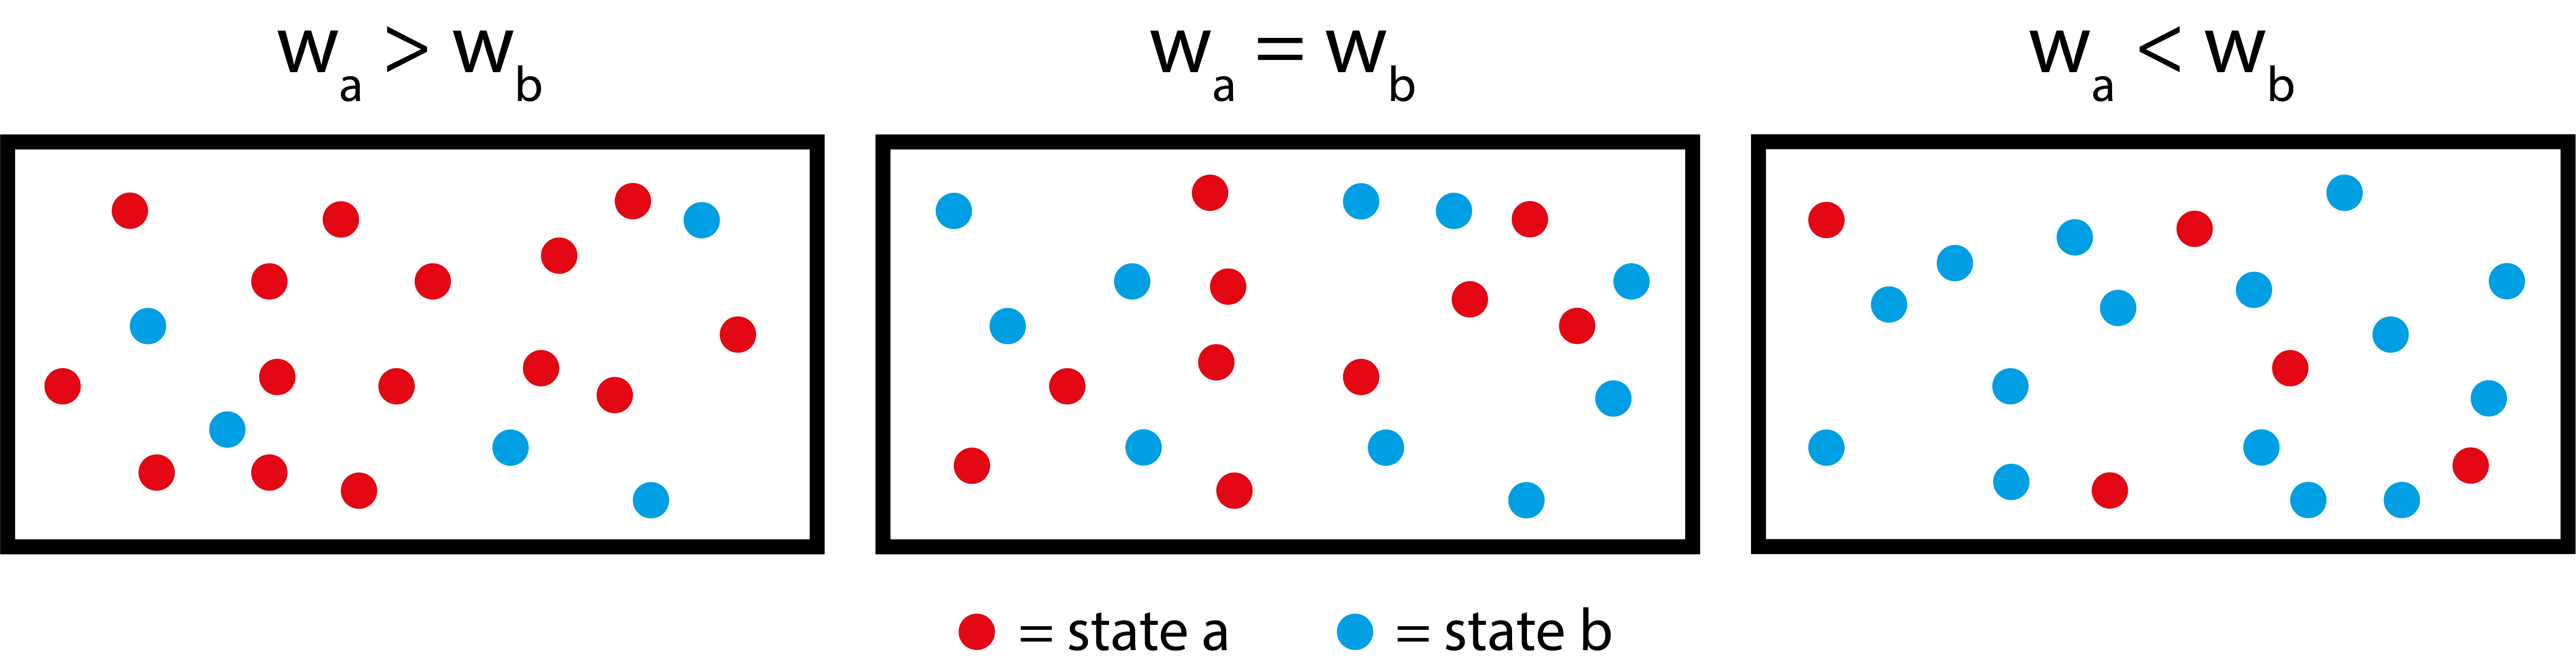
\includegraphics[scale=0.9]{thermodynamic_simple_example2}
\centering
\mycaption{Schematic of thermodynamic equilibrium for a substance exchanging between two states}{
As shown, the position of equilibrium depends on the standard chemical potentials of each state ($\mu_a^{\circ}$ and $\mu_b^{\circ}$).}
\label{fig:thermodynamic_simple_example2}
\end{figure}

We can apply a similar description to a species that is exchanging between two physical compartments. In this case \textbf{a} and \textbf{b} can represent material in two spatial compartments, with $\mu_a^{\circ}$ and $\mu_b^{\circ}$ representing the standard chemical potentials associated with each compartment. The chemical potential equations take on the same form as above, although we can make the following adjustment to the conservation of mass term to account for potential differences in the volume of the two compartments:
\begin{equation}
c_{tot} = c_a + \alpha c_b
\end{equation}

where $\alpha$ is a dimensionless factor comparing the volume of the two compartments. (In this case $c_{tot}$ can be interpreted as the concentration in compartment \textbf{a} when all molecules are in compartment \textbf{a}). As before, chemical equilibrium implies a linear relationship between concentrations in the two compartments, and the concentration ratio between compartments is specified by $\mu_b^{\circ} - \mu_a^{\circ}$ (\cref{fig:thermodynamic_simple_example}).\\

\begin{figure}
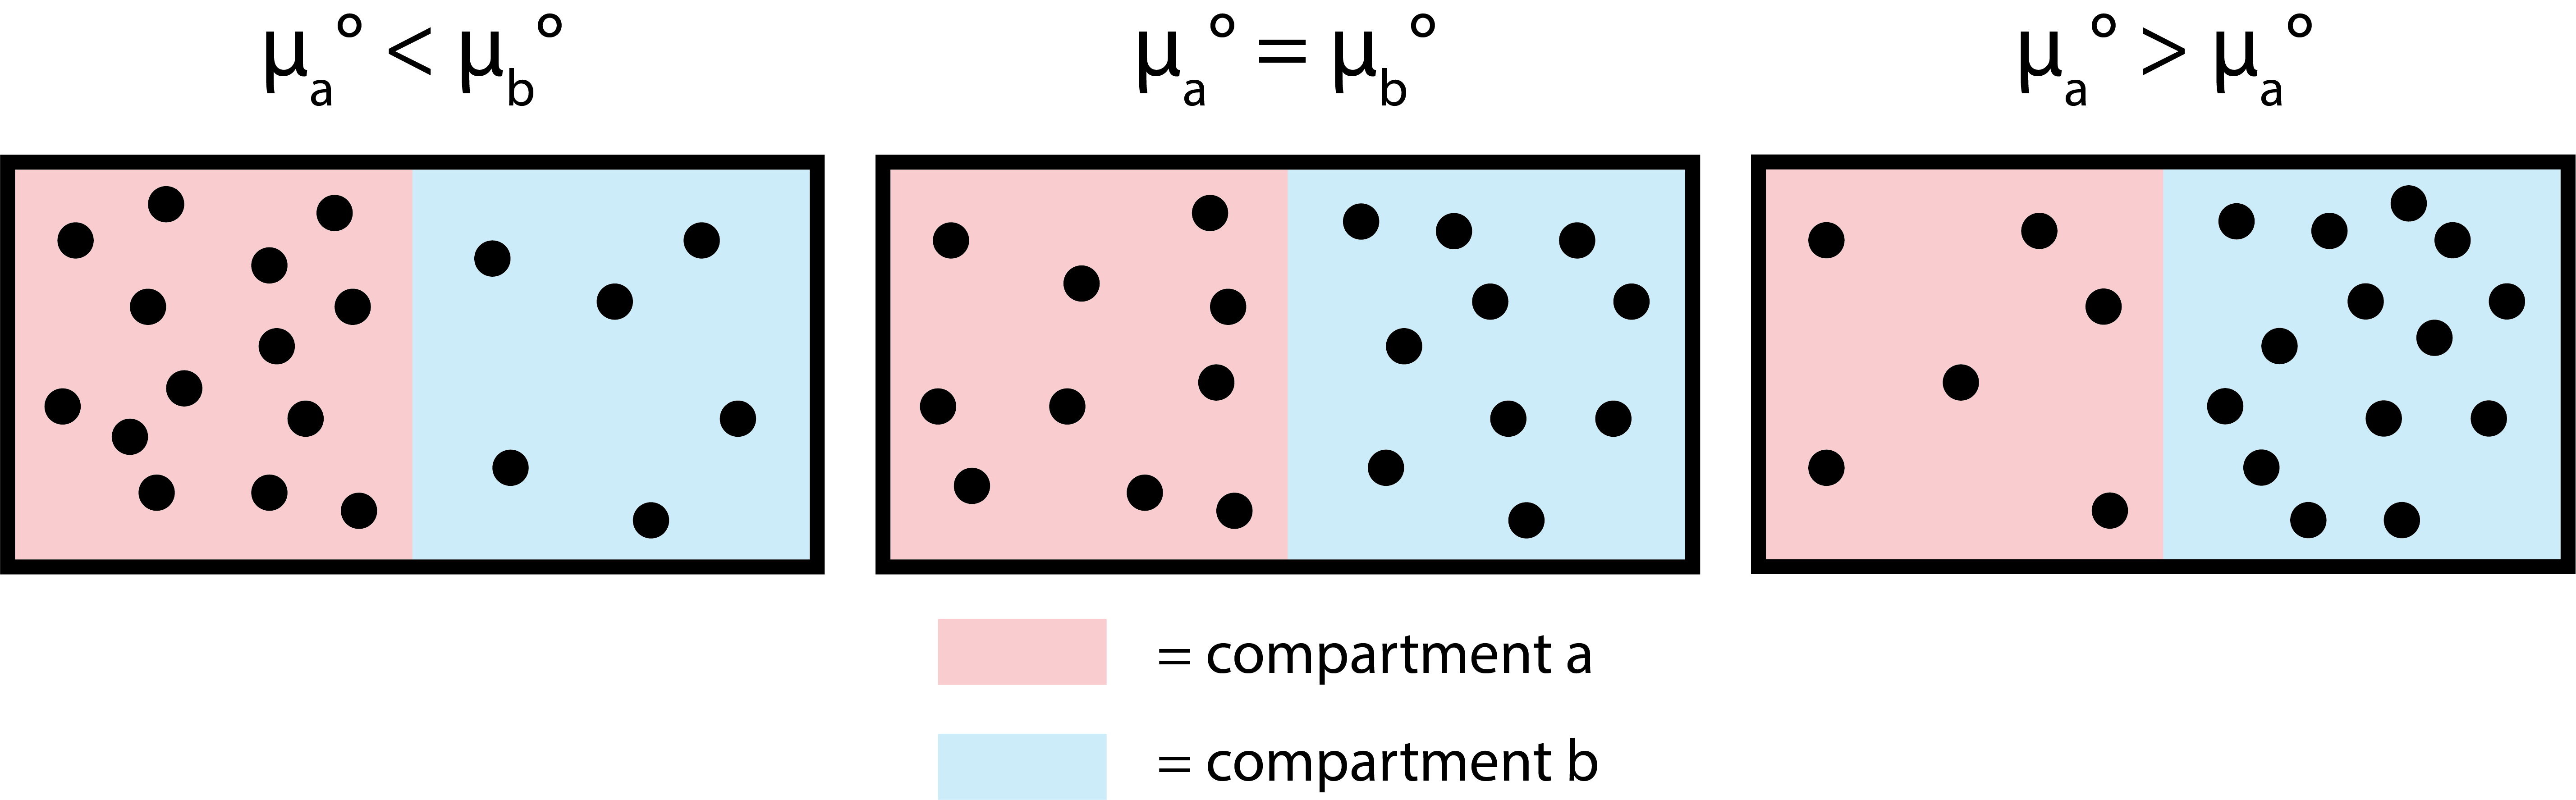
\includegraphics[scale=0.9]{thermodynamic_simple_example}
\centering
\mycaption{Schematic of thermodynamic equilibrium for a substance exchanging between two compartments}{
As shown, the position of equilibrium depends on the standard chemical potentials of the substance associated with each compartment ($\mu_a^{\circ}$ and $\mu_b^{\circ}$). In this example, the volume ratio between the compartments ($\alpha$) is equal to 1.}
\label{fig:thermodynamic_simple_example}
\end{figure}



\clearpage
\section{A thermodynamic model of dimerisation and membrane association}
\label{section:thermodynamic_full_model}

Now that I have introduced the modelling framework, we can begin to use this approach to understand the equilibrium behaviour of PAR-2 in a cellular environment. Specifically, I aim to model dimerisation of PAR-2, and its interaction with the plasma membrane, to understand how these behaviours might interact with each other. I will begin by building individual thermodynamic descriptions of membrane association and dimerisation, before describing a full model which combines both features.\\

\subsection{Thermodynamic description of membrane association}
\label{section:thermodynamic_membrane_binding}

PAR-2 binds to the inner surface of the plasma membrane via electrostatic charge, and undergoes a continuous exchange between membrane bound (\textbf{m}) and cytoplasmic (\textbf{c}) states:

\begin{center}
\ce{c <=> m}
\end{center}

At equilibrium, the forward and reverse reactions occur at equal rates, and concentrations have no tendency to change over time. For now, we can consider the \textit{par-3 (it71)} condition discussed in chapter 3, in which PAR-2 is not being phosphorylated by PKC-3 and lies uniformly on the membrane without diffusive fluxes, to be close to equilibrium. (In chapter 7 I will return to this point, and discuss conditions in which this may not be the case). \\

In the previous section I described an approach to model the equilibrium behaviour of a particle exchanging between two spatial compartments. We can use a similar description for a protein exchanging between membrane-bound and cytoplasmic states, by considering membrane and cytoplasm as two volume compartments. In this case the membrane compartment can be described as a thin volume between the plasma membrane and the cytoplasm (\cref{fig:thermodynamic_membrane_binding_schematic}). In this very simple description, if we assume that motion of membrane-bound molecules is confined to two dimensions along the inner surface of the plasma membrane, the effective thickness of the membrane compartment will be equal to the diameter of the protein ($D$). Therefore, the volume ratio between the two compartments can be given as $D\psi$, where $\psi$ is the surface area to volume ratio, and the total amount of protein can be described as:
\begin{equation}
c_{tot} = c_c + D\psi c_m
\end{equation}

where $c_m$ and $c_c$ are molar concentrations in the cytoplasmic and membrane compartments, and $c_{tot}$ is the total amount of protein (i.e. the cytoplasmic concentration when all molecules are cytoplasmic).\\

\begin{SCfigure}
\includegraphics[scale=1]{thermodynamic_membrane_binding_schematic}
\mycaption{Schematic of equilibrium model for membrane association}{
The system can be described as two volume compartments representing cytoplasmic and membrane-bound states. We assume that diffusion in the membrane compartment is confined to the two-dimensional plane of the plasma membrane, so the membrane compartment can be described as a volume with thickness $D$, where $D$ is equal to the diameter of the molecule.
}
\label{fig:thermodynamic_membrane_binding_schematic}
\end{SCfigure}

We can see from the analysis in the previous section that equilibrium concentrations depend only on the difference between $\mu^{\circ}$ terms. Therefore, for the purpose of determining equilibria, we can define chemical potentials as:
\begin{align}
\mu_c &= RT \ln \frac{c_c}{c^{\circ}}\\
\mu_m &= RT \ln \frac{c_m}{c^{\circ}} - w_m
\end{align} 

where $w_m$ represents the energetic difference between the cytoplasmic and membrane states (i.e. $\mu_c^{\circ} - \mu_m^{\circ}$). Therefore, similar to the description in section \ref{sec:modelling_chemical_equilibria}, membrane to cytoplasmic ratios at equilibrium are expected to be constant, according to the value of $w_m$:
\begin{equation}
\frac{c_m}{c_c} = e^{w_m/RT}
\end{equation}


\subsection{Thermodynamic description of dimerisation}

We can use similar analysis to consider a dimerisation reaction:

\begin{center}
\ce{2x_1 <=> x_2}
\end{center}

where x$_1$ represents a monomer and x$_2$ represents a dimer. Chemical potentials can be described as:
\begin{align}
\mu_{x_1} &= RT\ln \frac{c_{x_1}}{c^{\circ}} \\
\mu_{x_2} &= RT\ln  \frac{c_{x_2}}{c^{\circ}} - w_d
\end{align} 

where $w_d$ represents the dimerisation energy (i.e. the energetic difference between the monomeric and dimeric states ($\mu_{x1}^{\circ} - \mu_{x2}^{\circ}$)). Thermodynamic equilibrium is reached when $2\mu_{x_1} = \mu_{x_2}$ (the factor of 2 accounting for the differing stoichiometry between the two species), leading to the following relationship:
\begin{equation}
\frac{c_{x_2}\:c^{\circ}}{(c_{x_1})^2} = e^{w_d/RT}
\end{equation}

Therefore, concentrations of dimeric protein will vary with the square of monomer concentrations (\cref{fig:thermodynamic_simple_dimer}A). With the constraint that $c_{tot} = c_{x1} + c_{x2}$, we can derive relationships for the concentrations of monomer and dimer as a function of total protein:
\begin{align}
c_{x_1} &= \frac{1}{2}e^{-w_d/RT}\left(\sqrt{4e^{w_d/RT} \frac{c_{tot}}{c^{\circ}} + 1} - 1\right)c^{\circ}\\
c_{x_2} &= c_{tot} - \frac{1}{2}e^{-w_d/RT}\left(\sqrt{4e^{w_d/RT} \frac{c_{tot}}{c^{\circ}} + 1} - 1\right)c^{\circ}
\end{align}

Plotting these functions, we can see that the total fraction of protein in the dimeric state is expected to increase as a function of protein amounts (\cref{fig:thermodynamic_simple_dimer}B). Note that in this description, $c_{x_2}$ is related not to the number of dimer molecules but the number of protein monomers in the dimeric state.\\

\begin{figure}
\includegraphics[scale=1]{thermodynamic_simple_dimer}
\centering
\mycaption{Dimerisation reactions lead to nonlinear equilibrium behaviour}{
\textbf{(A)} At equilibrium, dimer concentrations vary with the square of monomer concentrations.
\textbf{(B)} The total fraction of protein in the dimeric state increases as the concentration of total material increases. Parameters used: $c^{\circ} = 1$ M, $w_d / RT = 10$. Concentrations in molar units.}
\label{fig:thermodynamic_simple_dimer}
\end{figure}


\subsection{Combining membrane association and dimerisation}

So far, I have explored how dimerisation and membrane binding reactions can be described in simple thermodynamic terms. In this section I combine these descriptions to explore the potential interplay between dimerisation and membrane binding.\\

In a system in which a protein is both dimerising and exchanging between membrane and cytoplasmic pools, there are four potential species to consider: membrane monomers (\textbf{m$_1$}), membrane dimers (\textbf{m$_2$}), cytoplasmic monomers (\textbf{c$_1$}) and cytoplasmic dimers (\textbf{c$_2$}) (\cref{fig:thermodynamic_model_species}A). We can describe chemical potentials for these four species as:
\begin{align}
\mu_{c_1} &= RT\ln(c_{c_1} / c^{\circ})\\
\mu_{c_2} &= RT\ln(c_{c_2} / c^{\circ}) - w_d\\
\mu_{m_1} &= RT\ln(c_{m_1} / c^{\circ}) - w_m\\
\mu_{m_2} &= RT\ln(c_{m_2} / c^{\circ}) - 2w_m - w_d
\end{align}

where $w_m$ is the membrane binding energy and $w_d$ is the dimerisation energy. Here, we assume that a molecule in a dimer has twice the membrane binding energy of monomer (as dimers have membrane binding interfaces from each of two monomers), and that the dimerisation energy is equal in the membrane and cytoplasm. Chemical equilibrium is reached when:
\begin{equation}
2\mu_{c_1} = \mu_{c_2} = 2\mu_{m_1} = \mu_{m_2}
\label{eq:four_species_equilibrium}
\end{equation}

Since the total amount of material is conserved, we have the initial constraint that:
\begin{align}
c_{tot} &= c_c + D \psi c_m
\label{eq:four_species_mass_conservation}
\end{align}

where $c_c = c_{c_1} + c_{c_2}$ and $c_m = c_{m_1} + c_{m_2}$, $D$ is the protein diameter, and $\psi$ is the surface area to volume ratio. For a given amount of total protein, equations \ref{eq:four_species_equilibrium} and \ref{eq:four_species_mass_conservation} can be solved to calculate equilibrium concentrations of each of the four species.\\

I first investigated how the equilibrium state of a system with a fixed total amount of protein ($c_{tot}$), varies depending on the two energy parameters: $w_m$ and $w_d$ (\cref{fig:thermodynamic_model_species}B). This analysis reveals that there are energy regimes in which each of the four states are favoured. With low $w_d$ and low $w_m$ protein will largely by cytoplasmic and monomeric; with low $w_d$ and high $w_m$ protein will be largely membrane-bound and monomeric; with high $w_d$ and low $w_m$ protein will be largely cytoplasmic and dimeric; and with high $w_d$ and high $w_m$ protein will be largely membrane-bound and dimeric. At intermediate energies a mix of states can be observed.\\

\begin{figure}
\includegraphics[scale=0.9]{thermodynamic_model_species}
\centering
\mycaption{The equilibrium state of a four-species dimerisation model varies depending on the interaction energies}{
\textbf{(A)} Schematic of the four species in the system.
\textbf{(B)} The equilibrium state as a function of the membrane association energy ($w_m$) and dimerisation energy ($w_d$). Shows the total amount of protein in each of the four states as a fraction of total protein. $c_{tot} / c^{\circ} = 10^{-5}$, $D\psi$ = 0.001}
\label{fig:thermodynamic_model_species}
\end{figure}

We can also see that the total amount of protein bound to the membrane ($m_1$ + $m_2$) varies according to both $w_m$ and $w_d$. By stabilising the high affinity dimeric state, increases to $w_d$ can increase overall membrane localisation for a constant $w_m$\\


\subsection{Intermediate dimerisation can drive nonlinear membrane association}

I next investigated how the system responds to varying total protein amounts. As previously described, the equilibrium state of dimerisation reactions varies as a function of total concentration, with more concentrated systems favouring increased dimerisation (\cref{fig:thermodynamic_simple_dimer}B). We would therefore expect that, in a model involving both dimerisation and membrane association, the equilibrium state should vary depending on total protein amounts.\\

In the absence of dimerisation, membrane and cytoplasmic concentrations have defined ratio (section \ref{section:thermodynamic_membrane_binding}), and therefore will vary linearly as protein amounts are changed. In a system in which protein can dimerise, this is no longer the case. Figure \ref{fig:thermodynamic_model_feedback} shows that, in certain parameter regimes, a nonlinear relationship can be observed between cytoplasmic and membrane concentrations, with an effective exponent varying between 1 (linear relationship) and 2 (quadratic relationship).\\

\begin{figure}
\includegraphics[scale=1]{thermodynamic_model_feedback}
\centering
\mycaption{Intermediate dimerisation can drive nonlinear membrane association}{
\textbf{(A)} The relationship between cytoplasmic and membrane concentrations at equilibrium, found by modelling systems with varying amounts of total protein (ranging from $c_{tot} = 10^{-7}$ to $c_{tot} = 10^{-5}$). Curves are colour coded according to the value of $w_d$, corresponding to the coloured points in (B).
\textbf{(B)} The effective exponent of the membrane versus cytoplasm relationship across parameter space. Exponents were calculated by fitting curves such as those shown in (A) to the equation $c_m/c^{\circ} = \alpha \: (c_c/c^{\circ})^{\beta}$, with $\beta$ taken as the effective exponent. $D\phi$ = 0.001.
}
\label{fig:thermodynamic_model_feedback}
\end{figure}

Peak nonlinearity occurs in regions with high membrane energy and intermediate dimerisation energy. This corresponds to regions of parameter space in which membrane protein is largely dimeric but cytoplasmic protein largely monomeric, across the relevant range of total protein amounts (\cref{fig:thermodynamic_model_dimer_fractions}). When $w_d$ is low, protein is unable to dimerise, even at enriched membrane concentrations, and so the system follows simple linear behaviour like the monomer system described in section \ref{section:thermodynamic_membrane_binding}. If, on the other hand, $w_d$ is too high, protein is fully dimeric in both the membrane and cytoplasm, and so the system will behave similarly to the monomeric system (albeit with a higher membrane affinity). If, on the other hand, $w_d$ is intermediate, then an asymmetry can be observed whereby protein is dimeric on the membrane but not in the cytoplasm, provided that $w_m$ is sufficiently large to set up a substantial concentration difference between the two compartments.\\

\begin{figure}
\includegraphics[scale=0.9]{thermodynamic_model_dimer_fractions}
\centering
\mycaption{The dimeric state of cytoplasmic and membrane protein as a function of $w_m$, $w_d$ and $c_{tot}$}{
Figure shows the fraction of total membrane protein (A) and total cytoplasmic protein (B) that is dimeric in models with varying $w_m$, $w_d$ and $c_{tot}$. Comparing this with \cref{fig:thermodynamic_model_feedback}, we can see that regions of peak nonlinearity occur when membrane protein is dimeric but cytoplasmic protein monomeric.
}
\label{fig:thermodynamic_model_dimer_fractions}
\end{figure}

To understand why this leads to a nonlinear membrane binding relationship, consider an extreme case in which all cytoplasmic protein is monomeric and all membrane protein is dimeric (with the other two states being transient intermediates). In other words, we have the following equilibrium:

\begin{center}
\ce{2c_1 <=> m_2}
\end{center}

Solving for $2\mu_{c1} = \mu_{m2}$ at equilibrium, we obtain the following relationship:
\begin{equation}
\frac{c_{m2}}{c^{\circ}} = e^{2w_m + w_d} \left(\frac{c_{c1}}{c^{\circ}}\right)^2
\end{equation}

implying a quadratic relationship between cytoplasmic and membrane concentrations.\\

Overall, this analysis shows that dimerisation can have a strong influence on the membrane binding behaviour of a protein. With the assumption that the membrane binding energy of a dimer is twice that of a monomer, dimerisation is expected to strongly enhance membrane affinity and overall membrane localisation. I have also shown that nonlinear membrane association behaviour can arise if dimerisation and membrane binding energies are sufficient to so that dimerisation is supported on the membrane but not in the cytoplasm.\\

\clearpage
\section{Quantitative assessment of PAR-2 membrane association behaviour}

Several features of this model are particularly relevant for PAR-2. Firstly, the model suggests that a reduction in dimerisation energy ($w_d$), as would be expected for a RING-disrupting mutant, can substantially decrease membrane association, independently of the membrane association energy ($w_m$). Secondly, the model suggests that, in some parameter regimes, a nonlinear relationship can occur between cytoplasmic and membrane concentrations. This latter point has the condition that dimerisation be supported in the membrane but not the cytoplasm, both of which appear to be the case for PAR-2 in vivo.\\

To assess how well the membrane-binding behaviour of wild type and RING-mutant PAR-2 can be captured by this model, I performed a quantitative comparison of the model to in vivo measurements of cytoplasmic and membrane PAR-2 concentrations. I first asked whether the different membrane-binding behaviour of wild type and RING mutant PAR-2 can be explained purely by a difference in dimerisation energies. \\

In chapter 3, I showed that wild type PAR-2 has displays nonlinear membrane association, which is disrupted in a C56S RING domain mutant. In light of results described in the chapter 4, which suggest that C56S may disrupt membrane binding by more than just disrupting dimerisation, I decided to repeat the rundown experiment described in section \ref{section:par2_rundown} using the L109R mutant as a baseline instead of C56S. The results show a similar effect, whereby L109R mutant PAR-2 follows a shallower, more linear trajectory compared to wild type PAR-2 (\cref{fig:thermodynamic_wt_vs_l109r_model_fit}).\\

% Do the same fig here to show cyt vs mem relationship?


% Ultimately this parameter influences the degree to effective concentrations are enhanced upon membrane binding, which will influence the degree to which dimeric state can differ in the membrane and cytoplasmic compartments.

To assess whether the different behaviour of WT and L109R can be explained purely by a reduction in dimerisation energy, I fit the in vivo data to a model in which $w_m$ is unchanged between the two conditions but $w_d$ allowed to change. As discussed previously, the model has a parameter $D$ describing the diameter of the protein molecule. Whilst this has not been determined for PAR-2, we can expect that, with a mass of 69.95 kDa, protein diameter should be on the order of 1-10 nm \citep{Erickson2009}. To assess the full range of model behaviours I consider $D$ at both extremes.\\

I performed model fitting by orthogonal distance regression, and estimated parameter uncertainty by bootstrapping (\cref{fig:thermodynamic_wt_vs_l109r_model_fit}A, C). Optimised model parameters and 95\% confidence intervals are shown in table \ref{table:thermodynamic_model_parameters}.\\

\begin{table}[]
\begin{tabular}{|l|l|l|}
\hline
 & \textbf{Model 1 (D = 10 nm)} & \textbf{Model 2 (D = 1 nm)} \\ \hline
$w_m/RT$ & 5.94 {[}5.63, 6.10{]} & 8.24 {[}7.96, 8.41{]} \\ \hline
$w_d/RT$ (WT) & 12.99 {[}12.39, 13.88{]} &  {[}10.09, 11.51{]}\\ \hline
$w_d/RT$ (L109R) & 11.16 {[}10.16, 12.46{]} & 8.84 {[}7.83, 10.11{]} \\ \hline
$w_d/RT$ difference & 1.83 {[}1.36, 2.27{]} & 1.83 {[}1.36, 2.28{]} \\ \hline
kD fold difference & 6.21 {[}3.89, 9.69{]} & 6.22 {[}3.90, 9.81{]} \\ \hline
\end{tabular}

\mycaption{Optimised model parameters}{
Given for models in which $D$ (protein diameter) = 10 nm or 1 nm. Both models show that the data is best explained by an approximately 6-fold difference in dimerisation kD between wild type and L109R PAR-2. 95\% confidence intervals shown in square brackets.
}

\label{table:thermodynamic_model_parameters}
\end{table}

Figures \ref{fig:thermodynamic_wt_vs_l109r_model_fit}B and D show that the optimised models closely capture the data, suggesting that a reduction in dimerisation energy by approximately 1.8 $RT$ is sufficient to account for the different membrane association relationships of wild type PAR-2 and PAR-2 L109R. This corresponds to a roughly 6-fold difference in the dissociation constant (kD). (Note that the dissociation constant (kD) for dimerisation is exponentially related to the dimerisation energy, so a decrease in $w_d / RT$ by $x$ corresponds to a $e^x$ fold increase in kD.) Furthermore, we can see that the optimised models predict that cytoplasmic protein is entirely monomeric across the range of relevant concentrations, whereas wild type membrane-bound protein is mostly dimeric, which matches experimental observations. Dimerisation of PAR-2 L109R is reduced at the membrane compared to wild type PAR-2.

% Maybe have a box for model fitting procedure?

\begin{figure}
\includegraphics[scale=0.85]{thermodynamic_wt_vs_l109r_model_fit}
\centering
\mycaption{Membrane-association behaviour of wild-type and L109R PAR-2 can be explained by a reduction in dimerisation energy}{
\textbf{(A, C)} Parameter estimates for models with $D$ (protein diameter) = 10 nm (A) or 1 nm (C). Models were fit to the in vivo data in (B) and (C) by orthogonal distance regression. Parameter uncertainty was assessed by bootstrapping. Each point represents parameters obtained from fitting a model to single bootstrap sample (an orange and a blue point with a shared $w_m$ for each sample). Black dots show parameters for a model trained on the full dataset.
\textbf{(B, D)} In vivo data (points) compared to model fits (lines, shaded regions indicate 95\% confidence intervals). $c^{\circ}$ is defined as the mean cytoplasmic concentration of wild type PAR-2 at full dosage x $10^8$. Assuming a cytoplasmic concentration of roughly 10 nM \citep{Gross2018}, this corresponds to approximately 1 M. Also shown are the dimeric states of membrane and cytoplasmic protein in the models across the range of concentrations, with 95\% confidence intervals.
}
\label{fig:thermodynamic_wt_vs_l109r_model_fit}
\end{figure}



\section{Discussion}

Overall, this analysis shows that a number of previously unexplained behaviours of PAR-2 can be explained by the ability its ability to dimerise. The in vitro data in chapter 4 shows that the PAR-2 RING domain displays concentration dependent dimerisation. I propose that, in vivo, cytoplasmic PAR-2 concentrations are too low for the RING to dimerise, but enrichment on the membrane enhances effective concentrations, driving concentration-dependent RING dimerisation on the membrane. This reaction has two major consequences:\\

Firstly, as dimers can utilise membrane binding interfaces from two PAR-2 molecules, dimerisation is expected to overall membrane affinities. This provides an explanation for the reduction in membrane localisation seen for all RING domain mutants (chapter 4). \\

Secondly membrane-specific dimerisation can lead to a nonlinear membrane association relationship, which closely matches in vivo PAR-2 data. The model makes a number of simplifications in its description of interaction energies, such as the assumption that dimerisation energy is equal in the cytoplasm and on the membrane, and that dimers have a membrane association energy twice that of a monomer. Nevertheless, a general feature of the model, shown by equation x, is that, regardless of the values of the energy terms, as long as the system can achieve dimerisation on the membrane but not in the cytoplasm, a quadratic relationship between cytoplasmic and membrane concentrations is to be expected.\\

This nonlinearity can be considered a form of positive feedback in which the effective membrane affinity increases with increasing membrane concentrations. Oligomerisation is a common feature of many polarity proteins, and has been suggested to contribute to stable bistability in mathematical models of polarity \citep{Lang2022}. In the next chapter, I consider the specific impact that PAR-2 dimerisation may have on the patterning behaviour of the PAR network.\\

% The question remains as to why C56S appears more disruptive than L109R. One possibility is that dimerisation isn’t completely disrupted in L109R, although if this were the case, I’d expect L109R and L50R to be additive, which they are not. Another possibility is that C56S mutation, by causing the entire domain to unfold, has an additional negative impact on membrane binding whereby the unfolded domain interferes with the association between the polybasic domain and the membrane (effectively causing a decrease in $w_m$ in addition to $w_d$).\\

%%%%%%%%%%%%%%%%%%%%%%%%%%%%%%%%%%%%%%%%%%%%%%%%%%%%%%%%%%
\clearpage
\chapter{Modelling dimerisation-driven positive feedback in the PAR network}

\textbf{Detailed contributions:}\\

\clearpage
\section{Model description}

\subsection{Reducing thermodynamic model to a two-species model} 

To simplify further analysis, we can convert the four species thermodynamic model to a two species model, in which we only track overall membrane and cytoplasmic concentrations, $\phi_m$ and $\phi_c$, irrespective of dimeric state. If we assume that dimerisation reactions in the membrane and cytoplasm are fast relative to membrane binding, we can define instantaneous monomer and dimer concentrations as a function of overall concentration. For example, for cytoplasmic protein:
% check equations
\begin{align}
\phi_{c,1} &= \frac{1}{2}e^{-w_d}\left(\sqrt{4e^{w_d}\phi_c + 1} - 1\right)\\
\phi_{c,2} &= \phi_c - \frac{1}{2}e^{-w_d}\left(\sqrt{4e^{w_d}\phi_c + 1} - 1\right)
\end{align}

which is identical to the description in section x. As a result, and because we can describe the chemical potential of each of these species individually (equations xxx), we can combine expression <> and <> to define the overall chemical potential of cytoplasmic protein ($\mu_c$) as a function of overall cytoplasmic concentrations ($\phi_c$):
\begin{equation}
\mu_c = \ln(\phi_c) - \frac{1}{2}\ln\left(1 + 2e^{w_d}\phi_c + \sqrt{4e^{w_d}\phi_c + 1}\right)
\end{equation}
% check equation

And analogously for membrane bound protein: 
\begin{equation}
\mu_m = \ln(\phi_m) - \frac{1}{2}\ln\left(1 + 2e^{w_d}\phi_m + \sqrt{4e^{w_d}\phi_m + 1}\right) - w_m
\end{equation}
% check equation

These two equations can be solved analytically at equilibrium ($\mu_c$ = $\mu_m$) to find equilibrium membrane and cytoplasmic concentrations.


\subsection{Explicit description of membrane binding kinetics} 

Building kinetic models requires a description of membrane and unbinding rates, rather than just energetics. Exchange can be written as:

\begin{center}
\ce{$\phi_c$ <=>[$k_{on}$][$k_{off}$] $\phi_m$}
\end{center}

For a given composition, flux on ($s_{on}$) is equal to $k_{on}\phi_c$, and flux off ($s_{off}$) is equal to $k_{off}\phi_m$. Using transition state theory, these fluxes can be written as:
\begin{align}
s_{on} &= ke^{\mu_c}\\
s_{off} &= ke^{\mu_m}
\end{align}

where $k$ is a kinetic factor. Using our previous descriptions of cytoplasmic and membrane chemical potentials, the kinetic rate constants can be calculated as:
\begin{align}
k_{on} &= \frac{k}{\sqrt{2e^{w_d}\phi_c+ 1}}\\
k_{off} &= \frac{ke^{-w_m}}{\sqrt{2e^{w_d}\phi_m+ 1}}
\end{align}

implying a dependence on both energies and concentrations. This is shown for $k_{off}$ in fig x. Fig xA shows off rates plot a function of membrane energy and dimerisation energy, for a given membrane concentration. We can also see (fig xB), the dependence of off rates on concentrations.

\begin{figure}[!h]
\includegraphics[scale=1]{thermodynamic_model_koff}
\setlength{\abovecaptionskip}{20pt}
\centering
\mycaption{Title}{Caption}
\label{fig:thermodynamic_model_koff}
\end{figure}

\subsection{Incorporation into mutual antagonism model}


%%%%%%%%%%%%%%%%%%%%%%%%%%%%%%%%%%%%%%%%%%%%%%%%%%%%%%%%%%
\clearpage
\chapter{Experimental manipulation of PAR-2 dimerisation}

\textbf{Detailed contributions:}\\

\clearpage
\section{Introduction}

\section{Forced constitutive dimerisation of PAR-2 shifts localisation towards lower-affinity membranes}

% Strikingly, we see the unexpected appearance of visible structures within the cell. Based on comparison to RAB localisation patterns, these appear to be endosomes.

% We also see the appearance of PAR-2 on the anterior membrane, suggesting that the protein is less susceptable to antagonism by PKC-3

\begin{figure}[!h]
\includegraphics[scale=1]{gcn4}
\setlength{\abovecaptionskip}{20pt}
\centering
\mycaption{Title}{Caption}
\label{fig:gcn4}
\end{figure}

\begin{figure}[!h]
\includegraphics[scale=1]{gcn4_quantification}
\setlength{\abovecaptionskip}{20pt}
\centering
\mycaption{Title}{Caption}
\label{fig:gcn4_quantification}
\end{figure}

\begin{figure}[!h]
\includegraphics[scale=1]{gcn4_alone}
\setlength{\abovecaptionskip}{20pt}
\centering
\mycaption{Title}{Caption}
\label{fig:gcn4_alone}
\end{figure}

\clearpage
\section{Incorporating internal membranes into the thermodynamic model}

I consider two further species, representing monomers and dimers bound to internal membranes.  Concentrations are specified by $\phi_{i,1}$ and $\phi_{i,2}$, chemical potentials $\mu_{i,1}$ and $\mu_{i,2}$ with energy parameters $w_{i,1}$ and $w_{i,2}$, where:

\begin{align}
w_{i,1} &= w_i\\
w_{i,2} &= 2w_i + w_d
\end{align}

where $w_i$ is the internal membrane insertion energy. Thermodynamic equilibrium is reached when:
\begin{equation}
2\mu_{c,1} =  \mu_{c,2} = 2\mu_{p,1} =  \mu_{p,2} = 2\mu_{i,1} =  \mu_{i,2}
\end{equation}

The total amount of protein is conserved according the the following:
\begin{equation}
\overline{\phi} = \phi_c + \alpha\phi_p + \beta\phi_i
\end{equation}

where $\alpha$ is a non-dimensional conversion factor between cytoplasmic and plasma membrane volume fractions, $\beta$ is the equivalent factor for internal membranes. Setting $\overline{\phi}$ as a fixed value, $\phi_{c,1}$, $\phi_{c,2}$, $\phi_{m,1}$, $\phi_{m,2}$, $\phi_{i,1}$ and $\phi_{i,2}$ can be solved numerically. Using this model, we can investigate the relationship between dimerisation energy ($w_d$) and PAR-2 localisation in systems with varying levels of internal membrane charge (varying $w_i$). As shown in fig x, we can see that, in systems where $w_i$ is sufficiently high, constitutive dimerisation (high $w_d$) can result in considerable PAR-2 levels on internal membranes, which isn't observed at lower/intermediate dimerisation strengths. 

\begin{figure}[!h]
\includegraphics[scale=0.90]{six_species_thermodynamic}
\setlength{\abovecaptionskip}{20pt}
\centering
\mycaption{Title}{Caption}
\label{fig:six_species_thermodynamic}
\end{figure}

% Whilst increasing wd may increase binding to internal membranes (provided that wi is high enough), this should always be accompanied by an increase in levels at the plasma membrane. In other words, we cannot get a scenario akin to what we see in vivo,  whereby constitutive dimerisation actually reduces levels on the plasma membrane.


\section{Modelling kinetics outside of equilibrium}


\begin{figure}[!h]
\includegraphics[scale=0.95]{three_surface_kinetic}
\setlength{\abovecaptionskip}{20pt}
\centering
\mycaption{Title}{Caption}
\label{fig:three_surface_kinetic}
\end{figure}


\section{aPAR disruption partially restores expected equilibrium localisation pattern}

\begin{figure}[!h]
\includegraphics[scale=0.95]{gcn4_par3mut}
\setlength{\abovecaptionskip}{20pt}
\centering
\mycaption{Title}{Caption}
\label{fig:gcn4_par3mut}
\end{figure}

\section{Discussion}



%%%%%%%%%%%%%%%%%%%%%%%%%%%%%%%%%%%%%%%%%%%%%%%%%%%%%%%%%%
\clearpage
\chapter{Discussion}


%%%%%%%%%%%%%%%%%%%%%%%%%%%%%%%%%%%%%%%%%%%%%%%%%%%%%%%%%%
\clearpage
\chapter{Materials and methods}

\clearpage
\section{Worm maintenance}
\section{Generating transgenic lines by CRISPR}

\begin{figure}[!h]
\includegraphics[scale=1]{glh}
\setlength{\abovecaptionskip}{20pt}
\centering
\mycaption{Title}{Caption}
\label{fig:glh}
\end{figure}



\section{Microscopy}
\section{Full-length PAR-2 purification}
\section{Ubiquitination assays}
\section{PAR-2 RING domain fragment purification}
\section{SEC-MALS}
\section{Image analysis}
\section{Modelling methods}

%%%%%%%%%%%%%%%%%%%%%%%%%%%%%%%%%%%%%%%%%%%%%%%%%%%%%%%%%%
\clearpage
\chapter*{Appendix: Analysis of PAR-2 diffusion kinetics by single particle tracking}
\addcontentsline{toc}{chapter}{Appendix: Analysis of PAR-2 diffusion kinetics by single particle tracking}




%%%%%%%%%%%%%%%%%%%%%%%%%%%%%%%%%%%%%%%%%%%%%%%%%%%%%%%%%%
\clearpage
\chapter*{Abbreviations}
\addcontentsline{toc}{chapter}{Abbreviations}




%%%%%%%%%%%%%%%%%%%%%%%%%%%%%%%%%%%%%%%%%%%%%%%%%%%%%%%%%%

\clearpage
\addcontentsline{toc}{chapter}{Bibliography}

\printbibliography

\end{document}
